\documentclass[a4paper]{book}
\usepackage{a4wide}
\usepackage{makeidx}
\usepackage{fancyhdr}
\usepackage{graphicx}
\usepackage{multicol}
\usepackage{float}
\usepackage{textcomp}
\usepackage{alltt}
\usepackage{times}
\usepackage{ifpdf}
\ifpdf
\usepackage[pdftex,
            pagebackref=true,
            colorlinks=true,
            linkcolor=blue,
            unicode
           ]{hyperref}
\else
\usepackage[ps2pdf,
            pagebackref=true,
            colorlinks=true,
            linkcolor=blue,
            unicode
           ]{hyperref}
\usepackage{pspicture}
\fi
\usepackage[utf8]{inputenc}
\usepackage{doxygen}
\makeindex
\setcounter{tocdepth}{3}
\renewcommand{\footrulewidth}{0.4pt}
\begin{document}
\begin{titlepage}
\vspace*{7cm}
\begin{center}
{\Large kgl \\[1ex]\large 0.1 }\\
\vspace*{1cm}
{\large Generated by Doxygen 1.5.8}\\
\vspace*{0.5cm}
{\small Thu Sep 3 23:25:17 2009}\\
\end{center}
\end{titlepage}
\clearemptydoublepage
\pagenumbering{roman}
\tableofcontents
\clearemptydoublepage
\pagenumbering{arabic}
\chapter{Class Index}
\section{Class Hierarchy}
This inheritance list is sorted roughly, but not completely, alphabetically:\begin{CompactList}
\item \contentsline{section}{KGLBaseItem}{\pageref{class_k_g_l_base_item}}{}
\begin{CompactList}
\item \contentsline{section}{KGLItem}{\pageref{class_k_g_l_item}}{}
\begin{CompactList}
\item \contentsline{section}{KGLAnimItem}{\pageref{class_k_g_l_anim_item}}{}
\item \contentsline{section}{KGLBoxItem}{\pageref{class_k_g_l_box_item}}{}
\begin{CompactList}
\item \contentsline{section}{KGLPixmapItem}{\pageref{class_k_g_l_pixmap_item}}{}
\end{CompactList}
\item \contentsline{section}{KGLCircleItem}{\pageref{class_k_g_l_circle_item}}{}
\item \contentsline{section}{KGLContainerItem}{\pageref{class_k_g_l_container_item}}{}
\begin{CompactList}
\item \contentsline{section}{KGLIntroItem}{\pageref{class_k_g_l_intro_item}}{}
\end{CompactList}
\item \contentsline{section}{KGLGridItem}{\pageref{class_k_g_l_grid_item}}{}
\item \contentsline{section}{KGLParticlesItem}{\pageref{class_k_g_l_particles_item}}{}
\item \contentsline{section}{KGLPhysicsItem}{\pageref{class_k_g_l_physics_item}}{}
\item \contentsline{section}{KGLPolygonItem}{\pageref{class_k_g_l_polygon_item}}{}
\item \contentsline{section}{KGLShadowItem}{\pageref{class_k_g_l_shadow_item}}{}
\item \contentsline{section}{KGLShadowItem}{\pageref{class_k_g_l_shadow_item}}{}
\item \contentsline{section}{KGLTextItem}{\pageref{class_k_g_l_text_item}}{}
\end{CompactList}
\end{CompactList}
\item \contentsline{section}{KGLContactListener}{\pageref{class_k_g_l_contact_listener}}{}
\item \contentsline{section}{KGLEngine}{\pageref{class_k_g_l_engine}}{}
\begin{CompactList}
\item \contentsline{section}{KGLPhysicsEngine}{\pageref{class_k_g_l_physics_engine}}{}
\end{CompactList}
\item \contentsline{section}{KGLFx}{\pageref{class_k_g_l_fx}}{}
\begin{CompactList}
\item \contentsline{section}{KGLBlurFx}{\pageref{class_k_g_l_blur_fx}}{}
\item \contentsline{section}{KGLLightFx}{\pageref{class_k_g_l_light_fx}}{}
\item \contentsline{section}{KGLPixelateFx}{\pageref{class_k_g_l_pixelate_fx}}{}
\end{CompactList}
\item \contentsline{section}{KGLItemList}{\pageref{class_k_g_l_item_list}}{}
\item \contentsline{section}{KGLParticle}{\pageref{class_k_g_l_particle}}{}
\item \contentsline{section}{KGLPoint}{\pageref{class_k_g_l_point}}{}
\item \contentsline{section}{KGLPointList}{\pageref{class_k_g_l_point_list}}{}
\item \contentsline{section}{KGLProgram}{\pageref{class_k_g_l_program}}{}
\item \contentsline{section}{KGLScreenConfig}{\pageref{class_k_g_l_screen_config}}{}
\item \contentsline{section}{KGLShader}{\pageref{class_k_g_l_shader}}{}
\begin{CompactList}
\item \contentsline{section}{KGLFragmentShader}{\pageref{class_k_g_l_fragment_shader}}{}
\item \contentsline{section}{KGLVertexShader}{\pageref{class_k_g_l_vertex_shader}}{}
\end{CompactList}
\item \contentsline{section}{KGLTexture}{\pageref{class_k_g_l_texture}}{}
\item \contentsline{section}{KGLView}{\pageref{class_k_g_l_view}}{}
\end{CompactList}

\chapter{Class Index}
\section{Class List}
Here are the classes, structs, unions and interfaces with brief descriptions:\begin{CompactList}
\item\contentsline{section}{\hyperlink{class_abs_val}{AbsVal} }{\pageref{class_abs_val}}{}
\item\contentsline{section}{\hyperlink{class_k_c_l_code}{KCLCode} }{\pageref{class_k_c_l_code}}{}
\item\contentsline{section}{\hyperlink{class_k_c_l_device_model}{KCLDeviceModel} }{\pageref{class_k_c_l_device_model}}{}
\item\contentsline{section}{\hyperlink{class_k_c_l_engine}{KCLEngine} }{\pageref{class_k_c_l_engine}}{}
\item\contentsline{section}{\hyperlink{class_k_c_l_info_widget}{KCLInfoWidget} }{\pageref{class_k_c_l_info_widget}}{}
\item\contentsline{section}{\hyperlink{class_k_c_l_input}{KCLInput} (Provide an object that represent an input. This is the class mother of all device you want to use. It return you all information about the device, for example the name. And it return the status of the device, it means the type, code, and value )}{\pageref{class_k_c_l_input}}{}
\item\contentsline{section}{\hyperlink{class_k_c_l_input_event}{KCLInputEvent} (Provides a input events )}{\pageref{class_k_c_l_input_event}}{}
\item\contentsline{section}{\hyperlink{class_k_c_l_joystick}{KCLJoystick} }{\pageref{class_k_c_l_joystick}}{}
\item\contentsline{section}{\hyperlink{class_k_c_l_key_board}{KCLKeyBoard} }{\pageref{class_k_c_l_key_board}}{}
\item\contentsline{section}{\hyperlink{class_k_c_l_mouse}{KCLMouse} }{\pageref{class_k_c_l_mouse}}{}
\item\contentsline{section}{\hyperlink{class_k_c_l_thread}{KCLThread} (Provides a QThread witch listen the input status )}{\pageref{class_k_c_l_thread}}{}
\item\contentsline{section}{\hyperlink{class_virtual_button}{VirtualButton} }{\pageref{class_virtual_button}}{}
\end{CompactList}

\chapter{File Index}
\section{File List}
Here is a list of all files with brief descriptions:\begin{CompactList}
\item\contentsline{section}{/home/sacha/programmation/gluon/kal/\hyperlink{kalbuffer_8cpp}{kalbuffer.cpp} }{\pageref{kalbuffer_8cpp}}{}
\item\contentsline{section}{/home/sacha/programmation/gluon/kal/\hyperlink{kalbuffer_8h}{kalbuffer.h} }{\pageref{kalbuffer_8h}}{}
\item\contentsline{section}{/home/sacha/programmation/gluon/kal/\hyperlink{kalcapture_8cpp}{kalcapture.cpp} }{\pageref{kalcapture_8cpp}}{}
\item\contentsline{section}{/home/sacha/programmation/gluon/kal/\hyperlink{kalcapture_8h}{kalcapture.h} }{\pageref{kalcapture_8h}}{}
\item\contentsline{section}{/home/sacha/programmation/gluon/kal/\hyperlink{kalengine_8cpp}{kalengine.cpp} }{\pageref{kalengine_8cpp}}{}
\item\contentsline{section}{/home/sacha/programmation/gluon/kal/\hyperlink{kalengine_8h}{kalengine.h} }{\pageref{kalengine_8h}}{}
\item\contentsline{section}{/home/sacha/programmation/gluon/kal/\hyperlink{kalengine__export_8h}{kalengine\_\-export.h} }{\pageref{kalengine__export_8h}}{}
\item\contentsline{section}{/home/sacha/programmation/gluon/kal/\hyperlink{kalinfowidget_8cpp}{kalinfowidget.cpp} }{\pageref{kalinfowidget_8cpp}}{}
\item\contentsline{section}{/home/sacha/programmation/gluon/kal/\hyperlink{kalinfowidget_8h}{kalinfowidget.h} }{\pageref{kalinfowidget_8h}}{}
\item\contentsline{section}{/home/sacha/programmation/gluon/kal/\hyperlink{kaloggstreamer_8cpp}{kaloggstreamer.cpp} }{\pageref{kaloggstreamer_8cpp}}{}
\item\contentsline{section}{/home/sacha/programmation/gluon/kal/\hyperlink{kaloggstreamer_8h}{kaloggstreamer.h} }{\pageref{kaloggstreamer_8h}}{}
\item\contentsline{section}{/home/sacha/programmation/gluon/kal/\hyperlink{kalphonon_8cpp}{kalphonon.cpp} }{\pageref{kalphonon_8cpp}}{}
\item\contentsline{section}{/home/sacha/programmation/gluon/kal/\hyperlink{kalphonon_8h}{kalphonon.h} }{\pageref{kalphonon_8h}}{}
\item\contentsline{section}{/home/sacha/programmation/gluon/kal/\hyperlink{kalsoundloader_8cpp}{kalsoundloader.cpp} }{\pageref{kalsoundloader_8cpp}}{}
\item\contentsline{section}{/home/sacha/programmation/gluon/kal/\hyperlink{kalsoundloader_8h}{kalsoundloader.h} }{\pageref{kalsoundloader_8h}}{}
\item\contentsline{section}{/home/sacha/programmation/gluon/kal/\hyperlink{kalsource_8cpp}{kalsource.cpp} }{\pageref{kalsource_8cpp}}{}
\item\contentsline{section}{/home/sacha/programmation/gluon/kal/\hyperlink{kalsource_8h}{kalsource.h} }{\pageref{kalsource_8h}}{}
\end{CompactList}

\chapter{Class Documentation}
\hypertarget{class_k_g_l_anim_item}{
\section{KGLAnimItem Class Reference}
\label{class_k_g_l_anim_item}\index{KGLAnimItem@{KGLAnimItem}}
}
{\tt \#include $<$kglanimitem.h$>$}

Inheritance diagram for KGLAnimItem::\begin{figure}[H]
\begin{center}
\leavevmode
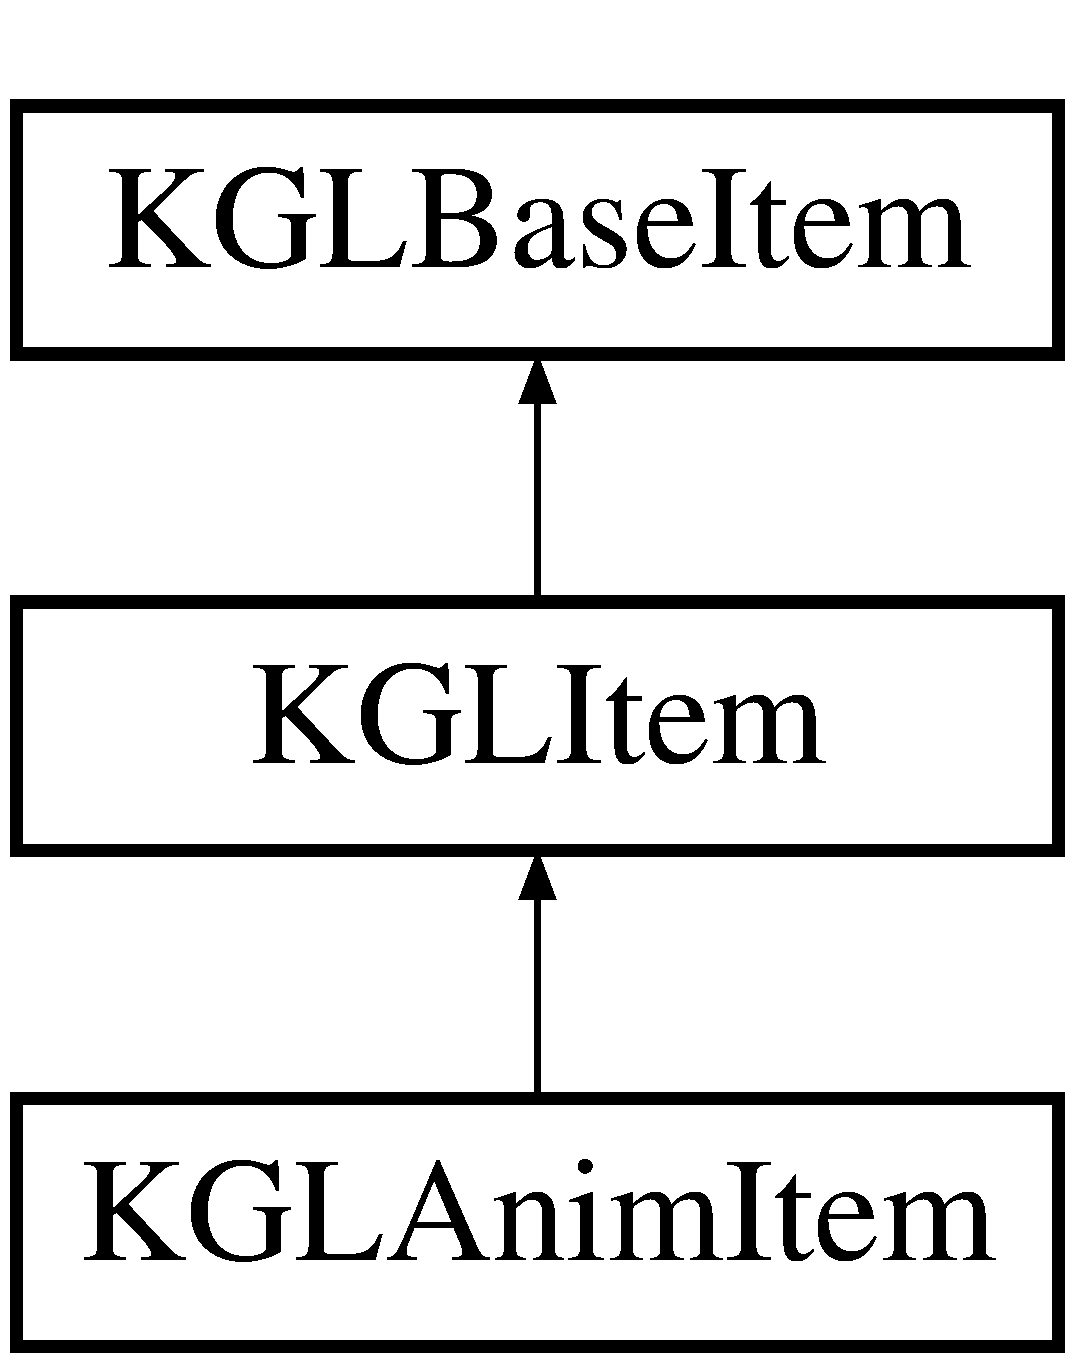
\includegraphics[height=3cm]{class_k_g_l_anim_item}
\end{center}
\end{figure}
\subsection*{Public Slots}
\begin{CompactItemize}
\item 
void \hyperlink{class_k_g_l_anim_item_6b61e41500543929dda03b741240cfb5}{createFrame} (int id=0)
\end{CompactItemize}
\subsection*{Public Member Functions}
\begin{CompactItemize}
\item 
\hyperlink{class_k_g_l_anim_item_59946ab271701727f87533abf1bde4f4}{KGLAnimItem} (const GLint \&texture, const int \&nbFrame=2, const int \&duration=500, const QSizeF \&dim=QSizeF(0.5, 0.5))
\end{CompactItemize}


\subsection{Constructor \& Destructor Documentation}
\hypertarget{class_k_g_l_anim_item_59946ab271701727f87533abf1bde4f4}{
\index{KGLAnimItem@{KGLAnimItem}!KGLAnimItem@{KGLAnimItem}}
\index{KGLAnimItem@{KGLAnimItem}!KGLAnimItem@{KGLAnimItem}}
\subsubsection[{KGLAnimItem}]{\setlength{\rightskip}{0pt plus 5cm}KGLAnimItem::KGLAnimItem (const GLint \& {\em texture}, \/  const int \& {\em nbFrame} = {\tt 2}, \/  const int \& {\em duration} = {\tt 500}, \/  const QSizeF \& {\em dim} = {\tt QSizeF(0.5,~0.5)})\hspace{0.3cm}{\tt  \mbox{[}explicit\mbox{]}}}}
\label{class_k_g_l_anim_item_59946ab271701727f87533abf1bde4f4}




\subsection{Member Function Documentation}
\hypertarget{class_k_g_l_anim_item_6b61e41500543929dda03b741240cfb5}{
\index{KGLAnimItem@{KGLAnimItem}!createFrame@{createFrame}}
\index{createFrame@{createFrame}!KGLAnimItem@{KGLAnimItem}}
\subsubsection[{createFrame}]{\setlength{\rightskip}{0pt plus 5cm}void KGLAnimItem::createFrame (int {\em id} = {\tt 0})\hspace{0.3cm}{\tt  \mbox{[}slot\mbox{]}}}}
\label{class_k_g_l_anim_item_6b61e41500543929dda03b741240cfb5}




The documentation for this class was generated from the following files:\begin{CompactItemize}
\item 
/home/sacha/programmation/gluon/kgl/\hyperlink{kglanimitem_8h}{kglanimitem.h}\item 
/home/sacha/programmation/gluon/kgl/\hyperlink{kglanimitem_8cpp}{kglanimitem.cpp}\end{CompactItemize}

\hypertarget{class_k_g_l_base_item}{
\section{KGLBaseItem Class Reference}
\label{class_k_g_l_base_item}\index{KGLBaseItem@{KGLBaseItem}}
}
{\tt \#include $<$kglbaseitem.h$>$}

Inheritance diagram for KGLBaseItem::\begin{figure}[H]
\begin{center}
\leavevmode
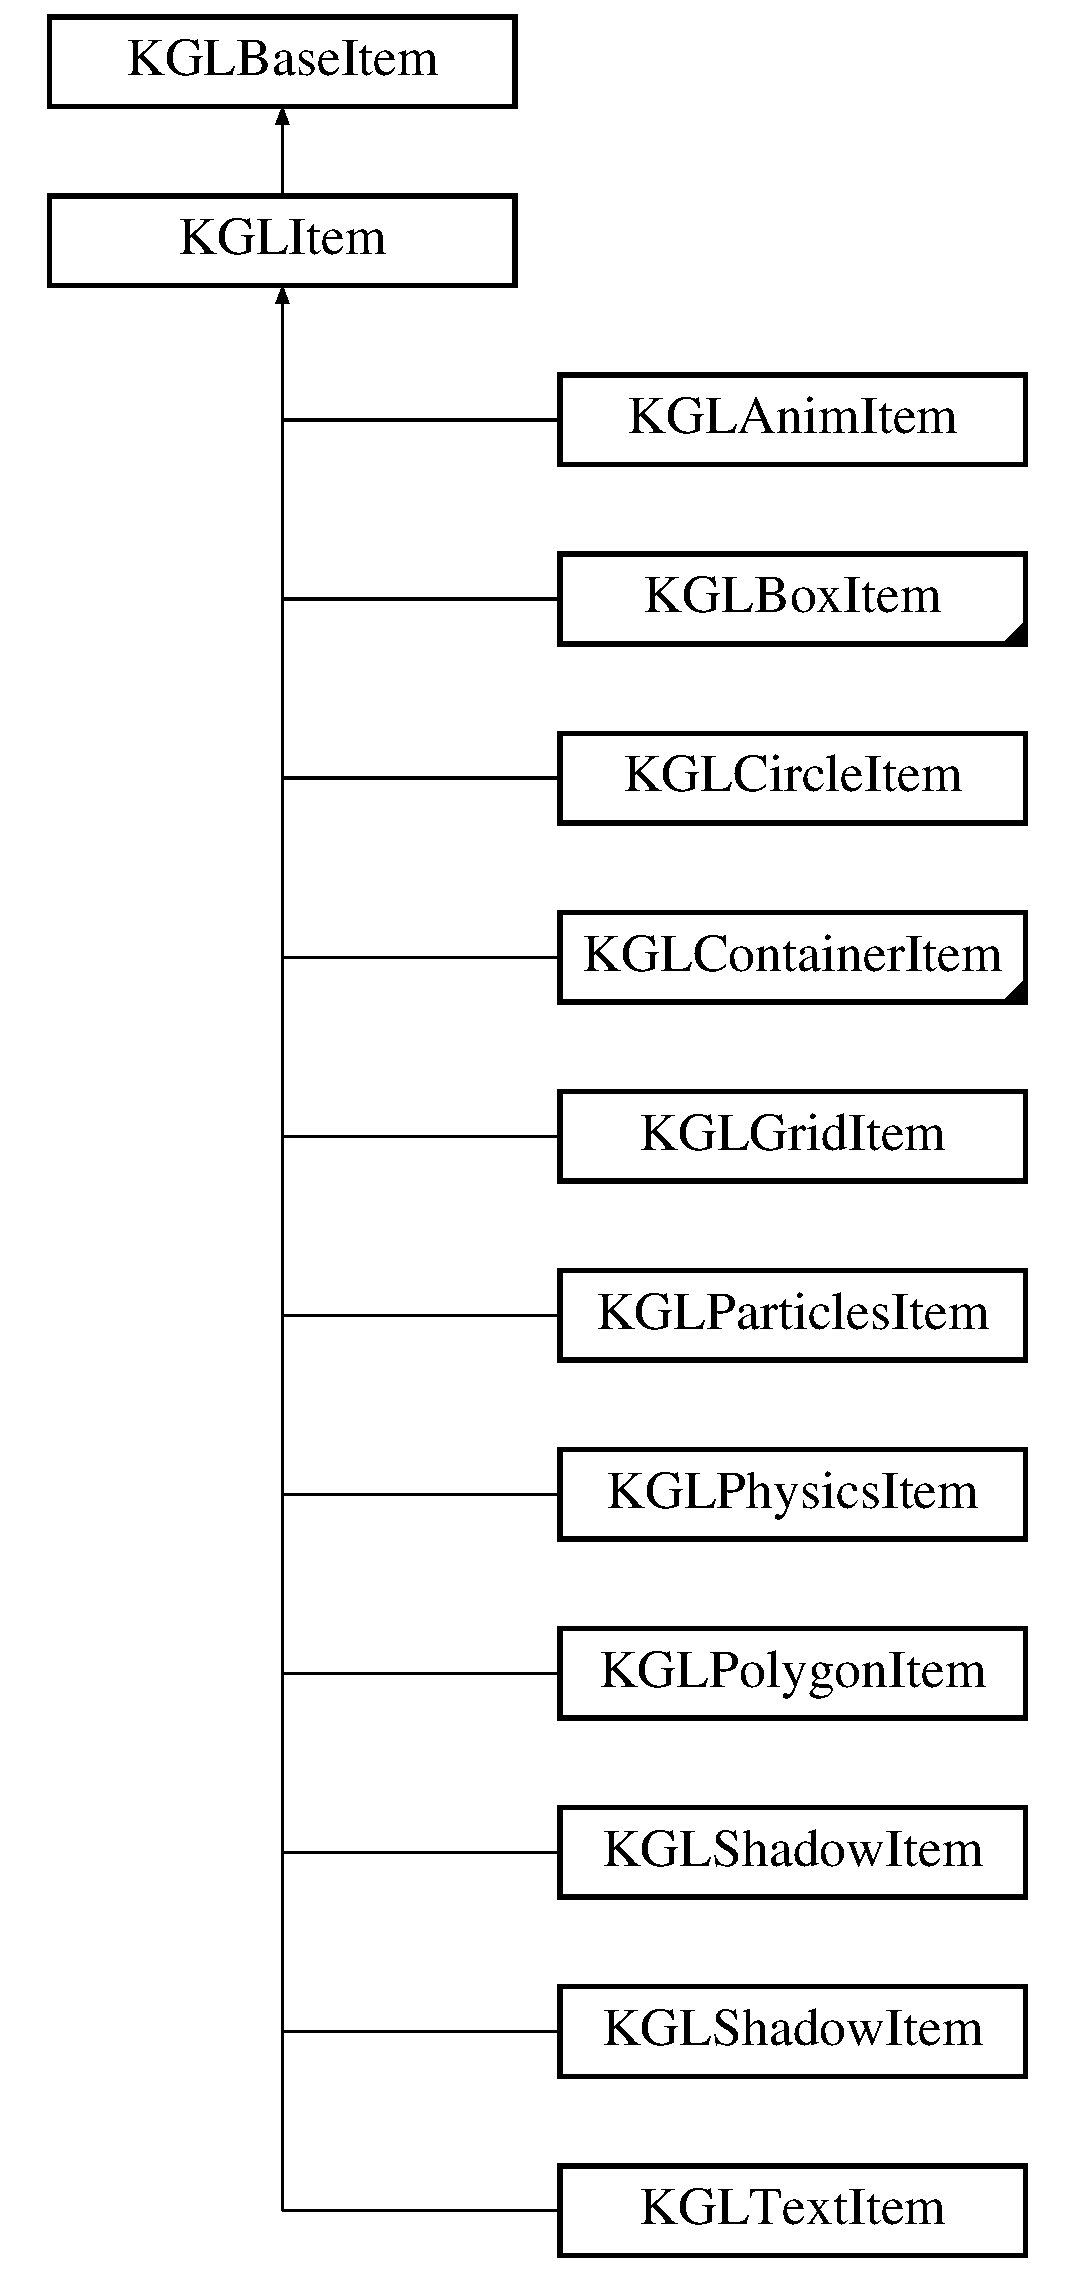
\includegraphics[height=12cm]{class_k_g_l_base_item}
\end{center}
\end{figure}
\subsection*{Public Member Functions}
\begin{CompactItemize}
\item 
\hyperlink{class_k_g_l_base_item_9743d8f5ce7ec1de26267c6d34bf6303}{KGLBaseItem} (QObject $\ast$parent=0)
\item 
\hyperlink{class_k_g_l_base_item_8aaeca0452e979304a98056441a14cdd}{$\sim$KGLBaseItem} ()
\item 
virtual void \hyperlink{class_k_g_l_base_item_3eabedeecf9e7b82d82557c95c56741a}{addVertex} (const \hyperlink{class_k_g_l_point}{KGLPoint} \&p)
\item 
\hyperlink{class_k_g_l_point_list}{KGLPointList} \& \hyperlink{class_k_g_l_base_item_83092e2126b730daf7d774630113bb66}{pointList} ()
\item 
virtual void \hyperlink{class_k_g_l_base_item_58c4e6cb39b23d5f313f425cf9afc99c}{removeVertex} (\hyperlink{class_k_g_l_point}{KGLPoint} $\ast$p)
\item 
virtual void \hyperlink{class_k_g_l_base_item_b84b10f4cbeeb352cf91f327a564b377}{clear} ()
\item 
virtual void \hyperlink{class_k_g_l_base_item_6e020830d4452864cdb6c8fea4531e0d}{updateTransform} ()
\item 
virtual void \hyperlink{class_k_g_l_base_item_5aa1d880fffcc82847dc7eff4e7aecba}{resetTransform} ()
\item 
void \hyperlink{class_k_g_l_base_item_49c808d884735aa2df77d8673c250535}{applyTransform} (const Eigen::Transform3d \&m)
\item 
void \hyperlink{class_k_g_l_base_item_180099829489993a95ec445a46ac49d3}{createBox} (const QSizeF \&s)
\item 
void \hyperlink{class_k_g_l_base_item_092dd2a3401a1192fecbf63c8a486777}{createBox} (const float \&w, const float \&h)
\item 
void \hyperlink{class_k_g_l_base_item_849ec6bf857c964042b8c2f1305fd5b1}{createPolygon} (const QPolygonF \&poly)
\item 
void \hyperlink{class_k_g_l_base_item_810379a4aac12d9061b14b2aa3e55ea6}{createLine} (const QLineF \&line)
\item 
unsigned int \hyperlink{class_k_g_l_base_item_22a498a5b8fdd0eb6ffcca48678a58a1}{pointCount} ()
\item 
const QPointF \& \hyperlink{class_k_g_l_base_item_40e86b4a2929ae6b230fb0764af53c3c}{position} ()
\item 
const float \& \hyperlink{class_k_g_l_base_item_eeb20ccf94f92b5813a291cd2436dd63}{scaleValue} ()
\item 
const float \& \hyperlink{class_k_g_l_base_item_e81d2c64201c36247fa1d0fda08052c6}{angle} ()
\item 
const float \& \hyperlink{class_k_g_l_base_item_80a9678e8406bdd261cea2aaa8d687a7}{radius} ()
\item 
unsigned int \hyperlink{class_k_g_l_base_item_22da0f3dbc3522a836980df6f8e96def}{zindex} ()
\item 
const QPointF \hyperlink{class_k_g_l_base_item_756267078e458ee97974bc610ff332b1}{center} ()
\item 
const QPointF \& \hyperlink{class_k_g_l_base_item_36470fb553034ab369b5d9349f2590ca}{itemCenter} ()
\item 
const QPolygonF \hyperlink{class_k_g_l_base_item_87a09a44afa6e73baa9aa6d30e81a163}{polygon} ()
\item 
const QPolygonF \hyperlink{class_k_g_l_base_item_9f428b73219decd7b0682db7baab258c}{itemPolygon} ()
\item 
virtual const QRectF \hyperlink{class_k_g_l_base_item_b0b84c51ad212eae0873afa956ace7cf}{boundingBox} ()
\item 
virtual const QRectF \hyperlink{class_k_g_l_base_item_0b12fe848be4194ccd67464d63ab4d25}{itemBoundingBox} ()
\item 
bool \hyperlink{class_k_g_l_base_item_d69c3373e2bc0d47881dff95456c1bbc}{contains} (QPointF \&p)
\item 
Eigen::Transform3d \& \hyperlink{class_k_g_l_base_item_a42b375ad542d3e64eb7aee95d9e6385}{matrix} ()
\item 
void \hyperlink{class_k_g_l_base_item_1897bc88d905d28ff05ac177c0619060}{setMatrix} (const Eigen::Transform3d \&m)
\item 
void \hyperlink{class_k_g_l_base_item_85c4af1445672402e3b47735e2bbf415}{setCenter} (const QPointF \&c)
\item 
void \hyperlink{class_k_g_l_base_item_a281df5a9d5d601635956268809bc67e}{setAngle} (const float \&a, QPointF c=QPointF(0, 0))
\item 
void \hyperlink{class_k_g_l_base_item_d3b52ffc2c83b762a2bd0d678215295e}{setScale} (const float \&s)
\item 
void \hyperlink{class_k_g_l_base_item_05ad2bc6e34005638626afda94f53269}{setPosition} (const QPointF \&p)
\item 
void \hyperlink{class_k_g_l_base_item_f9b1881b93773e84b1a2bd1483183d2e}{setPosition} (qreal x, qreal y)
\item 
void \hyperlink{class_k_g_l_base_item_c66fae31fcfb2261694c8ec120cb314c}{setShear} (const QPointF \&s)
\item 
void \hyperlink{class_k_g_l_base_item_19095252a25d1c9fdcf1950625ed81e4}{setShear} (const float \&sx, const float \&sy)
\item 
void \hyperlink{class_k_g_l_base_item_e29dcbe6e797fd4c6aef59acadb5ba48}{setZIndex} (int i)
\item 
void \hyperlink{class_k_g_l_base_item_a953c569ebcb00d8e9f8a7a88a730930}{translate} (const QPointF \&step)
\item 
void \hyperlink{class_k_g_l_base_item_69f7ca20cd192bd7ccc5bfdaeac4e60e}{translate} (const float \&x, const float \&y)
\item 
void \hyperlink{class_k_g_l_base_item_03c0cf1d821aebbe56d0a15681c17f1f}{scale} (const float \&s)
\item 
void \hyperlink{class_k_g_l_base_item_e3f4ea29b0d2da2a296ddbb80ea88738}{rotate} (const float \&angle)
\item 
void \hyperlink{class_k_g_l_base_item_a7cb811a03472f52dd7f6090a305bc30}{shear} (const QPointF \&s)
\item 
void \hyperlink{class_k_g_l_base_item_a81489bbb8b7ebe54129eab7b56d8b1a}{shear} (const float \&sx, const float \&sy)
\end{CompactItemize}
\subsection*{Protected Member Functions}
\begin{CompactItemize}
\item 
void \hyperlink{class_k_g_l_base_item_4fb2662f683c8d710039f229583c8c1c}{computeGeometry} ()
\item 
void \hyperlink{class_k_g_l_base_item_628f1737fb9ec96f4296798f86a2fcdb}{initShearMatrix} (QPointF s)
\item 
QPointF \hyperlink{class_k_g_l_base_item_3825639b143ff214e96749f375449675}{transform} (QPointF p)
\item 
QPolygonF \hyperlink{class_k_g_l_base_item_8df2be0816e3d24bf9adb5f0a01d186b}{transform} (QPolygonF p)
\item 
QRectF \hyperlink{class_k_g_l_base_item_fd255933afb0b5eb06de5ac1358f7e24}{transform} (QRectF r)
\end{CompactItemize}


\subsection{Constructor \& Destructor Documentation}
\hypertarget{class_k_g_l_base_item_9743d8f5ce7ec1de26267c6d34bf6303}{
\index{KGLBaseItem@{KGLBaseItem}!KGLBaseItem@{KGLBaseItem}}
\index{KGLBaseItem@{KGLBaseItem}!KGLBaseItem@{KGLBaseItem}}
\subsubsection[{KGLBaseItem}]{\setlength{\rightskip}{0pt plus 5cm}KGLBaseItem::KGLBaseItem (QObject $\ast$ {\em parent} = {\tt 0})}}
\label{class_k_g_l_base_item_9743d8f5ce7ec1de26267c6d34bf6303}


\hypertarget{class_k_g_l_base_item_8aaeca0452e979304a98056441a14cdd}{
\index{KGLBaseItem@{KGLBaseItem}!$\sim$KGLBaseItem@{$\sim$KGLBaseItem}}
\index{$\sim$KGLBaseItem@{$\sim$KGLBaseItem}!KGLBaseItem@{KGLBaseItem}}
\subsubsection[{$\sim$KGLBaseItem}]{\setlength{\rightskip}{0pt plus 5cm}KGLBaseItem::$\sim$KGLBaseItem ()}}
\label{class_k_g_l_base_item_8aaeca0452e979304a98056441a14cdd}




\subsection{Member Function Documentation}
\hypertarget{class_k_g_l_base_item_3eabedeecf9e7b82d82557c95c56741a}{
\index{KGLBaseItem@{KGLBaseItem}!addVertex@{addVertex}}
\index{addVertex@{addVertex}!KGLBaseItem@{KGLBaseItem}}
\subsubsection[{addVertex}]{\setlength{\rightskip}{0pt plus 5cm}virtual void KGLBaseItem::addVertex (const {\bf KGLPoint} \& {\em p})\hspace{0.3cm}{\tt  \mbox{[}inline, virtual\mbox{]}}}}
\label{class_k_g_l_base_item_3eabedeecf9e7b82d82557c95c56741a}


\hypertarget{class_k_g_l_base_item_e81d2c64201c36247fa1d0fda08052c6}{
\index{KGLBaseItem@{KGLBaseItem}!angle@{angle}}
\index{angle@{angle}!KGLBaseItem@{KGLBaseItem}}
\subsubsection[{angle}]{\setlength{\rightskip}{0pt plus 5cm}const float\& KGLBaseItem::angle ()\hspace{0.3cm}{\tt  \mbox{[}inline\mbox{]}}}}
\label{class_k_g_l_base_item_e81d2c64201c36247fa1d0fda08052c6}


\hypertarget{class_k_g_l_base_item_49c808d884735aa2df77d8673c250535}{
\index{KGLBaseItem@{KGLBaseItem}!applyTransform@{applyTransform}}
\index{applyTransform@{applyTransform}!KGLBaseItem@{KGLBaseItem}}
\subsubsection[{applyTransform}]{\setlength{\rightskip}{0pt plus 5cm}void KGLBaseItem::applyTransform (const Eigen::Transform3d \& {\em m})\hspace{0.3cm}{\tt  \mbox{[}inline\mbox{]}}}}
\label{class_k_g_l_base_item_49c808d884735aa2df77d8673c250535}


\hypertarget{class_k_g_l_base_item_b0b84c51ad212eae0873afa956ace7cf}{
\index{KGLBaseItem@{KGLBaseItem}!boundingBox@{boundingBox}}
\index{boundingBox@{boundingBox}!KGLBaseItem@{KGLBaseItem}}
\subsubsection[{boundingBox}]{\setlength{\rightskip}{0pt plus 5cm}virtual const QRectF KGLBaseItem::boundingBox ()\hspace{0.3cm}{\tt  \mbox{[}inline, virtual\mbox{]}}}}
\label{class_k_g_l_base_item_b0b84c51ad212eae0873afa956ace7cf}


\hypertarget{class_k_g_l_base_item_756267078e458ee97974bc610ff332b1}{
\index{KGLBaseItem@{KGLBaseItem}!center@{center}}
\index{center@{center}!KGLBaseItem@{KGLBaseItem}}
\subsubsection[{center}]{\setlength{\rightskip}{0pt plus 5cm}const QPointF KGLBaseItem::center ()\hspace{0.3cm}{\tt  \mbox{[}inline\mbox{]}}}}
\label{class_k_g_l_base_item_756267078e458ee97974bc610ff332b1}


\hypertarget{class_k_g_l_base_item_b84b10f4cbeeb352cf91f327a564b377}{
\index{KGLBaseItem@{KGLBaseItem}!clear@{clear}}
\index{clear@{clear}!KGLBaseItem@{KGLBaseItem}}
\subsubsection[{clear}]{\setlength{\rightskip}{0pt plus 5cm}virtual void KGLBaseItem::clear ()\hspace{0.3cm}{\tt  \mbox{[}inline, virtual\mbox{]}}}}
\label{class_k_g_l_base_item_b84b10f4cbeeb352cf91f327a564b377}


\hypertarget{class_k_g_l_base_item_4fb2662f683c8d710039f229583c8c1c}{
\index{KGLBaseItem@{KGLBaseItem}!computeGeometry@{computeGeometry}}
\index{computeGeometry@{computeGeometry}!KGLBaseItem@{KGLBaseItem}}
\subsubsection[{computeGeometry}]{\setlength{\rightskip}{0pt plus 5cm}void KGLBaseItem::computeGeometry ()\hspace{0.3cm}{\tt  \mbox{[}protected\mbox{]}}}}
\label{class_k_g_l_base_item_4fb2662f683c8d710039f229583c8c1c}


\hypertarget{class_k_g_l_base_item_d69c3373e2bc0d47881dff95456c1bbc}{
\index{KGLBaseItem@{KGLBaseItem}!contains@{contains}}
\index{contains@{contains}!KGLBaseItem@{KGLBaseItem}}
\subsubsection[{contains}]{\setlength{\rightskip}{0pt plus 5cm}bool KGLBaseItem::contains (QPointF \& {\em p})\hspace{0.3cm}{\tt  \mbox{[}inline\mbox{]}}}}
\label{class_k_g_l_base_item_d69c3373e2bc0d47881dff95456c1bbc}


\hypertarget{class_k_g_l_base_item_092dd2a3401a1192fecbf63c8a486777}{
\index{KGLBaseItem@{KGLBaseItem}!createBox@{createBox}}
\index{createBox@{createBox}!KGLBaseItem@{KGLBaseItem}}
\subsubsection[{createBox}]{\setlength{\rightskip}{0pt plus 5cm}void KGLBaseItem::createBox (const float \& {\em w}, \/  const float \& {\em h})\hspace{0.3cm}{\tt  \mbox{[}inline\mbox{]}}}}
\label{class_k_g_l_base_item_092dd2a3401a1192fecbf63c8a486777}


\hypertarget{class_k_g_l_base_item_180099829489993a95ec445a46ac49d3}{
\index{KGLBaseItem@{KGLBaseItem}!createBox@{createBox}}
\index{createBox@{createBox}!KGLBaseItem@{KGLBaseItem}}
\subsubsection[{createBox}]{\setlength{\rightskip}{0pt plus 5cm}void KGLBaseItem::createBox (const QSizeF \& {\em s})}}
\label{class_k_g_l_base_item_180099829489993a95ec445a46ac49d3}


\hypertarget{class_k_g_l_base_item_810379a4aac12d9061b14b2aa3e55ea6}{
\index{KGLBaseItem@{KGLBaseItem}!createLine@{createLine}}
\index{createLine@{createLine}!KGLBaseItem@{KGLBaseItem}}
\subsubsection[{createLine}]{\setlength{\rightskip}{0pt plus 5cm}void KGLBaseItem::createLine (const QLineF \& {\em line})}}
\label{class_k_g_l_base_item_810379a4aac12d9061b14b2aa3e55ea6}


\hypertarget{class_k_g_l_base_item_849ec6bf857c964042b8c2f1305fd5b1}{
\index{KGLBaseItem@{KGLBaseItem}!createPolygon@{createPolygon}}
\index{createPolygon@{createPolygon}!KGLBaseItem@{KGLBaseItem}}
\subsubsection[{createPolygon}]{\setlength{\rightskip}{0pt plus 5cm}void KGLBaseItem::createPolygon (const QPolygonF \& {\em poly})}}
\label{class_k_g_l_base_item_849ec6bf857c964042b8c2f1305fd5b1}


\hypertarget{class_k_g_l_base_item_628f1737fb9ec96f4296798f86a2fcdb}{
\index{KGLBaseItem@{KGLBaseItem}!initShearMatrix@{initShearMatrix}}
\index{initShearMatrix@{initShearMatrix}!KGLBaseItem@{KGLBaseItem}}
\subsubsection[{initShearMatrix}]{\setlength{\rightskip}{0pt plus 5cm}void KGLBaseItem::initShearMatrix (QPointF {\em s})\hspace{0.3cm}{\tt  \mbox{[}protected\mbox{]}}}}
\label{class_k_g_l_base_item_628f1737fb9ec96f4296798f86a2fcdb}


\hypertarget{class_k_g_l_base_item_0b12fe848be4194ccd67464d63ab4d25}{
\index{KGLBaseItem@{KGLBaseItem}!itemBoundingBox@{itemBoundingBox}}
\index{itemBoundingBox@{itemBoundingBox}!KGLBaseItem@{KGLBaseItem}}
\subsubsection[{itemBoundingBox}]{\setlength{\rightskip}{0pt plus 5cm}virtual const QRectF KGLBaseItem::itemBoundingBox ()\hspace{0.3cm}{\tt  \mbox{[}inline, virtual\mbox{]}}}}
\label{class_k_g_l_base_item_0b12fe848be4194ccd67464d63ab4d25}


\hypertarget{class_k_g_l_base_item_36470fb553034ab369b5d9349f2590ca}{
\index{KGLBaseItem@{KGLBaseItem}!itemCenter@{itemCenter}}
\index{itemCenter@{itemCenter}!KGLBaseItem@{KGLBaseItem}}
\subsubsection[{itemCenter}]{\setlength{\rightskip}{0pt plus 5cm}const QPointF\& KGLBaseItem::itemCenter ()\hspace{0.3cm}{\tt  \mbox{[}inline\mbox{]}}}}
\label{class_k_g_l_base_item_36470fb553034ab369b5d9349f2590ca}


\hypertarget{class_k_g_l_base_item_9f428b73219decd7b0682db7baab258c}{
\index{KGLBaseItem@{KGLBaseItem}!itemPolygon@{itemPolygon}}
\index{itemPolygon@{itemPolygon}!KGLBaseItem@{KGLBaseItem}}
\subsubsection[{itemPolygon}]{\setlength{\rightskip}{0pt plus 5cm}const QPolygonF KGLBaseItem::itemPolygon ()\hspace{0.3cm}{\tt  \mbox{[}inline\mbox{]}}}}
\label{class_k_g_l_base_item_9f428b73219decd7b0682db7baab258c}


\hypertarget{class_k_g_l_base_item_a42b375ad542d3e64eb7aee95d9e6385}{
\index{KGLBaseItem@{KGLBaseItem}!matrix@{matrix}}
\index{matrix@{matrix}!KGLBaseItem@{KGLBaseItem}}
\subsubsection[{matrix}]{\setlength{\rightskip}{0pt plus 5cm}Eigen::Transform3d\& KGLBaseItem::matrix ()\hspace{0.3cm}{\tt  \mbox{[}inline\mbox{]}}}}
\label{class_k_g_l_base_item_a42b375ad542d3e64eb7aee95d9e6385}


\hypertarget{class_k_g_l_base_item_22a498a5b8fdd0eb6ffcca48678a58a1}{
\index{KGLBaseItem@{KGLBaseItem}!pointCount@{pointCount}}
\index{pointCount@{pointCount}!KGLBaseItem@{KGLBaseItem}}
\subsubsection[{pointCount}]{\setlength{\rightskip}{0pt plus 5cm}unsigned int KGLBaseItem::pointCount ()\hspace{0.3cm}{\tt  \mbox{[}inline\mbox{]}}}}
\label{class_k_g_l_base_item_22a498a5b8fdd0eb6ffcca48678a58a1}


\hypertarget{class_k_g_l_base_item_83092e2126b730daf7d774630113bb66}{
\index{KGLBaseItem@{KGLBaseItem}!pointList@{pointList}}
\index{pointList@{pointList}!KGLBaseItem@{KGLBaseItem}}
\subsubsection[{pointList}]{\setlength{\rightskip}{0pt plus 5cm}{\bf KGLPointList}\& KGLBaseItem::pointList ()\hspace{0.3cm}{\tt  \mbox{[}inline\mbox{]}}}}
\label{class_k_g_l_base_item_83092e2126b730daf7d774630113bb66}


\hypertarget{class_k_g_l_base_item_87a09a44afa6e73baa9aa6d30e81a163}{
\index{KGLBaseItem@{KGLBaseItem}!polygon@{polygon}}
\index{polygon@{polygon}!KGLBaseItem@{KGLBaseItem}}
\subsubsection[{polygon}]{\setlength{\rightskip}{0pt plus 5cm}const QPolygonF KGLBaseItem::polygon ()\hspace{0.3cm}{\tt  \mbox{[}inline\mbox{]}}}}
\label{class_k_g_l_base_item_87a09a44afa6e73baa9aa6d30e81a163}


\hypertarget{class_k_g_l_base_item_40e86b4a2929ae6b230fb0764af53c3c}{
\index{KGLBaseItem@{KGLBaseItem}!position@{position}}
\index{position@{position}!KGLBaseItem@{KGLBaseItem}}
\subsubsection[{position}]{\setlength{\rightskip}{0pt plus 5cm}const QPointF\& KGLBaseItem::position ()\hspace{0.3cm}{\tt  \mbox{[}inline\mbox{]}}}}
\label{class_k_g_l_base_item_40e86b4a2929ae6b230fb0764af53c3c}


\hypertarget{class_k_g_l_base_item_80a9678e8406bdd261cea2aaa8d687a7}{
\index{KGLBaseItem@{KGLBaseItem}!radius@{radius}}
\index{radius@{radius}!KGLBaseItem@{KGLBaseItem}}
\subsubsection[{radius}]{\setlength{\rightskip}{0pt plus 5cm}const float\& KGLBaseItem::radius ()\hspace{0.3cm}{\tt  \mbox{[}inline\mbox{]}}}}
\label{class_k_g_l_base_item_80a9678e8406bdd261cea2aaa8d687a7}


\hypertarget{class_k_g_l_base_item_58c4e6cb39b23d5f313f425cf9afc99c}{
\index{KGLBaseItem@{KGLBaseItem}!removeVertex@{removeVertex}}
\index{removeVertex@{removeVertex}!KGLBaseItem@{KGLBaseItem}}
\subsubsection[{removeVertex}]{\setlength{\rightskip}{0pt plus 5cm}virtual void KGLBaseItem::removeVertex ({\bf KGLPoint} $\ast$ {\em p})\hspace{0.3cm}{\tt  \mbox{[}inline, virtual\mbox{]}}}}
\label{class_k_g_l_base_item_58c4e6cb39b23d5f313f425cf9afc99c}


\hypertarget{class_k_g_l_base_item_5aa1d880fffcc82847dc7eff4e7aecba}{
\index{KGLBaseItem@{KGLBaseItem}!resetTransform@{resetTransform}}
\index{resetTransform@{resetTransform}!KGLBaseItem@{KGLBaseItem}}
\subsubsection[{resetTransform}]{\setlength{\rightskip}{0pt plus 5cm}void KGLBaseItem::resetTransform ()\hspace{0.3cm}{\tt  \mbox{[}virtual\mbox{]}}}}
\label{class_k_g_l_base_item_5aa1d880fffcc82847dc7eff4e7aecba}


\hypertarget{class_k_g_l_base_item_e3f4ea29b0d2da2a296ddbb80ea88738}{
\index{KGLBaseItem@{KGLBaseItem}!rotate@{rotate}}
\index{rotate@{rotate}!KGLBaseItem@{KGLBaseItem}}
\subsubsection[{rotate}]{\setlength{\rightskip}{0pt plus 5cm}void KGLBaseItem::rotate (const float \& {\em angle})\hspace{0.3cm}{\tt  \mbox{[}inline\mbox{]}}}}
\label{class_k_g_l_base_item_e3f4ea29b0d2da2a296ddbb80ea88738}


\hypertarget{class_k_g_l_base_item_03c0cf1d821aebbe56d0a15681c17f1f}{
\index{KGLBaseItem@{KGLBaseItem}!scale@{scale}}
\index{scale@{scale}!KGLBaseItem@{KGLBaseItem}}
\subsubsection[{scale}]{\setlength{\rightskip}{0pt plus 5cm}void KGLBaseItem::scale (const float \& {\em s})\hspace{0.3cm}{\tt  \mbox{[}inline\mbox{]}}}}
\label{class_k_g_l_base_item_03c0cf1d821aebbe56d0a15681c17f1f}


\hypertarget{class_k_g_l_base_item_eeb20ccf94f92b5813a291cd2436dd63}{
\index{KGLBaseItem@{KGLBaseItem}!scaleValue@{scaleValue}}
\index{scaleValue@{scaleValue}!KGLBaseItem@{KGLBaseItem}}
\subsubsection[{scaleValue}]{\setlength{\rightskip}{0pt plus 5cm}const float\& KGLBaseItem::scaleValue ()\hspace{0.3cm}{\tt  \mbox{[}inline\mbox{]}}}}
\label{class_k_g_l_base_item_eeb20ccf94f92b5813a291cd2436dd63}


\hypertarget{class_k_g_l_base_item_a281df5a9d5d601635956268809bc67e}{
\index{KGLBaseItem@{KGLBaseItem}!setAngle@{setAngle}}
\index{setAngle@{setAngle}!KGLBaseItem@{KGLBaseItem}}
\subsubsection[{setAngle}]{\setlength{\rightskip}{0pt plus 5cm}void KGLBaseItem::setAngle (const float \& {\em a}, \/  QPointF {\em c} = {\tt QPointF(0,0)})\hspace{0.3cm}{\tt  \mbox{[}inline\mbox{]}}}}
\label{class_k_g_l_base_item_a281df5a9d5d601635956268809bc67e}


\hypertarget{class_k_g_l_base_item_85c4af1445672402e3b47735e2bbf415}{
\index{KGLBaseItem@{KGLBaseItem}!setCenter@{setCenter}}
\index{setCenter@{setCenter}!KGLBaseItem@{KGLBaseItem}}
\subsubsection[{setCenter}]{\setlength{\rightskip}{0pt plus 5cm}void KGLBaseItem::setCenter (const QPointF \& {\em c})\hspace{0.3cm}{\tt  \mbox{[}inline\mbox{]}}}}
\label{class_k_g_l_base_item_85c4af1445672402e3b47735e2bbf415}


\hypertarget{class_k_g_l_base_item_1897bc88d905d28ff05ac177c0619060}{
\index{KGLBaseItem@{KGLBaseItem}!setMatrix@{setMatrix}}
\index{setMatrix@{setMatrix}!KGLBaseItem@{KGLBaseItem}}
\subsubsection[{setMatrix}]{\setlength{\rightskip}{0pt plus 5cm}void KGLBaseItem::setMatrix (const Eigen::Transform3d \& {\em m})\hspace{0.3cm}{\tt  \mbox{[}inline\mbox{]}}}}
\label{class_k_g_l_base_item_1897bc88d905d28ff05ac177c0619060}


\hypertarget{class_k_g_l_base_item_f9b1881b93773e84b1a2bd1483183d2e}{
\index{KGLBaseItem@{KGLBaseItem}!setPosition@{setPosition}}
\index{setPosition@{setPosition}!KGLBaseItem@{KGLBaseItem}}
\subsubsection[{setPosition}]{\setlength{\rightskip}{0pt plus 5cm}void KGLBaseItem::setPosition (qreal {\em x}, \/  qreal {\em y})\hspace{0.3cm}{\tt  \mbox{[}inline\mbox{]}}}}
\label{class_k_g_l_base_item_f9b1881b93773e84b1a2bd1483183d2e}


\hypertarget{class_k_g_l_base_item_05ad2bc6e34005638626afda94f53269}{
\index{KGLBaseItem@{KGLBaseItem}!setPosition@{setPosition}}
\index{setPosition@{setPosition}!KGLBaseItem@{KGLBaseItem}}
\subsubsection[{setPosition}]{\setlength{\rightskip}{0pt plus 5cm}void KGLBaseItem::setPosition (const QPointF \& {\em p})\hspace{0.3cm}{\tt  \mbox{[}inline\mbox{]}}}}
\label{class_k_g_l_base_item_05ad2bc6e34005638626afda94f53269}


\hypertarget{class_k_g_l_base_item_d3b52ffc2c83b762a2bd0d678215295e}{
\index{KGLBaseItem@{KGLBaseItem}!setScale@{setScale}}
\index{setScale@{setScale}!KGLBaseItem@{KGLBaseItem}}
\subsubsection[{setScale}]{\setlength{\rightskip}{0pt plus 5cm}void KGLBaseItem::setScale (const float \& {\em s})\hspace{0.3cm}{\tt  \mbox{[}inline\mbox{]}}}}
\label{class_k_g_l_base_item_d3b52ffc2c83b762a2bd0d678215295e}


\hypertarget{class_k_g_l_base_item_19095252a25d1c9fdcf1950625ed81e4}{
\index{KGLBaseItem@{KGLBaseItem}!setShear@{setShear}}
\index{setShear@{setShear}!KGLBaseItem@{KGLBaseItem}}
\subsubsection[{setShear}]{\setlength{\rightskip}{0pt plus 5cm}void KGLBaseItem::setShear (const float \& {\em sx}, \/  const float \& {\em sy})\hspace{0.3cm}{\tt  \mbox{[}inline\mbox{]}}}}
\label{class_k_g_l_base_item_19095252a25d1c9fdcf1950625ed81e4}


\hypertarget{class_k_g_l_base_item_c66fae31fcfb2261694c8ec120cb314c}{
\index{KGLBaseItem@{KGLBaseItem}!setShear@{setShear}}
\index{setShear@{setShear}!KGLBaseItem@{KGLBaseItem}}
\subsubsection[{setShear}]{\setlength{\rightskip}{0pt plus 5cm}void KGLBaseItem::setShear (const QPointF \& {\em s})\hspace{0.3cm}{\tt  \mbox{[}inline\mbox{]}}}}
\label{class_k_g_l_base_item_c66fae31fcfb2261694c8ec120cb314c}


\hypertarget{class_k_g_l_base_item_e29dcbe6e797fd4c6aef59acadb5ba48}{
\index{KGLBaseItem@{KGLBaseItem}!setZIndex@{setZIndex}}
\index{setZIndex@{setZIndex}!KGLBaseItem@{KGLBaseItem}}
\subsubsection[{setZIndex}]{\setlength{\rightskip}{0pt plus 5cm}void KGLBaseItem::setZIndex (int {\em i})\hspace{0.3cm}{\tt  \mbox{[}inline\mbox{]}}}}
\label{class_k_g_l_base_item_e29dcbe6e797fd4c6aef59acadb5ba48}


\hypertarget{class_k_g_l_base_item_a81489bbb8b7ebe54129eab7b56d8b1a}{
\index{KGLBaseItem@{KGLBaseItem}!shear@{shear}}
\index{shear@{shear}!KGLBaseItem@{KGLBaseItem}}
\subsubsection[{shear}]{\setlength{\rightskip}{0pt plus 5cm}void KGLBaseItem::shear (const float \& {\em sx}, \/  const float \& {\em sy})\hspace{0.3cm}{\tt  \mbox{[}inline\mbox{]}}}}
\label{class_k_g_l_base_item_a81489bbb8b7ebe54129eab7b56d8b1a}


\hypertarget{class_k_g_l_base_item_a7cb811a03472f52dd7f6090a305bc30}{
\index{KGLBaseItem@{KGLBaseItem}!shear@{shear}}
\index{shear@{shear}!KGLBaseItem@{KGLBaseItem}}
\subsubsection[{shear}]{\setlength{\rightskip}{0pt plus 5cm}void KGLBaseItem::shear (const QPointF \& {\em s})\hspace{0.3cm}{\tt  \mbox{[}inline\mbox{]}}}}
\label{class_k_g_l_base_item_a7cb811a03472f52dd7f6090a305bc30}


\hypertarget{class_k_g_l_base_item_fd255933afb0b5eb06de5ac1358f7e24}{
\index{KGLBaseItem@{KGLBaseItem}!transform@{transform}}
\index{transform@{transform}!KGLBaseItem@{KGLBaseItem}}
\subsubsection[{transform}]{\setlength{\rightskip}{0pt plus 5cm}QRectF KGLBaseItem::transform (QRectF {\em r})\hspace{0.3cm}{\tt  \mbox{[}protected\mbox{]}}}}
\label{class_k_g_l_base_item_fd255933afb0b5eb06de5ac1358f7e24}


\hypertarget{class_k_g_l_base_item_8df2be0816e3d24bf9adb5f0a01d186b}{
\index{KGLBaseItem@{KGLBaseItem}!transform@{transform}}
\index{transform@{transform}!KGLBaseItem@{KGLBaseItem}}
\subsubsection[{transform}]{\setlength{\rightskip}{0pt plus 5cm}QPolygonF KGLBaseItem::transform (QPolygonF {\em p})\hspace{0.3cm}{\tt  \mbox{[}protected\mbox{]}}}}
\label{class_k_g_l_base_item_8df2be0816e3d24bf9adb5f0a01d186b}


\hypertarget{class_k_g_l_base_item_3825639b143ff214e96749f375449675}{
\index{KGLBaseItem@{KGLBaseItem}!transform@{transform}}
\index{transform@{transform}!KGLBaseItem@{KGLBaseItem}}
\subsubsection[{transform}]{\setlength{\rightskip}{0pt plus 5cm}QPointF KGLBaseItem::transform (QPointF {\em p})\hspace{0.3cm}{\tt  \mbox{[}protected\mbox{]}}}}
\label{class_k_g_l_base_item_3825639b143ff214e96749f375449675}


\hypertarget{class_k_g_l_base_item_69f7ca20cd192bd7ccc5bfdaeac4e60e}{
\index{KGLBaseItem@{KGLBaseItem}!translate@{translate}}
\index{translate@{translate}!KGLBaseItem@{KGLBaseItem}}
\subsubsection[{translate}]{\setlength{\rightskip}{0pt plus 5cm}void KGLBaseItem::translate (const float \& {\em x}, \/  const float \& {\em y})\hspace{0.3cm}{\tt  \mbox{[}inline\mbox{]}}}}
\label{class_k_g_l_base_item_69f7ca20cd192bd7ccc5bfdaeac4e60e}


\hypertarget{class_k_g_l_base_item_a953c569ebcb00d8e9f8a7a88a730930}{
\index{KGLBaseItem@{KGLBaseItem}!translate@{translate}}
\index{translate@{translate}!KGLBaseItem@{KGLBaseItem}}
\subsubsection[{translate}]{\setlength{\rightskip}{0pt plus 5cm}void KGLBaseItem::translate (const QPointF \& {\em step})\hspace{0.3cm}{\tt  \mbox{[}inline\mbox{]}}}}
\label{class_k_g_l_base_item_a953c569ebcb00d8e9f8a7a88a730930}


\hypertarget{class_k_g_l_base_item_6e020830d4452864cdb6c8fea4531e0d}{
\index{KGLBaseItem@{KGLBaseItem}!updateTransform@{updateTransform}}
\index{updateTransform@{updateTransform}!KGLBaseItem@{KGLBaseItem}}
\subsubsection[{updateTransform}]{\setlength{\rightskip}{0pt plus 5cm}void KGLBaseItem::updateTransform ()\hspace{0.3cm}{\tt  \mbox{[}virtual\mbox{]}}}}
\label{class_k_g_l_base_item_6e020830d4452864cdb6c8fea4531e0d}




Reimplemented in \hyperlink{class_k_g_l_item_3dbecc9db8e526a4c9623b35a004ed3c}{KGLItem}.\hypertarget{class_k_g_l_base_item_22da0f3dbc3522a836980df6f8e96def}{
\index{KGLBaseItem@{KGLBaseItem}!zindex@{zindex}}
\index{zindex@{zindex}!KGLBaseItem@{KGLBaseItem}}
\subsubsection[{zindex}]{\setlength{\rightskip}{0pt plus 5cm}unsigned int KGLBaseItem::zindex ()\hspace{0.3cm}{\tt  \mbox{[}inline\mbox{]}}}}
\label{class_k_g_l_base_item_22da0f3dbc3522a836980df6f8e96def}




The documentation for this class was generated from the following files:\begin{CompactItemize}
\item 
/home/sacha/programmation/gluon/kgl/\hyperlink{kglbaseitem_8h}{kglbaseitem.h}\item 
/home/sacha/programmation/gluon/kgl/\hyperlink{kglbaseitem_8cpp}{kglbaseitem.cpp}\end{CompactItemize}

\hypertarget{class_k_g_l_blur_fx}{
\section{KGLBlurFx Class Reference}
\label{class_k_g_l_blur_fx}\index{KGLBlurFx@{KGLBlurFx}}
}
{\tt \#include $<$kglfx.h$>$}

Inheritance diagram for KGLBlurFx::\begin{figure}[H]
\begin{center}
\leavevmode
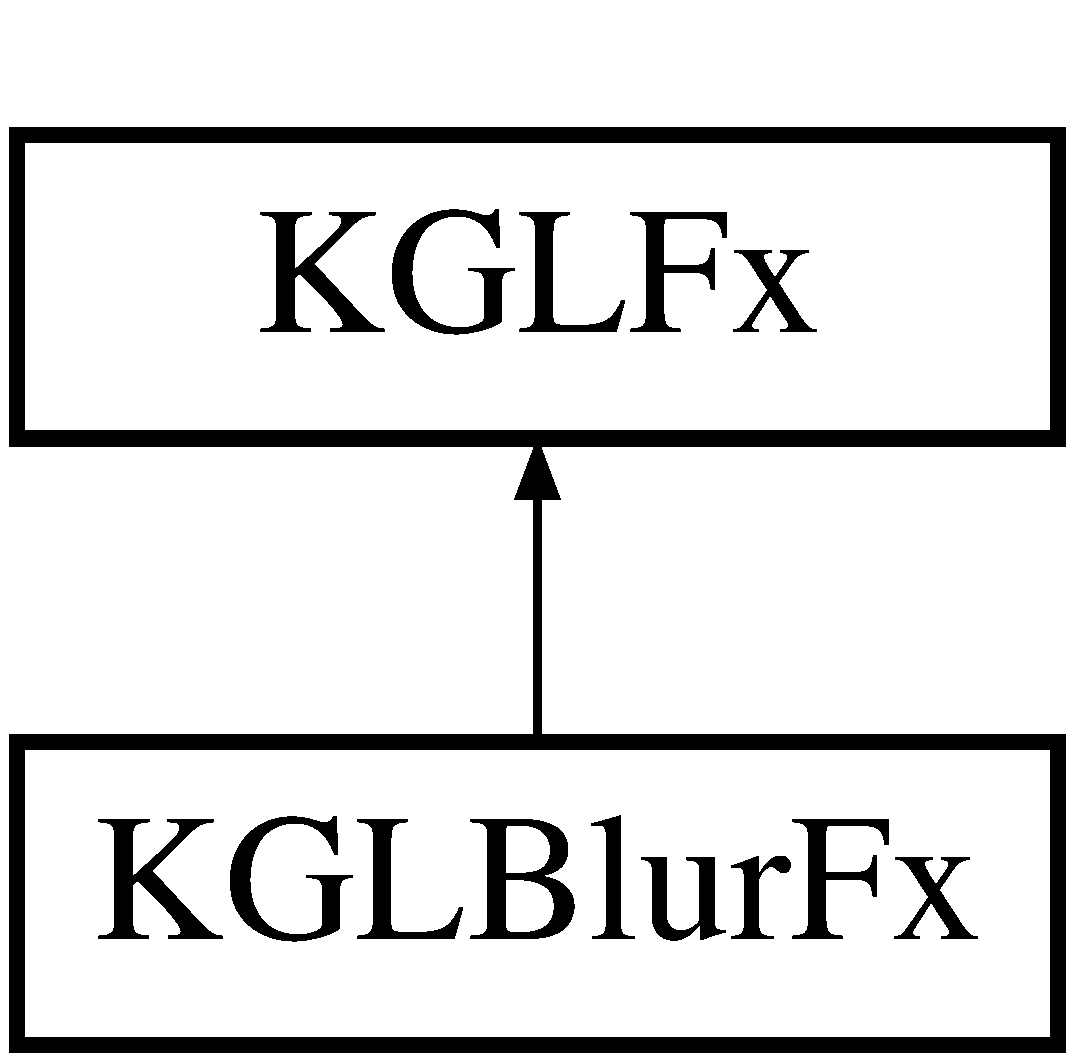
\includegraphics[height=2cm]{class_k_g_l_blur_fx}
\end{center}
\end{figure}
\subsection*{Public Member Functions}
\begin{CompactItemize}
\item 
\hyperlink{class_k_g_l_blur_fx_9d36e6a50c511834d83986055cc41cb4}{KGLBlurFx} ()
\item 
void \hyperlink{class_k_g_l_blur_fx_20e5761413ba19286c3d5484a4d37968}{setBlur} (float b)
\end{CompactItemize}


\subsection{Constructor \& Destructor Documentation}
\hypertarget{class_k_g_l_blur_fx_9d36e6a50c511834d83986055cc41cb4}{
\index{KGLBlurFx@{KGLBlurFx}!KGLBlurFx@{KGLBlurFx}}
\index{KGLBlurFx@{KGLBlurFx}!KGLBlurFx@{KGLBlurFx}}
\subsubsection[{KGLBlurFx}]{\setlength{\rightskip}{0pt plus 5cm}KGLBlurFx::KGLBlurFx ()}}
\label{class_k_g_l_blur_fx_9d36e6a50c511834d83986055cc41cb4}




\subsection{Member Function Documentation}
\hypertarget{class_k_g_l_blur_fx_20e5761413ba19286c3d5484a4d37968}{
\index{KGLBlurFx@{KGLBlurFx}!setBlur@{setBlur}}
\index{setBlur@{setBlur}!KGLBlurFx@{KGLBlurFx}}
\subsubsection[{setBlur}]{\setlength{\rightskip}{0pt plus 5cm}void KGLBlurFx::setBlur (float {\em b})\hspace{0.3cm}{\tt  \mbox{[}inline\mbox{]}}}}
\label{class_k_g_l_blur_fx_20e5761413ba19286c3d5484a4d37968}




The documentation for this class was generated from the following files:\begin{CompactItemize}
\item 
/home/sacha/programmation/gluon/kgl/\hyperlink{kglfx_8h}{kglfx.h}\item 
/home/sacha/programmation/gluon/kgl/\hyperlink{kglfx_8cpp}{kglfx.cpp}\end{CompactItemize}

\hypertarget{class_k_g_l_box_item}{
\section{KGLBoxItem Class Reference}
\label{class_k_g_l_box_item}\index{KGLBoxItem@{KGLBoxItem}}
}
{\tt \#include $<$KGLBoxItem$>$}

Inheritance diagram for KGLBoxItem::\begin{figure}[H]
\begin{center}
\leavevmode
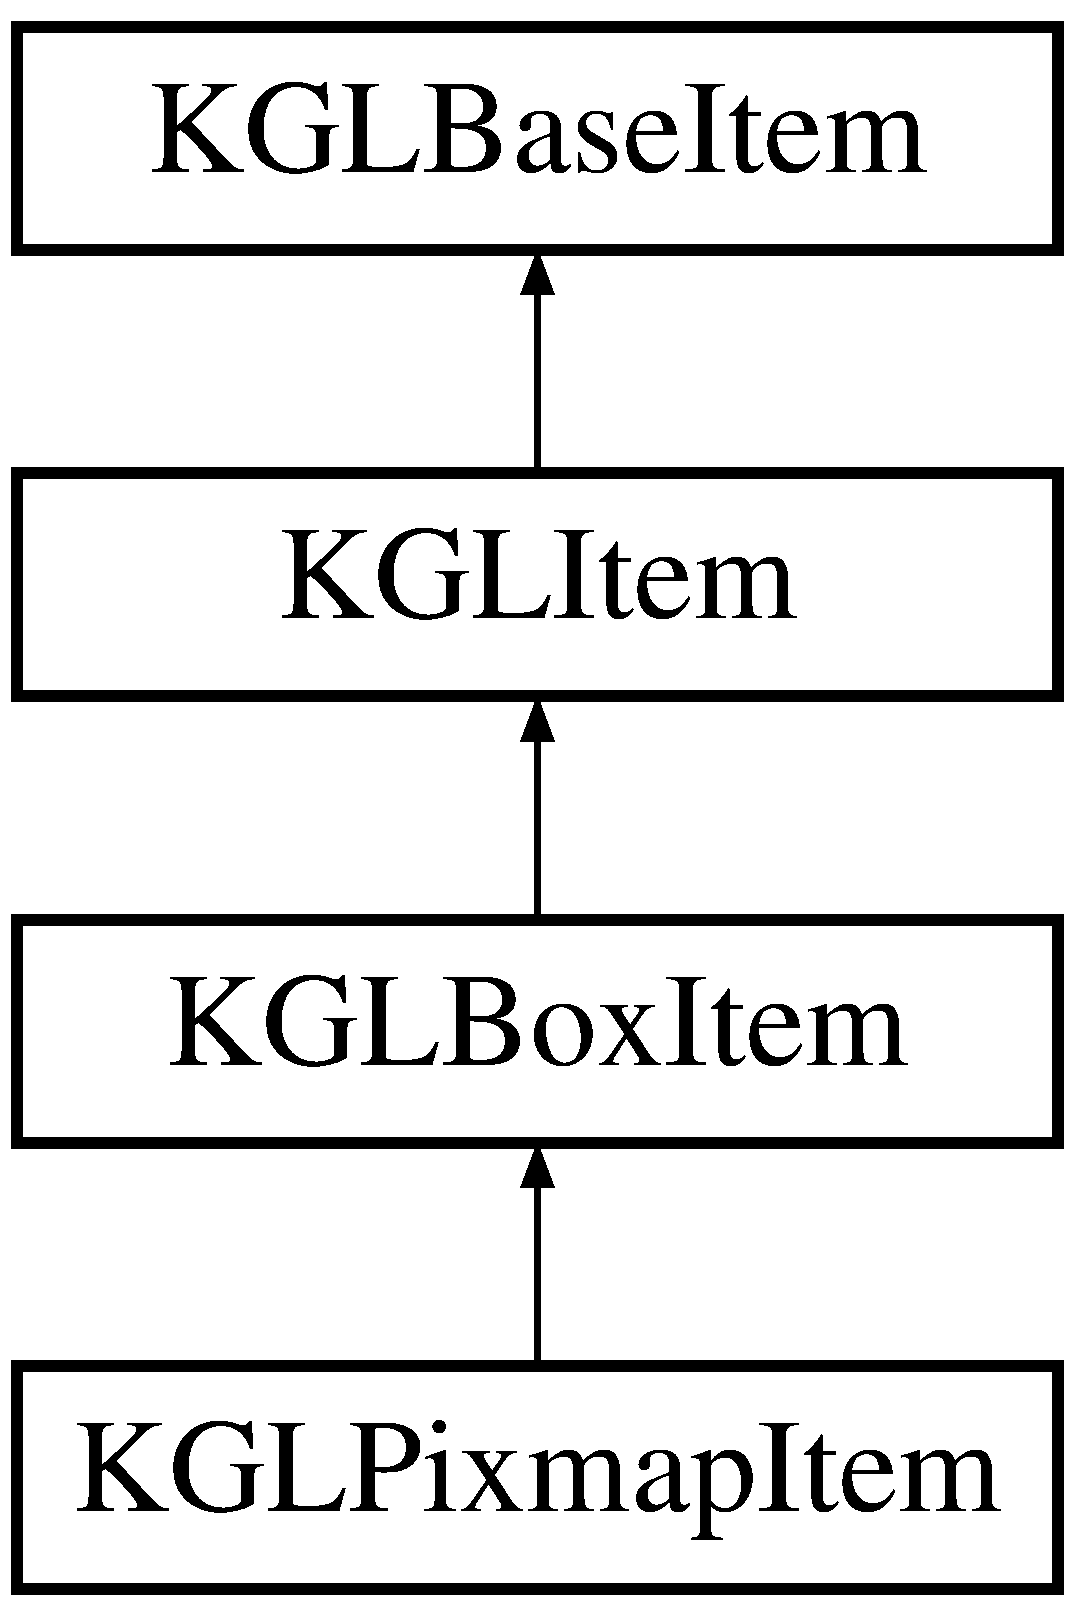
\includegraphics[height=4cm]{class_k_g_l_box_item}
\end{center}
\end{figure}
\subsection*{Public Member Functions}
\begin{CompactItemize}
\item 
\hyperlink{class_k_g_l_box_item_5c992045e6437b80c34fad9ac41f7dcc}{KGLBoxItem} (\hyperlink{class_k_g_l_engine}{KGLEngine} $\ast$parent=0)
\item 
\hyperlink{class_k_g_l_box_item_a9007cf09702c340fa0b8b5a38316977}{KGLBoxItem} (const QSizeF \&dim, \hyperlink{class_k_g_l_engine}{KGLEngine} $\ast$parent=0)
\item 
\hyperlink{class_k_g_l_box_item_e8f3c118be13227998e02c7bf52bb2e1}{KGLBoxItem} (const float \&w, const float \&h, \hyperlink{class_k_g_l_engine}{KGLEngine} $\ast$parent=0)
\item 
void \hyperlink{class_k_g_l_box_item_e983873270edf0132bc4fbb1eee53606}{setBox} (const QSizeF \&dim)
\item 
void \hyperlink{class_k_g_l_box_item_96c4d0f12d06c3c8cc3d2c2d5ba0e44c}{setBox} (const float \&w, const float \&h)
\item 
float \hyperlink{class_k_g_l_box_item_ca8cc8587d49d4b85a1a3b6b0a1c9181}{width} ()
\item 
float \hyperlink{class_k_g_l_box_item_668f856b6462b6bd10ca356a58592f2a}{height} ()
\item 
QSizeF \hyperlink{class_k_g_l_box_item_33d9cd4a618b16d5679b53705be1f202}{dim} ()
\end{CompactItemize}
\subsection*{Public Attributes}
\begin{CompactItemize}
\item 
QSizeF \hyperlink{class_k_g_l_box_item_1511f877831d9658a7ddbc543de61a53}{m\_\-dim}
\end{CompactItemize}


\subsection{Detailed Description}
This is a \hyperlink{class_k_g_l_item}{KGLItem} subclass which can be initialized with a QRectF or QSizeF 

\subsection{Constructor \& Destructor Documentation}
\hypertarget{class_k_g_l_box_item_5c992045e6437b80c34fad9ac41f7dcc}{
\index{KGLBoxItem@{KGLBoxItem}!KGLBoxItem@{KGLBoxItem}}
\index{KGLBoxItem@{KGLBoxItem}!KGLBoxItem@{KGLBoxItem}}
\subsubsection[{KGLBoxItem}]{\setlength{\rightskip}{0pt plus 5cm}KGLBoxItem::KGLBoxItem ({\bf KGLEngine} $\ast$ {\em parent} = {\tt 0})\hspace{0.3cm}{\tt  \mbox{[}explicit\mbox{]}}}}
\label{class_k_g_l_box_item_5c992045e6437b80c34fad9ac41f7dcc}


\hypertarget{class_k_g_l_box_item_a9007cf09702c340fa0b8b5a38316977}{
\index{KGLBoxItem@{KGLBoxItem}!KGLBoxItem@{KGLBoxItem}}
\index{KGLBoxItem@{KGLBoxItem}!KGLBoxItem@{KGLBoxItem}}
\subsubsection[{KGLBoxItem}]{\setlength{\rightskip}{0pt plus 5cm}KGLBoxItem::KGLBoxItem (const QSizeF \& {\em dim}, \/  {\bf KGLEngine} $\ast$ {\em parent} = {\tt 0})\hspace{0.3cm}{\tt  \mbox{[}explicit\mbox{]}}}}
\label{class_k_g_l_box_item_a9007cf09702c340fa0b8b5a38316977}


\hypertarget{class_k_g_l_box_item_e8f3c118be13227998e02c7bf52bb2e1}{
\index{KGLBoxItem@{KGLBoxItem}!KGLBoxItem@{KGLBoxItem}}
\index{KGLBoxItem@{KGLBoxItem}!KGLBoxItem@{KGLBoxItem}}
\subsubsection[{KGLBoxItem}]{\setlength{\rightskip}{0pt plus 5cm}KGLBoxItem::KGLBoxItem (const float \& {\em w}, \/  const float \& {\em h}, \/  {\bf KGLEngine} $\ast$ {\em parent} = {\tt 0})\hspace{0.3cm}{\tt  \mbox{[}explicit\mbox{]}}}}
\label{class_k_g_l_box_item_e8f3c118be13227998e02c7bf52bb2e1}




\subsection{Member Function Documentation}
\hypertarget{class_k_g_l_box_item_33d9cd4a618b16d5679b53705be1f202}{
\index{KGLBoxItem@{KGLBoxItem}!dim@{dim}}
\index{dim@{dim}!KGLBoxItem@{KGLBoxItem}}
\subsubsection[{dim}]{\setlength{\rightskip}{0pt plus 5cm}QSizeF KGLBoxItem::dim ()\hspace{0.3cm}{\tt  \mbox{[}inline\mbox{]}}}}
\label{class_k_g_l_box_item_33d9cd4a618b16d5679b53705be1f202}


\hypertarget{class_k_g_l_box_item_668f856b6462b6bd10ca356a58592f2a}{
\index{KGLBoxItem@{KGLBoxItem}!height@{height}}
\index{height@{height}!KGLBoxItem@{KGLBoxItem}}
\subsubsection[{height}]{\setlength{\rightskip}{0pt plus 5cm}float KGLBoxItem::height ()\hspace{0.3cm}{\tt  \mbox{[}inline\mbox{]}}}}
\label{class_k_g_l_box_item_668f856b6462b6bd10ca356a58592f2a}


\hypertarget{class_k_g_l_box_item_96c4d0f12d06c3c8cc3d2c2d5ba0e44c}{
\index{KGLBoxItem@{KGLBoxItem}!setBox@{setBox}}
\index{setBox@{setBox}!KGLBoxItem@{KGLBoxItem}}
\subsubsection[{setBox}]{\setlength{\rightskip}{0pt plus 5cm}void KGLBoxItem::setBox (const float \& {\em w}, \/  const float \& {\em h})\hspace{0.3cm}{\tt  \mbox{[}inline\mbox{]}}}}
\label{class_k_g_l_box_item_96c4d0f12d06c3c8cc3d2c2d5ba0e44c}


\hypertarget{class_k_g_l_box_item_e983873270edf0132bc4fbb1eee53606}{
\index{KGLBoxItem@{KGLBoxItem}!setBox@{setBox}}
\index{setBox@{setBox}!KGLBoxItem@{KGLBoxItem}}
\subsubsection[{setBox}]{\setlength{\rightskip}{0pt plus 5cm}void KGLBoxItem::setBox (const QSizeF \& {\em dim})\hspace{0.3cm}{\tt  \mbox{[}inline\mbox{]}}}}
\label{class_k_g_l_box_item_e983873270edf0132bc4fbb1eee53606}


\hypertarget{class_k_g_l_box_item_ca8cc8587d49d4b85a1a3b6b0a1c9181}{
\index{KGLBoxItem@{KGLBoxItem}!width@{width}}
\index{width@{width}!KGLBoxItem@{KGLBoxItem}}
\subsubsection[{width}]{\setlength{\rightskip}{0pt plus 5cm}float KGLBoxItem::width ()\hspace{0.3cm}{\tt  \mbox{[}inline\mbox{]}}}}
\label{class_k_g_l_box_item_ca8cc8587d49d4b85a1a3b6b0a1c9181}




\subsection{Member Data Documentation}
\hypertarget{class_k_g_l_box_item_1511f877831d9658a7ddbc543de61a53}{
\index{KGLBoxItem@{KGLBoxItem}!m\_\-dim@{m\_\-dim}}
\index{m\_\-dim@{m\_\-dim}!KGLBoxItem@{KGLBoxItem}}
\subsubsection[{m\_\-dim}]{\setlength{\rightskip}{0pt plus 5cm}QSizeF {\bf KGLBoxItem::m\_\-dim}}}
\label{class_k_g_l_box_item_1511f877831d9658a7ddbc543de61a53}




Reimplemented from \hyperlink{class_k_g_l_base_item}{KGLBaseItem}.

The documentation for this class was generated from the following files:\begin{CompactItemize}
\item 
/home/sacha/programmation/gluon/kgl/\hyperlink{kglboxitem_8h}{kglboxitem.h}\item 
/home/sacha/programmation/gluon/kgl/\hyperlink{kglboxitem_8cpp}{kglboxitem.cpp}\end{CompactItemize}

\hypertarget{class_k_g_l_circle_item}{
\section{KGLCircleItem Class Reference}
\label{class_k_g_l_circle_item}\index{KGLCircleItem@{KGLCircleItem}}
}
{\tt \#include $<$KGLCircleItem$>$}

Inheritance diagram for KGLCircleItem::\begin{figure}[H]
\begin{center}
\leavevmode
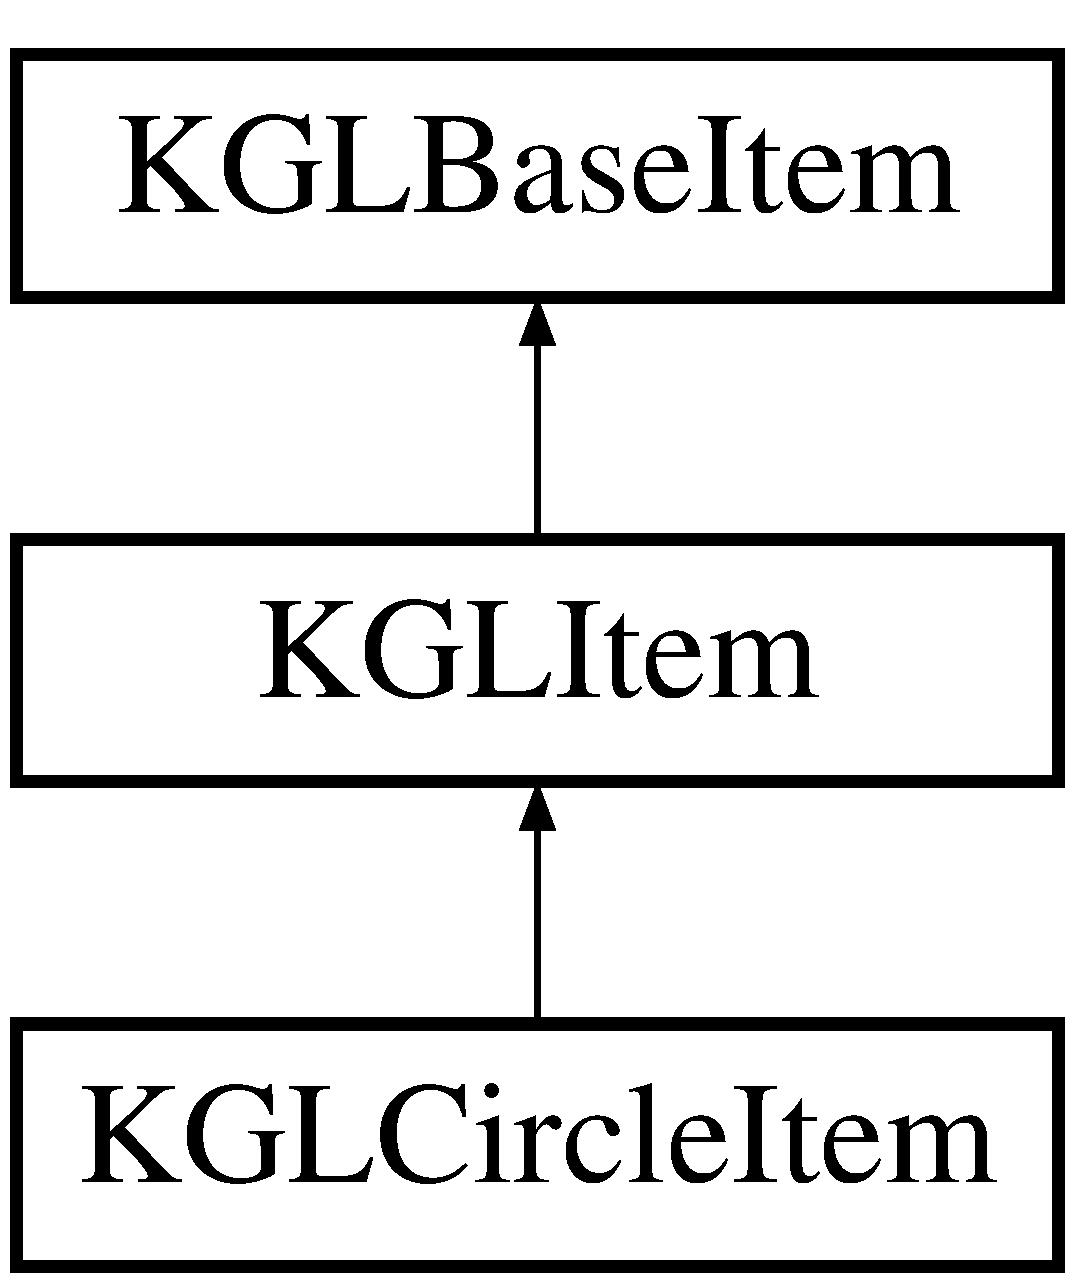
\includegraphics[height=3cm]{class_k_g_l_circle_item}
\end{center}
\end{figure}
\subsection*{Public Member Functions}
\begin{CompactItemize}
\item 
\hyperlink{class_k_g_l_circle_item_20c2a9aa6bfc35947dba70b84c0746b5}{KGLCircleItem} (float radius, unsigned int nbPoints=10, \hyperlink{class_k_g_l_engine}{KGLEngine} $\ast$parent=0)
\item 
void \hyperlink{class_k_g_l_circle_item_0a0419138f452f5d0e65fb28c77bda96}{setCircle} (float radius, unsigned int nbPoints)
\end{CompactItemize}


\subsection{Detailed Description}
This is a \hyperlink{class_k_g_l_item}{KGLItem} subclass for creating circles 

\subsection{Constructor \& Destructor Documentation}
\hypertarget{class_k_g_l_circle_item_20c2a9aa6bfc35947dba70b84c0746b5}{
\index{KGLCircleItem@{KGLCircleItem}!KGLCircleItem@{KGLCircleItem}}
\index{KGLCircleItem@{KGLCircleItem}!KGLCircleItem@{KGLCircleItem}}
\subsubsection[{KGLCircleItem}]{\setlength{\rightskip}{0pt plus 5cm}KGLCircleItem::KGLCircleItem (float {\em radius}, \/  unsigned int {\em nbPoints} = {\tt 10}, \/  {\bf KGLEngine} $\ast$ {\em parent} = {\tt 0})\hspace{0.3cm}{\tt  \mbox{[}explicit\mbox{]}}}}
\label{class_k_g_l_circle_item_20c2a9aa6bfc35947dba70b84c0746b5}




\subsection{Member Function Documentation}
\hypertarget{class_k_g_l_circle_item_0a0419138f452f5d0e65fb28c77bda96}{
\index{KGLCircleItem@{KGLCircleItem}!setCircle@{setCircle}}
\index{setCircle@{setCircle}!KGLCircleItem@{KGLCircleItem}}
\subsubsection[{setCircle}]{\setlength{\rightskip}{0pt plus 5cm}void KGLCircleItem::setCircle (float {\em radius}, \/  unsigned int {\em nbPoints})}}
\label{class_k_g_l_circle_item_0a0419138f452f5d0e65fb28c77bda96}




The documentation for this class was generated from the following files:\begin{CompactItemize}
\item 
/home/sacha/programmation/gluon/kgl/\hyperlink{kglcircleitem_8h}{kglcircleitem.h}\item 
/home/sacha/programmation/gluon/kgl/\hyperlink{kglcircleitem_8cpp}{kglcircleitem.cpp}\end{CompactItemize}

\hypertarget{class_k_g_l_contact_listener}{
\section{KGLContactListener Class Reference}
\label{class_k_g_l_contact_listener}\index{KGLContactListener@{KGLContactListener}}
}
{\tt \#include $<$kglphysicsengine.h$>$}

\subsection*{Public Member Functions}
\begin{CompactItemize}
\item 
void \hyperlink{class_k_g_l_contact_listener_c1e0677225b0ee3140963d78bc99ae8f}{Add} (const b2ContactPoint $\ast$point)
\end{CompactItemize}


\subsection{Member Function Documentation}
\hypertarget{class_k_g_l_contact_listener_c1e0677225b0ee3140963d78bc99ae8f}{
\index{KGLContactListener@{KGLContactListener}!Add@{Add}}
\index{Add@{Add}!KGLContactListener@{KGLContactListener}}
\subsubsection[{Add}]{\setlength{\rightskip}{0pt plus 5cm}void KGLContactListener::Add (const b2ContactPoint $\ast$ {\em point})}}
\label{class_k_g_l_contact_listener_c1e0677225b0ee3140963d78bc99ae8f}




The documentation for this class was generated from the following files:\begin{CompactItemize}
\item 
/home/sacha/programmation/gluon/kgl/\hyperlink{kglphysicsengine_8h}{kglphysicsengine.h}\item 
/home/sacha/programmation/gluon/kgl/\hyperlink{kglphysicsengine_8cpp}{kglphysicsengine.cpp}\end{CompactItemize}

\hypertarget{class_k_g_l_container_item}{
\section{KGLContainerItem Class Reference}
\label{class_k_g_l_container_item}\index{KGLContainerItem@{KGLContainerItem}}
}
{\tt \#include $<$kglcontaineritem.h$>$}

Inheritance diagram for KGLContainerItem::\begin{figure}[H]
\begin{center}
\leavevmode
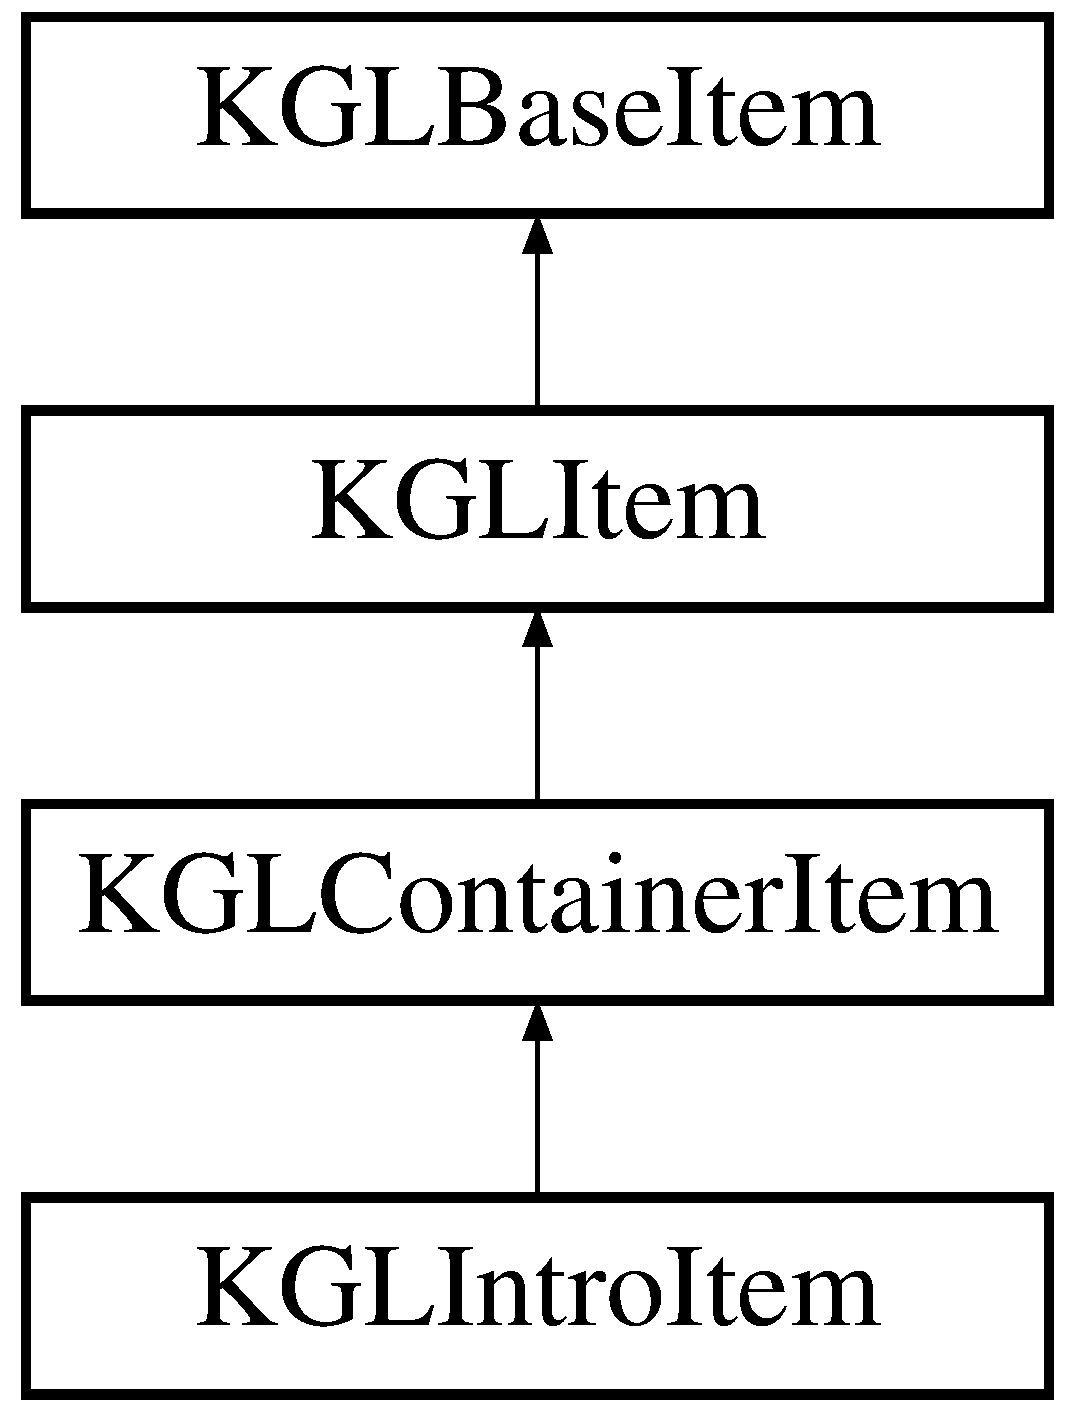
\includegraphics[height=4cm]{class_k_g_l_container_item}
\end{center}
\end{figure}
\subsection*{Public Member Functions}
\begin{CompactItemize}
\item 
\hyperlink{class_k_g_l_container_item_528a22298dba0b7d924d815021974f21}{KGLContainerItem} (QObject $\ast$parent=0)
\item 
virtual \hyperlink{class_k_g_l_container_item_3423869f556bf2b5949fe49c91e6d2f0}{$\sim$KGLContainerItem} ()
\item 
virtual void \hyperlink{class_k_g_l_container_item_a785dc67935db5f335c74e4a7fb685b9}{draw} ()
\item 
void \hyperlink{class_k_g_l_container_item_1fb6362381fbdd8270b02d66d5b02181}{addChild} (\hyperlink{class_k_g_l_item}{KGLItem} $\ast$item)
\item 
void \hyperlink{class_k_g_l_container_item_a95f051ed6ff3c4603023a3edf48d1e9}{eraseChild} (\hyperlink{class_k_g_l_item}{KGLItem} $\ast$item)
\item 
const \hyperlink{class_k_g_l_item_list}{KGLItemList} \hyperlink{class_k_g_l_container_item_3ade56aba64c289d67dfb1762c161182}{childItems} () const 
\end{CompactItemize}
\subsection*{Protected Attributes}
\begin{CompactItemize}
\item 
\hyperlink{class_k_g_l_item_list}{KGLItemList} \hyperlink{class_k_g_l_container_item_1bfbe0d002c10f18687b3bd59b97f6d3}{m\_\-children}
\end{CompactItemize}


\subsection{Constructor \& Destructor Documentation}
\hypertarget{class_k_g_l_container_item_528a22298dba0b7d924d815021974f21}{
\index{KGLContainerItem@{KGLContainerItem}!KGLContainerItem@{KGLContainerItem}}
\index{KGLContainerItem@{KGLContainerItem}!KGLContainerItem@{KGLContainerItem}}
\subsubsection[{KGLContainerItem}]{\setlength{\rightskip}{0pt plus 5cm}KGLContainerItem::KGLContainerItem (QObject $\ast$ {\em parent} = {\tt 0})}}
\label{class_k_g_l_container_item_528a22298dba0b7d924d815021974f21}


\hypertarget{class_k_g_l_container_item_3423869f556bf2b5949fe49c91e6d2f0}{
\index{KGLContainerItem@{KGLContainerItem}!$\sim$KGLContainerItem@{$\sim$KGLContainerItem}}
\index{$\sim$KGLContainerItem@{$\sim$KGLContainerItem}!KGLContainerItem@{KGLContainerItem}}
\subsubsection[{$\sim$KGLContainerItem}]{\setlength{\rightskip}{0pt plus 5cm}KGLContainerItem::$\sim$KGLContainerItem ()\hspace{0.3cm}{\tt  \mbox{[}virtual\mbox{]}}}}
\label{class_k_g_l_container_item_3423869f556bf2b5949fe49c91e6d2f0}




\subsection{Member Function Documentation}
\hypertarget{class_k_g_l_container_item_1fb6362381fbdd8270b02d66d5b02181}{
\index{KGLContainerItem@{KGLContainerItem}!addChild@{addChild}}
\index{addChild@{addChild}!KGLContainerItem@{KGLContainerItem}}
\subsubsection[{addChild}]{\setlength{\rightskip}{0pt plus 5cm}void KGLContainerItem::addChild ({\bf KGLItem} $\ast$ {\em item})}}
\label{class_k_g_l_container_item_1fb6362381fbdd8270b02d66d5b02181}


\hypertarget{class_k_g_l_container_item_3ade56aba64c289d67dfb1762c161182}{
\index{KGLContainerItem@{KGLContainerItem}!childItems@{childItems}}
\index{childItems@{childItems}!KGLContainerItem@{KGLContainerItem}}
\subsubsection[{childItems}]{\setlength{\rightskip}{0pt plus 5cm}const {\bf KGLItemList} KGLContainerItem::childItems () const\hspace{0.3cm}{\tt  \mbox{[}inline\mbox{]}}}}
\label{class_k_g_l_container_item_3ade56aba64c289d67dfb1762c161182}


\hypertarget{class_k_g_l_container_item_a785dc67935db5f335c74e4a7fb685b9}{
\index{KGLContainerItem@{KGLContainerItem}!draw@{draw}}
\index{draw@{draw}!KGLContainerItem@{KGLContainerItem}}
\subsubsection[{draw}]{\setlength{\rightskip}{0pt plus 5cm}void KGLContainerItem::draw ()\hspace{0.3cm}{\tt  \mbox{[}virtual\mbox{]}}}}
\label{class_k_g_l_container_item_a785dc67935db5f335c74e4a7fb685b9}




Reimplemented from \hyperlink{class_k_g_l_item_4e4766cf0362fa050bffdf5f45d6d13f}{KGLItem}.\hypertarget{class_k_g_l_container_item_a95f051ed6ff3c4603023a3edf48d1e9}{
\index{KGLContainerItem@{KGLContainerItem}!eraseChild@{eraseChild}}
\index{eraseChild@{eraseChild}!KGLContainerItem@{KGLContainerItem}}
\subsubsection[{eraseChild}]{\setlength{\rightskip}{0pt plus 5cm}void KGLContainerItem::eraseChild ({\bf KGLItem} $\ast$ {\em item})\hspace{0.3cm}{\tt  \mbox{[}inline\mbox{]}}}}
\label{class_k_g_l_container_item_a95f051ed6ff3c4603023a3edf48d1e9}




\subsection{Member Data Documentation}
\hypertarget{class_k_g_l_container_item_1bfbe0d002c10f18687b3bd59b97f6d3}{
\index{KGLContainerItem@{KGLContainerItem}!m\_\-children@{m\_\-children}}
\index{m\_\-children@{m\_\-children}!KGLContainerItem@{KGLContainerItem}}
\subsubsection[{m\_\-children}]{\setlength{\rightskip}{0pt plus 5cm}{\bf KGLItemList} {\bf KGLContainerItem::m\_\-children}\hspace{0.3cm}{\tt  \mbox{[}protected\mbox{]}}}}
\label{class_k_g_l_container_item_1bfbe0d002c10f18687b3bd59b97f6d3}




The documentation for this class was generated from the following files:\begin{CompactItemize}
\item 
/home/sacha/programmation/gluon/kgl/\hyperlink{kglcontaineritem_8h}{kglcontaineritem.h}\item 
/home/sacha/programmation/gluon/kgl/\hyperlink{kglcontaineritem_8cpp}{kglcontaineritem.cpp}\end{CompactItemize}

\hypertarget{class_k_g_l_engine}{
\section{KGLEngine Class Reference}
\label{class_k_g_l_engine}\index{KGLEngine@{KGLEngine}}
}
{\tt \#include $<$kglengine.h$>$}

Inheritance diagram for KGLEngine::\begin{figure}[H]
\begin{center}
\leavevmode
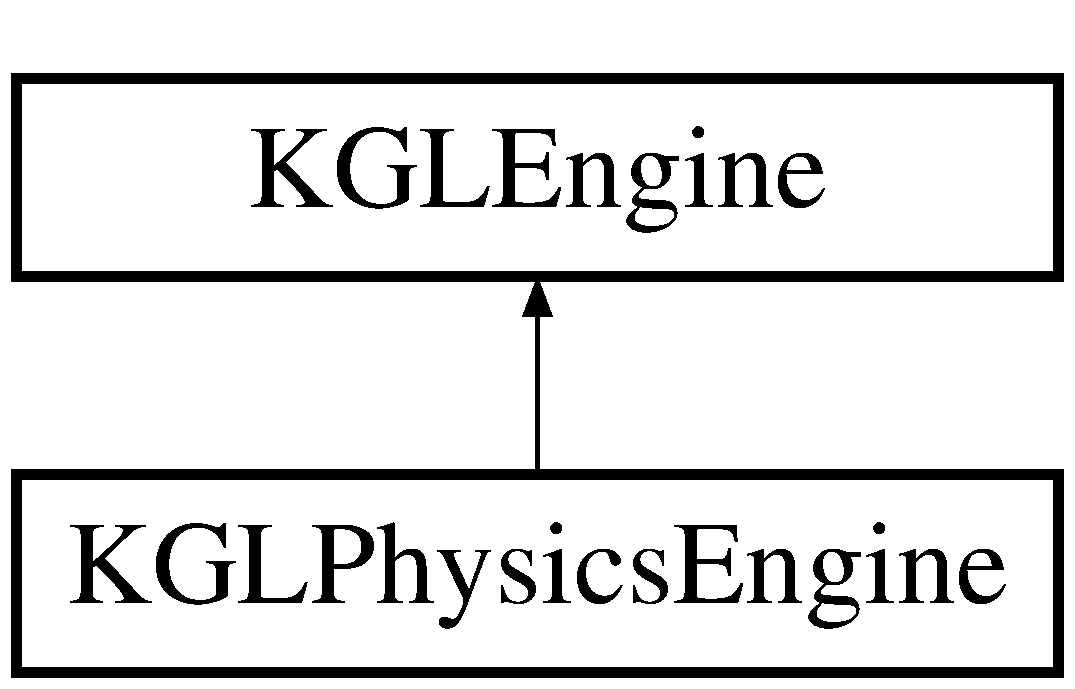
\includegraphics[height=2cm]{class_k_g_l_engine}
\end{center}
\end{figure}
\subsection*{Public Member Functions}
\begin{CompactItemize}
\item 
\hyperlink{class_k_g_l_engine_6f462f4b94e90736eebe4bc97c9639ea}{KGLEngine} (QObject $\ast$parent=0)
\item 
virtual void \hyperlink{class_k_g_l_engine_787e1d8dfb58a6d6973a1f62c83b3263}{mainLoop} (float fps=60)
\item 
void \hyperlink{class_k_g_l_engine_4aa9d5809d76cc44994a1cdb9df6f3ec}{addItem} (\hyperlink{class_k_g_l_item}{KGLItem} $\ast$item)
\item 
void \hyperlink{class_k_g_l_engine_0b25939d43f254ed6650bf9cded68f60}{addItems} (const \hyperlink{class_k_g_l_item_list}{KGLItemList} $\ast$items)
\item 
bool \hyperlink{class_k_g_l_engine_533f3324f67dcda39192365e2eab40c3}{removeItem} (\hyperlink{class_k_g_l_item}{KGLItem} $\ast$item)
\item 
bool \hyperlink{class_k_g_l_engine_11d424c95a9adf619c36627a6d509072}{removeItems} (const \hyperlink{class_k_g_l_item_list}{KGLItemList} $\ast$item)
\item 
virtual bool \hyperlink{class_k_g_l_engine_66aa5b9783823cf7db5edcc50981999a}{eraseItem} (\hyperlink{class_k_g_l_item}{KGLItem} $\ast$item)
\item 
bool \hyperlink{class_k_g_l_engine_b7f3be194234b978df3f59769f565588}{eraseItems} (const \hyperlink{class_k_g_l_item_list}{KGLItemList} $\ast$item)
\item 
\hyperlink{class_k_g_l_item}{KGLItem} $\ast$ \hyperlink{class_k_g_l_engine_ac35be1039af0dbc2dc208774f085795}{itemAt} (int id, unsigned int layer=0)
\item 
int \hyperlink{class_k_g_l_engine_1cc02d12efbc07e9a40d420f081ba588}{itemsCount} () const 
\item 
\hyperlink{class_k_g_l_box_item}{KGLBoxItem} $\ast$ \hyperlink{class_k_g_l_engine_428426702fca3958cc3ee41149312d68}{addBox} (float w, float h)
\item 
\hyperlink{kglengine_8h_b80cbcec260e71c3207c42d7eba43da1}{IndexGroupMap} \hyperlink{class_k_g_l_engine_4b105206ea488eea87e835339d5473b5}{items} ()
\end{CompactItemize}


\subsection{Constructor \& Destructor Documentation}
\hypertarget{class_k_g_l_engine_6f462f4b94e90736eebe4bc97c9639ea}{
\index{KGLEngine@{KGLEngine}!KGLEngine@{KGLEngine}}
\index{KGLEngine@{KGLEngine}!KGLEngine@{KGLEngine}}
\subsubsection[{KGLEngine}]{\setlength{\rightskip}{0pt plus 5cm}KGLEngine::KGLEngine (QObject $\ast$ {\em parent} = {\tt 0})}}
\label{class_k_g_l_engine_6f462f4b94e90736eebe4bc97c9639ea}




\subsection{Member Function Documentation}
\hypertarget{class_k_g_l_engine_428426702fca3958cc3ee41149312d68}{
\index{KGLEngine@{KGLEngine}!addBox@{addBox}}
\index{addBox@{addBox}!KGLEngine@{KGLEngine}}
\subsubsection[{addBox}]{\setlength{\rightskip}{0pt plus 5cm}{\bf KGLBoxItem}$\ast$ KGLEngine::addBox (float {\em w}, \/  float {\em h})\hspace{0.3cm}{\tt  \mbox{[}inline\mbox{]}}}}
\label{class_k_g_l_engine_428426702fca3958cc3ee41149312d68}


\hypertarget{class_k_g_l_engine_4aa9d5809d76cc44994a1cdb9df6f3ec}{
\index{KGLEngine@{KGLEngine}!addItem@{addItem}}
\index{addItem@{addItem}!KGLEngine@{KGLEngine}}
\subsubsection[{addItem}]{\setlength{\rightskip}{0pt plus 5cm}void KGLEngine::addItem ({\bf KGLItem} $\ast$ {\em item})}}
\label{class_k_g_l_engine_4aa9d5809d76cc44994a1cdb9df6f3ec}




Reimplemented in \hyperlink{class_k_g_l_physics_engine_eefe31c558a83c43d1840987cdea1898}{KGLPhysicsEngine}.\hypertarget{class_k_g_l_engine_0b25939d43f254ed6650bf9cded68f60}{
\index{KGLEngine@{KGLEngine}!addItems@{addItems}}
\index{addItems@{addItems}!KGLEngine@{KGLEngine}}
\subsubsection[{addItems}]{\setlength{\rightskip}{0pt plus 5cm}void KGLEngine::addItems (const {\bf KGLItemList} $\ast$ {\em items})}}
\label{class_k_g_l_engine_0b25939d43f254ed6650bf9cded68f60}


\hypertarget{class_k_g_l_engine_66aa5b9783823cf7db5edcc50981999a}{
\index{KGLEngine@{KGLEngine}!eraseItem@{eraseItem}}
\index{eraseItem@{eraseItem}!KGLEngine@{KGLEngine}}
\subsubsection[{eraseItem}]{\setlength{\rightskip}{0pt plus 5cm}bool KGLEngine::eraseItem ({\bf KGLItem} $\ast$ {\em item})\hspace{0.3cm}{\tt  \mbox{[}virtual\mbox{]}}}}
\label{class_k_g_l_engine_66aa5b9783823cf7db5edcc50981999a}


\hypertarget{class_k_g_l_engine_b7f3be194234b978df3f59769f565588}{
\index{KGLEngine@{KGLEngine}!eraseItems@{eraseItems}}
\index{eraseItems@{eraseItems}!KGLEngine@{KGLEngine}}
\subsubsection[{eraseItems}]{\setlength{\rightskip}{0pt plus 5cm}bool KGLEngine::eraseItems (const {\bf KGLItemList} $\ast$ {\em item})}}
\label{class_k_g_l_engine_b7f3be194234b978df3f59769f565588}


\hypertarget{class_k_g_l_engine_ac35be1039af0dbc2dc208774f085795}{
\index{KGLEngine@{KGLEngine}!itemAt@{itemAt}}
\index{itemAt@{itemAt}!KGLEngine@{KGLEngine}}
\subsubsection[{itemAt}]{\setlength{\rightskip}{0pt plus 5cm}{\bf KGLItem} $\ast$ KGLEngine::itemAt (int {\em id}, \/  unsigned int {\em layer} = {\tt 0})}}
\label{class_k_g_l_engine_ac35be1039af0dbc2dc208774f085795}


\hypertarget{class_k_g_l_engine_4b105206ea488eea87e835339d5473b5}{
\index{KGLEngine@{KGLEngine}!items@{items}}
\index{items@{items}!KGLEngine@{KGLEngine}}
\subsubsection[{items}]{\setlength{\rightskip}{0pt plus 5cm}{\bf IndexGroupMap} KGLEngine::items ()\hspace{0.3cm}{\tt  \mbox{[}inline\mbox{]}}}}
\label{class_k_g_l_engine_4b105206ea488eea87e835339d5473b5}


\hypertarget{class_k_g_l_engine_1cc02d12efbc07e9a40d420f081ba588}{
\index{KGLEngine@{KGLEngine}!itemsCount@{itemsCount}}
\index{itemsCount@{itemsCount}!KGLEngine@{KGLEngine}}
\subsubsection[{itemsCount}]{\setlength{\rightskip}{0pt plus 5cm}int KGLEngine::itemsCount () const}}
\label{class_k_g_l_engine_1cc02d12efbc07e9a40d420f081ba588}


\hypertarget{class_k_g_l_engine_787e1d8dfb58a6d6973a1f62c83b3263}{
\index{KGLEngine@{KGLEngine}!mainLoop@{mainLoop}}
\index{mainLoop@{mainLoop}!KGLEngine@{KGLEngine}}
\subsubsection[{mainLoop}]{\setlength{\rightskip}{0pt plus 5cm}void KGLEngine::mainLoop (float {\em fps} = {\tt 60})\hspace{0.3cm}{\tt  \mbox{[}virtual\mbox{]}}}}
\label{class_k_g_l_engine_787e1d8dfb58a6d6973a1f62c83b3263}




Reimplemented in \hyperlink{class_k_g_l_physics_engine_b72358d3b45888792d7c4e91715d29b4}{KGLPhysicsEngine}.\hypertarget{class_k_g_l_engine_533f3324f67dcda39192365e2eab40c3}{
\index{KGLEngine@{KGLEngine}!removeItem@{removeItem}}
\index{removeItem@{removeItem}!KGLEngine@{KGLEngine}}
\subsubsection[{removeItem}]{\setlength{\rightskip}{0pt plus 5cm}bool KGLEngine::removeItem ({\bf KGLItem} $\ast$ {\em item})}}
\label{class_k_g_l_engine_533f3324f67dcda39192365e2eab40c3}




Reimplemented in \hyperlink{class_k_g_l_physics_engine_c5e88c0ab7ec1923038fdcb36ffdb192}{KGLPhysicsEngine}.\hypertarget{class_k_g_l_engine_11d424c95a9adf619c36627a6d509072}{
\index{KGLEngine@{KGLEngine}!removeItems@{removeItems}}
\index{removeItems@{removeItems}!KGLEngine@{KGLEngine}}
\subsubsection[{removeItems}]{\setlength{\rightskip}{0pt plus 5cm}bool KGLEngine::removeItems (const {\bf KGLItemList} $\ast$ {\em item})}}
\label{class_k_g_l_engine_11d424c95a9adf619c36627a6d509072}




The documentation for this class was generated from the following files:\begin{CompactItemize}
\item 
/home/sacha/programmation/gluon/kgl/\hyperlink{kglengine_8h}{kglengine.h}\item 
/home/sacha/programmation/gluon/kgl/\hyperlink{kglengine_8cpp}{kglengine.cpp}\end{CompactItemize}

\hypertarget{class_k_g_l_fragment_shader}{
\section{KGLFragmentShader Class Reference}
\label{class_k_g_l_fragment_shader}\index{KGLFragmentShader@{KGLFragmentShader}}
}
{\tt \#include $<$kglshader.h$>$}

Inheritance diagram for KGLFragmentShader::\begin{figure}[H]
\begin{center}
\leavevmode
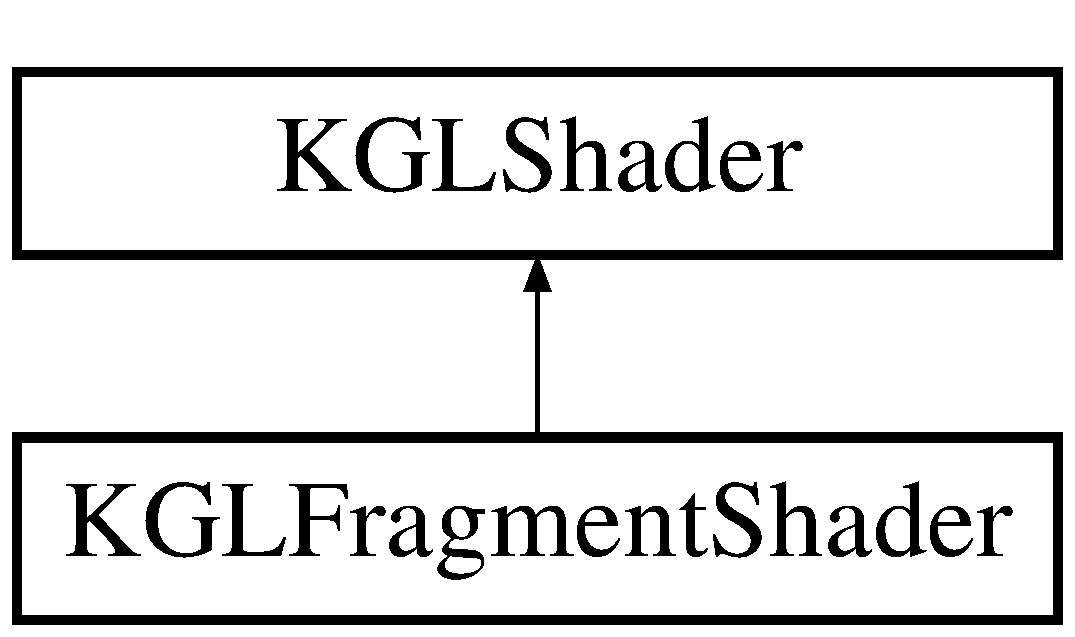
\includegraphics[height=2cm]{class_k_g_l_fragment_shader}
\end{center}
\end{figure}
\subsection*{Public Member Functions}
\begin{CompactItemize}
\item 
\hyperlink{class_k_g_l_fragment_shader_6cb6f1dc7de6a8ce0930a3cb14116444}{KGLFragmentShader} ()
\item 
\hyperlink{class_k_g_l_fragment_shader_63789f9dfc6cfe19d7423ff6540ca53d}{KGLFragmentShader} (const QString \&filename)
\end{CompactItemize}


\subsection{Detailed Description}
Fragment shader subclass, so you needn't pass the type=GL\_\-FRAGMENT\_\-SHADER parameter to Shader constructor yourself. 

\subsection{Constructor \& Destructor Documentation}
\hypertarget{class_k_g_l_fragment_shader_6cb6f1dc7de6a8ce0930a3cb14116444}{
\index{KGLFragmentShader@{KGLFragmentShader}!KGLFragmentShader@{KGLFragmentShader}}
\index{KGLFragmentShader@{KGLFragmentShader}!KGLFragmentShader@{KGLFragmentShader}}
\subsubsection[{KGLFragmentShader}]{\setlength{\rightskip}{0pt plus 5cm}KGLFragmentShader::KGLFragmentShader ()}}
\label{class_k_g_l_fragment_shader_6cb6f1dc7de6a8ce0930a3cb14116444}


\hypertarget{class_k_g_l_fragment_shader_63789f9dfc6cfe19d7423ff6540ca53d}{
\index{KGLFragmentShader@{KGLFragmentShader}!KGLFragmentShader@{KGLFragmentShader}}
\index{KGLFragmentShader@{KGLFragmentShader}!KGLFragmentShader@{KGLFragmentShader}}
\subsubsection[{KGLFragmentShader}]{\setlength{\rightskip}{0pt plus 5cm}KGLFragmentShader::KGLFragmentShader (const QString \& {\em filename})}}
\label{class_k_g_l_fragment_shader_63789f9dfc6cfe19d7423ff6540ca53d}




The documentation for this class was generated from the following files:\begin{CompactItemize}
\item 
/home/sacha/programmation/gluon/kgl/\hyperlink{kglshader_8h}{kglshader.h}\item 
/home/sacha/programmation/gluon/kgl/\hyperlink{kglshader_8cpp}{kglshader.cpp}\end{CompactItemize}

\hypertarget{class_k_g_l_fx}{
\section{KGLFx Class Reference}
\label{class_k_g_l_fx}\index{KGLFx@{KGLFx}}
}
{\tt \#include $<$kglfx.h$>$}

Inheritance diagram for KGLFx::\begin{figure}[H]
\begin{center}
\leavevmode
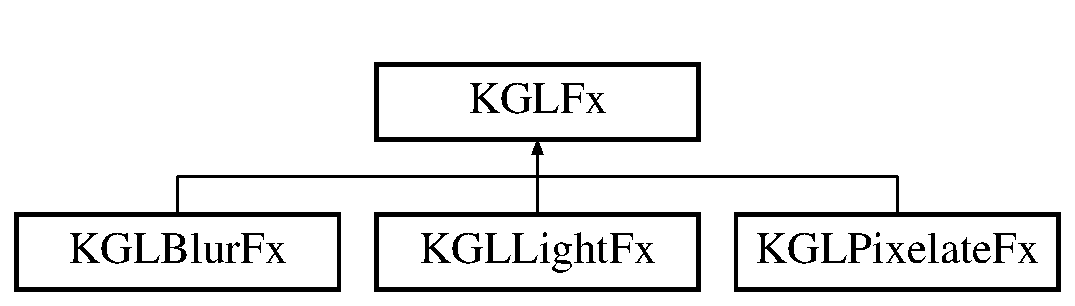
\includegraphics[height=2cm]{class_k_g_l_fx}
\end{center}
\end{figure}
\subsection*{Public Member Functions}
\begin{CompactItemize}
\item 
\hyperlink{class_k_g_l_fx_dd30f0c4b9ed54ee0be6d9cfd72890e8}{KGLFx} ()
\item 
void \hyperlink{class_k_g_l_fx_b96fa94be7e76720b806a098ffb8ee34}{bind} ()
\item 
void \hyperlink{class_k_g_l_fx_b3eaa1c6e1c562b43374bc4d1b670967}{unbind} ()
\item 
bool \hyperlink{class_k_g_l_fx_768cebc0d09e441e398ef4a5ac06f28a}{enable} ()
\item 
\hyperlink{class_k_g_l_program}{KGLProgram} $\ast$ \hyperlink{class_k_g_l_fx_c02c704f61750f6eb5b49f48d0a74820}{program} ()
\item 
void \hyperlink{class_k_g_l_fx_ce266e6c653796d142396ce056ec1b96}{setArg} (const char $\ast$name, int value)
\item 
void \hyperlink{class_k_g_l_fx_4406ef8524d0e53f64d30f7b6e229bc3}{setArg} (const char $\ast$name, float value)
\end{CompactItemize}


\subsection{Constructor \& Destructor Documentation}
\hypertarget{class_k_g_l_fx_dd30f0c4b9ed54ee0be6d9cfd72890e8}{
\index{KGLFx@{KGLFx}!KGLFx@{KGLFx}}
\index{KGLFx@{KGLFx}!KGLFx@{KGLFx}}
\subsubsection[{KGLFx}]{\setlength{\rightskip}{0pt plus 5cm}KGLFx::KGLFx ()}}
\label{class_k_g_l_fx_dd30f0c4b9ed54ee0be6d9cfd72890e8}




\subsection{Member Function Documentation}
\hypertarget{class_k_g_l_fx_b96fa94be7e76720b806a098ffb8ee34}{
\index{KGLFx@{KGLFx}!bind@{bind}}
\index{bind@{bind}!KGLFx@{KGLFx}}
\subsubsection[{bind}]{\setlength{\rightskip}{0pt plus 5cm}void KGLFx::bind ()\hspace{0.3cm}{\tt  \mbox{[}inline\mbox{]}}}}
\label{class_k_g_l_fx_b96fa94be7e76720b806a098ffb8ee34}


\hypertarget{class_k_g_l_fx_768cebc0d09e441e398ef4a5ac06f28a}{
\index{KGLFx@{KGLFx}!enable@{enable}}
\index{enable@{enable}!KGLFx@{KGLFx}}
\subsubsection[{enable}]{\setlength{\rightskip}{0pt plus 5cm}bool KGLFx::enable ()\hspace{0.3cm}{\tt  \mbox{[}inline\mbox{]}}}}
\label{class_k_g_l_fx_768cebc0d09e441e398ef4a5ac06f28a}


\hypertarget{class_k_g_l_fx_c02c704f61750f6eb5b49f48d0a74820}{
\index{KGLFx@{KGLFx}!program@{program}}
\index{program@{program}!KGLFx@{KGLFx}}
\subsubsection[{program}]{\setlength{\rightskip}{0pt plus 5cm}{\bf KGLProgram}$\ast$ KGLFx::program ()\hspace{0.3cm}{\tt  \mbox{[}inline\mbox{]}}}}
\label{class_k_g_l_fx_c02c704f61750f6eb5b49f48d0a74820}


\hypertarget{class_k_g_l_fx_4406ef8524d0e53f64d30f7b6e229bc3}{
\index{KGLFx@{KGLFx}!setArg@{setArg}}
\index{setArg@{setArg}!KGLFx@{KGLFx}}
\subsubsection[{setArg}]{\setlength{\rightskip}{0pt plus 5cm}void KGLFx::setArg (const char $\ast$ {\em name}, \/  float {\em value})\hspace{0.3cm}{\tt  \mbox{[}inline\mbox{]}}}}
\label{class_k_g_l_fx_4406ef8524d0e53f64d30f7b6e229bc3}


\hypertarget{class_k_g_l_fx_ce266e6c653796d142396ce056ec1b96}{
\index{KGLFx@{KGLFx}!setArg@{setArg}}
\index{setArg@{setArg}!KGLFx@{KGLFx}}
\subsubsection[{setArg}]{\setlength{\rightskip}{0pt plus 5cm}void KGLFx::setArg (const char $\ast$ {\em name}, \/  int {\em value})\hspace{0.3cm}{\tt  \mbox{[}inline\mbox{]}}}}
\label{class_k_g_l_fx_ce266e6c653796d142396ce056ec1b96}


\hypertarget{class_k_g_l_fx_b3eaa1c6e1c562b43374bc4d1b670967}{
\index{KGLFx@{KGLFx}!unbind@{unbind}}
\index{unbind@{unbind}!KGLFx@{KGLFx}}
\subsubsection[{unbind}]{\setlength{\rightskip}{0pt plus 5cm}void KGLFx::unbind ()\hspace{0.3cm}{\tt  \mbox{[}inline\mbox{]}}}}
\label{class_k_g_l_fx_b3eaa1c6e1c562b43374bc4d1b670967}




The documentation for this class was generated from the following files:\begin{CompactItemize}
\item 
/home/sacha/programmation/gluon/kgl/\hyperlink{kglfx_8h}{kglfx.h}\item 
/home/sacha/programmation/gluon/kgl/\hyperlink{kglfx_8cpp}{kglfx.cpp}\end{CompactItemize}

\hypertarget{class_k_g_l_grid_item}{
\section{KGLGridItem Class Reference}
\label{class_k_g_l_grid_item}\index{KGLGridItem@{KGLGridItem}}
}
{\tt \#include $<$kglgriditem.h$>$}

Inheritance diagram for KGLGridItem::\begin{figure}[H]
\begin{center}
\leavevmode
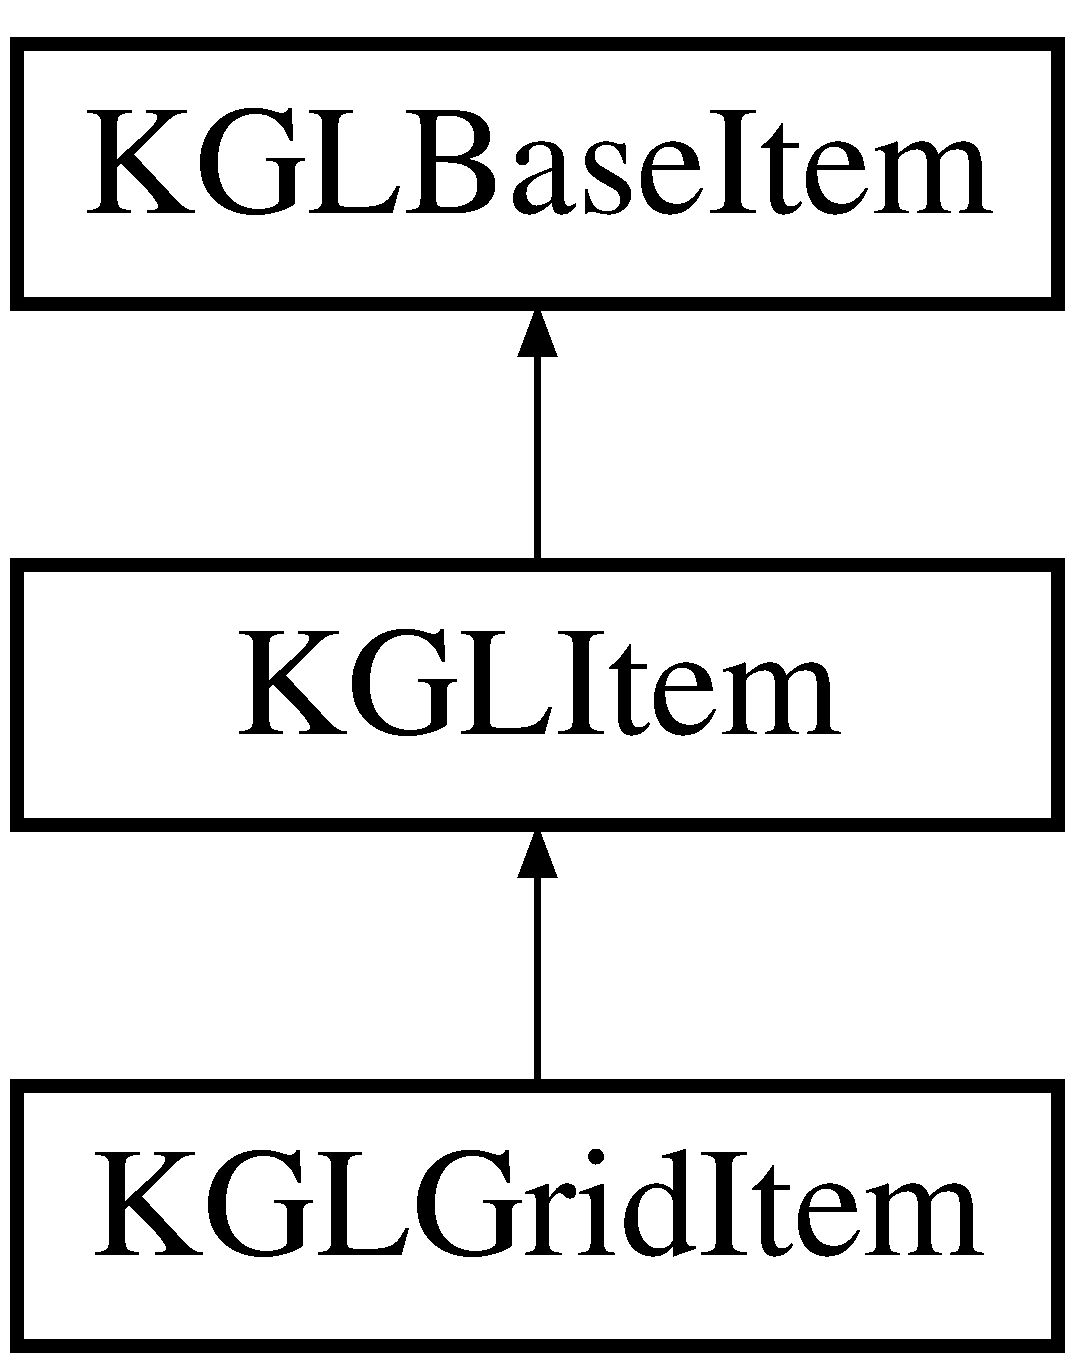
\includegraphics[height=3cm]{class_k_g_l_grid_item}
\end{center}
\end{figure}
\subsection*{Public Member Functions}
\begin{CompactItemize}
\item 
\hyperlink{class_k_g_l_grid_item_8016e40bc98d55adc2b08674d2fa117e}{KGLGridItem} (QSizeF size, float tile=1, \hyperlink{class_k_g_l_engine}{KGLEngine} $\ast$engine=0)
\item 
\hyperlink{class_k_g_l_grid_item_217588549e34d03495e0a883e3445c78}{KGLGridItem} (float width, float height, float tile=1, \hyperlink{class_k_g_l_engine}{KGLEngine} $\ast$engine=0)
\item 
void \hyperlink{class_k_g_l_grid_item_b86b8c2552de5956e79abb6b0ce81d73}{init} ()
\item 
void \hyperlink{class_k_g_l_grid_item_4e80ff451f8c95bc540751ed8f2b9a76}{createGrid} ()
\item 
const \hyperlink{class_k_g_l_point}{KGLPoint} $\ast$ \hyperlink{class_k_g_l_grid_item_8141076182d7926b8a303639783286af}{pointAt} (QPoint p)
\item 
const \hyperlink{class_k_g_l_point}{KGLPoint} $\ast$ \hyperlink{class_k_g_l_grid_item_dcacb054e43744cdadf266eb544d827c}{pointAt} (int x, int y)
\item 
void \hyperlink{class_k_g_l_grid_item_5f2a3cccf7cf2ad90bf40e822907c660}{setSize} (const QSizeF \&s)
\item 
void \hyperlink{class_k_g_l_grid_item_7ca4ae016b8d4af31cddeea0654584df}{setTile} (const float \&t)
\end{CompactItemize}


\subsection{Constructor \& Destructor Documentation}
\hypertarget{class_k_g_l_grid_item_8016e40bc98d55adc2b08674d2fa117e}{
\index{KGLGridItem@{KGLGridItem}!KGLGridItem@{KGLGridItem}}
\index{KGLGridItem@{KGLGridItem}!KGLGridItem@{KGLGridItem}}
\subsubsection[{KGLGridItem}]{\setlength{\rightskip}{0pt plus 5cm}KGLGridItem::KGLGridItem (QSizeF {\em size}, \/  float {\em tile} = {\tt 1}, \/  {\bf KGLEngine} $\ast$ {\em engine} = {\tt 0})}}
\label{class_k_g_l_grid_item_8016e40bc98d55adc2b08674d2fa117e}


\hypertarget{class_k_g_l_grid_item_217588549e34d03495e0a883e3445c78}{
\index{KGLGridItem@{KGLGridItem}!KGLGridItem@{KGLGridItem}}
\index{KGLGridItem@{KGLGridItem}!KGLGridItem@{KGLGridItem}}
\subsubsection[{KGLGridItem}]{\setlength{\rightskip}{0pt plus 5cm}KGLGridItem::KGLGridItem (float {\em width}, \/  float {\em height}, \/  float {\em tile} = {\tt 1}, \/  {\bf KGLEngine} $\ast$ {\em engine} = {\tt 0})}}
\label{class_k_g_l_grid_item_217588549e34d03495e0a883e3445c78}




\subsection{Member Function Documentation}
\hypertarget{class_k_g_l_grid_item_4e80ff451f8c95bc540751ed8f2b9a76}{
\index{KGLGridItem@{KGLGridItem}!createGrid@{createGrid}}
\index{createGrid@{createGrid}!KGLGridItem@{KGLGridItem}}
\subsubsection[{createGrid}]{\setlength{\rightskip}{0pt plus 5cm}void KGLGridItem::createGrid ()}}
\label{class_k_g_l_grid_item_4e80ff451f8c95bc540751ed8f2b9a76}


\hypertarget{class_k_g_l_grid_item_b86b8c2552de5956e79abb6b0ce81d73}{
\index{KGLGridItem@{KGLGridItem}!init@{init}}
\index{init@{init}!KGLGridItem@{KGLGridItem}}
\subsubsection[{init}]{\setlength{\rightskip}{0pt plus 5cm}void KGLGridItem::init ()}}
\label{class_k_g_l_grid_item_b86b8c2552de5956e79abb6b0ce81d73}




Reimplemented from \hyperlink{class_k_g_l_item_2227b986b72366e149815a5fa5838d52}{KGLItem}.\hypertarget{class_k_g_l_grid_item_dcacb054e43744cdadf266eb544d827c}{
\index{KGLGridItem@{KGLGridItem}!pointAt@{pointAt}}
\index{pointAt@{pointAt}!KGLGridItem@{KGLGridItem}}
\subsubsection[{pointAt}]{\setlength{\rightskip}{0pt plus 5cm}const {\bf KGLPoint}$\ast$ KGLGridItem::pointAt (int {\em x}, \/  int {\em y})\hspace{0.3cm}{\tt  \mbox{[}inline\mbox{]}}}}
\label{class_k_g_l_grid_item_dcacb054e43744cdadf266eb544d827c}


\hypertarget{class_k_g_l_grid_item_8141076182d7926b8a303639783286af}{
\index{KGLGridItem@{KGLGridItem}!pointAt@{pointAt}}
\index{pointAt@{pointAt}!KGLGridItem@{KGLGridItem}}
\subsubsection[{pointAt}]{\setlength{\rightskip}{0pt plus 5cm}const {\bf KGLPoint} $\ast$ KGLGridItem::pointAt (QPoint {\em p})}}
\label{class_k_g_l_grid_item_8141076182d7926b8a303639783286af}


\hypertarget{class_k_g_l_grid_item_5f2a3cccf7cf2ad90bf40e822907c660}{
\index{KGLGridItem@{KGLGridItem}!setSize@{setSize}}
\index{setSize@{setSize}!KGLGridItem@{KGLGridItem}}
\subsubsection[{setSize}]{\setlength{\rightskip}{0pt plus 5cm}void KGLGridItem::setSize (const QSizeF \& {\em s})\hspace{0.3cm}{\tt  \mbox{[}inline\mbox{]}}}}
\label{class_k_g_l_grid_item_5f2a3cccf7cf2ad90bf40e822907c660}


\hypertarget{class_k_g_l_grid_item_7ca4ae016b8d4af31cddeea0654584df}{
\index{KGLGridItem@{KGLGridItem}!setTile@{setTile}}
\index{setTile@{setTile}!KGLGridItem@{KGLGridItem}}
\subsubsection[{setTile}]{\setlength{\rightskip}{0pt plus 5cm}void KGLGridItem::setTile (const float \& {\em t})\hspace{0.3cm}{\tt  \mbox{[}inline\mbox{]}}}}
\label{class_k_g_l_grid_item_7ca4ae016b8d4af31cddeea0654584df}




The documentation for this class was generated from the following files:\begin{CompactItemize}
\item 
/home/sacha/programmation/gluon/kgl/\hyperlink{kglgriditem_8h}{kglgriditem.h}\item 
/home/sacha/programmation/gluon/kgl/\hyperlink{kglgriditem_8cpp}{kglgriditem.cpp}\end{CompactItemize}

\hypertarget{class_k_g_l_intro_item}{
\section{KGLIntroItem Class Reference}
\label{class_k_g_l_intro_item}\index{KGLIntroItem@{KGLIntroItem}}
}
{\tt \#include $<$kglintro.h$>$}

Inheritance diagram for KGLIntroItem::\begin{figure}[H]
\begin{center}
\leavevmode
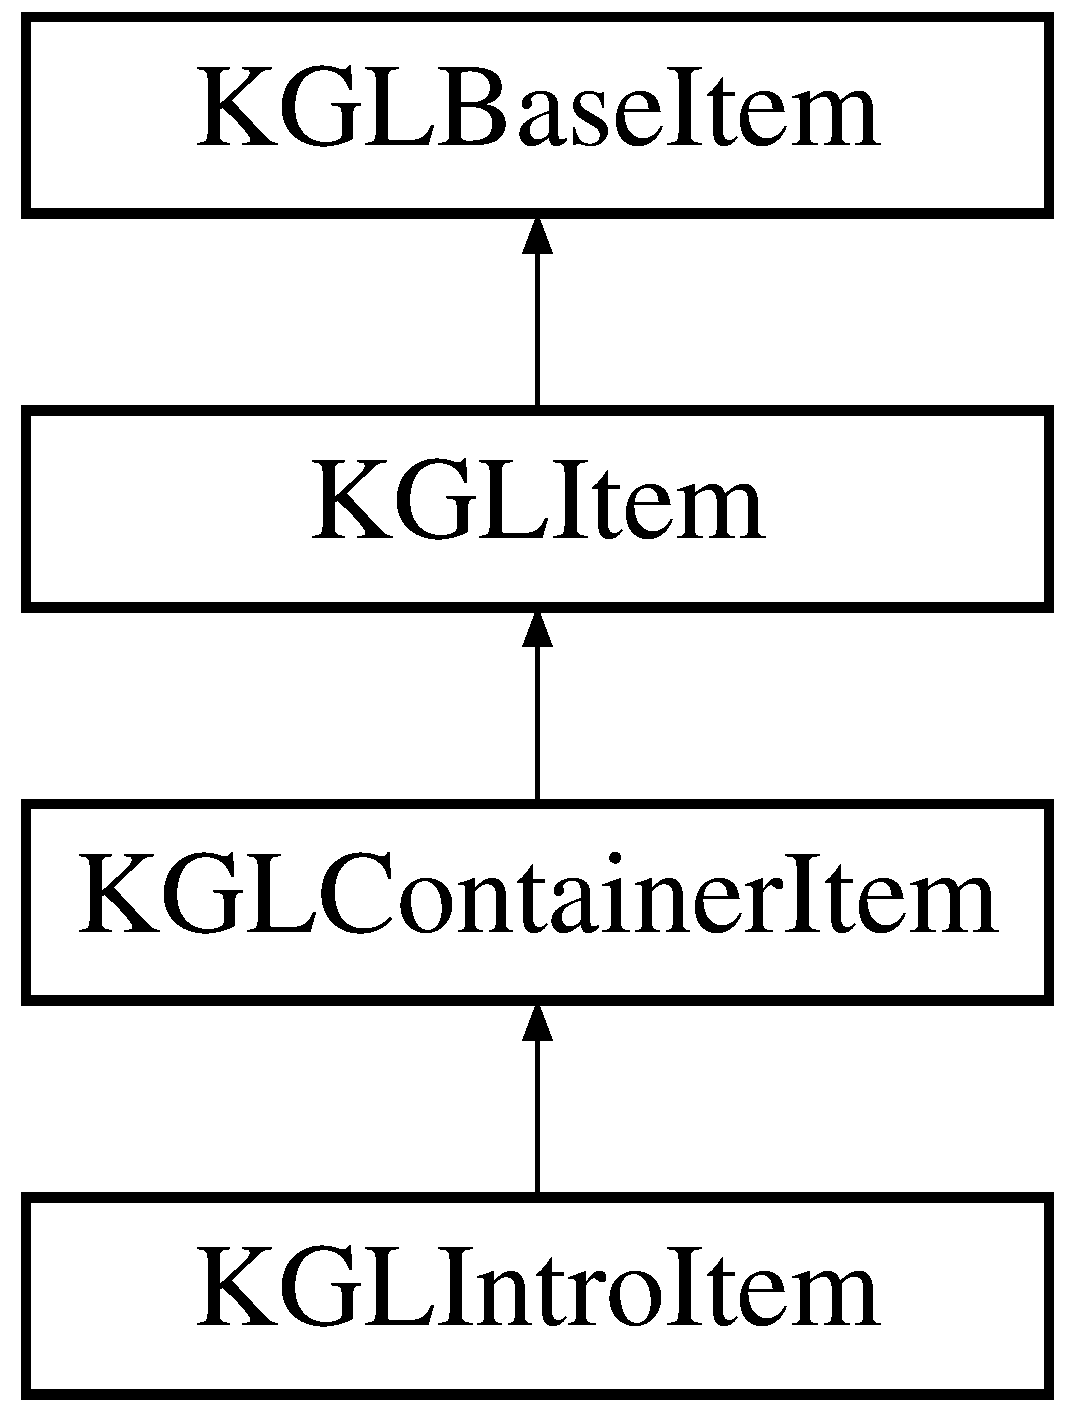
\includegraphics[height=4cm]{class_k_g_l_intro_item}
\end{center}
\end{figure}
\subsection*{Public Slots}
\begin{CompactItemize}
\item 
virtual void \hyperlink{class_k_g_l_intro_item_123f0b6f3fd34ed385a34b6485db7c2e}{anim} ()
\end{CompactItemize}
\subsection*{Public Member Functions}
\begin{CompactItemize}
\item 
\hyperlink{class_k_g_l_intro_item_66fdbf0f7893053ba01112f473b71f30}{KGLIntroItem} (QObject $\ast$parent=0)
\end{CompactItemize}


\subsection{Constructor \& Destructor Documentation}
\hypertarget{class_k_g_l_intro_item_66fdbf0f7893053ba01112f473b71f30}{
\index{KGLIntroItem@{KGLIntroItem}!KGLIntroItem@{KGLIntroItem}}
\index{KGLIntroItem@{KGLIntroItem}!KGLIntroItem@{KGLIntroItem}}
\subsubsection[{KGLIntroItem}]{\setlength{\rightskip}{0pt plus 5cm}KGLIntroItem::KGLIntroItem (QObject $\ast$ {\em parent} = {\tt 0})}}
\label{class_k_g_l_intro_item_66fdbf0f7893053ba01112f473b71f30}




\subsection{Member Function Documentation}
\hypertarget{class_k_g_l_intro_item_123f0b6f3fd34ed385a34b6485db7c2e}{
\index{KGLIntroItem@{KGLIntroItem}!anim@{anim}}
\index{anim@{anim}!KGLIntroItem@{KGLIntroItem}}
\subsubsection[{anim}]{\setlength{\rightskip}{0pt plus 5cm}void KGLIntroItem::anim ()\hspace{0.3cm}{\tt  \mbox{[}virtual, slot\mbox{]}}}}
\label{class_k_g_l_intro_item_123f0b6f3fd34ed385a34b6485db7c2e}


This function animates the introduction item, meaning the gears will spin. 

The documentation for this class was generated from the following files:\begin{CompactItemize}
\item 
/home/sacha/programmation/gluon/kgl/\hyperlink{kglintro_8h}{kglintro.h}\item 
/home/sacha/programmation/gluon/kgl/\hyperlink{kglintro_8cpp}{kglintro.cpp}\end{CompactItemize}

\hypertarget{class_k_g_l_item}{
\section{KGLItem Class Reference}
\label{class_k_g_l_item}\index{KGLItem@{KGLItem}}
}
{\tt \#include $<$kglitem.h$>$}

Inheritance diagram for KGLItem::\begin{figure}[H]
\begin{center}
\leavevmode
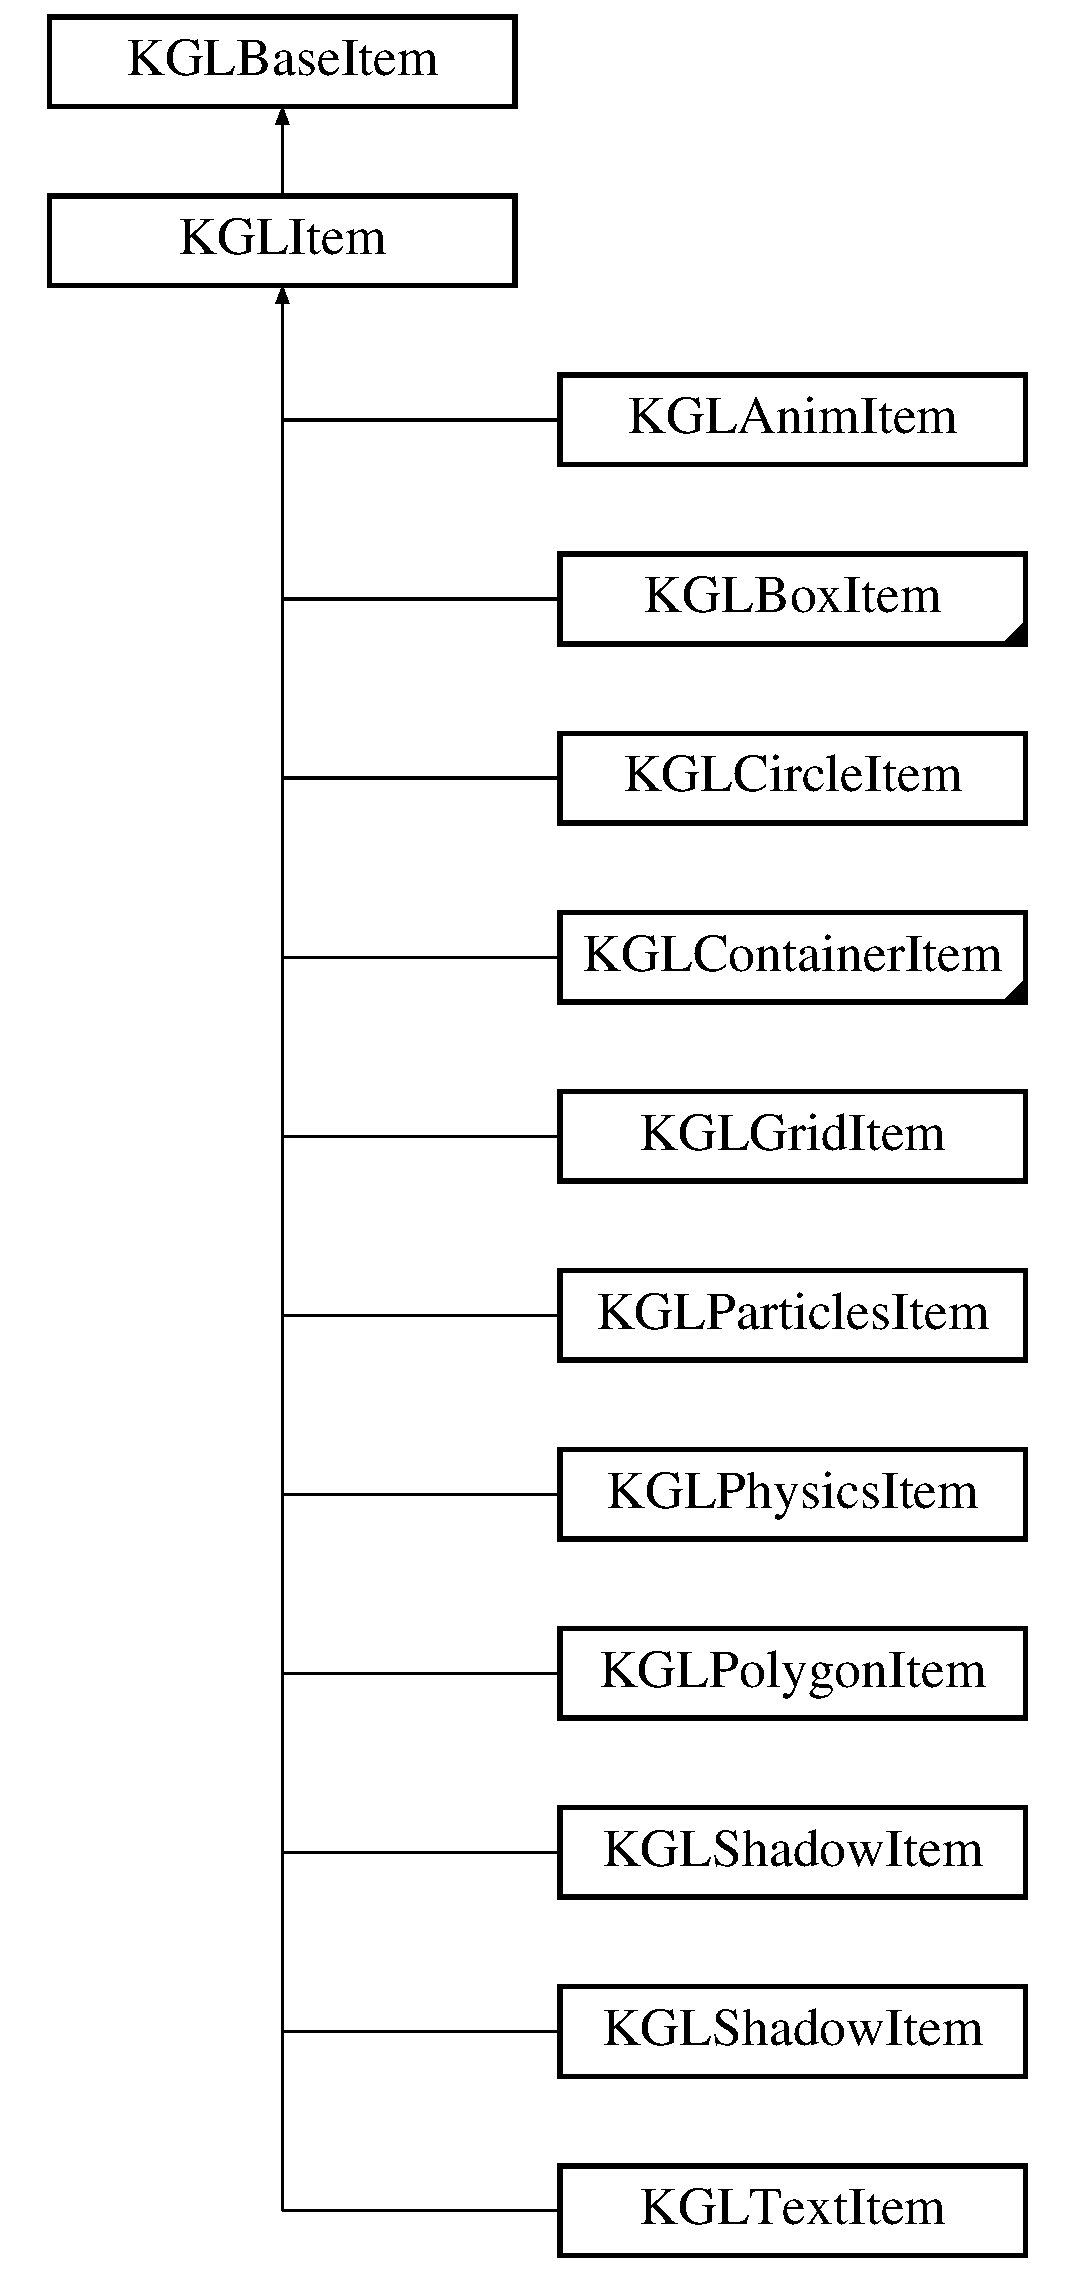
\includegraphics[height=12cm]{class_k_g_l_item}
\end{center}
\end{figure}
\subsection*{Signals}
\begin{CompactItemize}
\item 
void \hyperlink{class_k_g_l_item_9a6bf78a4509a1e38fc7be170ea0003e}{painted} ()
\end{CompactItemize}
\subsection*{Public Member Functions}
\begin{CompactItemize}
\item 
virtual void \hyperlink{class_k_g_l_item_4e4766cf0362fa050bffdf5f45d6d13f}{draw} ()
\item 
virtual void \hyperlink{class_k_g_l_item_3dbecc9db8e526a4c9623b35a004ed3c}{updateTransform} ()
\item 
\hyperlink{class_k_g_l_item_5ccd50011902e82584b676c5ffd6d5c0}{KGLItem} (\hyperlink{class_k_g_l_engine}{KGLEngine} $\ast$parent=0)
\item 
\hyperlink{class_k_g_l_item_0c2b3f2c4ee76fb09d58e95d75a0f12f}{KGLItem} (const QPolygonF \&poly, \hyperlink{class_k_g_l_engine}{KGLEngine} $\ast$parent=0)
\item 
\hyperlink{class_k_g_l_item_6a49457d29817772b0c05f471f3e8777}{KGLItem} (const QSizeF \&box, \hyperlink{class_k_g_l_engine}{KGLEngine} $\ast$parent=0)
\item 
\hyperlink{class_k_g_l_item_f1a9f58e453406da21e2db2e8a76bda1}{KGLItem} (const QLineF \&line, \hyperlink{class_k_g_l_engine}{KGLEngine} $\ast$parent=0)
\item 
\hyperlink{class_k_g_l_item}{KGLItem} $\ast$ \hyperlink{class_k_g_l_item_59c3205b918efb873fb011d4b676d2cd}{clone} ()
\item 
void \hyperlink{class_k_g_l_item_a667143176d94fd2366c64cd5d34b46e}{addChildItem} (\hyperlink{class_k_g_l_item}{KGLItem} $\ast$item)
\item 
void \hyperlink{class_k_g_l_item_42b7c5842dc8e7ee01c46b2a767e021a}{remChildItem} (\hyperlink{class_k_g_l_item}{KGLItem} $\ast$item)
\item 
\hyperlink{class_k_g_l_item_a303f5bf35c176400181aa59e3093ffa}{$\sim$KGLItem} ()
\item 
void \hyperlink{class_k_g_l_item_333a6829b561f2d9a5f904712aa3e3ed}{setMode} (GLenum m)
\item 
void \hyperlink{class_k_g_l_item_2ae8380935a0e01b35260dbb264270d5}{setTexture} (const GLuint \&t)
\item 
void \hyperlink{class_k_g_l_item_bf848a33d55dd5f96cd2399abe79411c}{setTexture} (\hyperlink{class_k_g_l_texture}{KGLTexture} $\ast$t)
\item 
void \hyperlink{class_k_g_l_item_73e87ddc6624de761a908880ab63bd77}{setTexture} (const QString \&fileName)
\item 
void \hyperlink{class_k_g_l_item_c68ff3db4cf505a10c1f95dbb24b3d8e}{setTexture} (const QImage \&image)
\item 
void \hyperlink{class_k_g_l_item_3cf5a12787e3a1be3695a4a2460b9f0d}{setTexture} (const QPixmap \&pix)
\item 
void \hyperlink{class_k_g_l_item_ccd2a4bf039b7274a0df572bd341d2d9}{setColor} (const QColor \&c)
\item 
void \hyperlink{class_k_g_l_item_0e29a2ca6924be0e2c950fd5c764fdab}{setAlpha} (const float \&a)
\item 
void \hyperlink{class_k_g_l_item_f1bec83ac3d7ad0a43cee9253d482343}{showBoundingBox} (bool b)
\item 
void \hyperlink{class_k_g_l_item_defcc7f3930968a04620e378fa7ba2b6}{showCenter} (bool b)
\item 
void \hyperlink{class_k_g_l_item_e3f2d07953ada32dafa43b48a3062677}{setTextureEnable} (bool t)
\item 
void \hyperlink{class_k_g_l_item_d615added4952e9d4e386ab8606872d6}{setProgram} (\hyperlink{class_k_g_l_program}{KGLProgram} $\ast$p)
\item 
\hyperlink{class_k_g_l_texture}{KGLTexture} $\ast$ \hyperlink{class_k_g_l_item_d5e6b6171894e455e36994b76ccb7f97}{texture} ()
\item 
\hyperlink{class_k_g_l_program}{KGLProgram} $\ast$ \hyperlink{class_k_g_l_item_3d4fca70cb1b6c9fab99b02696c50ca0}{program} ()
\item 
const QColor \& \hyperlink{class_k_g_l_item_cc12f268b3573be5aa6cb9aeb64723aa}{color} ()
\item 
const float \& \hyperlink{class_k_g_l_item_b9e32117300fa687fa861903af862731}{alpha} ()
\item 
QList$<$ \hyperlink{class_k_g_l_item}{KGLItem} $\ast$ $>$ \hyperlink{class_k_g_l_item_1dcc73984997f926f8188663f2e98443}{childItems} ()
\end{CompactItemize}
\subsection*{Protected Member Functions}
\begin{CompactItemize}
\item 
virtual void \hyperlink{class_k_g_l_item_bf80656de9729f6e5c0519ecb1a2301b}{create} ()
\item 
void \hyperlink{class_k_g_l_item_492b385411549f646d1278db59706779}{drawChild} ()
\item 
void \hyperlink{class_k_g_l_item_2227b986b72366e149815a5fa5838d52}{init} ()
\item 
virtual void \hyperlink{class_k_g_l_item_1d33b3aacc34428bc199771a90b00bc0}{drawGLPoint} (\hyperlink{class_k_g_l_point}{KGLPoint} \&p)
\item 
virtual void \hyperlink{class_k_g_l_item_6b5f40aeec53896189e8dd4f8fefb76b}{drawBoundingBox} ()
\item 
virtual void \hyperlink{class_k_g_l_item_ff61febb3b171446aacf3c6c947fa475}{drawCenter} ()
\end{CompactItemize}


\subsection{Constructor \& Destructor Documentation}
\hypertarget{class_k_g_l_item_5ccd50011902e82584b676c5ffd6d5c0}{
\index{KGLItem@{KGLItem}!KGLItem@{KGLItem}}
\index{KGLItem@{KGLItem}!KGLItem@{KGLItem}}
\subsubsection[{KGLItem}]{\setlength{\rightskip}{0pt plus 5cm}KGLItem::KGLItem ({\bf KGLEngine} $\ast$ {\em parent} = {\tt 0})\hspace{0.3cm}{\tt  \mbox{[}explicit\mbox{]}}}}
\label{class_k_g_l_item_5ccd50011902e82584b676c5ffd6d5c0}


\hypertarget{class_k_g_l_item_0c2b3f2c4ee76fb09d58e95d75a0f12f}{
\index{KGLItem@{KGLItem}!KGLItem@{KGLItem}}
\index{KGLItem@{KGLItem}!KGLItem@{KGLItem}}
\subsubsection[{KGLItem}]{\setlength{\rightskip}{0pt plus 5cm}KGLItem::KGLItem (const QPolygonF \& {\em poly}, \/  {\bf KGLEngine} $\ast$ {\em parent} = {\tt 0})\hspace{0.3cm}{\tt  \mbox{[}explicit\mbox{]}}}}
\label{class_k_g_l_item_0c2b3f2c4ee76fb09d58e95d75a0f12f}


\hypertarget{class_k_g_l_item_6a49457d29817772b0c05f471f3e8777}{
\index{KGLItem@{KGLItem}!KGLItem@{KGLItem}}
\index{KGLItem@{KGLItem}!KGLItem@{KGLItem}}
\subsubsection[{KGLItem}]{\setlength{\rightskip}{0pt plus 5cm}KGLItem::KGLItem (const QSizeF \& {\em box}, \/  {\bf KGLEngine} $\ast$ {\em parent} = {\tt 0})\hspace{0.3cm}{\tt  \mbox{[}explicit\mbox{]}}}}
\label{class_k_g_l_item_6a49457d29817772b0c05f471f3e8777}


\hypertarget{class_k_g_l_item_f1a9f58e453406da21e2db2e8a76bda1}{
\index{KGLItem@{KGLItem}!KGLItem@{KGLItem}}
\index{KGLItem@{KGLItem}!KGLItem@{KGLItem}}
\subsubsection[{KGLItem}]{\setlength{\rightskip}{0pt plus 5cm}KGLItem::KGLItem (const QLineF \& {\em line}, \/  {\bf KGLEngine} $\ast$ {\em parent} = {\tt 0})\hspace{0.3cm}{\tt  \mbox{[}explicit\mbox{]}}}}
\label{class_k_g_l_item_f1a9f58e453406da21e2db2e8a76bda1}


\hypertarget{class_k_g_l_item_a303f5bf35c176400181aa59e3093ffa}{
\index{KGLItem@{KGLItem}!$\sim$KGLItem@{$\sim$KGLItem}}
\index{$\sim$KGLItem@{$\sim$KGLItem}!KGLItem@{KGLItem}}
\subsubsection[{$\sim$KGLItem}]{\setlength{\rightskip}{0pt plus 5cm}KGLItem::$\sim$KGLItem ()}}
\label{class_k_g_l_item_a303f5bf35c176400181aa59e3093ffa}




\subsection{Member Function Documentation}
\hypertarget{class_k_g_l_item_a667143176d94fd2366c64cd5d34b46e}{
\index{KGLItem@{KGLItem}!addChildItem@{addChildItem}}
\index{addChildItem@{addChildItem}!KGLItem@{KGLItem}}
\subsubsection[{addChildItem}]{\setlength{\rightskip}{0pt plus 5cm}void KGLItem::addChildItem ({\bf KGLItem} $\ast$ {\em item})\hspace{0.3cm}{\tt  \mbox{[}inline\mbox{]}}}}
\label{class_k_g_l_item_a667143176d94fd2366c64cd5d34b46e}


\hypertarget{class_k_g_l_item_b9e32117300fa687fa861903af862731}{
\index{KGLItem@{KGLItem}!alpha@{alpha}}
\index{alpha@{alpha}!KGLItem@{KGLItem}}
\subsubsection[{alpha}]{\setlength{\rightskip}{0pt plus 5cm}const float\& KGLItem::alpha ()\hspace{0.3cm}{\tt  \mbox{[}inline\mbox{]}}}}
\label{class_k_g_l_item_b9e32117300fa687fa861903af862731}


\hypertarget{class_k_g_l_item_1dcc73984997f926f8188663f2e98443}{
\index{KGLItem@{KGLItem}!childItems@{childItems}}
\index{childItems@{childItems}!KGLItem@{KGLItem}}
\subsubsection[{childItems}]{\setlength{\rightskip}{0pt plus 5cm}QList$<${\bf KGLItem}$\ast$$>$ KGLItem::childItems ()\hspace{0.3cm}{\tt  \mbox{[}inline\mbox{]}}}}
\label{class_k_g_l_item_1dcc73984997f926f8188663f2e98443}


\hypertarget{class_k_g_l_item_59c3205b918efb873fb011d4b676d2cd}{
\index{KGLItem@{KGLItem}!clone@{clone}}
\index{clone@{clone}!KGLItem@{KGLItem}}
\subsubsection[{clone}]{\setlength{\rightskip}{0pt plus 5cm}{\bf KGLItem} $\ast$ KGLItem::clone ()}}
\label{class_k_g_l_item_59c3205b918efb873fb011d4b676d2cd}


\hypertarget{class_k_g_l_item_cc12f268b3573be5aa6cb9aeb64723aa}{
\index{KGLItem@{KGLItem}!color@{color}}
\index{color@{color}!KGLItem@{KGLItem}}
\subsubsection[{color}]{\setlength{\rightskip}{0pt plus 5cm}const QColor\& KGLItem::color ()\hspace{0.3cm}{\tt  \mbox{[}inline\mbox{]}}}}
\label{class_k_g_l_item_cc12f268b3573be5aa6cb9aeb64723aa}


\hypertarget{class_k_g_l_item_bf80656de9729f6e5c0519ecb1a2301b}{
\index{KGLItem@{KGLItem}!create@{create}}
\index{create@{create}!KGLItem@{KGLItem}}
\subsubsection[{create}]{\setlength{\rightskip}{0pt plus 5cm}void KGLItem::create ()\hspace{0.3cm}{\tt  \mbox{[}protected, virtual\mbox{]}}}}
\label{class_k_g_l_item_bf80656de9729f6e5c0519ecb1a2301b}


\hypertarget{class_k_g_l_item_4e4766cf0362fa050bffdf5f45d6d13f}{
\index{KGLItem@{KGLItem}!draw@{draw}}
\index{draw@{draw}!KGLItem@{KGLItem}}
\subsubsection[{draw}]{\setlength{\rightskip}{0pt plus 5cm}void KGLItem::draw ()\hspace{0.3cm}{\tt  \mbox{[}virtual\mbox{]}}}}
\label{class_k_g_l_item_4e4766cf0362fa050bffdf5f45d6d13f}




Reimplemented in \hyperlink{class_k_g_l_shadow_item_97433b863559d8f38199fe68a5b21bcc}{KGLShadowItem}, \hyperlink{class_k_g_l_container_item_a785dc67935db5f335c74e4a7fb685b9}{KGLContainerItem}, \hyperlink{class_k_g_l_particles_item_ce6df2f63f0566993f075f7ce55bb714}{KGLParticlesItem}, and \hyperlink{class_k_g_l_shadow_item_97433b863559d8f38199fe68a5b21bcc}{KGLShadowItem}.\hypertarget{class_k_g_l_item_6b5f40aeec53896189e8dd4f8fefb76b}{
\index{KGLItem@{KGLItem}!drawBoundingBox@{drawBoundingBox}}
\index{drawBoundingBox@{drawBoundingBox}!KGLItem@{KGLItem}}
\subsubsection[{drawBoundingBox}]{\setlength{\rightskip}{0pt plus 5cm}void KGLItem::drawBoundingBox ()\hspace{0.3cm}{\tt  \mbox{[}protected, virtual\mbox{]}}}}
\label{class_k_g_l_item_6b5f40aeec53896189e8dd4f8fefb76b}


\hypertarget{class_k_g_l_item_ff61febb3b171446aacf3c6c947fa475}{
\index{KGLItem@{KGLItem}!drawCenter@{drawCenter}}
\index{drawCenter@{drawCenter}!KGLItem@{KGLItem}}
\subsubsection[{drawCenter}]{\setlength{\rightskip}{0pt plus 5cm}void KGLItem::drawCenter ()\hspace{0.3cm}{\tt  \mbox{[}protected, virtual\mbox{]}}}}
\label{class_k_g_l_item_ff61febb3b171446aacf3c6c947fa475}


\hypertarget{class_k_g_l_item_492b385411549f646d1278db59706779}{
\index{KGLItem@{KGLItem}!drawChild@{drawChild}}
\index{drawChild@{drawChild}!KGLItem@{KGLItem}}
\subsubsection[{drawChild}]{\setlength{\rightskip}{0pt plus 5cm}void KGLItem::drawChild ()\hspace{0.3cm}{\tt  \mbox{[}protected\mbox{]}}}}
\label{class_k_g_l_item_492b385411549f646d1278db59706779}


\hypertarget{class_k_g_l_item_1d33b3aacc34428bc199771a90b00bc0}{
\index{KGLItem@{KGLItem}!drawGLPoint@{drawGLPoint}}
\index{drawGLPoint@{drawGLPoint}!KGLItem@{KGLItem}}
\subsubsection[{drawGLPoint}]{\setlength{\rightskip}{0pt plus 5cm}void KGLItem::drawGLPoint ({\bf KGLPoint} \& {\em p})\hspace{0.3cm}{\tt  \mbox{[}protected, virtual\mbox{]}}}}
\label{class_k_g_l_item_1d33b3aacc34428bc199771a90b00bc0}


\hypertarget{class_k_g_l_item_2227b986b72366e149815a5fa5838d52}{
\index{KGLItem@{KGLItem}!init@{init}}
\index{init@{init}!KGLItem@{KGLItem}}
\subsubsection[{init}]{\setlength{\rightskip}{0pt plus 5cm}void KGLItem::init ()\hspace{0.3cm}{\tt  \mbox{[}protected\mbox{]}}}}
\label{class_k_g_l_item_2227b986b72366e149815a5fa5838d52}




Reimplemented in \hyperlink{class_k_g_l_grid_item_b86b8c2552de5956e79abb6b0ce81d73}{KGLGridItem}.\hypertarget{class_k_g_l_item_9a6bf78a4509a1e38fc7be170ea0003e}{
\index{KGLItem@{KGLItem}!painted@{painted}}
\index{painted@{painted}!KGLItem@{KGLItem}}
\subsubsection[{painted}]{\setlength{\rightskip}{0pt plus 5cm}void KGLItem::painted ()\hspace{0.3cm}{\tt  \mbox{[}signal\mbox{]}}}}
\label{class_k_g_l_item_9a6bf78a4509a1e38fc7be170ea0003e}


\hypertarget{class_k_g_l_item_3d4fca70cb1b6c9fab99b02696c50ca0}{
\index{KGLItem@{KGLItem}!program@{program}}
\index{program@{program}!KGLItem@{KGLItem}}
\subsubsection[{program}]{\setlength{\rightskip}{0pt plus 5cm}{\bf KGLProgram}$\ast$ KGLItem::program ()\hspace{0.3cm}{\tt  \mbox{[}inline\mbox{]}}}}
\label{class_k_g_l_item_3d4fca70cb1b6c9fab99b02696c50ca0}


\hypertarget{class_k_g_l_item_42b7c5842dc8e7ee01c46b2a767e021a}{
\index{KGLItem@{KGLItem}!remChildItem@{remChildItem}}
\index{remChildItem@{remChildItem}!KGLItem@{KGLItem}}
\subsubsection[{remChildItem}]{\setlength{\rightskip}{0pt plus 5cm}void KGLItem::remChildItem ({\bf KGLItem} $\ast$ {\em item})\hspace{0.3cm}{\tt  \mbox{[}inline\mbox{]}}}}
\label{class_k_g_l_item_42b7c5842dc8e7ee01c46b2a767e021a}


\hypertarget{class_k_g_l_item_0e29a2ca6924be0e2c950fd5c764fdab}{
\index{KGLItem@{KGLItem}!setAlpha@{setAlpha}}
\index{setAlpha@{setAlpha}!KGLItem@{KGLItem}}
\subsubsection[{setAlpha}]{\setlength{\rightskip}{0pt plus 5cm}void KGLItem::setAlpha (const float \& {\em a})}}
\label{class_k_g_l_item_0e29a2ca6924be0e2c950fd5c764fdab}


\hypertarget{class_k_g_l_item_ccd2a4bf039b7274a0df572bd341d2d9}{
\index{KGLItem@{KGLItem}!setColor@{setColor}}
\index{setColor@{setColor}!KGLItem@{KGLItem}}
\subsubsection[{setColor}]{\setlength{\rightskip}{0pt plus 5cm}void KGLItem::setColor (const QColor \& {\em c})}}
\label{class_k_g_l_item_ccd2a4bf039b7274a0df572bd341d2d9}


\hypertarget{class_k_g_l_item_333a6829b561f2d9a5f904712aa3e3ed}{
\index{KGLItem@{KGLItem}!setMode@{setMode}}
\index{setMode@{setMode}!KGLItem@{KGLItem}}
\subsubsection[{setMode}]{\setlength{\rightskip}{0pt plus 5cm}void KGLItem::setMode (GLenum {\em m})\hspace{0.3cm}{\tt  \mbox{[}inline\mbox{]}}}}
\label{class_k_g_l_item_333a6829b561f2d9a5f904712aa3e3ed}


\hypertarget{class_k_g_l_item_d615added4952e9d4e386ab8606872d6}{
\index{KGLItem@{KGLItem}!setProgram@{setProgram}}
\index{setProgram@{setProgram}!KGLItem@{KGLItem}}
\subsubsection[{setProgram}]{\setlength{\rightskip}{0pt plus 5cm}void KGLItem::setProgram ({\bf KGLProgram} $\ast$ {\em p})\hspace{0.3cm}{\tt  \mbox{[}inline\mbox{]}}}}
\label{class_k_g_l_item_d615added4952e9d4e386ab8606872d6}


\hypertarget{class_k_g_l_item_3cf5a12787e3a1be3695a4a2460b9f0d}{
\index{KGLItem@{KGLItem}!setTexture@{setTexture}}
\index{setTexture@{setTexture}!KGLItem@{KGLItem}}
\subsubsection[{setTexture}]{\setlength{\rightskip}{0pt plus 5cm}void KGLItem::setTexture (const QPixmap \& {\em pix})\hspace{0.3cm}{\tt  \mbox{[}inline\mbox{]}}}}
\label{class_k_g_l_item_3cf5a12787e3a1be3695a4a2460b9f0d}


\hypertarget{class_k_g_l_item_c68ff3db4cf505a10c1f95dbb24b3d8e}{
\index{KGLItem@{KGLItem}!setTexture@{setTexture}}
\index{setTexture@{setTexture}!KGLItem@{KGLItem}}
\subsubsection[{setTexture}]{\setlength{\rightskip}{0pt plus 5cm}void KGLItem::setTexture (const QImage \& {\em image})\hspace{0.3cm}{\tt  \mbox{[}inline\mbox{]}}}}
\label{class_k_g_l_item_c68ff3db4cf505a10c1f95dbb24b3d8e}


\hypertarget{class_k_g_l_item_73e87ddc6624de761a908880ab63bd77}{
\index{KGLItem@{KGLItem}!setTexture@{setTexture}}
\index{setTexture@{setTexture}!KGLItem@{KGLItem}}
\subsubsection[{setTexture}]{\setlength{\rightskip}{0pt plus 5cm}void KGLItem::setTexture (const QString \& {\em fileName})\hspace{0.3cm}{\tt  \mbox{[}inline\mbox{]}}}}
\label{class_k_g_l_item_73e87ddc6624de761a908880ab63bd77}


\hypertarget{class_k_g_l_item_bf848a33d55dd5f96cd2399abe79411c}{
\index{KGLItem@{KGLItem}!setTexture@{setTexture}}
\index{setTexture@{setTexture}!KGLItem@{KGLItem}}
\subsubsection[{setTexture}]{\setlength{\rightskip}{0pt plus 5cm}void KGLItem::setTexture ({\bf KGLTexture} $\ast$ {\em t})\hspace{0.3cm}{\tt  \mbox{[}inline\mbox{]}}}}
\label{class_k_g_l_item_bf848a33d55dd5f96cd2399abe79411c}


\hypertarget{class_k_g_l_item_2ae8380935a0e01b35260dbb264270d5}{
\index{KGLItem@{KGLItem}!setTexture@{setTexture}}
\index{setTexture@{setTexture}!KGLItem@{KGLItem}}
\subsubsection[{setTexture}]{\setlength{\rightskip}{0pt plus 5cm}void KGLItem::setTexture (const GLuint \& {\em t})\hspace{0.3cm}{\tt  \mbox{[}inline\mbox{]}}}}
\label{class_k_g_l_item_2ae8380935a0e01b35260dbb264270d5}


\hypertarget{class_k_g_l_item_e3f2d07953ada32dafa43b48a3062677}{
\index{KGLItem@{KGLItem}!setTextureEnable@{setTextureEnable}}
\index{setTextureEnable@{setTextureEnable}!KGLItem@{KGLItem}}
\subsubsection[{setTextureEnable}]{\setlength{\rightskip}{0pt plus 5cm}void KGLItem::setTextureEnable (bool {\em t})\hspace{0.3cm}{\tt  \mbox{[}inline\mbox{]}}}}
\label{class_k_g_l_item_e3f2d07953ada32dafa43b48a3062677}


\hypertarget{class_k_g_l_item_f1bec83ac3d7ad0a43cee9253d482343}{
\index{KGLItem@{KGLItem}!showBoundingBox@{showBoundingBox}}
\index{showBoundingBox@{showBoundingBox}!KGLItem@{KGLItem}}
\subsubsection[{showBoundingBox}]{\setlength{\rightskip}{0pt plus 5cm}void KGLItem::showBoundingBox (bool {\em b})\hspace{0.3cm}{\tt  \mbox{[}inline\mbox{]}}}}
\label{class_k_g_l_item_f1bec83ac3d7ad0a43cee9253d482343}


\hypertarget{class_k_g_l_item_defcc7f3930968a04620e378fa7ba2b6}{
\index{KGLItem@{KGLItem}!showCenter@{showCenter}}
\index{showCenter@{showCenter}!KGLItem@{KGLItem}}
\subsubsection[{showCenter}]{\setlength{\rightskip}{0pt plus 5cm}void KGLItem::showCenter (bool {\em b})\hspace{0.3cm}{\tt  \mbox{[}inline\mbox{]}}}}
\label{class_k_g_l_item_defcc7f3930968a04620e378fa7ba2b6}


\hypertarget{class_k_g_l_item_d5e6b6171894e455e36994b76ccb7f97}{
\index{KGLItem@{KGLItem}!texture@{texture}}
\index{texture@{texture}!KGLItem@{KGLItem}}
\subsubsection[{texture}]{\setlength{\rightskip}{0pt plus 5cm}{\bf KGLTexture}$\ast$ KGLItem::texture ()\hspace{0.3cm}{\tt  \mbox{[}inline\mbox{]}}}}
\label{class_k_g_l_item_d5e6b6171894e455e36994b76ccb7f97}


\hypertarget{class_k_g_l_item_3dbecc9db8e526a4c9623b35a004ed3c}{
\index{KGLItem@{KGLItem}!updateTransform@{updateTransform}}
\index{updateTransform@{updateTransform}!KGLItem@{KGLItem}}
\subsubsection[{updateTransform}]{\setlength{\rightskip}{0pt plus 5cm}void KGLItem::updateTransform ()\hspace{0.3cm}{\tt  \mbox{[}virtual\mbox{]}}}}
\label{class_k_g_l_item_3dbecc9db8e526a4c9623b35a004ed3c}




Reimplemented from \hyperlink{class_k_g_l_base_item_6e020830d4452864cdb6c8fea4531e0d}{KGLBaseItem}.

The documentation for this class was generated from the following files:\begin{CompactItemize}
\item 
/home/sacha/programmation/gluon/kgl/\hyperlink{kglitem_8h}{kglitem.h}\item 
/home/sacha/programmation/gluon/kgl/\hyperlink{kglitem_8cpp}{kglitem.cpp}\end{CompactItemize}

\hypertarget{class_k_g_l_item_list}{
\section{KGLItemList Class Reference}
\label{class_k_g_l_item_list}\index{KGLItemList@{KGLItemList}}
}
{\tt \#include $<$kglitemlist.h$>$}

\subsection*{Public Member Functions}
\begin{CompactItemize}
\item 
\hyperlink{class_k_g_l_item_list_35d6828d5eb488bb0406cf59062ef2d0}{KGLItemList} ()
\item 
\hyperlink{class_k_g_l_item_list_30ab7b44c5350a240ec5bb4375ad44b1}{$\sim$KGLItemList} ()
\end{CompactItemize}


\subsection{Constructor \& Destructor Documentation}
\hypertarget{class_k_g_l_item_list_35d6828d5eb488bb0406cf59062ef2d0}{
\index{KGLItemList@{KGLItemList}!KGLItemList@{KGLItemList}}
\index{KGLItemList@{KGLItemList}!KGLItemList@{KGLItemList}}
\subsubsection[{KGLItemList}]{\setlength{\rightskip}{0pt plus 5cm}KGLItemList::KGLItemList ()}}
\label{class_k_g_l_item_list_35d6828d5eb488bb0406cf59062ef2d0}


\hypertarget{class_k_g_l_item_list_30ab7b44c5350a240ec5bb4375ad44b1}{
\index{KGLItemList@{KGLItemList}!$\sim$KGLItemList@{$\sim$KGLItemList}}
\index{$\sim$KGLItemList@{$\sim$KGLItemList}!KGLItemList@{KGLItemList}}
\subsubsection[{$\sim$KGLItemList}]{\setlength{\rightskip}{0pt plus 5cm}KGLItemList::$\sim$KGLItemList ()}}
\label{class_k_g_l_item_list_30ab7b44c5350a240ec5bb4375ad44b1}




The documentation for this class was generated from the following files:\begin{CompactItemize}
\item 
/home/sacha/programmation/gluon/kgl/\hyperlink{kglitemlist_8h}{kglitemlist.h}\item 
/home/sacha/programmation/gluon/kgl/\hyperlink{kglitemlist_8cpp}{kglitemlist.cpp}\end{CompactItemize}

\hypertarget{class_k_g_l_light_fx}{
\section{KGLLightFx Class Reference}
\label{class_k_g_l_light_fx}\index{KGLLightFx@{KGLLightFx}}
}
{\tt \#include $<$kglfx.h$>$}

Inheritance diagram for KGLLightFx::\begin{figure}[H]
\begin{center}
\leavevmode
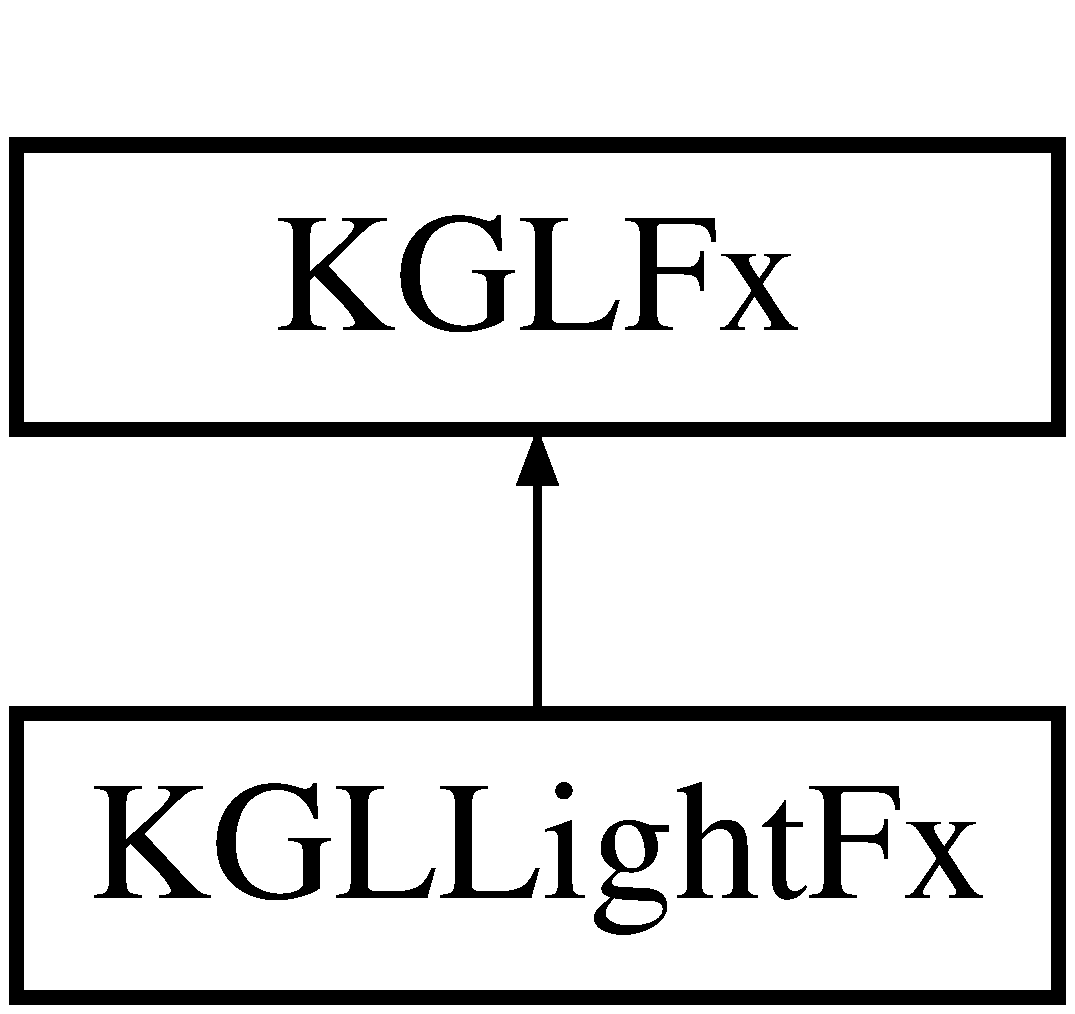
\includegraphics[height=2cm]{class_k_g_l_light_fx}
\end{center}
\end{figure}
\subsection*{Public Member Functions}
\begin{CompactItemize}
\item 
\hyperlink{class_k_g_l_light_fx_ef8e2da38e34d652c53c91f8becf0e60}{KGLLightFx} ()
\item 
void \hyperlink{class_k_g_l_light_fx_247efd2e5d7ba3e4db7163b32d3b7d77}{setLight} (float l)
\end{CompactItemize}


\subsection{Constructor \& Destructor Documentation}
\hypertarget{class_k_g_l_light_fx_ef8e2da38e34d652c53c91f8becf0e60}{
\index{KGLLightFx@{KGLLightFx}!KGLLightFx@{KGLLightFx}}
\index{KGLLightFx@{KGLLightFx}!KGLLightFx@{KGLLightFx}}
\subsubsection[{KGLLightFx}]{\setlength{\rightskip}{0pt plus 5cm}KGLLightFx::KGLLightFx ()}}
\label{class_k_g_l_light_fx_ef8e2da38e34d652c53c91f8becf0e60}




\subsection{Member Function Documentation}
\hypertarget{class_k_g_l_light_fx_247efd2e5d7ba3e4db7163b32d3b7d77}{
\index{KGLLightFx@{KGLLightFx}!setLight@{setLight}}
\index{setLight@{setLight}!KGLLightFx@{KGLLightFx}}
\subsubsection[{setLight}]{\setlength{\rightskip}{0pt plus 5cm}void KGLLightFx::setLight (float {\em l})\hspace{0.3cm}{\tt  \mbox{[}inline\mbox{]}}}}
\label{class_k_g_l_light_fx_247efd2e5d7ba3e4db7163b32d3b7d77}




The documentation for this class was generated from the following files:\begin{CompactItemize}
\item 
/home/sacha/programmation/gluon/kgl/\hyperlink{kglfx_8h}{kglfx.h}\item 
/home/sacha/programmation/gluon/kgl/\hyperlink{kglfx_8cpp}{kglfx.cpp}\end{CompactItemize}

\hypertarget{class_k_g_l_particle}{
\section{KGLParticle Class Reference}
\label{class_k_g_l_particle}\index{KGLParticle@{KGLParticle}}
}
{\tt \#include $<$kglparticlesitem.h$>$}

\subsection*{Public Member Functions}
\begin{CompactItemize}
\item 
\hyperlink{class_k_g_l_particle_0b2a6cb94ef297c99e6471dd91a1376d}{KGLParticle} ()
\item 
void \hyperlink{class_k_g_l_particle_810f22cab6cd83fb40175c07976d97f5}{init} ()
\item 
void \hyperlink{class_k_g_l_particle_5e7afc417a0368d3b1b05973782267e7}{move} ()
\item 
void \hyperlink{class_k_g_l_particle_28a0fed37487b9b14f822b5b30ff5e09}{reset} ()
\item 
void \hyperlink{class_k_g_l_particle_e4f6170615e9a4318b71e54146e81bb5}{setColor} (const QColor \&col)
\item 
void \hyperlink{class_k_g_l_particle_0cbaf806d3692135ff4a874b0c9e0cfc}{setColorStep} (const QColor \&c)
\item 
void \hyperlink{class_k_g_l_particle_e760126a7614c2f9e353354159125a3a}{setPosition} (const QPointF \&p)
\item 
void \hyperlink{class_k_g_l_particle_28b82ab43a56e3016477e9b42c334bda}{setInitPosition} (const QPointF \&p)
\item 
void \hyperlink{class_k_g_l_particle_c2e395f657d6bac641bbd4b3e34e6304}{setDirection} (const QPointF \&d)
\item 
void \hyperlink{class_k_g_l_particle_4d17097516ffa4248e359c14e3b8d3dc}{setSpeed} (const float \&s)
\item 
void \hyperlink{class_k_g_l_particle_7eac7336cf145c7b2f53e239d63734f4}{setSize} (const float \&s)
\item 
void \hyperlink{class_k_g_l_particle_4ad871207f00236ff4aef3711710771f}{setAlpha} (const float \&a)
\item 
void \hyperlink{class_k_g_l_particle_410d9b3a43554f25386763f3a1800eeb}{setAlphaStep} (const float \&s)
\item 
void \hyperlink{class_k_g_l_particle_47978679ec7686a3031bc429eb3079b7}{setTexture} (const QString \&name)
\item 
void \hyperlink{class_k_g_l_particle_ff9e1c4f5c6d3a8a26f1a30e59a0e48b}{setTexture} (const QPixmap \&name)
\item 
void \hyperlink{class_k_g_l_particle_02f5c7f2b11ac94573570af130d0fe33}{setTexture} (\hyperlink{class_k_g_l_texture}{KGLTexture} $\ast$t)
\item 
const QPointF \& \hyperlink{class_k_g_l_particle_7fd9f005de276e58245475175b23b2e2}{position} ()
\item 
const float \& \hyperlink{class_k_g_l_particle_8597d2785cedd9cb5bb40b7d45510e07}{size} ()
\item 
const float \& \hyperlink{class_k_g_l_particle_82f20a264844ee28b6add85a5cb3842c}{alpha} ()
\item 
const QColor \& \hyperlink{class_k_g_l_particle_b9f25fd03e317c0125fde5c57674eebe}{color} ()
\item 
const QPointF \& \hyperlink{class_k_g_l_particle_5dd92029982c4c3fd095f089626b6650}{direction} ()
\item 
const float \& \hyperlink{class_k_g_l_particle_1a612ce49af0dd6dc80ff224ee9fd2d8}{speed} ()
\item 
\hyperlink{class_k_g_l_texture}{KGLTexture} $\ast$ \hyperlink{class_k_g_l_particle_f6e6914d833ff48e1b6ee719a5b15962}{tex} ()
\end{CompactItemize}


\subsection{Constructor \& Destructor Documentation}
\hypertarget{class_k_g_l_particle_0b2a6cb94ef297c99e6471dd91a1376d}{
\index{KGLParticle@{KGLParticle}!KGLParticle@{KGLParticle}}
\index{KGLParticle@{KGLParticle}!KGLParticle@{KGLParticle}}
\subsubsection[{KGLParticle}]{\setlength{\rightskip}{0pt plus 5cm}KGLParticle::KGLParticle ()}}
\label{class_k_g_l_particle_0b2a6cb94ef297c99e6471dd91a1376d}




\subsection{Member Function Documentation}
\hypertarget{class_k_g_l_particle_82f20a264844ee28b6add85a5cb3842c}{
\index{KGLParticle@{KGLParticle}!alpha@{alpha}}
\index{alpha@{alpha}!KGLParticle@{KGLParticle}}
\subsubsection[{alpha}]{\setlength{\rightskip}{0pt plus 5cm}const float\& KGLParticle::alpha ()\hspace{0.3cm}{\tt  \mbox{[}inline\mbox{]}}}}
\label{class_k_g_l_particle_82f20a264844ee28b6add85a5cb3842c}


\hypertarget{class_k_g_l_particle_b9f25fd03e317c0125fde5c57674eebe}{
\index{KGLParticle@{KGLParticle}!color@{color}}
\index{color@{color}!KGLParticle@{KGLParticle}}
\subsubsection[{color}]{\setlength{\rightskip}{0pt plus 5cm}const QColor\& KGLParticle::color ()\hspace{0.3cm}{\tt  \mbox{[}inline\mbox{]}}}}
\label{class_k_g_l_particle_b9f25fd03e317c0125fde5c57674eebe}


\hypertarget{class_k_g_l_particle_5dd92029982c4c3fd095f089626b6650}{
\index{KGLParticle@{KGLParticle}!direction@{direction}}
\index{direction@{direction}!KGLParticle@{KGLParticle}}
\subsubsection[{direction}]{\setlength{\rightskip}{0pt plus 5cm}const QPointF\& KGLParticle::direction ()\hspace{0.3cm}{\tt  \mbox{[}inline\mbox{]}}}}
\label{class_k_g_l_particle_5dd92029982c4c3fd095f089626b6650}


\hypertarget{class_k_g_l_particle_810f22cab6cd83fb40175c07976d97f5}{
\index{KGLParticle@{KGLParticle}!init@{init}}
\index{init@{init}!KGLParticle@{KGLParticle}}
\subsubsection[{init}]{\setlength{\rightskip}{0pt plus 5cm}void KGLParticle::init ()}}
\label{class_k_g_l_particle_810f22cab6cd83fb40175c07976d97f5}


\hypertarget{class_k_g_l_particle_5e7afc417a0368d3b1b05973782267e7}{
\index{KGLParticle@{KGLParticle}!move@{move}}
\index{move@{move}!KGLParticle@{KGLParticle}}
\subsubsection[{move}]{\setlength{\rightskip}{0pt plus 5cm}void KGLParticle::move ()}}
\label{class_k_g_l_particle_5e7afc417a0368d3b1b05973782267e7}


\hypertarget{class_k_g_l_particle_7fd9f005de276e58245475175b23b2e2}{
\index{KGLParticle@{KGLParticle}!position@{position}}
\index{position@{position}!KGLParticle@{KGLParticle}}
\subsubsection[{position}]{\setlength{\rightskip}{0pt plus 5cm}const QPointF\& KGLParticle::position ()\hspace{0.3cm}{\tt  \mbox{[}inline\mbox{]}}}}
\label{class_k_g_l_particle_7fd9f005de276e58245475175b23b2e2}


\hypertarget{class_k_g_l_particle_28a0fed37487b9b14f822b5b30ff5e09}{
\index{KGLParticle@{KGLParticle}!reset@{reset}}
\index{reset@{reset}!KGLParticle@{KGLParticle}}
\subsubsection[{reset}]{\setlength{\rightskip}{0pt plus 5cm}void KGLParticle::reset ()\hspace{0.3cm}{\tt  \mbox{[}inline\mbox{]}}}}
\label{class_k_g_l_particle_28a0fed37487b9b14f822b5b30ff5e09}


\hypertarget{class_k_g_l_particle_4ad871207f00236ff4aef3711710771f}{
\index{KGLParticle@{KGLParticle}!setAlpha@{setAlpha}}
\index{setAlpha@{setAlpha}!KGLParticle@{KGLParticle}}
\subsubsection[{setAlpha}]{\setlength{\rightskip}{0pt plus 5cm}void KGLParticle::setAlpha (const float \& {\em a})\hspace{0.3cm}{\tt  \mbox{[}inline\mbox{]}}}}
\label{class_k_g_l_particle_4ad871207f00236ff4aef3711710771f}


\hypertarget{class_k_g_l_particle_410d9b3a43554f25386763f3a1800eeb}{
\index{KGLParticle@{KGLParticle}!setAlphaStep@{setAlphaStep}}
\index{setAlphaStep@{setAlphaStep}!KGLParticle@{KGLParticle}}
\subsubsection[{setAlphaStep}]{\setlength{\rightskip}{0pt plus 5cm}void KGLParticle::setAlphaStep (const float \& {\em s})\hspace{0.3cm}{\tt  \mbox{[}inline\mbox{]}}}}
\label{class_k_g_l_particle_410d9b3a43554f25386763f3a1800eeb}


\hypertarget{class_k_g_l_particle_e4f6170615e9a4318b71e54146e81bb5}{
\index{KGLParticle@{KGLParticle}!setColor@{setColor}}
\index{setColor@{setColor}!KGLParticle@{KGLParticle}}
\subsubsection[{setColor}]{\setlength{\rightskip}{0pt plus 5cm}void KGLParticle::setColor (const QColor \& {\em col})\hspace{0.3cm}{\tt  \mbox{[}inline\mbox{]}}}}
\label{class_k_g_l_particle_e4f6170615e9a4318b71e54146e81bb5}


\hypertarget{class_k_g_l_particle_0cbaf806d3692135ff4a874b0c9e0cfc}{
\index{KGLParticle@{KGLParticle}!setColorStep@{setColorStep}}
\index{setColorStep@{setColorStep}!KGLParticle@{KGLParticle}}
\subsubsection[{setColorStep}]{\setlength{\rightskip}{0pt plus 5cm}void KGLParticle::setColorStep (const QColor \& {\em c})\hspace{0.3cm}{\tt  \mbox{[}inline\mbox{]}}}}
\label{class_k_g_l_particle_0cbaf806d3692135ff4a874b0c9e0cfc}


\hypertarget{class_k_g_l_particle_c2e395f657d6bac641bbd4b3e34e6304}{
\index{KGLParticle@{KGLParticle}!setDirection@{setDirection}}
\index{setDirection@{setDirection}!KGLParticle@{KGLParticle}}
\subsubsection[{setDirection}]{\setlength{\rightskip}{0pt plus 5cm}void KGLParticle::setDirection (const QPointF \& {\em d})\hspace{0.3cm}{\tt  \mbox{[}inline\mbox{]}}}}
\label{class_k_g_l_particle_c2e395f657d6bac641bbd4b3e34e6304}


\hypertarget{class_k_g_l_particle_28b82ab43a56e3016477e9b42c334bda}{
\index{KGLParticle@{KGLParticle}!setInitPosition@{setInitPosition}}
\index{setInitPosition@{setInitPosition}!KGLParticle@{KGLParticle}}
\subsubsection[{setInitPosition}]{\setlength{\rightskip}{0pt plus 5cm}void KGLParticle::setInitPosition (const QPointF \& {\em p})\hspace{0.3cm}{\tt  \mbox{[}inline\mbox{]}}}}
\label{class_k_g_l_particle_28b82ab43a56e3016477e9b42c334bda}


\hypertarget{class_k_g_l_particle_e760126a7614c2f9e353354159125a3a}{
\index{KGLParticle@{KGLParticle}!setPosition@{setPosition}}
\index{setPosition@{setPosition}!KGLParticle@{KGLParticle}}
\subsubsection[{setPosition}]{\setlength{\rightskip}{0pt plus 5cm}void KGLParticle::setPosition (const QPointF \& {\em p})\hspace{0.3cm}{\tt  \mbox{[}inline\mbox{]}}}}
\label{class_k_g_l_particle_e760126a7614c2f9e353354159125a3a}


\hypertarget{class_k_g_l_particle_7eac7336cf145c7b2f53e239d63734f4}{
\index{KGLParticle@{KGLParticle}!setSize@{setSize}}
\index{setSize@{setSize}!KGLParticle@{KGLParticle}}
\subsubsection[{setSize}]{\setlength{\rightskip}{0pt plus 5cm}void KGLParticle::setSize (const float \& {\em s})\hspace{0.3cm}{\tt  \mbox{[}inline\mbox{]}}}}
\label{class_k_g_l_particle_7eac7336cf145c7b2f53e239d63734f4}


\hypertarget{class_k_g_l_particle_4d17097516ffa4248e359c14e3b8d3dc}{
\index{KGLParticle@{KGLParticle}!setSpeed@{setSpeed}}
\index{setSpeed@{setSpeed}!KGLParticle@{KGLParticle}}
\subsubsection[{setSpeed}]{\setlength{\rightskip}{0pt plus 5cm}void KGLParticle::setSpeed (const float \& {\em s})\hspace{0.3cm}{\tt  \mbox{[}inline\mbox{]}}}}
\label{class_k_g_l_particle_4d17097516ffa4248e359c14e3b8d3dc}


\hypertarget{class_k_g_l_particle_02f5c7f2b11ac94573570af130d0fe33}{
\index{KGLParticle@{KGLParticle}!setTexture@{setTexture}}
\index{setTexture@{setTexture}!KGLParticle@{KGLParticle}}
\subsubsection[{setTexture}]{\setlength{\rightskip}{0pt plus 5cm}void KGLParticle::setTexture ({\bf KGLTexture} $\ast$ {\em t})\hspace{0.3cm}{\tt  \mbox{[}inline\mbox{]}}}}
\label{class_k_g_l_particle_02f5c7f2b11ac94573570af130d0fe33}


\hypertarget{class_k_g_l_particle_ff9e1c4f5c6d3a8a26f1a30e59a0e48b}{
\index{KGLParticle@{KGLParticle}!setTexture@{setTexture}}
\index{setTexture@{setTexture}!KGLParticle@{KGLParticle}}
\subsubsection[{setTexture}]{\setlength{\rightskip}{0pt plus 5cm}void KGLParticle::setTexture (const QPixmap \& {\em name})\hspace{0.3cm}{\tt  \mbox{[}inline\mbox{]}}}}
\label{class_k_g_l_particle_ff9e1c4f5c6d3a8a26f1a30e59a0e48b}


\hypertarget{class_k_g_l_particle_47978679ec7686a3031bc429eb3079b7}{
\index{KGLParticle@{KGLParticle}!setTexture@{setTexture}}
\index{setTexture@{setTexture}!KGLParticle@{KGLParticle}}
\subsubsection[{setTexture}]{\setlength{\rightskip}{0pt plus 5cm}void KGLParticle::setTexture (const QString \& {\em name})\hspace{0.3cm}{\tt  \mbox{[}inline\mbox{]}}}}
\label{class_k_g_l_particle_47978679ec7686a3031bc429eb3079b7}


\hypertarget{class_k_g_l_particle_8597d2785cedd9cb5bb40b7d45510e07}{
\index{KGLParticle@{KGLParticle}!size@{size}}
\index{size@{size}!KGLParticle@{KGLParticle}}
\subsubsection[{size}]{\setlength{\rightskip}{0pt plus 5cm}const float\& KGLParticle::size ()\hspace{0.3cm}{\tt  \mbox{[}inline\mbox{]}}}}
\label{class_k_g_l_particle_8597d2785cedd9cb5bb40b7d45510e07}


\hypertarget{class_k_g_l_particle_1a612ce49af0dd6dc80ff224ee9fd2d8}{
\index{KGLParticle@{KGLParticle}!speed@{speed}}
\index{speed@{speed}!KGLParticle@{KGLParticle}}
\subsubsection[{speed}]{\setlength{\rightskip}{0pt plus 5cm}const float\& KGLParticle::speed ()\hspace{0.3cm}{\tt  \mbox{[}inline\mbox{]}}}}
\label{class_k_g_l_particle_1a612ce49af0dd6dc80ff224ee9fd2d8}


\hypertarget{class_k_g_l_particle_f6e6914d833ff48e1b6ee719a5b15962}{
\index{KGLParticle@{KGLParticle}!tex@{tex}}
\index{tex@{tex}!KGLParticle@{KGLParticle}}
\subsubsection[{tex}]{\setlength{\rightskip}{0pt plus 5cm}{\bf KGLTexture}$\ast$ KGLParticle::tex ()\hspace{0.3cm}{\tt  \mbox{[}inline\mbox{]}}}}
\label{class_k_g_l_particle_f6e6914d833ff48e1b6ee719a5b15962}




The documentation for this class was generated from the following files:\begin{CompactItemize}
\item 
/home/sacha/programmation/gluon/kgl/\hyperlink{kglparticlesitem_8h}{kglparticlesitem.h}\item 
/home/sacha/programmation/gluon/kgl/\hyperlink{kglparticlesitem_8cpp}{kglparticlesitem.cpp}\end{CompactItemize}

\hypertarget{class_k_g_l_particles_item}{
\section{KGLParticlesItem Class Reference}
\label{class_k_g_l_particles_item}\index{KGLParticlesItem@{KGLParticlesItem}}
}
{\tt \#include $<$kglparticlesitem.h$>$}

Inheritance diagram for KGLParticlesItem::\begin{figure}[H]
\begin{center}
\leavevmode
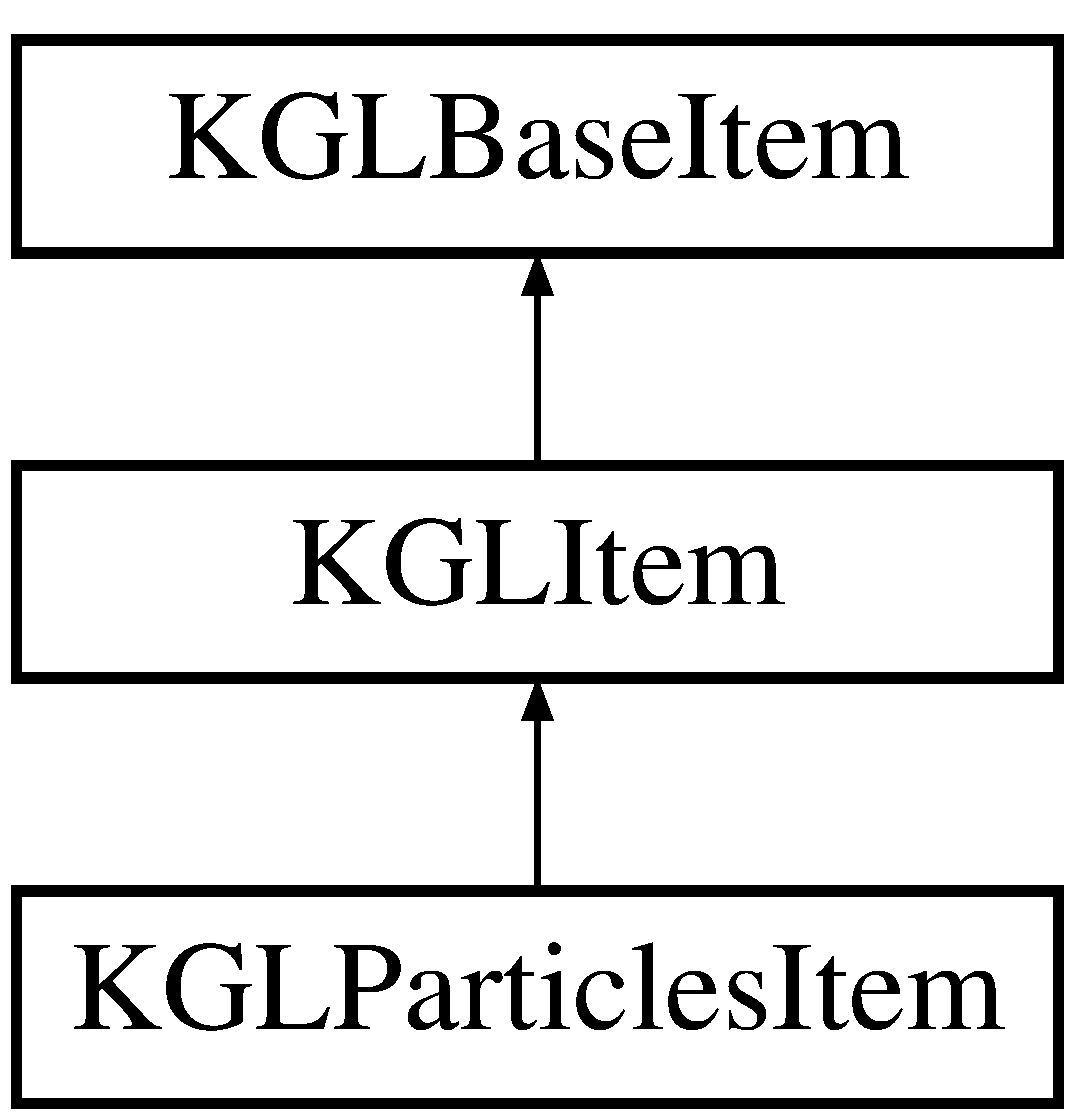
\includegraphics[height=3cm]{class_k_g_l_particles_item}
\end{center}
\end{figure}
\subsection*{Public Member Functions}
\begin{CompactItemize}
\item 
\hyperlink{class_k_g_l_particles_item_f9d2aff0b3f2f6b8b2e188cf7c69b99d}{KGLParticlesItem} (\hyperlink{class_k_g_l_engine}{KGLEngine} $\ast$parent=0)
\item 
virtual void \hyperlink{class_k_g_l_particles_item_ce6df2f63f0566993f075f7ce55bb714}{draw} ()
\item 
void \hyperlink{class_k_g_l_particles_item_e9b4281df0cdce181e5c72674d3b62fd}{addParticles} (\hyperlink{class_k_g_l_particle}{KGLParticle} $\ast$p)
\item 
QList$<$ \hyperlink{class_k_g_l_particle}{KGLParticle} $\ast$ $>$ \hyperlink{class_k_g_l_particles_item_fd39ca4535f227749edc932acbfb23f9}{particles} ()
\item 
void \hyperlink{class_k_g_l_particles_item_0d5e698526a16718ee51d33ef6c3c28d}{createExplose} (unsigned int number, QPixmap texture, const double angle=360, float speed=0.01, float alphaStep=0.01, float size=10)
\item 
void \hyperlink{class_k_g_l_particles_item_55ff83e136b35f0caaeb0ef065623573}{createSmoke} (unsigned int number, QPixmap texture, const double angle=360, float speed=0.01, float alphaStep=0.01, float size=10)
\end{CompactItemize}


\subsection{Constructor \& Destructor Documentation}
\hypertarget{class_k_g_l_particles_item_f9d2aff0b3f2f6b8b2e188cf7c69b99d}{
\index{KGLParticlesItem@{KGLParticlesItem}!KGLParticlesItem@{KGLParticlesItem}}
\index{KGLParticlesItem@{KGLParticlesItem}!KGLParticlesItem@{KGLParticlesItem}}
\subsubsection[{KGLParticlesItem}]{\setlength{\rightskip}{0pt plus 5cm}KGLParticlesItem::KGLParticlesItem ({\bf KGLEngine} $\ast$ {\em parent} = {\tt 0})}}
\label{class_k_g_l_particles_item_f9d2aff0b3f2f6b8b2e188cf7c69b99d}




\subsection{Member Function Documentation}
\hypertarget{class_k_g_l_particles_item_e9b4281df0cdce181e5c72674d3b62fd}{
\index{KGLParticlesItem@{KGLParticlesItem}!addParticles@{addParticles}}
\index{addParticles@{addParticles}!KGLParticlesItem@{KGLParticlesItem}}
\subsubsection[{addParticles}]{\setlength{\rightskip}{0pt plus 5cm}void KGLParticlesItem::addParticles ({\bf KGLParticle} $\ast$ {\em p})\hspace{0.3cm}{\tt  \mbox{[}inline\mbox{]}}}}
\label{class_k_g_l_particles_item_e9b4281df0cdce181e5c72674d3b62fd}


\hypertarget{class_k_g_l_particles_item_0d5e698526a16718ee51d33ef6c3c28d}{
\index{KGLParticlesItem@{KGLParticlesItem}!createExplose@{createExplose}}
\index{createExplose@{createExplose}!KGLParticlesItem@{KGLParticlesItem}}
\subsubsection[{createExplose}]{\setlength{\rightskip}{0pt plus 5cm}void KGLParticlesItem::createExplose (unsigned int {\em number}, \/  QPixmap {\em texture}, \/  const double {\em angle} = {\tt 360}, \/  float {\em speed} = {\tt 0.01}, \/  float {\em alphaStep} = {\tt 0.01}, \/  float {\em size} = {\tt 10})}}
\label{class_k_g_l_particles_item_0d5e698526a16718ee51d33ef6c3c28d}


\hypertarget{class_k_g_l_particles_item_55ff83e136b35f0caaeb0ef065623573}{
\index{KGLParticlesItem@{KGLParticlesItem}!createSmoke@{createSmoke}}
\index{createSmoke@{createSmoke}!KGLParticlesItem@{KGLParticlesItem}}
\subsubsection[{createSmoke}]{\setlength{\rightskip}{0pt plus 5cm}void KGLParticlesItem::createSmoke (unsigned int {\em number}, \/  QPixmap {\em texture}, \/  const double {\em angle} = {\tt 360}, \/  float {\em speed} = {\tt 0.01}, \/  float {\em alphaStep} = {\tt 0.01}, \/  float {\em size} = {\tt 10})}}
\label{class_k_g_l_particles_item_55ff83e136b35f0caaeb0ef065623573}


\hypertarget{class_k_g_l_particles_item_ce6df2f63f0566993f075f7ce55bb714}{
\index{KGLParticlesItem@{KGLParticlesItem}!draw@{draw}}
\index{draw@{draw}!KGLParticlesItem@{KGLParticlesItem}}
\subsubsection[{draw}]{\setlength{\rightskip}{0pt plus 5cm}void KGLParticlesItem::draw ()\hspace{0.3cm}{\tt  \mbox{[}virtual\mbox{]}}}}
\label{class_k_g_l_particles_item_ce6df2f63f0566993f075f7ce55bb714}




Reimplemented from \hyperlink{class_k_g_l_item_4e4766cf0362fa050bffdf5f45d6d13f}{KGLItem}.\hypertarget{class_k_g_l_particles_item_fd39ca4535f227749edc932acbfb23f9}{
\index{KGLParticlesItem@{KGLParticlesItem}!particles@{particles}}
\index{particles@{particles}!KGLParticlesItem@{KGLParticlesItem}}
\subsubsection[{particles}]{\setlength{\rightskip}{0pt plus 5cm}QList$<${\bf KGLParticle}$\ast$$>$ KGLParticlesItem::particles ()\hspace{0.3cm}{\tt  \mbox{[}inline\mbox{]}}}}
\label{class_k_g_l_particles_item_fd39ca4535f227749edc932acbfb23f9}




The documentation for this class was generated from the following files:\begin{CompactItemize}
\item 
/home/sacha/programmation/gluon/kgl/\hyperlink{kglparticlesitem_8h}{kglparticlesitem.h}\item 
/home/sacha/programmation/gluon/kgl/\hyperlink{kglparticlesitem_8cpp}{kglparticlesitem.cpp}\end{CompactItemize}

\hypertarget{class_k_g_l_physics_engine}{
\section{KGLPhysicsEngine Class Reference}
\label{class_k_g_l_physics_engine}\index{KGLPhysicsEngine@{KGLPhysicsEngine}}
}
{\tt \#include $<$kglphysicsengine.h$>$}

Inheritance diagram for KGLPhysicsEngine::\begin{figure}[H]
\begin{center}
\leavevmode
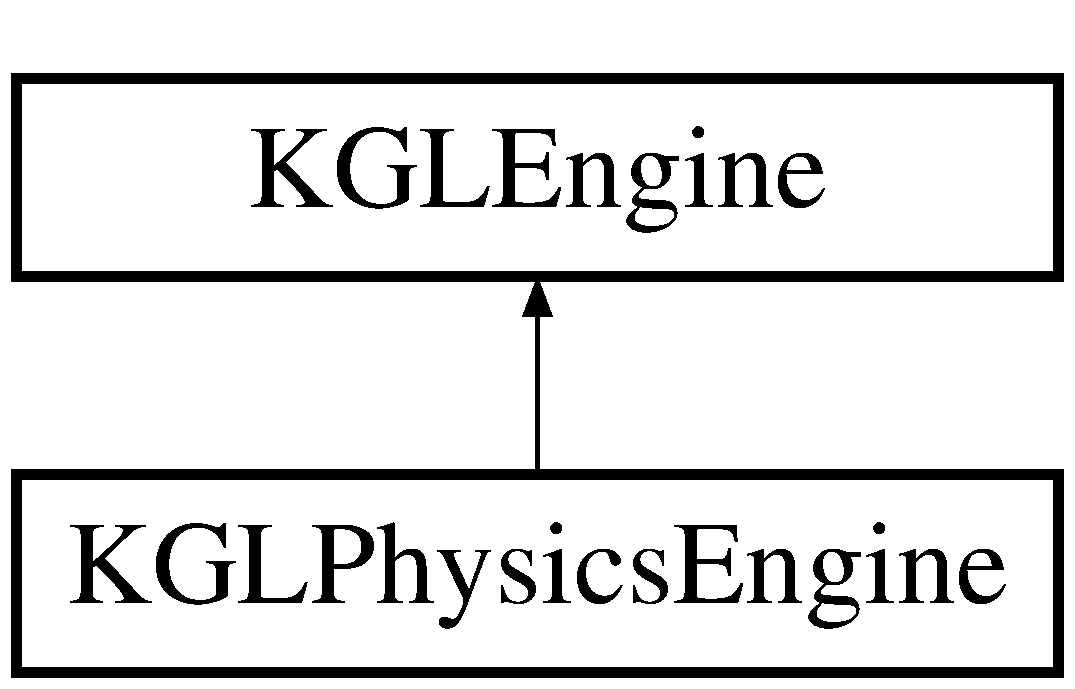
\includegraphics[height=2cm]{class_k_g_l_physics_engine}
\end{center}
\end{figure}
\subsection*{Public Slots}
\begin{CompactItemize}
\item 
void \hyperlink{class_k_g_l_physics_engine_6ec2dab4d2361f4904c7ca538efbe292}{clearPhysicsItem} ()
\item 
b2World $\ast$ \hyperlink{class_k_g_l_physics_engine_099fcf17ad1ecb1400e794c56705966a}{world} ()
\end{CompactItemize}
\subsection*{Public Member Functions}
\begin{CompactItemize}
\item 
\hyperlink{class_k_g_l_physics_engine_0818ba02342badbfbe03053d39b90039}{KGLPhysicsEngine} (QObject $\ast$parent=0)
\item 
\hyperlink{class_k_g_l_physics_engine_98c83543996d5546657cd66dc9f4e4c5}{$\sim$KGLPhysicsEngine} ()
\item 
virtual void \hyperlink{class_k_g_l_physics_engine_b72358d3b45888792d7c4e91715d29b4}{mainLoop} (float fps)
\item 
void \hyperlink{class_k_g_l_physics_engine_009c7c03e8f732078a884c6470fee7aa}{createWorld} ()
\item 
void \hyperlink{class_k_g_l_physics_engine_c93209f7f6e2fd36e088f1d27fb11c96}{computeSimulation} (int32 iterations=10, float fps=60)
\item 
void \hyperlink{class_k_g_l_physics_engine_94a77a670eb52594fa7aa468c3ef9fea}{addItem} (\hyperlink{class_k_g_l_physics_item}{KGLPhysicsItem} $\ast$item)
\item 
void \hyperlink{class_k_g_l_physics_engine_eefe31c558a83c43d1840987cdea1898}{addItem} (\hyperlink{class_k_g_l_item}{KGLItem} $\ast$item)
\item 
bool \hyperlink{class_k_g_l_physics_engine_86b45678b02feaab807db096a260063a}{removeItem} (\hyperlink{class_k_g_l_physics_item}{KGLPhysicsItem} $\ast$item)
\item 
bool \hyperlink{class_k_g_l_physics_engine_c5e88c0ab7ec1923038fdcb36ffdb192}{removeItem} (\hyperlink{class_k_g_l_item}{KGLItem} $\ast$item)
\item 
\hyperlink{class_k_g_l_physics_item}{KGLPhysicsItem} $\ast$ \hyperlink{class_k_g_l_physics_engine_7ee68f8b014f5523f4ab1e9959ea2993}{physicsItemAt} (QPointF pos)
\item 
QList$<$ \hyperlink{class_k_g_l_physics_item}{KGLPhysicsItem} $\ast$ $>$ \hyperlink{class_k_g_l_physics_engine_1024a6769903dc99982546d54fdd4a5e}{physicsItemList} ()
\item 
\hyperlink{class_k_g_l_physics_item}{KGLPhysicsItem} $\ast$ \hyperlink{class_k_g_l_physics_engine_93baa2d72eb792cf7139507186a3d0c4}{itemAt} (QPointF pos)
\item 
void \hyperlink{class_k_g_l_physics_engine_ada02faca27bd54213c1c73af61d0795}{setGravity} (const QPointF \&g)
\end{CompactItemize}


\subsection{Constructor \& Destructor Documentation}
\hypertarget{class_k_g_l_physics_engine_0818ba02342badbfbe03053d39b90039}{
\index{KGLPhysicsEngine@{KGLPhysicsEngine}!KGLPhysicsEngine@{KGLPhysicsEngine}}
\index{KGLPhysicsEngine@{KGLPhysicsEngine}!KGLPhysicsEngine@{KGLPhysicsEngine}}
\subsubsection[{KGLPhysicsEngine}]{\setlength{\rightskip}{0pt plus 5cm}KGLPhysicsEngine::KGLPhysicsEngine (QObject $\ast$ {\em parent} = {\tt 0})}}
\label{class_k_g_l_physics_engine_0818ba02342badbfbe03053d39b90039}


\hypertarget{class_k_g_l_physics_engine_98c83543996d5546657cd66dc9f4e4c5}{
\index{KGLPhysicsEngine@{KGLPhysicsEngine}!$\sim$KGLPhysicsEngine@{$\sim$KGLPhysicsEngine}}
\index{$\sim$KGLPhysicsEngine@{$\sim$KGLPhysicsEngine}!KGLPhysicsEngine@{KGLPhysicsEngine}}
\subsubsection[{$\sim$KGLPhysicsEngine}]{\setlength{\rightskip}{0pt plus 5cm}KGLPhysicsEngine::$\sim$KGLPhysicsEngine ()}}
\label{class_k_g_l_physics_engine_98c83543996d5546657cd66dc9f4e4c5}




\subsection{Member Function Documentation}
\hypertarget{class_k_g_l_physics_engine_eefe31c558a83c43d1840987cdea1898}{
\index{KGLPhysicsEngine@{KGLPhysicsEngine}!addItem@{addItem}}
\index{addItem@{addItem}!KGLPhysicsEngine@{KGLPhysicsEngine}}
\subsubsection[{addItem}]{\setlength{\rightskip}{0pt plus 5cm}void KGLPhysicsEngine::addItem ({\bf KGLItem} $\ast$ {\em item})\hspace{0.3cm}{\tt  \mbox{[}inline\mbox{]}}}}
\label{class_k_g_l_physics_engine_eefe31c558a83c43d1840987cdea1898}




Reimplemented from \hyperlink{class_k_g_l_engine_4aa9d5809d76cc44994a1cdb9df6f3ec}{KGLEngine}.\hypertarget{class_k_g_l_physics_engine_94a77a670eb52594fa7aa468c3ef9fea}{
\index{KGLPhysicsEngine@{KGLPhysicsEngine}!addItem@{addItem}}
\index{addItem@{addItem}!KGLPhysicsEngine@{KGLPhysicsEngine}}
\subsubsection[{addItem}]{\setlength{\rightskip}{0pt plus 5cm}void KGLPhysicsEngine::addItem ({\bf KGLPhysicsItem} $\ast$ {\em item})}}
\label{class_k_g_l_physics_engine_94a77a670eb52594fa7aa468c3ef9fea}


\hypertarget{class_k_g_l_physics_engine_6ec2dab4d2361f4904c7ca538efbe292}{
\index{KGLPhysicsEngine@{KGLPhysicsEngine}!clearPhysicsItem@{clearPhysicsItem}}
\index{clearPhysicsItem@{clearPhysicsItem}!KGLPhysicsEngine@{KGLPhysicsEngine}}
\subsubsection[{clearPhysicsItem}]{\setlength{\rightskip}{0pt plus 5cm}void KGLPhysicsEngine::clearPhysicsItem ()\hspace{0.3cm}{\tt  \mbox{[}slot\mbox{]}}}}
\label{class_k_g_l_physics_engine_6ec2dab4d2361f4904c7ca538efbe292}


\hypertarget{class_k_g_l_physics_engine_c93209f7f6e2fd36e088f1d27fb11c96}{
\index{KGLPhysicsEngine@{KGLPhysicsEngine}!computeSimulation@{computeSimulation}}
\index{computeSimulation@{computeSimulation}!KGLPhysicsEngine@{KGLPhysicsEngine}}
\subsubsection[{computeSimulation}]{\setlength{\rightskip}{0pt plus 5cm}void KGLPhysicsEngine::computeSimulation (int32 {\em iterations} = {\tt 10}, \/  float {\em fps} = {\tt 60})}}
\label{class_k_g_l_physics_engine_c93209f7f6e2fd36e088f1d27fb11c96}


\hypertarget{class_k_g_l_physics_engine_009c7c03e8f732078a884c6470fee7aa}{
\index{KGLPhysicsEngine@{KGLPhysicsEngine}!createWorld@{createWorld}}
\index{createWorld@{createWorld}!KGLPhysicsEngine@{KGLPhysicsEngine}}
\subsubsection[{createWorld}]{\setlength{\rightskip}{0pt plus 5cm}void KGLPhysicsEngine::createWorld ()}}
\label{class_k_g_l_physics_engine_009c7c03e8f732078a884c6470fee7aa}


\hypertarget{class_k_g_l_physics_engine_93baa2d72eb792cf7139507186a3d0c4}{
\index{KGLPhysicsEngine@{KGLPhysicsEngine}!itemAt@{itemAt}}
\index{itemAt@{itemAt}!KGLPhysicsEngine@{KGLPhysicsEngine}}
\subsubsection[{itemAt}]{\setlength{\rightskip}{0pt plus 5cm}{\bf KGLPhysicsItem} $\ast$ KGLPhysicsEngine::itemAt (QPointF {\em pos})}}
\label{class_k_g_l_physics_engine_93baa2d72eb792cf7139507186a3d0c4}


\hypertarget{class_k_g_l_physics_engine_b72358d3b45888792d7c4e91715d29b4}{
\index{KGLPhysicsEngine@{KGLPhysicsEngine}!mainLoop@{mainLoop}}
\index{mainLoop@{mainLoop}!KGLPhysicsEngine@{KGLPhysicsEngine}}
\subsubsection[{mainLoop}]{\setlength{\rightskip}{0pt plus 5cm}void KGLPhysicsEngine::mainLoop (float {\em fps})\hspace{0.3cm}{\tt  \mbox{[}virtual\mbox{]}}}}
\label{class_k_g_l_physics_engine_b72358d3b45888792d7c4e91715d29b4}




Reimplemented from \hyperlink{class_k_g_l_engine_787e1d8dfb58a6d6973a1f62c83b3263}{KGLEngine}.\hypertarget{class_k_g_l_physics_engine_7ee68f8b014f5523f4ab1e9959ea2993}{
\index{KGLPhysicsEngine@{KGLPhysicsEngine}!physicsItemAt@{physicsItemAt}}
\index{physicsItemAt@{physicsItemAt}!KGLPhysicsEngine@{KGLPhysicsEngine}}
\subsubsection[{physicsItemAt}]{\setlength{\rightskip}{0pt plus 5cm}{\bf KGLPhysicsItem}$\ast$ KGLPhysicsEngine::physicsItemAt (QPointF {\em pos})}}
\label{class_k_g_l_physics_engine_7ee68f8b014f5523f4ab1e9959ea2993}


\hypertarget{class_k_g_l_physics_engine_1024a6769903dc99982546d54fdd4a5e}{
\index{KGLPhysicsEngine@{KGLPhysicsEngine}!physicsItemList@{physicsItemList}}
\index{physicsItemList@{physicsItemList}!KGLPhysicsEngine@{KGLPhysicsEngine}}
\subsubsection[{physicsItemList}]{\setlength{\rightskip}{0pt plus 5cm}QList$<${\bf KGLPhysicsItem}$\ast$$>$ KGLPhysicsEngine::physicsItemList ()\hspace{0.3cm}{\tt  \mbox{[}inline\mbox{]}}}}
\label{class_k_g_l_physics_engine_1024a6769903dc99982546d54fdd4a5e}


\hypertarget{class_k_g_l_physics_engine_c5e88c0ab7ec1923038fdcb36ffdb192}{
\index{KGLPhysicsEngine@{KGLPhysicsEngine}!removeItem@{removeItem}}
\index{removeItem@{removeItem}!KGLPhysicsEngine@{KGLPhysicsEngine}}
\subsubsection[{removeItem}]{\setlength{\rightskip}{0pt plus 5cm}bool KGLPhysicsEngine::removeItem ({\bf KGLItem} $\ast$ {\em item})\hspace{0.3cm}{\tt  \mbox{[}inline\mbox{]}}}}
\label{class_k_g_l_physics_engine_c5e88c0ab7ec1923038fdcb36ffdb192}




Reimplemented from \hyperlink{class_k_g_l_engine_533f3324f67dcda39192365e2eab40c3}{KGLEngine}.\hypertarget{class_k_g_l_physics_engine_86b45678b02feaab807db096a260063a}{
\index{KGLPhysicsEngine@{KGLPhysicsEngine}!removeItem@{removeItem}}
\index{removeItem@{removeItem}!KGLPhysicsEngine@{KGLPhysicsEngine}}
\subsubsection[{removeItem}]{\setlength{\rightskip}{0pt plus 5cm}bool KGLPhysicsEngine::removeItem ({\bf KGLPhysicsItem} $\ast$ {\em item})}}
\label{class_k_g_l_physics_engine_86b45678b02feaab807db096a260063a}


\hypertarget{class_k_g_l_physics_engine_ada02faca27bd54213c1c73af61d0795}{
\index{KGLPhysicsEngine@{KGLPhysicsEngine}!setGravity@{setGravity}}
\index{setGravity@{setGravity}!KGLPhysicsEngine@{KGLPhysicsEngine}}
\subsubsection[{setGravity}]{\setlength{\rightskip}{0pt plus 5cm}void KGLPhysicsEngine::setGravity (const QPointF \& {\em g})\hspace{0.3cm}{\tt  \mbox{[}inline\mbox{]}}}}
\label{class_k_g_l_physics_engine_ada02faca27bd54213c1c73af61d0795}


\hypertarget{class_k_g_l_physics_engine_099fcf17ad1ecb1400e794c56705966a}{
\index{KGLPhysicsEngine@{KGLPhysicsEngine}!world@{world}}
\index{world@{world}!KGLPhysicsEngine@{KGLPhysicsEngine}}
\subsubsection[{world}]{\setlength{\rightskip}{0pt plus 5cm}b2World$\ast$ KGLPhysicsEngine::world ()\hspace{0.3cm}{\tt  \mbox{[}inline, slot\mbox{]}}}}
\label{class_k_g_l_physics_engine_099fcf17ad1ecb1400e794c56705966a}




The documentation for this class was generated from the following files:\begin{CompactItemize}
\item 
/home/sacha/programmation/gluon/kgl/\hyperlink{kglphysicsengine_8h}{kglphysicsengine.h}\item 
/home/sacha/programmation/gluon/kgl/\hyperlink{kglphysicsengine_8cpp}{kglphysicsengine.cpp}\end{CompactItemize}

\hypertarget{class_k_g_l_physics_item}{
\section{KGLPhysicsItem Class Reference}
\label{class_k_g_l_physics_item}\index{KGLPhysicsItem@{KGLPhysicsItem}}
}
{\tt \#include $<$kglphysicsitem.h$>$}

Inheritance diagram for KGLPhysicsItem::\begin{figure}[H]
\begin{center}
\leavevmode
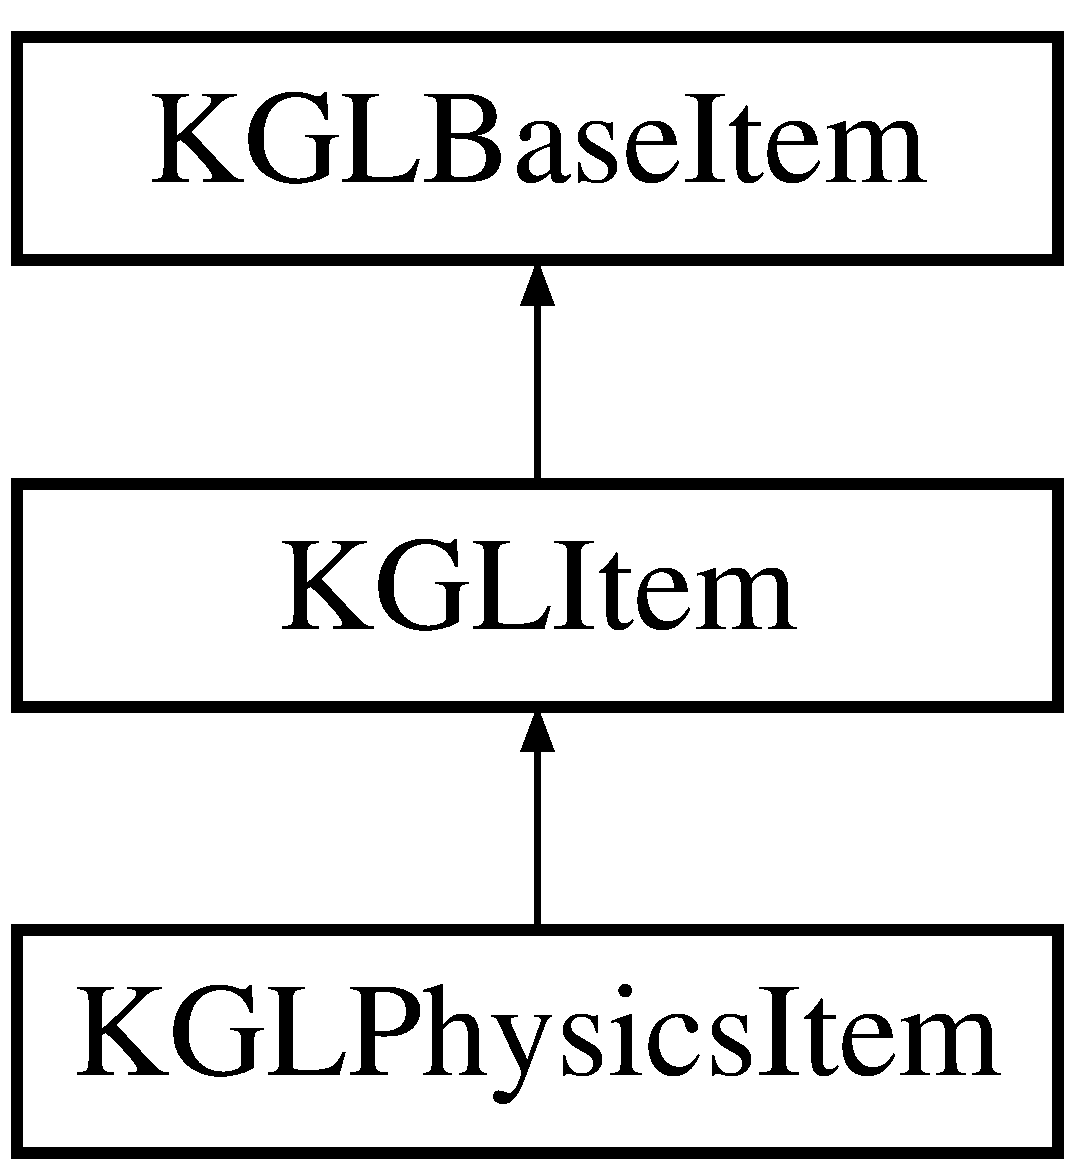
\includegraphics[height=3cm]{class_k_g_l_physics_item}
\end{center}
\end{figure}
\subsection*{Public Types}
\begin{CompactItemize}
\item 
enum \hyperlink{class_k_g_l_physics_item_b74dbd1e43d8bc18ec4fc6c16d3d4b7c}{SHAPE\_\-TYPE} \{ \hyperlink{class_k_g_l_physics_item_b74dbd1e43d8bc18ec4fc6c16d3d4b7c7f3449bf6512cac0a5dbf9aadc27b766}{POLYGON\_\-SHAPE} = 0, 
\hyperlink{class_k_g_l_physics_item_b74dbd1e43d8bc18ec4fc6c16d3d4b7c6b578fc66c478353e0e41ca78583a1e8}{CIRCLE\_\-SHAPE} = 1
 \}
\subsection*{Signals}
\begin{CompactItemize}
\item 
void \hyperlink{class_k_g_l_physics_item_839c757a057b738d58f315ea821a81a0}{collided} (\hyperlink{class_k_g_l_physics_item}{KGLPhysicsItem} $\ast$other)
\item 
void \hyperlink{class_k_g_l_physics_item_27a5f89aa48c78f0c3c18b20964eba24}{collided} ()
\end{CompactItemize}
\subsection*{Public Member Functions}
\begin{CompactItemize}
\item 
\hyperlink{class_k_g_l_physics_item_7930e195a22bd7e3b5809bd996cff4a4}{KGLPhysicsItem} (\hyperlink{class_k_g_l_engine}{KGLEngine} $\ast$parent=0)
\item 
void \hyperlink{class_k_g_l_physics_item_d1ec46b418f44e680e7726f2cab4aaf3}{setup} (b2World $\ast$world)
\item 
void \hyperlink{class_k_g_l_physics_item_bb70a21be98cab74c7daf10d6befbc09}{setupParam} ()
\item 
void \hyperlink{class_k_g_l_physics_item_fed8b6cdfbd684e5ed71f8af03bf9ab7}{updatePhysics} ()
\item 
b2Body $\ast$ \hyperlink{class_k_g_l_physics_item_1d2f1900e5bd95ac3699f42e8b8b9710}{body} ()
\item 
void \hyperlink{class_k_g_l_physics_item_a492016cac88405f5988d891c838c2d6}{setPolygonDef} (b2PolygonDef p)
\item 
void \hyperlink{class_k_g_l_physics_item_5596df9172f5ca0ea725419f0dce8db6}{setBodyDef} (b2BodyDef b)
\item 
void \hyperlink{class_k_g_l_physics_item_2a19b0749cfc745ad7ac0b6366185f41}{initDensity} (const float32 \&d)
\item 
void \hyperlink{class_k_g_l_physics_item_7523dc0a9453bd982a4f60d1734af46f}{initFriction} (const float32 \&f)
\item 
void \hyperlink{class_k_g_l_physics_item_6d8c120c3abedc0e6ba56905264c1d5b}{initRestitution} (const float32 \&r)
\item 
void \hyperlink{class_k_g_l_physics_item_bae743b4a3ac9f8db1b643438933a50b}{initSensor} (bool b)
\item 
void \hyperlink{class_k_g_l_physics_item_bf88ca0759ddebe73c41cdf42103f04f}{setMass} (const float32 \&m)
\item 
void \hyperlink{class_k_g_l_physics_item_8596bfa11f1267e39031d3a8b14d55e0}{initLinearDamping} (const float32 \&l)
\item 
void \hyperlink{class_k_g_l_physics_item_7041239eb6f4eaba7a921009d0fcdcf6}{initAngularDamping} (const float32 \&a)
\item 
void \hyperlink{class_k_g_l_physics_item_3b9673bad884214365837e3f87c35358}{initCategoryBits} (const uint16 \&c)
\item 
void \hyperlink{class_k_g_l_physics_item_0837f29f919d93cfca1429415b072b22}{initMaskBits} (const uint16 \&c)
\item 
void \hyperlink{class_k_g_l_physics_item_8ccd7feacbfc2c4e6d035bc147138cde}{setMassFromShape} (bool b)
\item 
void \hyperlink{class_k_g_l_physics_item_10f8810cfd4018543a169df37a7a7cc1}{setStatic} ()
\item 
void \hyperlink{class_k_g_l_physics_item_8c86227c571bfa83e6aefbaa1ef573df}{setShapeType} (\hyperlink{class_k_g_l_physics_item_b74dbd1e43d8bc18ec4fc6c16d3d4b7c}{SHAPE\_\-TYPE} t=POLYGON\_\-SHAPE)
\item 
b2PolygonDef $\ast$ \hyperlink{class_k_g_l_physics_item_ca68c4c36791432954708a3253ac1f73}{polygonDef} ()
\item 
b2BodyDef $\ast$ \hyperlink{class_k_g_l_physics_item_384af73ef980d7404c4e4cf4332bb332}{bodyDef} ()
\item 
const float32 \& \hyperlink{class_k_g_l_physics_item_c908866d9a749e6bce529b6e4f3ed80b}{density} ()
\item 
const float32 \& \hyperlink{class_k_g_l_physics_item_656cc790aa2b53f3c45e4488aad35887}{friction} ()
\item 
const float32 \& \hyperlink{class_k_g_l_physics_item_a6fec0352a3214ab5ec031eccc2952ac}{restition} ()
\item 
const float32 \& \hyperlink{class_k_g_l_physics_item_17c7c15ab2ec62db4f17da9cc31506da}{mass} ()
\item 
bool \hyperlink{class_k_g_l_physics_item_eddb441690ec42d679aba642bc12dee3}{isSensor} ()
\item 
const float32 \& \hyperlink{class_k_g_l_physics_item_e83c6834e417cd7da10481d0878b9c40}{linearDamping} ()
\item 
const float32 \& \hyperlink{class_k_g_l_physics_item_faf0f2e3fd56195ce1e165b5f206855a}{angularDamping} ()
\item 
const uint16 \& \hyperlink{class_k_g_l_physics_item_870ea0d4451995acf418807dd535d82d}{categoryBits} ()
\item 
const uint16 \& \hyperlink{class_k_g_l_physics_item_4d60872591ae5b15ebd01f2f46c40ab6}{maskBits} ()
\item 
virtual void \hyperlink{class_k_g_l_physics_item_e531b03571d9d7bc17a76bbf9fbc2d8a}{collidesWithItem} (\hyperlink{class_k_g_l_physics_item}{KGLPhysicsItem} $\ast$other)
\end{CompactItemize}


\subsection{Member Enumeration Documentation}
\hypertarget{class_k_g_l_physics_item_b74dbd1e43d8bc18ec4fc6c16d3d4b7c}{
\index{KGLPhysicsItem@{KGLPhysicsItem}!SHAPE\_\-TYPE@{SHAPE\_\-TYPE}}
\index{SHAPE\_\-TYPE@{SHAPE\_\-TYPE}!KGLPhysicsItem@{KGLPhysicsItem}}
\subsubsection[{SHAPE\_\-TYPE}]{\setlength{\rightskip}{0pt plus 5cm}enum {\bf KGLPhysicsItem::SHAPE\_\-TYPE}}}
\label{class_k_g_l_physics_item_b74dbd1e43d8bc18ec4fc6c16d3d4b7c}


\begin{Desc}
\item[Enumerator: ]\par
\begin{description}
\index{POLYGON\_\-SHAPE@{POLYGON\_\-SHAPE}!KGLPhysicsItem@{KGLPhysicsItem}}\index{KGLPhysicsItem@{KGLPhysicsItem}!POLYGON\_\-SHAPE@{POLYGON\_\-SHAPE}}\item[{\em 
\hypertarget{class_k_g_l_physics_item_b74dbd1e43d8bc18ec4fc6c16d3d4b7c7f3449bf6512cac0a5dbf9aadc27b766}{
POLYGON\_\-SHAPE}
\label{class_k_g_l_physics_item_b74dbd1e43d8bc18ec4fc6c16d3d4b7c7f3449bf6512cac0a5dbf9aadc27b766}
}]\index{CIRCLE\_\-SHAPE@{CIRCLE\_\-SHAPE}!KGLPhysicsItem@{KGLPhysicsItem}}\index{KGLPhysicsItem@{KGLPhysicsItem}!CIRCLE\_\-SHAPE@{CIRCLE\_\-SHAPE}}\item[{\em 
\hypertarget{class_k_g_l_physics_item_b74dbd1e43d8bc18ec4fc6c16d3d4b7c6b578fc66c478353e0e41ca78583a1e8}{
CIRCLE\_\-SHAPE}
\label{class_k_g_l_physics_item_b74dbd1e43d8bc18ec4fc6c16d3d4b7c6b578fc66c478353e0e41ca78583a1e8}
}]\end{description}
\end{Desc}



\subsection{Constructor \& Destructor Documentation}
\hypertarget{class_k_g_l_physics_item_7930e195a22bd7e3b5809bd996cff4a4}{
\index{KGLPhysicsItem@{KGLPhysicsItem}!KGLPhysicsItem@{KGLPhysicsItem}}
\index{KGLPhysicsItem@{KGLPhysicsItem}!KGLPhysicsItem@{KGLPhysicsItem}}
\subsubsection[{KGLPhysicsItem}]{\setlength{\rightskip}{0pt plus 5cm}KGLPhysicsItem::KGLPhysicsItem ({\bf KGLEngine} $\ast$ {\em parent} = {\tt 0})}}
\label{class_k_g_l_physics_item_7930e195a22bd7e3b5809bd996cff4a4}




\subsection{Member Function Documentation}
\hypertarget{class_k_g_l_physics_item_faf0f2e3fd56195ce1e165b5f206855a}{
\index{KGLPhysicsItem@{KGLPhysicsItem}!angularDamping@{angularDamping}}
\index{angularDamping@{angularDamping}!KGLPhysicsItem@{KGLPhysicsItem}}
\subsubsection[{angularDamping}]{\setlength{\rightskip}{0pt plus 5cm}const float32\& KGLPhysicsItem::angularDamping ()\hspace{0.3cm}{\tt  \mbox{[}inline\mbox{]}}}}
\label{class_k_g_l_physics_item_faf0f2e3fd56195ce1e165b5f206855a}


\hypertarget{class_k_g_l_physics_item_1d2f1900e5bd95ac3699f42e8b8b9710}{
\index{KGLPhysicsItem@{KGLPhysicsItem}!body@{body}}
\index{body@{body}!KGLPhysicsItem@{KGLPhysicsItem}}
\subsubsection[{body}]{\setlength{\rightskip}{0pt plus 5cm}b2Body $\ast$ KGLPhysicsItem::body ()}}
\label{class_k_g_l_physics_item_1d2f1900e5bd95ac3699f42e8b8b9710}


\hypertarget{class_k_g_l_physics_item_384af73ef980d7404c4e4cf4332bb332}{
\index{KGLPhysicsItem@{KGLPhysicsItem}!bodyDef@{bodyDef}}
\index{bodyDef@{bodyDef}!KGLPhysicsItem@{KGLPhysicsItem}}
\subsubsection[{bodyDef}]{\setlength{\rightskip}{0pt plus 5cm}b2BodyDef$\ast$ KGLPhysicsItem::bodyDef ()\hspace{0.3cm}{\tt  \mbox{[}inline\mbox{]}}}}
\label{class_k_g_l_physics_item_384af73ef980d7404c4e4cf4332bb332}


\hypertarget{class_k_g_l_physics_item_870ea0d4451995acf418807dd535d82d}{
\index{KGLPhysicsItem@{KGLPhysicsItem}!categoryBits@{categoryBits}}
\index{categoryBits@{categoryBits}!KGLPhysicsItem@{KGLPhysicsItem}}
\subsubsection[{categoryBits}]{\setlength{\rightskip}{0pt plus 5cm}const uint16\& KGLPhysicsItem::categoryBits ()\hspace{0.3cm}{\tt  \mbox{[}inline\mbox{]}}}}
\label{class_k_g_l_physics_item_870ea0d4451995acf418807dd535d82d}


\hypertarget{class_k_g_l_physics_item_27a5f89aa48c78f0c3c18b20964eba24}{
\index{KGLPhysicsItem@{KGLPhysicsItem}!collided@{collided}}
\index{collided@{collided}!KGLPhysicsItem@{KGLPhysicsItem}}
\subsubsection[{collided}]{\setlength{\rightskip}{0pt plus 5cm}void KGLPhysicsItem::collided ()\hspace{0.3cm}{\tt  \mbox{[}signal\mbox{]}}}}
\label{class_k_g_l_physics_item_27a5f89aa48c78f0c3c18b20964eba24}


\hypertarget{class_k_g_l_physics_item_839c757a057b738d58f315ea821a81a0}{
\index{KGLPhysicsItem@{KGLPhysicsItem}!collided@{collided}}
\index{collided@{collided}!KGLPhysicsItem@{KGLPhysicsItem}}
\subsubsection[{collided}]{\setlength{\rightskip}{0pt plus 5cm}void KGLPhysicsItem::collided ({\bf KGLPhysicsItem} $\ast$ {\em other})\hspace{0.3cm}{\tt  \mbox{[}signal\mbox{]}}}}
\label{class_k_g_l_physics_item_839c757a057b738d58f315ea821a81a0}


\hypertarget{class_k_g_l_physics_item_e531b03571d9d7bc17a76bbf9fbc2d8a}{
\index{KGLPhysicsItem@{KGLPhysicsItem}!collidesWithItem@{collidesWithItem}}
\index{collidesWithItem@{collidesWithItem}!KGLPhysicsItem@{KGLPhysicsItem}}
\subsubsection[{collidesWithItem}]{\setlength{\rightskip}{0pt plus 5cm}virtual void KGLPhysicsItem::collidesWithItem ({\bf KGLPhysicsItem} $\ast$ {\em other})\hspace{0.3cm}{\tt  \mbox{[}inline, virtual\mbox{]}}}}
\label{class_k_g_l_physics_item_e531b03571d9d7bc17a76bbf9fbc2d8a}


\hypertarget{class_k_g_l_physics_item_c908866d9a749e6bce529b6e4f3ed80b}{
\index{KGLPhysicsItem@{KGLPhysicsItem}!density@{density}}
\index{density@{density}!KGLPhysicsItem@{KGLPhysicsItem}}
\subsubsection[{density}]{\setlength{\rightskip}{0pt plus 5cm}const float32\& KGLPhysicsItem::density ()\hspace{0.3cm}{\tt  \mbox{[}inline\mbox{]}}}}
\label{class_k_g_l_physics_item_c908866d9a749e6bce529b6e4f3ed80b}


\hypertarget{class_k_g_l_physics_item_656cc790aa2b53f3c45e4488aad35887}{
\index{KGLPhysicsItem@{KGLPhysicsItem}!friction@{friction}}
\index{friction@{friction}!KGLPhysicsItem@{KGLPhysicsItem}}
\subsubsection[{friction}]{\setlength{\rightskip}{0pt plus 5cm}const float32\& KGLPhysicsItem::friction ()\hspace{0.3cm}{\tt  \mbox{[}inline\mbox{]}}}}
\label{class_k_g_l_physics_item_656cc790aa2b53f3c45e4488aad35887}


\hypertarget{class_k_g_l_physics_item_7041239eb6f4eaba7a921009d0fcdcf6}{
\index{KGLPhysicsItem@{KGLPhysicsItem}!initAngularDamping@{initAngularDamping}}
\index{initAngularDamping@{initAngularDamping}!KGLPhysicsItem@{KGLPhysicsItem}}
\subsubsection[{initAngularDamping}]{\setlength{\rightskip}{0pt plus 5cm}void KGLPhysicsItem::initAngularDamping (const float32 \& {\em a})\hspace{0.3cm}{\tt  \mbox{[}inline\mbox{]}}}}
\label{class_k_g_l_physics_item_7041239eb6f4eaba7a921009d0fcdcf6}


\hypertarget{class_k_g_l_physics_item_3b9673bad884214365837e3f87c35358}{
\index{KGLPhysicsItem@{KGLPhysicsItem}!initCategoryBits@{initCategoryBits}}
\index{initCategoryBits@{initCategoryBits}!KGLPhysicsItem@{KGLPhysicsItem}}
\subsubsection[{initCategoryBits}]{\setlength{\rightskip}{0pt plus 5cm}void KGLPhysicsItem::initCategoryBits (const uint16 \& {\em c})\hspace{0.3cm}{\tt  \mbox{[}inline\mbox{]}}}}
\label{class_k_g_l_physics_item_3b9673bad884214365837e3f87c35358}


\hypertarget{class_k_g_l_physics_item_2a19b0749cfc745ad7ac0b6366185f41}{
\index{KGLPhysicsItem@{KGLPhysicsItem}!initDensity@{initDensity}}
\index{initDensity@{initDensity}!KGLPhysicsItem@{KGLPhysicsItem}}
\subsubsection[{initDensity}]{\setlength{\rightskip}{0pt plus 5cm}void KGLPhysicsItem::initDensity (const float32 \& {\em d})\hspace{0.3cm}{\tt  \mbox{[}inline\mbox{]}}}}
\label{class_k_g_l_physics_item_2a19b0749cfc745ad7ac0b6366185f41}


\hypertarget{class_k_g_l_physics_item_7523dc0a9453bd982a4f60d1734af46f}{
\index{KGLPhysicsItem@{KGLPhysicsItem}!initFriction@{initFriction}}
\index{initFriction@{initFriction}!KGLPhysicsItem@{KGLPhysicsItem}}
\subsubsection[{initFriction}]{\setlength{\rightskip}{0pt plus 5cm}void KGLPhysicsItem::initFriction (const float32 \& {\em f})\hspace{0.3cm}{\tt  \mbox{[}inline\mbox{]}}}}
\label{class_k_g_l_physics_item_7523dc0a9453bd982a4f60d1734af46f}


\hypertarget{class_k_g_l_physics_item_8596bfa11f1267e39031d3a8b14d55e0}{
\index{KGLPhysicsItem@{KGLPhysicsItem}!initLinearDamping@{initLinearDamping}}
\index{initLinearDamping@{initLinearDamping}!KGLPhysicsItem@{KGLPhysicsItem}}
\subsubsection[{initLinearDamping}]{\setlength{\rightskip}{0pt plus 5cm}void KGLPhysicsItem::initLinearDamping (const float32 \& {\em l})\hspace{0.3cm}{\tt  \mbox{[}inline\mbox{]}}}}
\label{class_k_g_l_physics_item_8596bfa11f1267e39031d3a8b14d55e0}


\hypertarget{class_k_g_l_physics_item_0837f29f919d93cfca1429415b072b22}{
\index{KGLPhysicsItem@{KGLPhysicsItem}!initMaskBits@{initMaskBits}}
\index{initMaskBits@{initMaskBits}!KGLPhysicsItem@{KGLPhysicsItem}}
\subsubsection[{initMaskBits}]{\setlength{\rightskip}{0pt plus 5cm}void KGLPhysicsItem::initMaskBits (const uint16 \& {\em c})\hspace{0.3cm}{\tt  \mbox{[}inline\mbox{]}}}}
\label{class_k_g_l_physics_item_0837f29f919d93cfca1429415b072b22}


\hypertarget{class_k_g_l_physics_item_6d8c120c3abedc0e6ba56905264c1d5b}{
\index{KGLPhysicsItem@{KGLPhysicsItem}!initRestitution@{initRestitution}}
\index{initRestitution@{initRestitution}!KGLPhysicsItem@{KGLPhysicsItem}}
\subsubsection[{initRestitution}]{\setlength{\rightskip}{0pt plus 5cm}void KGLPhysicsItem::initRestitution (const float32 \& {\em r})\hspace{0.3cm}{\tt  \mbox{[}inline\mbox{]}}}}
\label{class_k_g_l_physics_item_6d8c120c3abedc0e6ba56905264c1d5b}


\hypertarget{class_k_g_l_physics_item_bae743b4a3ac9f8db1b643438933a50b}{
\index{KGLPhysicsItem@{KGLPhysicsItem}!initSensor@{initSensor}}
\index{initSensor@{initSensor}!KGLPhysicsItem@{KGLPhysicsItem}}
\subsubsection[{initSensor}]{\setlength{\rightskip}{0pt plus 5cm}void KGLPhysicsItem::initSensor (bool {\em b})\hspace{0.3cm}{\tt  \mbox{[}inline\mbox{]}}}}
\label{class_k_g_l_physics_item_bae743b4a3ac9f8db1b643438933a50b}


\hypertarget{class_k_g_l_physics_item_eddb441690ec42d679aba642bc12dee3}{
\index{KGLPhysicsItem@{KGLPhysicsItem}!isSensor@{isSensor}}
\index{isSensor@{isSensor}!KGLPhysicsItem@{KGLPhysicsItem}}
\subsubsection[{isSensor}]{\setlength{\rightskip}{0pt plus 5cm}bool KGLPhysicsItem::isSensor ()\hspace{0.3cm}{\tt  \mbox{[}inline\mbox{]}}}}
\label{class_k_g_l_physics_item_eddb441690ec42d679aba642bc12dee3}


\hypertarget{class_k_g_l_physics_item_e83c6834e417cd7da10481d0878b9c40}{
\index{KGLPhysicsItem@{KGLPhysicsItem}!linearDamping@{linearDamping}}
\index{linearDamping@{linearDamping}!KGLPhysicsItem@{KGLPhysicsItem}}
\subsubsection[{linearDamping}]{\setlength{\rightskip}{0pt plus 5cm}const float32\& KGLPhysicsItem::linearDamping ()\hspace{0.3cm}{\tt  \mbox{[}inline\mbox{]}}}}
\label{class_k_g_l_physics_item_e83c6834e417cd7da10481d0878b9c40}


\hypertarget{class_k_g_l_physics_item_4d60872591ae5b15ebd01f2f46c40ab6}{
\index{KGLPhysicsItem@{KGLPhysicsItem}!maskBits@{maskBits}}
\index{maskBits@{maskBits}!KGLPhysicsItem@{KGLPhysicsItem}}
\subsubsection[{maskBits}]{\setlength{\rightskip}{0pt plus 5cm}const uint16\& KGLPhysicsItem::maskBits ()\hspace{0.3cm}{\tt  \mbox{[}inline\mbox{]}}}}
\label{class_k_g_l_physics_item_4d60872591ae5b15ebd01f2f46c40ab6}


\hypertarget{class_k_g_l_physics_item_17c7c15ab2ec62db4f17da9cc31506da}{
\index{KGLPhysicsItem@{KGLPhysicsItem}!mass@{mass}}
\index{mass@{mass}!KGLPhysicsItem@{KGLPhysicsItem}}
\subsubsection[{mass}]{\setlength{\rightskip}{0pt plus 5cm}const float32\& KGLPhysicsItem::mass ()\hspace{0.3cm}{\tt  \mbox{[}inline\mbox{]}}}}
\label{class_k_g_l_physics_item_17c7c15ab2ec62db4f17da9cc31506da}


\hypertarget{class_k_g_l_physics_item_ca68c4c36791432954708a3253ac1f73}{
\index{KGLPhysicsItem@{KGLPhysicsItem}!polygonDef@{polygonDef}}
\index{polygonDef@{polygonDef}!KGLPhysicsItem@{KGLPhysicsItem}}
\subsubsection[{polygonDef}]{\setlength{\rightskip}{0pt plus 5cm}b2PolygonDef$\ast$ KGLPhysicsItem::polygonDef ()\hspace{0.3cm}{\tt  \mbox{[}inline\mbox{]}}}}
\label{class_k_g_l_physics_item_ca68c4c36791432954708a3253ac1f73}


\hypertarget{class_k_g_l_physics_item_a6fec0352a3214ab5ec031eccc2952ac}{
\index{KGLPhysicsItem@{KGLPhysicsItem}!restition@{restition}}
\index{restition@{restition}!KGLPhysicsItem@{KGLPhysicsItem}}
\subsubsection[{restition}]{\setlength{\rightskip}{0pt plus 5cm}const float32\& KGLPhysicsItem::restition ()\hspace{0.3cm}{\tt  \mbox{[}inline\mbox{]}}}}
\label{class_k_g_l_physics_item_a6fec0352a3214ab5ec031eccc2952ac}


\hypertarget{class_k_g_l_physics_item_5596df9172f5ca0ea725419f0dce8db6}{
\index{KGLPhysicsItem@{KGLPhysicsItem}!setBodyDef@{setBodyDef}}
\index{setBodyDef@{setBodyDef}!KGLPhysicsItem@{KGLPhysicsItem}}
\subsubsection[{setBodyDef}]{\setlength{\rightskip}{0pt plus 5cm}void KGLPhysicsItem::setBodyDef (b2BodyDef {\em b})\hspace{0.3cm}{\tt  \mbox{[}inline\mbox{]}}}}
\label{class_k_g_l_physics_item_5596df9172f5ca0ea725419f0dce8db6}


\hypertarget{class_k_g_l_physics_item_bf88ca0759ddebe73c41cdf42103f04f}{
\index{KGLPhysicsItem@{KGLPhysicsItem}!setMass@{setMass}}
\index{setMass@{setMass}!KGLPhysicsItem@{KGLPhysicsItem}}
\subsubsection[{setMass}]{\setlength{\rightskip}{0pt plus 5cm}void KGLPhysicsItem::setMass (const float32 \& {\em m})\hspace{0.3cm}{\tt  \mbox{[}inline\mbox{]}}}}
\label{class_k_g_l_physics_item_bf88ca0759ddebe73c41cdf42103f04f}


\hypertarget{class_k_g_l_physics_item_8ccd7feacbfc2c4e6d035bc147138cde}{
\index{KGLPhysicsItem@{KGLPhysicsItem}!setMassFromShape@{setMassFromShape}}
\index{setMassFromShape@{setMassFromShape}!KGLPhysicsItem@{KGLPhysicsItem}}
\subsubsection[{setMassFromShape}]{\setlength{\rightskip}{0pt plus 5cm}void KGLPhysicsItem::setMassFromShape (bool {\em b})\hspace{0.3cm}{\tt  \mbox{[}inline\mbox{]}}}}
\label{class_k_g_l_physics_item_8ccd7feacbfc2c4e6d035bc147138cde}


\hypertarget{class_k_g_l_physics_item_a492016cac88405f5988d891c838c2d6}{
\index{KGLPhysicsItem@{KGLPhysicsItem}!setPolygonDef@{setPolygonDef}}
\index{setPolygonDef@{setPolygonDef}!KGLPhysicsItem@{KGLPhysicsItem}}
\subsubsection[{setPolygonDef}]{\setlength{\rightskip}{0pt plus 5cm}void KGLPhysicsItem::setPolygonDef (b2PolygonDef {\em p})\hspace{0.3cm}{\tt  \mbox{[}inline\mbox{]}}}}
\label{class_k_g_l_physics_item_a492016cac88405f5988d891c838c2d6}


\hypertarget{class_k_g_l_physics_item_8c86227c571bfa83e6aefbaa1ef573df}{
\index{KGLPhysicsItem@{KGLPhysicsItem}!setShapeType@{setShapeType}}
\index{setShapeType@{setShapeType}!KGLPhysicsItem@{KGLPhysicsItem}}
\subsubsection[{setShapeType}]{\setlength{\rightskip}{0pt plus 5cm}void KGLPhysicsItem::setShapeType ({\bf SHAPE\_\-TYPE} {\em t} = {\tt POLYGON\_\-SHAPE})\hspace{0.3cm}{\tt  \mbox{[}inline\mbox{]}}}}
\label{class_k_g_l_physics_item_8c86227c571bfa83e6aefbaa1ef573df}


\hypertarget{class_k_g_l_physics_item_10f8810cfd4018543a169df37a7a7cc1}{
\index{KGLPhysicsItem@{KGLPhysicsItem}!setStatic@{setStatic}}
\index{setStatic@{setStatic}!KGLPhysicsItem@{KGLPhysicsItem}}
\subsubsection[{setStatic}]{\setlength{\rightskip}{0pt plus 5cm}void KGLPhysicsItem::setStatic ()\hspace{0.3cm}{\tt  \mbox{[}inline\mbox{]}}}}
\label{class_k_g_l_physics_item_10f8810cfd4018543a169df37a7a7cc1}


\hypertarget{class_k_g_l_physics_item_d1ec46b418f44e680e7726f2cab4aaf3}{
\index{KGLPhysicsItem@{KGLPhysicsItem}!setup@{setup}}
\index{setup@{setup}!KGLPhysicsItem@{KGLPhysicsItem}}
\subsubsection[{setup}]{\setlength{\rightskip}{0pt plus 5cm}void KGLPhysicsItem::setup (b2World $\ast$ {\em world})}}
\label{class_k_g_l_physics_item_d1ec46b418f44e680e7726f2cab4aaf3}


\hypertarget{class_k_g_l_physics_item_bb70a21be98cab74c7daf10d6befbc09}{
\index{KGLPhysicsItem@{KGLPhysicsItem}!setupParam@{setupParam}}
\index{setupParam@{setupParam}!KGLPhysicsItem@{KGLPhysicsItem}}
\subsubsection[{setupParam}]{\setlength{\rightskip}{0pt plus 5cm}void KGLPhysicsItem::setupParam ()}}
\label{class_k_g_l_physics_item_bb70a21be98cab74c7daf10d6befbc09}


\hypertarget{class_k_g_l_physics_item_fed8b6cdfbd684e5ed71f8af03bf9ab7}{
\index{KGLPhysicsItem@{KGLPhysicsItem}!updatePhysics@{updatePhysics}}
\index{updatePhysics@{updatePhysics}!KGLPhysicsItem@{KGLPhysicsItem}}
\subsubsection[{updatePhysics}]{\setlength{\rightskip}{0pt plus 5cm}void KGLPhysicsItem::updatePhysics ()}}
\label{class_k_g_l_physics_item_fed8b6cdfbd684e5ed71f8af03bf9ab7}




The documentation for this class was generated from the following files:\begin{CompactItemize}
\item 
/home/sacha/programmation/gluon/kgl/\hyperlink{kglphysicsitem_8h}{kglphysicsitem.h}\item 
/home/sacha/programmation/gluon/kgl/\hyperlink{kglphysicsitem_8cpp}{kglphysicsitem.cpp}\end{CompactItemize}

\hypertarget{class_k_g_l_pixelate_fx}{
\section{KGLPixelateFx Class Reference}
\label{class_k_g_l_pixelate_fx}\index{KGLPixelateFx@{KGLPixelateFx}}
}
{\tt \#include $<$kglfx.h$>$}

Inheritance diagram for KGLPixelateFx::\begin{figure}[H]
\begin{center}
\leavevmode
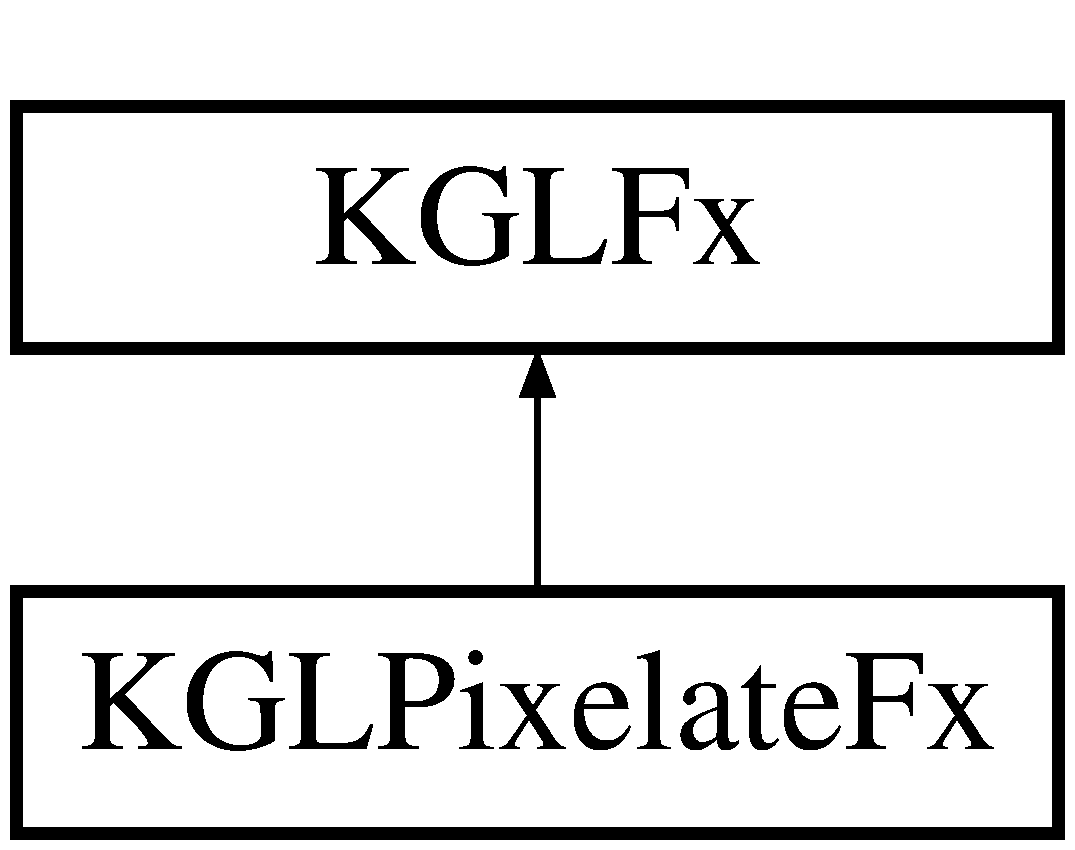
\includegraphics[height=2cm]{class_k_g_l_pixelate_fx}
\end{center}
\end{figure}
\subsection*{Public Member Functions}
\begin{CompactItemize}
\item 
\hyperlink{class_k_g_l_pixelate_fx_ed6f07a2e5ed5818d171e95f9ecac592}{KGLPixelateFx} ()
\item 
void \hyperlink{class_k_g_l_pixelate_fx_204ec29ca116f9fd7ba83b0d269529b6}{setAngle} (const float \&a)
\item 
void \hyperlink{class_k_g_l_pixelate_fx_fec0e778766d9ef081b3d676b90993f4}{setAngleMin} (const float \&a)
\item 
void \hyperlink{class_k_g_l_pixelate_fx_4f4806fa9000a7d9cb1b299107d4bdb2}{setAngleWidth} (const float \&a)
\item 
void \hyperlink{class_k_g_l_pixelate_fx_78842d2a1c034c8144688a07205b8c14}{setRadius} (const float \&r)
\item 
void \hyperlink{class_k_g_l_pixelate_fx_820ae55f76af24a334f80cd0d805f762}{setRadiusMin} (const float \&r)
\item 
void \hyperlink{class_k_g_l_pixelate_fx_b846b6766342b4bc502d73afad6b7094}{setRadiusWidth} (const float \&r)
\end{CompactItemize}


\subsection{Constructor \& Destructor Documentation}
\hypertarget{class_k_g_l_pixelate_fx_ed6f07a2e5ed5818d171e95f9ecac592}{
\index{KGLPixelateFx@{KGLPixelateFx}!KGLPixelateFx@{KGLPixelateFx}}
\index{KGLPixelateFx@{KGLPixelateFx}!KGLPixelateFx@{KGLPixelateFx}}
\subsubsection[{KGLPixelateFx}]{\setlength{\rightskip}{0pt plus 5cm}KGLPixelateFx::KGLPixelateFx ()}}
\label{class_k_g_l_pixelate_fx_ed6f07a2e5ed5818d171e95f9ecac592}




\subsection{Member Function Documentation}
\hypertarget{class_k_g_l_pixelate_fx_204ec29ca116f9fd7ba83b0d269529b6}{
\index{KGLPixelateFx@{KGLPixelateFx}!setAngle@{setAngle}}
\index{setAngle@{setAngle}!KGLPixelateFx@{KGLPixelateFx}}
\subsubsection[{setAngle}]{\setlength{\rightskip}{0pt plus 5cm}void KGLPixelateFx::setAngle (const float \& {\em a})\hspace{0.3cm}{\tt  \mbox{[}inline\mbox{]}}}}
\label{class_k_g_l_pixelate_fx_204ec29ca116f9fd7ba83b0d269529b6}


\hypertarget{class_k_g_l_pixelate_fx_fec0e778766d9ef081b3d676b90993f4}{
\index{KGLPixelateFx@{KGLPixelateFx}!setAngleMin@{setAngleMin}}
\index{setAngleMin@{setAngleMin}!KGLPixelateFx@{KGLPixelateFx}}
\subsubsection[{setAngleMin}]{\setlength{\rightskip}{0pt plus 5cm}void KGLPixelateFx::setAngleMin (const float \& {\em a})\hspace{0.3cm}{\tt  \mbox{[}inline\mbox{]}}}}
\label{class_k_g_l_pixelate_fx_fec0e778766d9ef081b3d676b90993f4}


\hypertarget{class_k_g_l_pixelate_fx_4f4806fa9000a7d9cb1b299107d4bdb2}{
\index{KGLPixelateFx@{KGLPixelateFx}!setAngleWidth@{setAngleWidth}}
\index{setAngleWidth@{setAngleWidth}!KGLPixelateFx@{KGLPixelateFx}}
\subsubsection[{setAngleWidth}]{\setlength{\rightskip}{0pt plus 5cm}void KGLPixelateFx::setAngleWidth (const float \& {\em a})\hspace{0.3cm}{\tt  \mbox{[}inline\mbox{]}}}}
\label{class_k_g_l_pixelate_fx_4f4806fa9000a7d9cb1b299107d4bdb2}


\hypertarget{class_k_g_l_pixelate_fx_78842d2a1c034c8144688a07205b8c14}{
\index{KGLPixelateFx@{KGLPixelateFx}!setRadius@{setRadius}}
\index{setRadius@{setRadius}!KGLPixelateFx@{KGLPixelateFx}}
\subsubsection[{setRadius}]{\setlength{\rightskip}{0pt plus 5cm}void KGLPixelateFx::setRadius (const float \& {\em r})\hspace{0.3cm}{\tt  \mbox{[}inline\mbox{]}}}}
\label{class_k_g_l_pixelate_fx_78842d2a1c034c8144688a07205b8c14}


\hypertarget{class_k_g_l_pixelate_fx_820ae55f76af24a334f80cd0d805f762}{
\index{KGLPixelateFx@{KGLPixelateFx}!setRadiusMin@{setRadiusMin}}
\index{setRadiusMin@{setRadiusMin}!KGLPixelateFx@{KGLPixelateFx}}
\subsubsection[{setRadiusMin}]{\setlength{\rightskip}{0pt plus 5cm}void KGLPixelateFx::setRadiusMin (const float \& {\em r})\hspace{0.3cm}{\tt  \mbox{[}inline\mbox{]}}}}
\label{class_k_g_l_pixelate_fx_820ae55f76af24a334f80cd0d805f762}


\hypertarget{class_k_g_l_pixelate_fx_b846b6766342b4bc502d73afad6b7094}{
\index{KGLPixelateFx@{KGLPixelateFx}!setRadiusWidth@{setRadiusWidth}}
\index{setRadiusWidth@{setRadiusWidth}!KGLPixelateFx@{KGLPixelateFx}}
\subsubsection[{setRadiusWidth}]{\setlength{\rightskip}{0pt plus 5cm}void KGLPixelateFx::setRadiusWidth (const float \& {\em r})\hspace{0.3cm}{\tt  \mbox{[}inline\mbox{]}}}}
\label{class_k_g_l_pixelate_fx_b846b6766342b4bc502d73afad6b7094}




The documentation for this class was generated from the following files:\begin{CompactItemize}
\item 
/home/sacha/programmation/gluon/kgl/\hyperlink{kglfx_8h}{kglfx.h}\item 
/home/sacha/programmation/gluon/kgl/\hyperlink{kglfx_8cpp}{kglfx.cpp}\end{CompactItemize}

\hypertarget{class_k_g_l_pixmap_item}{
\section{KGLPixmapItem Class Reference}
\label{class_k_g_l_pixmap_item}\index{KGLPixmapItem@{KGLPixmapItem}}
}
{\tt \#include $<$kglpixmapitem.h$>$}

Inheritance diagram for KGLPixmapItem::\begin{figure}[H]
\begin{center}
\leavevmode
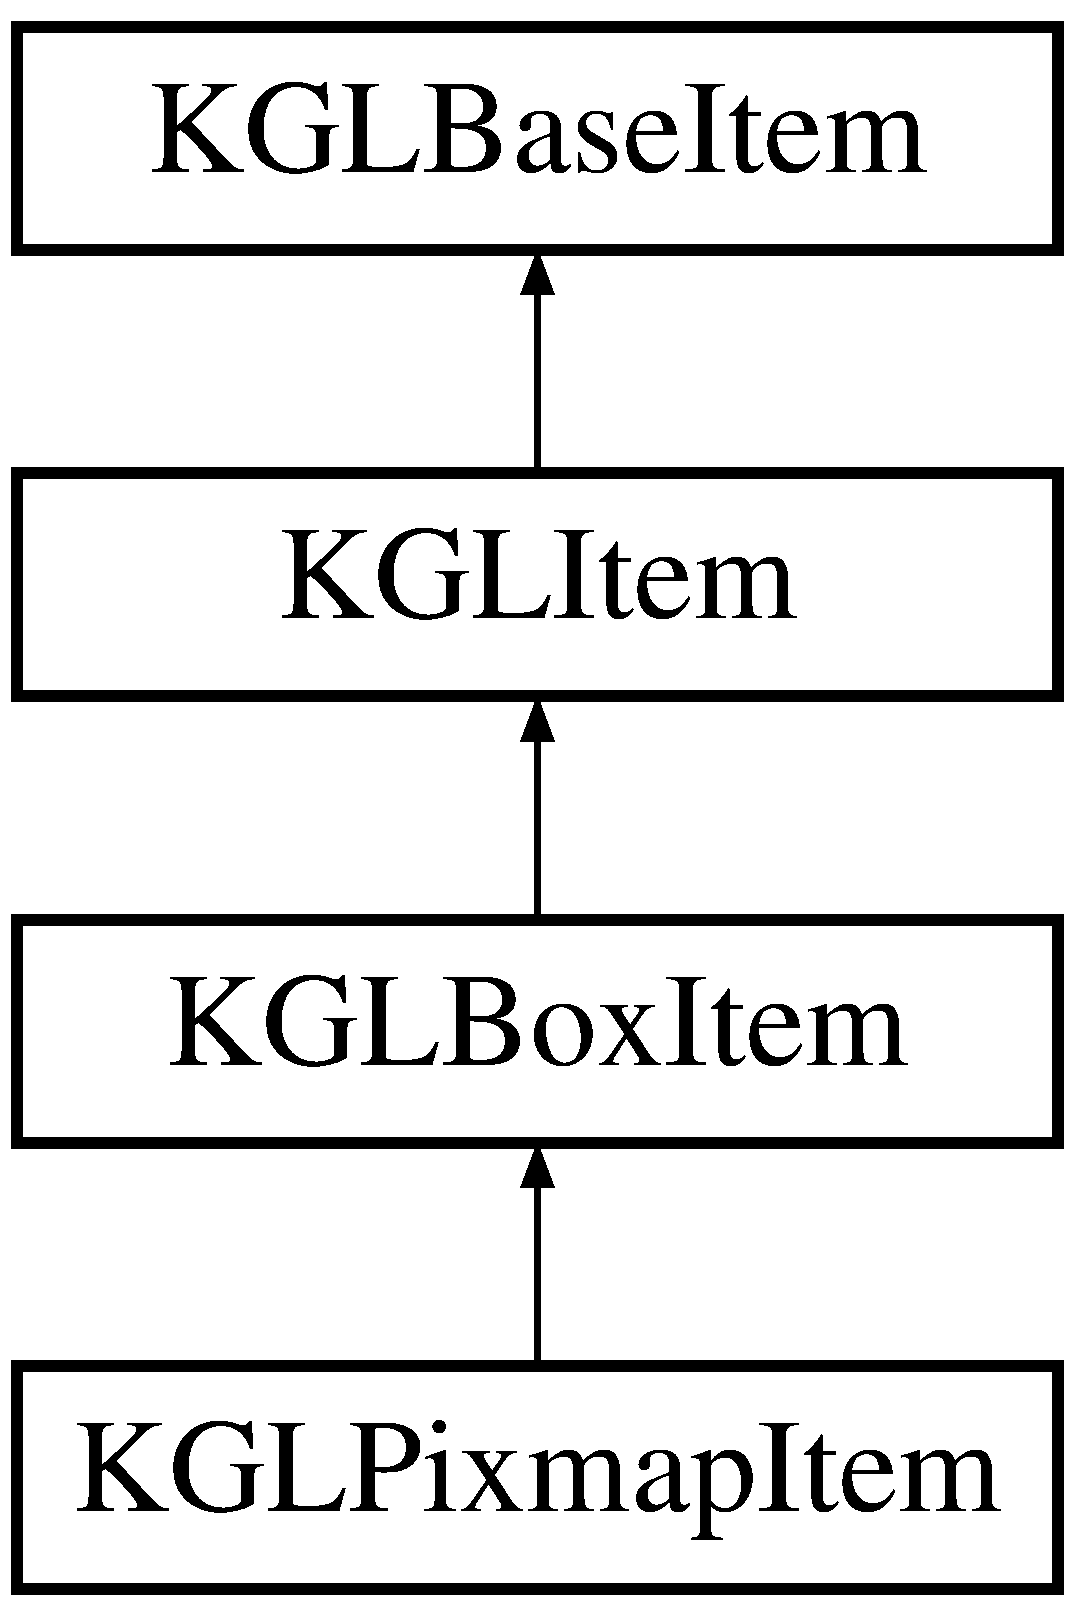
\includegraphics[height=4cm]{class_k_g_l_pixmap_item}
\end{center}
\end{figure}
\subsection*{Public Member Functions}
\begin{CompactItemize}
\item 
\hyperlink{class_k_g_l_pixmap_item_7f12bfbc0c6fe5f89363dae5c800b476}{KGLPixmapItem} (const QString \&fileName, \hyperlink{class_k_g_l_engine}{KGLEngine} $\ast$parent=0)
\item 
\hyperlink{class_k_g_l_pixmap_item_8fe07e2180e081aa135b613388377e70}{KGLPixmapItem} (const QPixmap \&p, \hyperlink{class_k_g_l_engine}{KGLEngine} $\ast$parent=0)
\item 
QPixmap \& \hyperlink{class_k_g_l_pixmap_item_5f5bdbb102070403f1fdbd046b4e0a61}{pixmap} ()
\end{CompactItemize}


\subsection{Constructor \& Destructor Documentation}
\hypertarget{class_k_g_l_pixmap_item_7f12bfbc0c6fe5f89363dae5c800b476}{
\index{KGLPixmapItem@{KGLPixmapItem}!KGLPixmapItem@{KGLPixmapItem}}
\index{KGLPixmapItem@{KGLPixmapItem}!KGLPixmapItem@{KGLPixmapItem}}
\subsubsection[{KGLPixmapItem}]{\setlength{\rightskip}{0pt plus 5cm}KGLPixmapItem::KGLPixmapItem (const QString \& {\em fileName}, \/  {\bf KGLEngine} $\ast$ {\em parent} = {\tt 0})\hspace{0.3cm}{\tt  \mbox{[}explicit\mbox{]}}}}
\label{class_k_g_l_pixmap_item_7f12bfbc0c6fe5f89363dae5c800b476}


\hypertarget{class_k_g_l_pixmap_item_8fe07e2180e081aa135b613388377e70}{
\index{KGLPixmapItem@{KGLPixmapItem}!KGLPixmapItem@{KGLPixmapItem}}
\index{KGLPixmapItem@{KGLPixmapItem}!KGLPixmapItem@{KGLPixmapItem}}
\subsubsection[{KGLPixmapItem}]{\setlength{\rightskip}{0pt plus 5cm}KGLPixmapItem::KGLPixmapItem (const QPixmap \& {\em p}, \/  {\bf KGLEngine} $\ast$ {\em parent} = {\tt 0})\hspace{0.3cm}{\tt  \mbox{[}explicit\mbox{]}}}}
\label{class_k_g_l_pixmap_item_8fe07e2180e081aa135b613388377e70}




\subsection{Member Function Documentation}
\hypertarget{class_k_g_l_pixmap_item_5f5bdbb102070403f1fdbd046b4e0a61}{
\index{KGLPixmapItem@{KGLPixmapItem}!pixmap@{pixmap}}
\index{pixmap@{pixmap}!KGLPixmapItem@{KGLPixmapItem}}
\subsubsection[{pixmap}]{\setlength{\rightskip}{0pt plus 5cm}QPixmap\& KGLPixmapItem::pixmap ()\hspace{0.3cm}{\tt  \mbox{[}inline\mbox{]}}}}
\label{class_k_g_l_pixmap_item_5f5bdbb102070403f1fdbd046b4e0a61}




The documentation for this class was generated from the following files:\begin{CompactItemize}
\item 
/home/sacha/programmation/gluon/kgl/\hyperlink{kglpixmapitem_8h}{kglpixmapitem.h}\item 
/home/sacha/programmation/gluon/kgl/\hyperlink{kglpixmapitem_8cpp}{kglpixmapitem.cpp}\end{CompactItemize}

\hypertarget{class_k_g_l_point}{
\section{KGLPoint Class Reference}
\label{class_k_g_l_point}\index{KGLPoint@{KGLPoint}}
}
{\tt \#include $<$kglpoint.h$>$}

\subsection*{Public Member Functions}
\begin{CompactItemize}
\item 
\hyperlink{class_k_g_l_point_ec90027724e47b130bfa7baa537c3525}{KGLPoint} ()
\item 
\hyperlink{class_k_g_l_point_f07f3a2263c4855e244e07b4008aed3b}{KGLPoint} (const QPointF \&p, const QColor \&c=Qt::white, const QPointF \&t=QPointF())
\item 
\hyperlink{class_k_g_l_point_0c51439bef1f4a13b842fe374d26f67d}{KGLPoint} (float x, float y, const QColor \&c=Qt::white, const QPointF \&t=QPointF())
\item 
QPointF \hyperlink{class_k_g_l_point_75e4837c809e80d80d93df8009a79b39}{tex} ()
\item 
QColor \hyperlink{class_k_g_l_point_12056ee2968beabf1d8cbc1f78fb925d}{color} ()
\item 
void \hyperlink{class_k_g_l_point_2670bdba8e0274cacd1034fa048dbf64}{setTex} (const QPointF \&t)
\item 
void \hyperlink{class_k_g_l_point_b03b0a3565b23a9dc914e877ccde23e9}{setColor} (const QColor \&c)
\item 
void \hyperlink{class_k_g_l_point_8466138efb12c13c8866ea8354f3f839}{setAlpha} (float a)
\item 
QPointF \hyperlink{class_k_g_l_point_91024421e8cca6c1f9752eea9e0f7c91}{toQPointF} ()
\item 
float \hyperlink{class_k_g_l_point_336b4291f8554fdfc29e2c8e37290374}{x} ()
\item 
float \hyperlink{class_k_g_l_point_f13e00b27b57545e193c77f98eed8763}{y} ()
\item 
float \hyperlink{class_k_g_l_point_962653ad291ec2e50e079312963ead48}{red} ()
\item 
float \hyperlink{class_k_g_l_point_5c879ad55c4acfde4a8749391852c7e5}{green} ()
\item 
float \hyperlink{class_k_g_l_point_36413238e5278cf10a8adf0775c646e8}{blue} ()
\item 
float \hyperlink{class_k_g_l_point_638b9d22b3bc3fd7d18d073de199d6f4}{alpha} ()
\item 
float \hyperlink{class_k_g_l_point_997327431417659d02cae5f3c0c91297}{texCoordX} ()
\item 
float \hyperlink{class_k_g_l_point_b9202127decfa0165dc49903a28e6ae9}{texCoordY} ()
\end{CompactItemize}


\subsection{Constructor \& Destructor Documentation}
\hypertarget{class_k_g_l_point_ec90027724e47b130bfa7baa537c3525}{
\index{KGLPoint@{KGLPoint}!KGLPoint@{KGLPoint}}
\index{KGLPoint@{KGLPoint}!KGLPoint@{KGLPoint}}
\subsubsection[{KGLPoint}]{\setlength{\rightskip}{0pt plus 5cm}KGLPoint::KGLPoint ()\hspace{0.3cm}{\tt  \mbox{[}explicit\mbox{]}}}}
\label{class_k_g_l_point_ec90027724e47b130bfa7baa537c3525}


\hypertarget{class_k_g_l_point_f07f3a2263c4855e244e07b4008aed3b}{
\index{KGLPoint@{KGLPoint}!KGLPoint@{KGLPoint}}
\index{KGLPoint@{KGLPoint}!KGLPoint@{KGLPoint}}
\subsubsection[{KGLPoint}]{\setlength{\rightskip}{0pt plus 5cm}KGLPoint::KGLPoint (const QPointF \& {\em p}, \/  const QColor \& {\em c} = {\tt Qt::white}, \/  const QPointF \& {\em t} = {\tt QPointF()})\hspace{0.3cm}{\tt  \mbox{[}explicit\mbox{]}}}}
\label{class_k_g_l_point_f07f3a2263c4855e244e07b4008aed3b}


\hypertarget{class_k_g_l_point_0c51439bef1f4a13b842fe374d26f67d}{
\index{KGLPoint@{KGLPoint}!KGLPoint@{KGLPoint}}
\index{KGLPoint@{KGLPoint}!KGLPoint@{KGLPoint}}
\subsubsection[{KGLPoint}]{\setlength{\rightskip}{0pt plus 5cm}KGLPoint::KGLPoint (float {\em x}, \/  float {\em y}, \/  const QColor \& {\em c} = {\tt Qt::white}, \/  const QPointF \& {\em t} = {\tt QPointF()})\hspace{0.3cm}{\tt  \mbox{[}explicit\mbox{]}}}}
\label{class_k_g_l_point_0c51439bef1f4a13b842fe374d26f67d}




\subsection{Member Function Documentation}
\hypertarget{class_k_g_l_point_638b9d22b3bc3fd7d18d073de199d6f4}{
\index{KGLPoint@{KGLPoint}!alpha@{alpha}}
\index{alpha@{alpha}!KGLPoint@{KGLPoint}}
\subsubsection[{alpha}]{\setlength{\rightskip}{0pt plus 5cm}float KGLPoint::alpha ()\hspace{0.3cm}{\tt  \mbox{[}inline\mbox{]}}}}
\label{class_k_g_l_point_638b9d22b3bc3fd7d18d073de199d6f4}


\hypertarget{class_k_g_l_point_36413238e5278cf10a8adf0775c646e8}{
\index{KGLPoint@{KGLPoint}!blue@{blue}}
\index{blue@{blue}!KGLPoint@{KGLPoint}}
\subsubsection[{blue}]{\setlength{\rightskip}{0pt plus 5cm}float KGLPoint::blue ()\hspace{0.3cm}{\tt  \mbox{[}inline\mbox{]}}}}
\label{class_k_g_l_point_36413238e5278cf10a8adf0775c646e8}


\hypertarget{class_k_g_l_point_12056ee2968beabf1d8cbc1f78fb925d}{
\index{KGLPoint@{KGLPoint}!color@{color}}
\index{color@{color}!KGLPoint@{KGLPoint}}
\subsubsection[{color}]{\setlength{\rightskip}{0pt plus 5cm}QColor KGLPoint::color ()\hspace{0.3cm}{\tt  \mbox{[}inline\mbox{]}}}}
\label{class_k_g_l_point_12056ee2968beabf1d8cbc1f78fb925d}


\hypertarget{class_k_g_l_point_5c879ad55c4acfde4a8749391852c7e5}{
\index{KGLPoint@{KGLPoint}!green@{green}}
\index{green@{green}!KGLPoint@{KGLPoint}}
\subsubsection[{green}]{\setlength{\rightskip}{0pt plus 5cm}float KGLPoint::green ()\hspace{0.3cm}{\tt  \mbox{[}inline\mbox{]}}}}
\label{class_k_g_l_point_5c879ad55c4acfde4a8749391852c7e5}


\hypertarget{class_k_g_l_point_962653ad291ec2e50e079312963ead48}{
\index{KGLPoint@{KGLPoint}!red@{red}}
\index{red@{red}!KGLPoint@{KGLPoint}}
\subsubsection[{red}]{\setlength{\rightskip}{0pt plus 5cm}float KGLPoint::red ()\hspace{0.3cm}{\tt  \mbox{[}inline\mbox{]}}}}
\label{class_k_g_l_point_962653ad291ec2e50e079312963ead48}


\hypertarget{class_k_g_l_point_8466138efb12c13c8866ea8354f3f839}{
\index{KGLPoint@{KGLPoint}!setAlpha@{setAlpha}}
\index{setAlpha@{setAlpha}!KGLPoint@{KGLPoint}}
\subsubsection[{setAlpha}]{\setlength{\rightskip}{0pt plus 5cm}void KGLPoint::setAlpha (float {\em a})\hspace{0.3cm}{\tt  \mbox{[}inline\mbox{]}}}}
\label{class_k_g_l_point_8466138efb12c13c8866ea8354f3f839}


\hypertarget{class_k_g_l_point_b03b0a3565b23a9dc914e877ccde23e9}{
\index{KGLPoint@{KGLPoint}!setColor@{setColor}}
\index{setColor@{setColor}!KGLPoint@{KGLPoint}}
\subsubsection[{setColor}]{\setlength{\rightskip}{0pt plus 5cm}void KGLPoint::setColor (const QColor \& {\em c})\hspace{0.3cm}{\tt  \mbox{[}inline\mbox{]}}}}
\label{class_k_g_l_point_b03b0a3565b23a9dc914e877ccde23e9}


\hypertarget{class_k_g_l_point_2670bdba8e0274cacd1034fa048dbf64}{
\index{KGLPoint@{KGLPoint}!setTex@{setTex}}
\index{setTex@{setTex}!KGLPoint@{KGLPoint}}
\subsubsection[{setTex}]{\setlength{\rightskip}{0pt plus 5cm}void KGLPoint::setTex (const QPointF \& {\em t})\hspace{0.3cm}{\tt  \mbox{[}inline\mbox{]}}}}
\label{class_k_g_l_point_2670bdba8e0274cacd1034fa048dbf64}


\hypertarget{class_k_g_l_point_75e4837c809e80d80d93df8009a79b39}{
\index{KGLPoint@{KGLPoint}!tex@{tex}}
\index{tex@{tex}!KGLPoint@{KGLPoint}}
\subsubsection[{tex}]{\setlength{\rightskip}{0pt plus 5cm}QPointF KGLPoint::tex ()\hspace{0.3cm}{\tt  \mbox{[}inline\mbox{]}}}}
\label{class_k_g_l_point_75e4837c809e80d80d93df8009a79b39}


\hypertarget{class_k_g_l_point_997327431417659d02cae5f3c0c91297}{
\index{KGLPoint@{KGLPoint}!texCoordX@{texCoordX}}
\index{texCoordX@{texCoordX}!KGLPoint@{KGLPoint}}
\subsubsection[{texCoordX}]{\setlength{\rightskip}{0pt plus 5cm}float KGLPoint::texCoordX ()\hspace{0.3cm}{\tt  \mbox{[}inline\mbox{]}}}}
\label{class_k_g_l_point_997327431417659d02cae5f3c0c91297}


\hypertarget{class_k_g_l_point_b9202127decfa0165dc49903a28e6ae9}{
\index{KGLPoint@{KGLPoint}!texCoordY@{texCoordY}}
\index{texCoordY@{texCoordY}!KGLPoint@{KGLPoint}}
\subsubsection[{texCoordY}]{\setlength{\rightskip}{0pt plus 5cm}float KGLPoint::texCoordY ()\hspace{0.3cm}{\tt  \mbox{[}inline\mbox{]}}}}
\label{class_k_g_l_point_b9202127decfa0165dc49903a28e6ae9}


\hypertarget{class_k_g_l_point_91024421e8cca6c1f9752eea9e0f7c91}{
\index{KGLPoint@{KGLPoint}!toQPointF@{toQPointF}}
\index{toQPointF@{toQPointF}!KGLPoint@{KGLPoint}}
\subsubsection[{toQPointF}]{\setlength{\rightskip}{0pt plus 5cm}QPointF KGLPoint::toQPointF ()\hspace{0.3cm}{\tt  \mbox{[}inline\mbox{]}}}}
\label{class_k_g_l_point_91024421e8cca6c1f9752eea9e0f7c91}


\hypertarget{class_k_g_l_point_336b4291f8554fdfc29e2c8e37290374}{
\index{KGLPoint@{KGLPoint}!x@{x}}
\index{x@{x}!KGLPoint@{KGLPoint}}
\subsubsection[{x}]{\setlength{\rightskip}{0pt plus 5cm}float KGLPoint::x ()\hspace{0.3cm}{\tt  \mbox{[}inline\mbox{]}}}}
\label{class_k_g_l_point_336b4291f8554fdfc29e2c8e37290374}


\hypertarget{class_k_g_l_point_f13e00b27b57545e193c77f98eed8763}{
\index{KGLPoint@{KGLPoint}!y@{y}}
\index{y@{y}!KGLPoint@{KGLPoint}}
\subsubsection[{y}]{\setlength{\rightskip}{0pt plus 5cm}float KGLPoint::y ()\hspace{0.3cm}{\tt  \mbox{[}inline\mbox{]}}}}
\label{class_k_g_l_point_f13e00b27b57545e193c77f98eed8763}




The documentation for this class was generated from the following files:\begin{CompactItemize}
\item 
/home/sacha/programmation/gluon/kgl/\hyperlink{kglpoint_8h}{kglpoint.h}\item 
/home/sacha/programmation/gluon/kgl/\hyperlink{kglpoint_8cpp}{kglpoint.cpp}\end{CompactItemize}

\hypertarget{class_k_g_l_point_list}{
\section{KGLPointList Class Reference}
\label{class_k_g_l_point_list}\index{KGLPointList@{KGLPointList}}
}
{\tt \#include $<$kglpoint.h$>$}

\subsection*{Public Member Functions}
\begin{CompactItemize}
\item 
\hyperlink{class_k_g_l_point_list_c714e47e8f2b86382ecc248b2d7b94b2}{KGLPointList} ()
\item 
float $\ast$ \hyperlink{class_k_g_l_point_list_3ad82d96624e2dc59dbb3d8688d50209}{array} ()
\item 
float $\ast$ \hyperlink{class_k_g_l_point_list_66f55a46c09cc9062c5a62279a936a09}{vertexStart} ()
\item 
float $\ast$ \hyperlink{class_k_g_l_point_list_68ee14e7429f2390b8dd7dbb3492dec3}{colorStart} ()
\item 
float $\ast$ \hyperlink{class_k_g_l_point_list_173fb946e98e011a010eecaf8fb10dbf}{texCoordStart} ()
\end{CompactItemize}


\subsection{Constructor \& Destructor Documentation}
\hypertarget{class_k_g_l_point_list_c714e47e8f2b86382ecc248b2d7b94b2}{
\index{KGLPointList@{KGLPointList}!KGLPointList@{KGLPointList}}
\index{KGLPointList@{KGLPointList}!KGLPointList@{KGLPointList}}
\subsubsection[{KGLPointList}]{\setlength{\rightskip}{0pt plus 5cm}KGLPointList::KGLPointList ()}}
\label{class_k_g_l_point_list_c714e47e8f2b86382ecc248b2d7b94b2}




\subsection{Member Function Documentation}
\hypertarget{class_k_g_l_point_list_3ad82d96624e2dc59dbb3d8688d50209}{
\index{KGLPointList@{KGLPointList}!array@{array}}
\index{array@{array}!KGLPointList@{KGLPointList}}
\subsubsection[{array}]{\setlength{\rightskip}{0pt plus 5cm}float$\ast$ KGLPointList::array ()\hspace{0.3cm}{\tt  \mbox{[}inline\mbox{]}}}}
\label{class_k_g_l_point_list_3ad82d96624e2dc59dbb3d8688d50209}


\hypertarget{class_k_g_l_point_list_68ee14e7429f2390b8dd7dbb3492dec3}{
\index{KGLPointList@{KGLPointList}!colorStart@{colorStart}}
\index{colorStart@{colorStart}!KGLPointList@{KGLPointList}}
\subsubsection[{colorStart}]{\setlength{\rightskip}{0pt plus 5cm}float$\ast$ KGLPointList::colorStart ()\hspace{0.3cm}{\tt  \mbox{[}inline\mbox{]}}}}
\label{class_k_g_l_point_list_68ee14e7429f2390b8dd7dbb3492dec3}


\hypertarget{class_k_g_l_point_list_173fb946e98e011a010eecaf8fb10dbf}{
\index{KGLPointList@{KGLPointList}!texCoordStart@{texCoordStart}}
\index{texCoordStart@{texCoordStart}!KGLPointList@{KGLPointList}}
\subsubsection[{texCoordStart}]{\setlength{\rightskip}{0pt plus 5cm}float$\ast$ KGLPointList::texCoordStart ()\hspace{0.3cm}{\tt  \mbox{[}inline\mbox{]}}}}
\label{class_k_g_l_point_list_173fb946e98e011a010eecaf8fb10dbf}


\hypertarget{class_k_g_l_point_list_66f55a46c09cc9062c5a62279a936a09}{
\index{KGLPointList@{KGLPointList}!vertexStart@{vertexStart}}
\index{vertexStart@{vertexStart}!KGLPointList@{KGLPointList}}
\subsubsection[{vertexStart}]{\setlength{\rightskip}{0pt plus 5cm}float$\ast$ KGLPointList::vertexStart ()\hspace{0.3cm}{\tt  \mbox{[}inline\mbox{]}}}}
\label{class_k_g_l_point_list_66f55a46c09cc9062c5a62279a936a09}




The documentation for this class was generated from the following files:\begin{CompactItemize}
\item 
/home/sacha/programmation/gluon/kgl/\hyperlink{kglpoint_8h}{kglpoint.h}\item 
/home/sacha/programmation/gluon/kgl/\hyperlink{kglpoint_8cpp}{kglpoint.cpp}\end{CompactItemize}

\hypertarget{class_k_g_l_polygon_item}{
\section{KGLPolygonItem Class Reference}
\label{class_k_g_l_polygon_item}\index{KGLPolygonItem@{KGLPolygonItem}}
}
{\tt \#include $<$KGLPolygonItem$>$}

Inheritance diagram for KGLPolygonItem::\begin{figure}[H]
\begin{center}
\leavevmode
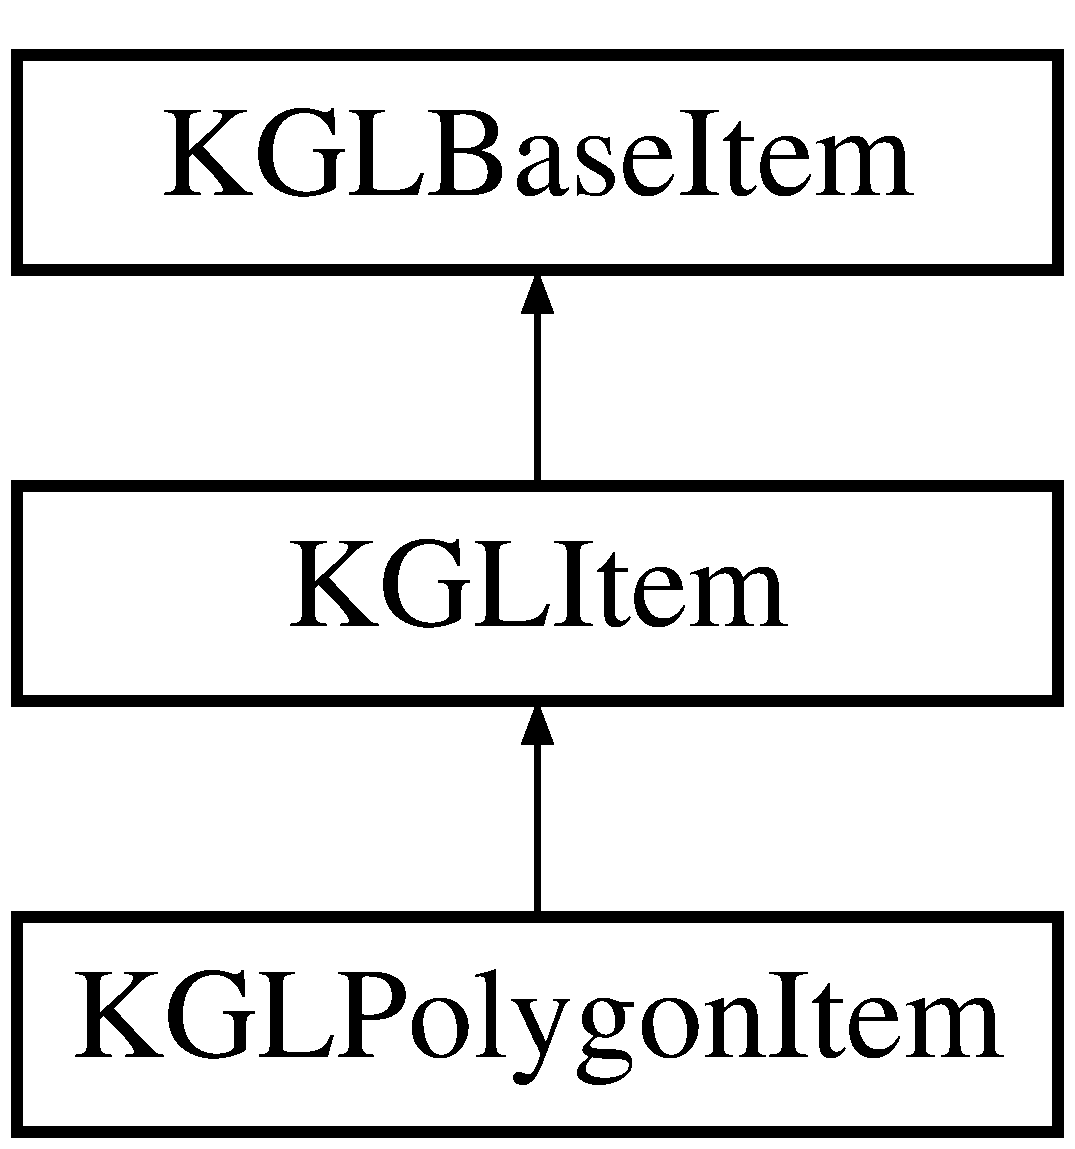
\includegraphics[height=3cm]{class_k_g_l_polygon_item}
\end{center}
\end{figure}
\subsection*{Public Member Functions}
\begin{CompactItemize}
\item 
\hyperlink{class_k_g_l_polygon_item_5623294ed1300654c22c960384c39e62}{KGLPolygonItem} (const QPolygonF \&polygon, \hyperlink{class_k_g_l_engine}{KGLEngine} $\ast$parent=0)
\end{CompactItemize}


\subsection{Detailed Description}
This is a \hyperlink{class_k_g_l_item}{KGLItem} subclass that represents a polygon, and which can be initialized with a QPolygonF. 

\subsection{Constructor \& Destructor Documentation}
\hypertarget{class_k_g_l_polygon_item_5623294ed1300654c22c960384c39e62}{
\index{KGLPolygonItem@{KGLPolygonItem}!KGLPolygonItem@{KGLPolygonItem}}
\index{KGLPolygonItem@{KGLPolygonItem}!KGLPolygonItem@{KGLPolygonItem}}
\subsubsection[{KGLPolygonItem}]{\setlength{\rightskip}{0pt plus 5cm}KGLPolygonItem::KGLPolygonItem (const QPolygonF \& {\em polygon}, \/  {\bf KGLEngine} $\ast$ {\em parent} = {\tt 0})}}
\label{class_k_g_l_polygon_item_5623294ed1300654c22c960384c39e62}




The documentation for this class was generated from the following files:\begin{CompactItemize}
\item 
/home/sacha/programmation/gluon/kgl/\hyperlink{kglpolygonitem_8h}{kglpolygonitem.h}\item 
/home/sacha/programmation/gluon/kgl/\hyperlink{kglpolygonitem_8cpp}{kglpolygonitem.cpp}\end{CompactItemize}

\hypertarget{class_k_g_l_program}{
\section{KGLProgram Class Reference}
\label{class_k_g_l_program}\index{KGLProgram@{KGLProgram}}
}
Program class.  


{\tt \#include $<$kglprogram.h$>$}

\subsection*{Public Member Functions}
\begin{CompactItemize}
\item 
\hyperlink{class_k_g_l_program_e252511a4efad9a198d44a0a69b0f43b}{KGLProgram} ()
\item 
\hyperlink{class_k_g_l_program_a72b7b0ac0efba795712e2e72e067127}{KGLProgram} (const QList$<$ \hyperlink{class_k_g_l_shader}{KGLShader} $\ast$ $>$ \&shaders)
\item 
\hyperlink{class_k_g_l_program_ed56f8e432d8e523deab848515b04bea}{KGLProgram} (const QString \&vertexshaderfile, const QString \&fragmentshaderfile)
\item 
virtual \hyperlink{class_k_g_l_program_2c90a7ed95bc53b2766e556c1ca996cb}{$\sim$KGLProgram} ()
\item 
void \hyperlink{class_k_g_l_program_cb58b41949d3a88b66557f43196dcaba}{addShader} (\hyperlink{class_k_g_l_shader}{KGLShader} $\ast$shader)
\item 
void \hyperlink{class_k_g_l_program_465ecaf07d2116b74bf892d40c7dc17a}{addShaders} (const QList$<$ \hyperlink{class_k_g_l_shader}{KGLShader} $\ast$ $>$ \&shaders)
\item 
virtual bool \hyperlink{class_k_g_l_program_906166edf1fc7332a5ff8d6c1c18469c}{link} ()
\item 
bool \hyperlink{class_k_g_l_program_5c1aeee12f117bcdb9617ef27c223918}{isValid} () const 
\item 
char $\ast$ \hyperlink{class_k_g_l_program_731506a0e8462aa48f576ab4c1d28fc9}{linkLog} () const 
\item 
virtual void \hyperlink{class_k_g_l_program_48756f0c04a768d2fef06d7ac3d29207}{bind} () const 
\item 
virtual void \hyperlink{class_k_g_l_program_a52890b41224848903a772049f374dc3}{unbind} () const 
\item 
int \hyperlink{class_k_g_l_program_51a6b83fc54f4364ae013068823a981d}{uniformLocation} (const QString \&name)
\item 
int \hyperlink{class_k_g_l_program_9e38df2dc72639004319fef0c169e3c9}{uniformLocation} (const char $\ast$name)
\item 
int \hyperlink{class_k_g_l_program_16d1cc930ef9585ec503fe935c4b6a9f}{attributeLocation} (const QString \&name)
\item 
int \hyperlink{class_k_g_l_program_237f2223b1ba1c80e90543d0523739c4}{attributeLocation} (const char $\ast$name)
\item 
void \hyperlink{class_k_g_l_program_949c83395eed27219fd984fe33ac9ecf}{invalidateLocations} ()
\item 
bool \hyperlink{class_k_g_l_program_6704e664e129126050b6f5609da1ee61}{setUniform} (const char $\ast$name, float value)
\item 
bool \hyperlink{class_k_g_l_program_a3213a9de09529704183cb61bec910d4}{setUniform} (const char $\ast$name, Eigen::Vector2f value)
\item 
bool \hyperlink{class_k_g_l_program_e971d4c55c57ae853f4d1c8cdd8a22b9}{setUniform} (const char $\ast$name, Eigen::Vector3f value)
\item 
bool \hyperlink{class_k_g_l_program_b5a31ac9ea1f50767144233afaa0a9e3}{setUniform} (const char $\ast$name, Eigen::Vector4f value)
\item 
bool \hyperlink{class_k_g_l_program_4d943d685f583e9a446d44689b6e7b0c}{setUniform} (const char $\ast$name, int value)
\item 
GLuint \hyperlink{class_k_g_l_program_7a9b4ef4da3e149386a50c8d4241b6c6}{glId} () const 
\end{CompactItemize}
\subsection*{Protected Member Functions}
\begin{CompactItemize}
\item 
void \hyperlink{class_k_g_l_program_5c8081f85275e023d6bf034d54bd1721}{init} ()
\end{CompactItemize}
\subsection*{Protected Attributes}
\begin{CompactItemize}
\item 
GLuint \hyperlink{class_k_g_l_program_1200bdd28e580ca66b818dbefee24f22}{mGLId}
\item 
bool \hyperlink{class_k_g_l_program_f228db2a0bcddd2366e1353b25a193dc}{mValid}
\item 
char $\ast$ \hyperlink{class_k_g_l_program_af8102a5a3f4c7bb21f3f0c56c6806a4}{mLinkLog}
\item 
QHash$<$ QString, int $>$ $\ast$ \hyperlink{class_k_g_l_program_b6b870ec76b667369f457cc980e9016c}{mUniformLocations}
\item 
QHash$<$ QString, int $>$ $\ast$ \hyperlink{class_k_g_l_program_7ebfd6e8476719c40d24108a043d7bd1}{mAttributeLocations}
\end{CompactItemize}


\subsection{Detailed Description}
Program class. 

Program is a GPU-executed program that is ready to be used for manipulating geometry and colors. Program can encapsulate vertex and fragment shaders or just one of them. If only either vertex or fragment shader is used, then traditional fixed-function pipeline is used for the other stage.\hypertarget{class_k_g_l_program_creating}{}\subsection{Creating Program objects}\label{class_k_g_l_program_creating}
The easiest way to create usable Program object is to pass filenames of the vertex- and fragment shader to the Program constructor. This automatically creates temporary Shader objects and then combines them into a Program: 

\begin{Code}\begin{verbatim} Program* prog = new Program("myshader.vert", "myshader.frag");
 if (!prog->isValid()) {
     // Error: program failed to load
 }
\end{verbatim}
\end{Code}



It is also possible to add more than one fragment or vertex shader (e.g. you can have some common functions in one shader and the main() function in other) or specify only vertex or only fragment shader. In this case you will have to first create the Shader objects yourself and then add them to a program: 

\begin{Code}\begin{verbatim} // Create Shader objects
 VertexShader vertexShader("myshader.vert");
 FragmentShader fragmentShader("myshader.frag");
 // common.frag could contain common functions shared by different shaders
 FragmentShader commonShader("common.frag");
 // Make sure all shaders were successfully loaded
 if (!vertexShader.isValid() || !fragmentShader.isValid() || !commonShader.isValid()) {
     // handle the error here
     return;
 }

 // Create Program object
 Program* prog = new Program();
 // Add shader objects to program
 prog->addShader(&vertexShader);
 prog->addShader(&fragmentShader);
 prog->addShader(&commonShader);
 // Finally link them together
 prog->link();
 // And make sure everything succeeded
 if (!prog->isValid()) {
     // handle the error
 }
\end{verbatim}
\end{Code}

\hypertarget{class_k_g_l_program_binding}{}\subsection{Binding}\label{class_k_g_l_program_binding}
To use the program, you need to first \hyperlink{class_k_g_l_program_48756f0c04a768d2fef06d7ac3d29207}{bind()} it, then render your geometry and finally \hyperlink{class_k_g_l_program_a52890b41224848903a772049f374dc3}{unbind()} it. Note that it's more convenient to use the Mesh class which takes care of the binding and unbinding automatically. 

\begin{Code}\begin{verbatim} prog->bind();
 // Everything rendered now will use the bound program
 renderObjects();
 // Finally unbind the program
 prog->unbind();
\end{verbatim}
\end{Code}

\hypertarget{class_k_g_l_program_uniforms}{}\subsection{Uniform variables}\label{class_k_g_l_program_uniforms}
For communication between GPU Program and your main application, uniform variables can be used. They can be written from your main program and read in shader code. Note that modifying values of uniform variables may be expensive, thus you should do it only when really necessary. 

\begin{Code}\begin{verbatim} // The program has to be bound before setUniform() can be used
 prog->bind();
 // Set variable "objectScale" to 2.0f
 prog->setUniform("objectScale", 2.0f);
 // Unbind the program
 prog->unbind();
\end{verbatim}
\end{Code}



The corresponding section in the shader code would look like this: 

\begin{Code}\begin{verbatim} uniform float objectScale;
 // objectScale can now be used as any other variable
\end{verbatim}
\end{Code}



\begin{Desc}
\item[See also:]Shader, Mesh \end{Desc}


\subsection{Constructor \& Destructor Documentation}
\hypertarget{class_k_g_l_program_e252511a4efad9a198d44a0a69b0f43b}{
\index{KGLProgram@{KGLProgram}!KGLProgram@{KGLProgram}}
\index{KGLProgram@{KGLProgram}!KGLProgram@{KGLProgram}}
\subsubsection[{KGLProgram}]{\setlength{\rightskip}{0pt plus 5cm}KGLProgram::KGLProgram ()}}
\label{class_k_g_l_program_e252511a4efad9a198d44a0a69b0f43b}


Creates empty Program. You will need to add some shaders and link the program before you can use it. \hypertarget{class_k_g_l_program_a72b7b0ac0efba795712e2e72e067127}{
\index{KGLProgram@{KGLProgram}!KGLProgram@{KGLProgram}}
\index{KGLProgram@{KGLProgram}!KGLProgram@{KGLProgram}}
\subsubsection[{KGLProgram}]{\setlength{\rightskip}{0pt plus 5cm}KGLProgram::KGLProgram (const QList$<$ {\bf KGLShader} $\ast$ $>$ \& {\em shaders})}}
\label{class_k_g_l_program_a72b7b0ac0efba795712e2e72e067127}


Creates Program, adds given list of shaders and links the program. If linking succeeded, the program is ready to be used. \hypertarget{class_k_g_l_program_ed56f8e432d8e523deab848515b04bea}{
\index{KGLProgram@{KGLProgram}!KGLProgram@{KGLProgram}}
\index{KGLProgram@{KGLProgram}!KGLProgram@{KGLProgram}}
\subsubsection[{KGLProgram}]{\setlength{\rightskip}{0pt plus 5cm}KGLProgram::KGLProgram (const QString \& {\em vertexshaderfile}, \/  const QString \& {\em fragmentshaderfile})}}
\label{class_k_g_l_program_ed56f8e432d8e523deab848515b04bea}


Loads vertex and fragment shaders from given files, adds them and links the program. If everything succeeded, then the program is ready to be used. \hypertarget{class_k_g_l_program_2c90a7ed95bc53b2766e556c1ca996cb}{
\index{KGLProgram@{KGLProgram}!$\sim$KGLProgram@{$\sim$KGLProgram}}
\index{$\sim$KGLProgram@{$\sim$KGLProgram}!KGLProgram@{KGLProgram}}
\subsubsection[{$\sim$KGLProgram}]{\setlength{\rightskip}{0pt plus 5cm}KGLProgram::$\sim$KGLProgram ()\hspace{0.3cm}{\tt  \mbox{[}virtual\mbox{]}}}}
\label{class_k_g_l_program_2c90a7ed95bc53b2766e556c1ca996cb}


Deletes this library and frees all resources. 

\subsection{Member Function Documentation}
\hypertarget{class_k_g_l_program_cb58b41949d3a88b66557f43196dcaba}{
\index{KGLProgram@{KGLProgram}!addShader@{addShader}}
\index{addShader@{addShader}!KGLProgram@{KGLProgram}}
\subsubsection[{addShader}]{\setlength{\rightskip}{0pt plus 5cm}void KGLProgram::addShader ({\bf KGLShader} $\ast$ {\em shader})}}
\label{class_k_g_l_program_cb58b41949d3a88b66557f43196dcaba}


Adds given shader to this library. \hypertarget{class_k_g_l_program_465ecaf07d2116b74bf892d40c7dc17a}{
\index{KGLProgram@{KGLProgram}!addShaders@{addShaders}}
\index{addShaders@{addShaders}!KGLProgram@{KGLProgram}}
\subsubsection[{addShaders}]{\setlength{\rightskip}{0pt plus 5cm}void KGLProgram::addShaders (const QList$<$ {\bf KGLShader} $\ast$ $>$ \& {\em shaders})}}
\label{class_k_g_l_program_465ecaf07d2116b74bf892d40c7dc17a}


Adds all shaders in the given list to this library. \hypertarget{class_k_g_l_program_237f2223b1ba1c80e90543d0523739c4}{
\index{KGLProgram@{KGLProgram}!attributeLocation@{attributeLocation}}
\index{attributeLocation@{attributeLocation}!KGLProgram@{KGLProgram}}
\subsubsection[{attributeLocation}]{\setlength{\rightskip}{0pt plus 5cm}int KGLProgram::attributeLocation (const char $\ast$ {\em name})}}
\label{class_k_g_l_program_237f2223b1ba1c80e90543d0523739c4}


\hypertarget{class_k_g_l_program_16d1cc930ef9585ec503fe935c4b6a9f}{
\index{KGLProgram@{KGLProgram}!attributeLocation@{attributeLocation}}
\index{attributeLocation@{attributeLocation}!KGLProgram@{KGLProgram}}
\subsubsection[{attributeLocation}]{\setlength{\rightskip}{0pt plus 5cm}int KGLProgram::attributeLocation (const QString \& {\em name})}}
\label{class_k_g_l_program_16d1cc930ef9585ec503fe935c4b6a9f}


\hypertarget{class_k_g_l_program_48756f0c04a768d2fef06d7ac3d29207}{
\index{KGLProgram@{KGLProgram}!bind@{bind}}
\index{bind@{bind}!KGLProgram@{KGLProgram}}
\subsubsection[{bind}]{\setlength{\rightskip}{0pt plus 5cm}void KGLProgram::bind () const\hspace{0.3cm}{\tt  \mbox{[}virtual\mbox{]}}}}
\label{class_k_g_l_program_48756f0c04a768d2fef06d7ac3d29207}


Binds the program so that it will be used for anything that is rendered after the \hyperlink{class_k_g_l_program_48756f0c04a768d2fef06d7ac3d29207}{bind()} call.

\begin{Desc}
\item[See also:]\hyperlink{class_k_g_l_program_a52890b41224848903a772049f374dc3}{unbind()} \end{Desc}
\hypertarget{class_k_g_l_program_7a9b4ef4da3e149386a50c8d4241b6c6}{
\index{KGLProgram@{KGLProgram}!glId@{glId}}
\index{glId@{glId}!KGLProgram@{KGLProgram}}
\subsubsection[{glId}]{\setlength{\rightskip}{0pt plus 5cm}GLuint KGLProgram::glId () const\hspace{0.3cm}{\tt  \mbox{[}inline\mbox{]}}}}
\label{class_k_g_l_program_7a9b4ef4da3e149386a50c8d4241b6c6}


\begin{Desc}
\item[Returns:]OpenGL id (aka handle) of this library. \end{Desc}
\hypertarget{class_k_g_l_program_5c8081f85275e023d6bf034d54bd1721}{
\index{KGLProgram@{KGLProgram}!init@{init}}
\index{init@{init}!KGLProgram@{KGLProgram}}
\subsubsection[{init}]{\setlength{\rightskip}{0pt plus 5cm}void KGLProgram::init ()\hspace{0.3cm}{\tt  \mbox{[}protected\mbox{]}}}}
\label{class_k_g_l_program_5c8081f85275e023d6bf034d54bd1721}


\hypertarget{class_k_g_l_program_949c83395eed27219fd984fe33ac9ecf}{
\index{KGLProgram@{KGLProgram}!invalidateLocations@{invalidateLocations}}
\index{invalidateLocations@{invalidateLocations}!KGLProgram@{KGLProgram}}
\subsubsection[{invalidateLocations}]{\setlength{\rightskip}{0pt plus 5cm}void KGLProgram::invalidateLocations ()}}
\label{class_k_g_l_program_949c83395eed27219fd984fe33ac9ecf}


\hypertarget{class_k_g_l_program_5c1aeee12f117bcdb9617ef27c223918}{
\index{KGLProgram@{KGLProgram}!isValid@{isValid}}
\index{isValid@{isValid}!KGLProgram@{KGLProgram}}
\subsubsection[{isValid}]{\setlength{\rightskip}{0pt plus 5cm}bool KGLProgram::isValid () const\hspace{0.3cm}{\tt  \mbox{[}inline\mbox{]}}}}
\label{class_k_g_l_program_5c1aeee12f117bcdb9617ef27c223918}


Returns true if this library can be used for rendering, false otherwise.

Invalid programs can be result of syntax errors in the shader code. Program which hasn't been linked yet is also invalid.

\begin{Desc}
\item[See also:]\hyperlink{class_k_g_l_program_906166edf1fc7332a5ff8d6c1c18469c}{link()}, \hyperlink{class_k_g_l_program_731506a0e8462aa48f576ab4c1d28fc9}{linkLog()} \end{Desc}
\hypertarget{class_k_g_l_program_906166edf1fc7332a5ff8d6c1c18469c}{
\index{KGLProgram@{KGLProgram}!link@{link}}
\index{link@{link}!KGLProgram@{KGLProgram}}
\subsubsection[{link}]{\setlength{\rightskip}{0pt plus 5cm}bool KGLProgram::link ()\hspace{0.3cm}{\tt  \mbox{[}virtual\mbox{]}}}}
\label{class_k_g_l_program_906166edf1fc7332a5ff8d6c1c18469c}


Tries to link the shader. If it succeeds, then the program is ready to be used. If there are errors, they should be visible in the \hyperlink{class_k_g_l_program_731506a0e8462aa48f576ab4c1d28fc9}{linkLog}. \begin{Desc}
\item[Returns:]whether linking succeeded. \end{Desc}
\hypertarget{class_k_g_l_program_731506a0e8462aa48f576ab4c1d28fc9}{
\index{KGLProgram@{KGLProgram}!linkLog@{linkLog}}
\index{linkLog@{linkLog}!KGLProgram@{KGLProgram}}
\subsubsection[{linkLog}]{\setlength{\rightskip}{0pt plus 5cm}char$\ast$ KGLProgram::linkLog () const\hspace{0.3cm}{\tt  \mbox{[}inline\mbox{]}}}}
\label{class_k_g_l_program_731506a0e8462aa48f576ab4c1d28fc9}


\begin{Desc}
\item[Returns:]Link log of the program or null if there was none or the program hasn't been linked yet. Note that Program keeps ownership of the returned string, so you mustn't delete it. TODO: maybe return QString? \end{Desc}
\hypertarget{class_k_g_l_program_4d943d685f583e9a446d44689b6e7b0c}{
\index{KGLProgram@{KGLProgram}!setUniform@{setUniform}}
\index{setUniform@{setUniform}!KGLProgram@{KGLProgram}}
\subsubsection[{setUniform}]{\setlength{\rightskip}{0pt plus 5cm}bool KGLProgram::setUniform (const char $\ast$ {\em name}, \/  int {\em value})}}
\label{class_k_g_l_program_4d943d685f583e9a446d44689b6e7b0c}


This is an overloaded member function, provided for convenience. It differs from the above function only in what argument(s) it accepts. \hypertarget{class_k_g_l_program_b5a31ac9ea1f50767144233afaa0a9e3}{
\index{KGLProgram@{KGLProgram}!setUniform@{setUniform}}
\index{setUniform@{setUniform}!KGLProgram@{KGLProgram}}
\subsubsection[{setUniform}]{\setlength{\rightskip}{0pt plus 5cm}bool KGLProgram::setUniform (const char $\ast$ {\em name}, \/  Eigen::Vector4f {\em value})}}
\label{class_k_g_l_program_b5a31ac9ea1f50767144233afaa0a9e3}


This is an overloaded member function, provided for convenience. It differs from the above function only in what argument(s) it accepts. \hypertarget{class_k_g_l_program_e971d4c55c57ae853f4d1c8cdd8a22b9}{
\index{KGLProgram@{KGLProgram}!setUniform@{setUniform}}
\index{setUniform@{setUniform}!KGLProgram@{KGLProgram}}
\subsubsection[{setUniform}]{\setlength{\rightskip}{0pt plus 5cm}bool KGLProgram::setUniform (const char $\ast$ {\em name}, \/  Eigen::Vector3f {\em value})}}
\label{class_k_g_l_program_e971d4c55c57ae853f4d1c8cdd8a22b9}


This is an overloaded member function, provided for convenience. It differs from the above function only in what argument(s) it accepts. \hypertarget{class_k_g_l_program_a3213a9de09529704183cb61bec910d4}{
\index{KGLProgram@{KGLProgram}!setUniform@{setUniform}}
\index{setUniform@{setUniform}!KGLProgram@{KGLProgram}}
\subsubsection[{setUniform}]{\setlength{\rightskip}{0pt plus 5cm}bool KGLProgram::setUniform (const char $\ast$ {\em name}, \/  Eigen::Vector2f {\em value})}}
\label{class_k_g_l_program_a3213a9de09529704183cb61bec910d4}


This is an overloaded member function, provided for convenience. It differs from the above function only in what argument(s) it accepts. \hypertarget{class_k_g_l_program_6704e664e129126050b6f5609da1ee61}{
\index{KGLProgram@{KGLProgram}!setUniform@{setUniform}}
\index{setUniform@{setUniform}!KGLProgram@{KGLProgram}}
\subsubsection[{setUniform}]{\setlength{\rightskip}{0pt plus 5cm}bool KGLProgram::setUniform (const char $\ast$ {\em name}, \/  float {\em value})}}
\label{class_k_g_l_program_6704e664e129126050b6f5609da1ee61}


Sets the uniform with the given name to the given value and returns true. If there is no uniform with such name then false is returned.

Note that the program has to be bound before this method can be used.

\begin{Desc}
\item[See also:]\hyperlink{class_k_g_l_program_48756f0c04a768d2fef06d7ac3d29207}{bind()} \end{Desc}
\hypertarget{class_k_g_l_program_a52890b41224848903a772049f374dc3}{
\index{KGLProgram@{KGLProgram}!unbind@{unbind}}
\index{unbind@{unbind}!KGLProgram@{KGLProgram}}
\subsubsection[{unbind}]{\setlength{\rightskip}{0pt plus 5cm}void KGLProgram::unbind () const\hspace{0.3cm}{\tt  \mbox{[}virtual\mbox{]}}}}
\label{class_k_g_l_program_a52890b41224848903a772049f374dc3}


Unbind the program. Anything rendered after \hyperlink{class_k_g_l_program_a52890b41224848903a772049f374dc3}{unbind()} call will be rendered using the fixed-function pipeline. Note that if you want to change the currently used program, you needn't call \hyperlink{class_k_g_l_program_a52890b41224848903a772049f374dc3}{unbind()} before \hyperlink{class_k_g_l_program_48756f0c04a768d2fef06d7ac3d29207}{bind()}ing the next program.

\begin{Desc}
\item[See also:]\hyperlink{class_k_g_l_program_48756f0c04a768d2fef06d7ac3d29207}{bind()} \end{Desc}
\hypertarget{class_k_g_l_program_9e38df2dc72639004319fef0c169e3c9}{
\index{KGLProgram@{KGLProgram}!uniformLocation@{uniformLocation}}
\index{uniformLocation@{uniformLocation}!KGLProgram@{KGLProgram}}
\subsubsection[{uniformLocation}]{\setlength{\rightskip}{0pt plus 5cm}int KGLProgram::uniformLocation (const char $\ast$ {\em name})}}
\label{class_k_g_l_program_9e38df2dc72639004319fef0c169e3c9}


\hypertarget{class_k_g_l_program_51a6b83fc54f4364ae013068823a981d}{
\index{KGLProgram@{KGLProgram}!uniformLocation@{uniformLocation}}
\index{uniformLocation@{uniformLocation}!KGLProgram@{KGLProgram}}
\subsubsection[{uniformLocation}]{\setlength{\rightskip}{0pt plus 5cm}int KGLProgram::uniformLocation (const QString \& {\em name})}}
\label{class_k_g_l_program_51a6b83fc54f4364ae013068823a981d}




\subsection{Member Data Documentation}
\hypertarget{class_k_g_l_program_7ebfd6e8476719c40d24108a043d7bd1}{
\index{KGLProgram@{KGLProgram}!mAttributeLocations@{mAttributeLocations}}
\index{mAttributeLocations@{mAttributeLocations}!KGLProgram@{KGLProgram}}
\subsubsection[{mAttributeLocations}]{\setlength{\rightskip}{0pt plus 5cm}QHash$<$QString, int$>$$\ast$ {\bf KGLProgram::mAttributeLocations}\hspace{0.3cm}{\tt  \mbox{[}protected\mbox{]}}}}
\label{class_k_g_l_program_7ebfd6e8476719c40d24108a043d7bd1}


\hypertarget{class_k_g_l_program_1200bdd28e580ca66b818dbefee24f22}{
\index{KGLProgram@{KGLProgram}!mGLId@{mGLId}}
\index{mGLId@{mGLId}!KGLProgram@{KGLProgram}}
\subsubsection[{mGLId}]{\setlength{\rightskip}{0pt plus 5cm}GLuint {\bf KGLProgram::mGLId}\hspace{0.3cm}{\tt  \mbox{[}protected\mbox{]}}}}
\label{class_k_g_l_program_1200bdd28e580ca66b818dbefee24f22}


\hypertarget{class_k_g_l_program_af8102a5a3f4c7bb21f3f0c56c6806a4}{
\index{KGLProgram@{KGLProgram}!mLinkLog@{mLinkLog}}
\index{mLinkLog@{mLinkLog}!KGLProgram@{KGLProgram}}
\subsubsection[{mLinkLog}]{\setlength{\rightskip}{0pt plus 5cm}char$\ast$ {\bf KGLProgram::mLinkLog}\hspace{0.3cm}{\tt  \mbox{[}protected\mbox{]}}}}
\label{class_k_g_l_program_af8102a5a3f4c7bb21f3f0c56c6806a4}


\hypertarget{class_k_g_l_program_b6b870ec76b667369f457cc980e9016c}{
\index{KGLProgram@{KGLProgram}!mUniformLocations@{mUniformLocations}}
\index{mUniformLocations@{mUniformLocations}!KGLProgram@{KGLProgram}}
\subsubsection[{mUniformLocations}]{\setlength{\rightskip}{0pt plus 5cm}QHash$<$QString, int$>$$\ast$ {\bf KGLProgram::mUniformLocations}\hspace{0.3cm}{\tt  \mbox{[}protected\mbox{]}}}}
\label{class_k_g_l_program_b6b870ec76b667369f457cc980e9016c}


\hypertarget{class_k_g_l_program_f228db2a0bcddd2366e1353b25a193dc}{
\index{KGLProgram@{KGLProgram}!mValid@{mValid}}
\index{mValid@{mValid}!KGLProgram@{KGLProgram}}
\subsubsection[{mValid}]{\setlength{\rightskip}{0pt plus 5cm}bool {\bf KGLProgram::mValid}\hspace{0.3cm}{\tt  \mbox{[}protected\mbox{]}}}}
\label{class_k_g_l_program_f228db2a0bcddd2366e1353b25a193dc}




The documentation for this class was generated from the following files:\begin{CompactItemize}
\item 
/home/sacha/programmation/gluon/kgl/\hyperlink{kglprogram_8h}{kglprogram.h}\item 
/home/sacha/programmation/gluon/kgl/\hyperlink{kglprogram_8cpp}{kglprogram.cpp}\end{CompactItemize}

\hypertarget{class_k_g_l_screen_config}{
\section{KGLScreenConfig Class Reference}
\label{class_k_g_l_screen_config}\index{KGLScreenConfig@{KGLScreenConfig}}
}
{\tt \#include $<$kglfullscreen.h$>$}

\subsection*{Public Slots}
\begin{CompactItemize}
\item 
void \hyperlink{class_k_g_l_screen_config_a7ff79a18684faf32a608ac6d3765dd5}{setResolution} (int id)
\item 
void \hyperlink{class_k_g_l_screen_config_776ed90926245757a108caf28a6eb1ba}{restore} ()
\item 
QStringList \hyperlink{class_k_g_l_screen_config_06830e5187b293902e25be12744945a0}{resolutionAvaible} ()
\end{CompactItemize}
\subsection*{Public Member Functions}
\begin{CompactItemize}
\item 
\hyperlink{class_k_g_l_screen_config_07864ac585640b6dc1857ad357d1b252}{KGLScreenConfig} (QObject $\ast$parent=0)
\item 
void \hyperlink{class_k_g_l_screen_config_ad681fe82fe2472913d9cfa0f5da5609}{saveCurrentResolution} ()
\item 
QStringList \hyperlink{class_k_g_l_screen_config_06830e5187b293902e25be12744945a0}{resolutionAvaible} ()
\item 
\hyperlink{class_k_g_l_screen_config_07864ac585640b6dc1857ad357d1b252}{KGLScreenConfig} (QObject $\ast$parent=0)
\item 
\hyperlink{class_k_g_l_screen_config_028b8c6174731641ed8443c6e02ab232}{$\sim$KGLScreenConfig} ()
\item 
int \hyperlink{class_k_g_l_screen_config_289cc45b508464a2ec12d47dbbc3f1f3}{askResolution} ()
\end{CompactItemize}
\subsection*{Protected Member Functions}
\begin{CompactItemize}
\item 
void \hyperlink{class_k_g_l_screen_config_ad681fe82fe2472913d9cfa0f5da5609}{saveCurrentResolution} ()
\end{CompactItemize}


\subsection{Constructor \& Destructor Documentation}
\hypertarget{class_k_g_l_screen_config_07864ac585640b6dc1857ad357d1b252}{
\index{KGLScreenConfig@{KGLScreenConfig}!KGLScreenConfig@{KGLScreenConfig}}
\index{KGLScreenConfig@{KGLScreenConfig}!KGLScreenConfig@{KGLScreenConfig}}
\subsubsection[{KGLScreenConfig}]{\setlength{\rightskip}{0pt plus 5cm}KGLScreenConfig::KGLScreenConfig (QObject $\ast$ {\em parent} = {\tt 0})}}
\label{class_k_g_l_screen_config_07864ac585640b6dc1857ad357d1b252}


\hypertarget{class_k_g_l_screen_config_07864ac585640b6dc1857ad357d1b252}{
\index{KGLScreenConfig@{KGLScreenConfig}!KGLScreenConfig@{KGLScreenConfig}}
\index{KGLScreenConfig@{KGLScreenConfig}!KGLScreenConfig@{KGLScreenConfig}}
\subsubsection[{KGLScreenConfig}]{\setlength{\rightskip}{0pt plus 5cm}KGLScreenConfig::KGLScreenConfig (QObject $\ast$ {\em parent} = {\tt 0})}}
\label{class_k_g_l_screen_config_07864ac585640b6dc1857ad357d1b252}


\hypertarget{class_k_g_l_screen_config_028b8c6174731641ed8443c6e02ab232}{
\index{KGLScreenConfig@{KGLScreenConfig}!$\sim$KGLScreenConfig@{$\sim$KGLScreenConfig}}
\index{$\sim$KGLScreenConfig@{$\sim$KGLScreenConfig}!KGLScreenConfig@{KGLScreenConfig}}
\subsubsection[{$\sim$KGLScreenConfig}]{\setlength{\rightskip}{0pt plus 5cm}KGLScreenConfig::$\sim$KGLScreenConfig ()}}
\label{class_k_g_l_screen_config_028b8c6174731641ed8443c6e02ab232}




\subsection{Member Function Documentation}
\hypertarget{class_k_g_l_screen_config_289cc45b508464a2ec12d47dbbc3f1f3}{
\index{KGLScreenConfig@{KGLScreenConfig}!askResolution@{askResolution}}
\index{askResolution@{askResolution}!KGLScreenConfig@{KGLScreenConfig}}
\subsubsection[{askResolution}]{\setlength{\rightskip}{0pt plus 5cm}int KGLScreenConfig::askResolution ()}}
\label{class_k_g_l_screen_config_289cc45b508464a2ec12d47dbbc3f1f3}


\hypertarget{class_k_g_l_screen_config_06830e5187b293902e25be12744945a0}{
\index{KGLScreenConfig@{KGLScreenConfig}!resolutionAvaible@{resolutionAvaible}}
\index{resolutionAvaible@{resolutionAvaible}!KGLScreenConfig@{KGLScreenConfig}}
\subsubsection[{resolutionAvaible}]{\setlength{\rightskip}{0pt plus 5cm}QStringList KGLScreenConfig::resolutionAvaible ()\hspace{0.3cm}{\tt  \mbox{[}slot\mbox{]}}}}
\label{class_k_g_l_screen_config_06830e5187b293902e25be12744945a0}


\hypertarget{class_k_g_l_screen_config_06830e5187b293902e25be12744945a0}{
\index{KGLScreenConfig@{KGLScreenConfig}!resolutionAvaible@{resolutionAvaible}}
\index{resolutionAvaible@{resolutionAvaible}!KGLScreenConfig@{KGLScreenConfig}}
\subsubsection[{resolutionAvaible}]{\setlength{\rightskip}{0pt plus 5cm}QStringList KGLScreenConfig::resolutionAvaible ()}}
\label{class_k_g_l_screen_config_06830e5187b293902e25be12744945a0}


\hypertarget{class_k_g_l_screen_config_776ed90926245757a108caf28a6eb1ba}{
\index{KGLScreenConfig@{KGLScreenConfig}!restore@{restore}}
\index{restore@{restore}!KGLScreenConfig@{KGLScreenConfig}}
\subsubsection[{restore}]{\setlength{\rightskip}{0pt plus 5cm}void KGLScreenConfig::restore ()\hspace{0.3cm}{\tt  \mbox{[}slot\mbox{]}}}}
\label{class_k_g_l_screen_config_776ed90926245757a108caf28a6eb1ba}


\hypertarget{class_k_g_l_screen_config_ad681fe82fe2472913d9cfa0f5da5609}{
\index{KGLScreenConfig@{KGLScreenConfig}!saveCurrentResolution@{saveCurrentResolution}}
\index{saveCurrentResolution@{saveCurrentResolution}!KGLScreenConfig@{KGLScreenConfig}}
\subsubsection[{saveCurrentResolution}]{\setlength{\rightskip}{0pt plus 5cm}void KGLScreenConfig::saveCurrentResolution ()\hspace{0.3cm}{\tt  \mbox{[}protected\mbox{]}}}}
\label{class_k_g_l_screen_config_ad681fe82fe2472913d9cfa0f5da5609}


\hypertarget{class_k_g_l_screen_config_ad681fe82fe2472913d9cfa0f5da5609}{
\index{KGLScreenConfig@{KGLScreenConfig}!saveCurrentResolution@{saveCurrentResolution}}
\index{saveCurrentResolution@{saveCurrentResolution}!KGLScreenConfig@{KGLScreenConfig}}
\subsubsection[{saveCurrentResolution}]{\setlength{\rightskip}{0pt plus 5cm}void KGLScreenConfig::saveCurrentResolution ()}}
\label{class_k_g_l_screen_config_ad681fe82fe2472913d9cfa0f5da5609}


\hypertarget{class_k_g_l_screen_config_a7ff79a18684faf32a608ac6d3765dd5}{
\index{KGLScreenConfig@{KGLScreenConfig}!setResolution@{setResolution}}
\index{setResolution@{setResolution}!KGLScreenConfig@{KGLScreenConfig}}
\subsubsection[{setResolution}]{\setlength{\rightskip}{0pt plus 5cm}void KGLScreenConfig::setResolution (int {\em id})\hspace{0.3cm}{\tt  \mbox{[}slot\mbox{]}}}}
\label{class_k_g_l_screen_config_a7ff79a18684faf32a608ac6d3765dd5}




The documentation for this class was generated from the following files:\begin{CompactItemize}
\item 
/home/sacha/programmation/gluon/kgl/\hyperlink{kglfullscreen_8h}{kglfullscreen.h}\item 
/home/sacha/programmation/gluon/kgl/\hyperlink{kglscreenconfig_8h}{kglscreenconfig.h}\item 
/home/sacha/programmation/gluon/kgl/\hyperlink{kglfullscreen_8cpp}{kglfullscreen.cpp}\item 
/home/sacha/programmation/gluon/kgl/\hyperlink{kglscreenconfig_8cpp}{kglscreenconfig.cpp}\end{CompactItemize}

\hypertarget{class_k_g_l_shader}{
\section{KGLShader Class Reference}
\label{class_k_g_l_shader}\index{KGLShader@{KGLShader}}
}
Shader class.  


{\tt \#include $<$kglshader.h$>$}

Inheritance diagram for KGLShader::\begin{figure}[H]
\begin{center}
\leavevmode
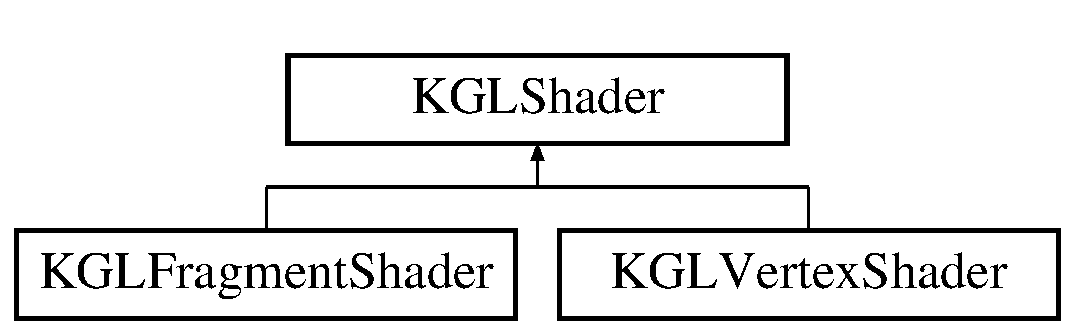
\includegraphics[height=2cm]{class_k_g_l_shader}
\end{center}
\end{figure}
\subsection*{Public Member Functions}
\begin{CompactItemize}
\item 
\hyperlink{class_k_g_l_shader_d248b6b4159c8ef1c421f64f15f3a2bf}{KGLShader} (GLenum type)
\item 
\hyperlink{class_k_g_l_shader_a314186b1c41653d6418c9cbcc673ca7}{KGLShader} (GLenum type, const QString \&filename)
\item 
virtual \hyperlink{class_k_g_l_shader_bec62fc31823215df69160d442944bfc}{$\sim$KGLShader} ()
\item 
void \hyperlink{class_k_g_l_shader_053304f7caa6280d1485f4c89ef2d76f}{setSource} (const QString \&source)
\item 
void \hyperlink{class_k_g_l_shader_a76416255c6cb080de7a92a553129bb9}{setSource} (const QByteArray \&source)
\item 
bool \hyperlink{class_k_g_l_shader_4ab00f3c14eac360fa989209831bc157}{compile} ()
\item 
bool \hyperlink{class_k_g_l_shader_62c2bb3789a5baaa28cd68167e973728}{isValid} () const 
\item 
bool \hyperlink{class_k_g_l_shader_490ad591f21b032aa59ab5c12813f7e8}{isCompiled} () const 
\item 
char $\ast$ \hyperlink{class_k_g_l_shader_f42dca3d4d145a34ea2c2382699a2f19}{compileLog} () const 
\item 
GLenum \hyperlink{class_k_g_l_shader_c059d873e4ed8c305373818da8caf9f2}{type} () const 
\item 
GLuint \hyperlink{class_k_g_l_shader_4a54ab05e1fa2255370fe0145548f0ac}{glId} () const 
\end{CompactItemize}
\subsection*{Protected Member Functions}
\begin{CompactItemize}
\item 
void \hyperlink{class_k_g_l_shader_2c30a1d2be6fb5f4bcae597943cd71d2}{init} (GLenum type)
\end{CompactItemize}
\subsection*{Protected Attributes}
\begin{CompactItemize}
\item 
GLuint \hyperlink{class_k_g_l_shader_3d77624fd6e45291229504184035a02f}{mGLId}
\item 
GLenum \hyperlink{class_k_g_l_shader_9a748dadd159cb1982f37bb8df05ca57}{mType}
\item 
bool \hyperlink{class_k_g_l_shader_1b47e047354eeaab585f99217a509cff}{mValid}
\item 
bool \hyperlink{class_k_g_l_shader_393f2afe8e1d5bb528e3b0dfebdeec94}{mCompiled}
\item 
char $\ast$ \hyperlink{class_k_g_l_shader_f17a1dcd4b5b44e3a6acbfa5d2397c51}{mCompileLog}
\end{CompactItemize}


\subsection{Detailed Description}
Shader class. 

Encapsulates a shader object. Note that shaders are only intermediate objects used to create Program objects. For simple use cases, you can use Program class which can automatically create and use necessary Shader objects.

\begin{Desc}
\item[See also:]Program \end{Desc}


\subsection{Constructor \& Destructor Documentation}
\hypertarget{class_k_g_l_shader_d248b6b4159c8ef1c421f64f15f3a2bf}{
\index{KGLShader@{KGLShader}!KGLShader@{KGLShader}}
\index{KGLShader@{KGLShader}!KGLShader@{KGLShader}}
\subsubsection[{KGLShader}]{\setlength{\rightskip}{0pt plus 5cm}KGLShader::KGLShader (GLenum {\em type})}}
\label{class_k_g_l_shader_d248b6b4159c8ef1c421f64f15f3a2bf}


Creates a shader of given type. You need to manually call \hyperlink{class_k_g_l_shader_053304f7caa6280d1485f4c89ef2d76f}{setSource()} and \hyperlink{class_k_g_l_shader_4ab00f3c14eac360fa989209831bc157}{compile()} before the shader can be added to a Program. \hypertarget{class_k_g_l_shader_a314186b1c41653d6418c9cbcc673ca7}{
\index{KGLShader@{KGLShader}!KGLShader@{KGLShader}}
\index{KGLShader@{KGLShader}!KGLShader@{KGLShader}}
\subsubsection[{KGLShader}]{\setlength{\rightskip}{0pt plus 5cm}KGLShader::KGLShader (GLenum {\em type}, \/  const QString \& {\em filename})}}
\label{class_k_g_l_shader_a314186b1c41653d6418c9cbcc673ca7}


Loads shader of given type from given file. Loaded shader is automatically compiled, so if the compilation succeeds, you can add it to a Program object. \hypertarget{class_k_g_l_shader_bec62fc31823215df69160d442944bfc}{
\index{KGLShader@{KGLShader}!$\sim$KGLShader@{$\sim$KGLShader}}
\index{$\sim$KGLShader@{$\sim$KGLShader}!KGLShader@{KGLShader}}
\subsubsection[{$\sim$KGLShader}]{\setlength{\rightskip}{0pt plus 5cm}KGLShader::$\sim$KGLShader ()\hspace{0.3cm}{\tt  \mbox{[}virtual\mbox{]}}}}
\label{class_k_g_l_shader_bec62fc31823215df69160d442944bfc}


Deletes a shader. Shaders can be deleted after they are added to a Program and the program is linked. 

\subsection{Member Function Documentation}
\hypertarget{class_k_g_l_shader_4ab00f3c14eac360fa989209831bc157}{
\index{KGLShader@{KGLShader}!compile@{compile}}
\index{compile@{compile}!KGLShader@{KGLShader}}
\subsubsection[{compile}]{\setlength{\rightskip}{0pt plus 5cm}bool KGLShader::compile ()}}
\label{class_k_g_l_shader_4ab00f3c14eac360fa989209831bc157}


Compiles the shader. If compilation succeeds, you can add it to a Program object. If compilation fails, you can see the error using \hyperlink{class_k_g_l_shader_f42dca3d4d145a34ea2c2382699a2f19}{compileLog()} method. \hypertarget{class_k_g_l_shader_f42dca3d4d145a34ea2c2382699a2f19}{
\index{KGLShader@{KGLShader}!compileLog@{compileLog}}
\index{compileLog@{compileLog}!KGLShader@{KGLShader}}
\subsubsection[{compileLog}]{\setlength{\rightskip}{0pt plus 5cm}char$\ast$ KGLShader::compileLog () const\hspace{0.3cm}{\tt  \mbox{[}inline\mbox{]}}}}
\label{class_k_g_l_shader_f42dca3d4d145a34ea2c2382699a2f19}


\begin{Desc}
\item[Returns:]Compile log of the shader or null if there was none or the shader hasn't been compiled. Note that Shader keeps ownership of the returned string, so you mustn't delete it. TODO: maybe return QString? \end{Desc}
\hypertarget{class_k_g_l_shader_4a54ab05e1fa2255370fe0145548f0ac}{
\index{KGLShader@{KGLShader}!glId@{glId}}
\index{glId@{glId}!KGLShader@{KGLShader}}
\subsubsection[{glId}]{\setlength{\rightskip}{0pt plus 5cm}GLuint KGLShader::glId () const\hspace{0.3cm}{\tt  \mbox{[}inline\mbox{]}}}}
\label{class_k_g_l_shader_4a54ab05e1fa2255370fe0145548f0ac}


\hypertarget{class_k_g_l_shader_2c30a1d2be6fb5f4bcae597943cd71d2}{
\index{KGLShader@{KGLShader}!init@{init}}
\index{init@{init}!KGLShader@{KGLShader}}
\subsubsection[{init}]{\setlength{\rightskip}{0pt plus 5cm}void KGLShader::init (GLenum {\em type})\hspace{0.3cm}{\tt  \mbox{[}protected\mbox{]}}}}
\label{class_k_g_l_shader_2c30a1d2be6fb5f4bcae597943cd71d2}


\hypertarget{class_k_g_l_shader_490ad591f21b032aa59ab5c12813f7e8}{
\index{KGLShader@{KGLShader}!isCompiled@{isCompiled}}
\index{isCompiled@{isCompiled}!KGLShader@{KGLShader}}
\subsubsection[{isCompiled}]{\setlength{\rightskip}{0pt plus 5cm}bool KGLShader::isCompiled () const\hspace{0.3cm}{\tt  \mbox{[}inline\mbox{]}}}}
\label{class_k_g_l_shader_490ad591f21b032aa59ab5c12813f7e8}


\hypertarget{class_k_g_l_shader_62c2bb3789a5baaa28cd68167e973728}{
\index{KGLShader@{KGLShader}!isValid@{isValid}}
\index{isValid@{isValid}!KGLShader@{KGLShader}}
\subsubsection[{isValid}]{\setlength{\rightskip}{0pt plus 5cm}bool KGLShader::isValid () const\hspace{0.3cm}{\tt  \mbox{[}inline\mbox{]}}}}
\label{class_k_g_l_shader_62c2bb3789a5baaa28cd68167e973728}


\hypertarget{class_k_g_l_shader_a76416255c6cb080de7a92a553129bb9}{
\index{KGLShader@{KGLShader}!setSource@{setSource}}
\index{setSource@{setSource}!KGLShader@{KGLShader}}
\subsubsection[{setSource}]{\setlength{\rightskip}{0pt plus 5cm}void KGLShader::setSource (const QByteArray \& {\em source})}}
\label{class_k_g_l_shader_a76416255c6cb080de7a92a553129bb9}


\hypertarget{class_k_g_l_shader_053304f7caa6280d1485f4c89ef2d76f}{
\index{KGLShader@{KGLShader}!setSource@{setSource}}
\index{setSource@{setSource}!KGLShader@{KGLShader}}
\subsubsection[{setSource}]{\setlength{\rightskip}{0pt plus 5cm}void KGLShader::setSource (const QString \& {\em source})}}
\label{class_k_g_l_shader_053304f7caa6280d1485f4c89ef2d76f}


Sets shader source to {\tt source}. Next you will need to compile the shader. \hypertarget{class_k_g_l_shader_c059d873e4ed8c305373818da8caf9f2}{
\index{KGLShader@{KGLShader}!type@{type}}
\index{type@{type}!KGLShader@{KGLShader}}
\subsubsection[{type}]{\setlength{\rightskip}{0pt plus 5cm}GLenum KGLShader::type () const\hspace{0.3cm}{\tt  \mbox{[}inline\mbox{]}}}}
\label{class_k_g_l_shader_c059d873e4ed8c305373818da8caf9f2}




\subsection{Member Data Documentation}
\hypertarget{class_k_g_l_shader_393f2afe8e1d5bb528e3b0dfebdeec94}{
\index{KGLShader@{KGLShader}!mCompiled@{mCompiled}}
\index{mCompiled@{mCompiled}!KGLShader@{KGLShader}}
\subsubsection[{mCompiled}]{\setlength{\rightskip}{0pt plus 5cm}bool {\bf KGLShader::mCompiled}\hspace{0.3cm}{\tt  \mbox{[}protected\mbox{]}}}}
\label{class_k_g_l_shader_393f2afe8e1d5bb528e3b0dfebdeec94}


\hypertarget{class_k_g_l_shader_f17a1dcd4b5b44e3a6acbfa5d2397c51}{
\index{KGLShader@{KGLShader}!mCompileLog@{mCompileLog}}
\index{mCompileLog@{mCompileLog}!KGLShader@{KGLShader}}
\subsubsection[{mCompileLog}]{\setlength{\rightskip}{0pt plus 5cm}char$\ast$ {\bf KGLShader::mCompileLog}\hspace{0.3cm}{\tt  \mbox{[}protected\mbox{]}}}}
\label{class_k_g_l_shader_f17a1dcd4b5b44e3a6acbfa5d2397c51}


\hypertarget{class_k_g_l_shader_3d77624fd6e45291229504184035a02f}{
\index{KGLShader@{KGLShader}!mGLId@{mGLId}}
\index{mGLId@{mGLId}!KGLShader@{KGLShader}}
\subsubsection[{mGLId}]{\setlength{\rightskip}{0pt plus 5cm}GLuint {\bf KGLShader::mGLId}\hspace{0.3cm}{\tt  \mbox{[}protected\mbox{]}}}}
\label{class_k_g_l_shader_3d77624fd6e45291229504184035a02f}


\hypertarget{class_k_g_l_shader_9a748dadd159cb1982f37bb8df05ca57}{
\index{KGLShader@{KGLShader}!mType@{mType}}
\index{mType@{mType}!KGLShader@{KGLShader}}
\subsubsection[{mType}]{\setlength{\rightskip}{0pt plus 5cm}GLenum {\bf KGLShader::mType}\hspace{0.3cm}{\tt  \mbox{[}protected\mbox{]}}}}
\label{class_k_g_l_shader_9a748dadd159cb1982f37bb8df05ca57}


\hypertarget{class_k_g_l_shader_1b47e047354eeaab585f99217a509cff}{
\index{KGLShader@{KGLShader}!mValid@{mValid}}
\index{mValid@{mValid}!KGLShader@{KGLShader}}
\subsubsection[{mValid}]{\setlength{\rightskip}{0pt plus 5cm}bool {\bf KGLShader::mValid}\hspace{0.3cm}{\tt  \mbox{[}protected\mbox{]}}}}
\label{class_k_g_l_shader_1b47e047354eeaab585f99217a509cff}




The documentation for this class was generated from the following files:\begin{CompactItemize}
\item 
/home/sacha/programmation/gluon/kgl/\hyperlink{kglshader_8h}{kglshader.h}\item 
/home/sacha/programmation/gluon/kgl/\hyperlink{kglshader_8cpp}{kglshader.cpp}\end{CompactItemize}

\hypertarget{class_k_g_l_shadow_item}{
\section{KGLShadowItem Class Reference}
\label{class_k_g_l_shadow_item}\index{KGLShadowItem@{KGLShadowItem}}
}
{\tt \#include $<$kglshadowitem.h$>$}

Inheritance diagram for KGLShadowItem::\begin{figure}[H]
\begin{center}
\leavevmode
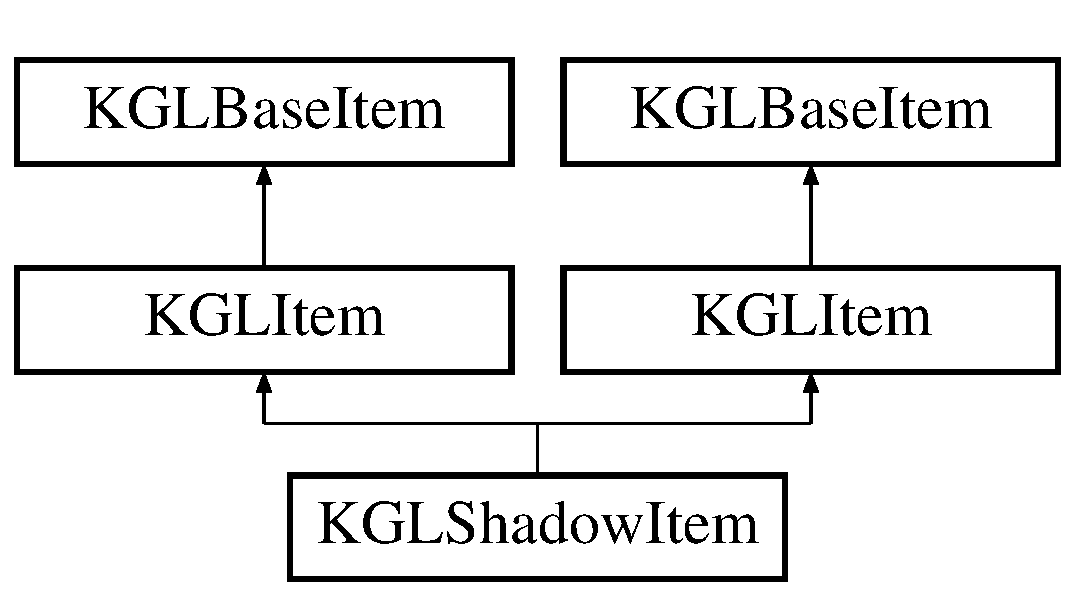
\includegraphics[height=3cm]{class_k_g_l_shadow_item}
\end{center}
\end{figure}
\subsection*{Public Slots}
\begin{CompactItemize}
\item 
void \hyperlink{class_k_g_l_shadow_item_e597951a632787a9f9ada111a051db8a}{snapMatrix} ()
\item 
void \hyperlink{class_k_g_l_shadow_item_936437c9a0cf323cb580e0697fd10b6e}{enable} (bool t=1)
\item 
void \hyperlink{class_k_g_l_shadow_item_97433b863559d8f38199fe68a5b21bcc}{draw} ()
\item 
void \hyperlink{class_k_g_l_shadow_item_0aa1f4701dc69f8b4972d9a5e6b22e1e}{setSnapDuration} (float d)
\item 
void \hyperlink{class_k_g_l_shadow_item_b337d40ec80798586d13a96d648c5b6c}{setNbFrame} (float d)
\item 
void \hyperlink{class_k_g_l_shadow_item_e597951a632787a9f9ada111a051db8a}{snapMatrix} ()
\item 
void \hyperlink{class_k_g_l_shadow_item_936437c9a0cf323cb580e0697fd10b6e}{enable} (bool t=1)
\item 
void \hyperlink{class_k_g_l_shadow_item_97433b863559d8f38199fe68a5b21bcc}{draw} ()
\item 
void \hyperlink{class_k_g_l_shadow_item_0aa1f4701dc69f8b4972d9a5e6b22e1e}{setSnapDuration} (float d)
\item 
void \hyperlink{class_k_g_l_shadow_item_b337d40ec80798586d13a96d648c5b6c}{setNbFrame} (float d)
\end{CompactItemize}
\subsection*{Public Member Functions}
\begin{CompactItemize}
\item 
\hyperlink{class_k_g_l_shadow_item_71f37660873e0f5c56e8c079bebf0184}{KGLShadowItem} (KGLItemBase $\ast$item=0)
\item 
\hyperlink{class_k_g_l_shadow_item_52005ae1bd9e74b02cfb1212a7d5d06b}{KGLShadowItem} (\hyperlink{class_k_g_l_item}{KGLItem} $\ast$item=0)
\end{CompactItemize}


\subsection{Constructor \& Destructor Documentation}
\hypertarget{class_k_g_l_shadow_item_71f37660873e0f5c56e8c079bebf0184}{
\index{KGLShadowItem@{KGLShadowItem}!KGLShadowItem@{KGLShadowItem}}
\index{KGLShadowItem@{KGLShadowItem}!KGLShadowItem@{KGLShadowItem}}
\subsubsection[{KGLShadowItem}]{\setlength{\rightskip}{0pt plus 5cm}KGLShadowItem::KGLShadowItem (KGLItemBase $\ast$ {\em item} = {\tt 0})}}
\label{class_k_g_l_shadow_item_71f37660873e0f5c56e8c079bebf0184}


\hypertarget{class_k_g_l_shadow_item_52005ae1bd9e74b02cfb1212a7d5d06b}{
\index{KGLShadowItem@{KGLShadowItem}!KGLShadowItem@{KGLShadowItem}}
\index{KGLShadowItem@{KGLShadowItem}!KGLShadowItem@{KGLShadowItem}}
\subsubsection[{KGLShadowItem}]{\setlength{\rightskip}{0pt plus 5cm}KGLShadowItem::KGLShadowItem ({\bf KGLItem} $\ast$ {\em item} = {\tt 0})}}
\label{class_k_g_l_shadow_item_52005ae1bd9e74b02cfb1212a7d5d06b}




\subsection{Member Function Documentation}
\hypertarget{class_k_g_l_shadow_item_97433b863559d8f38199fe68a5b21bcc}{
\index{KGLShadowItem@{KGLShadowItem}!draw@{draw}}
\index{draw@{draw}!KGLShadowItem@{KGLShadowItem}}
\subsubsection[{draw}]{\setlength{\rightskip}{0pt plus 5cm}void KGLShadowItem::draw ()\hspace{0.3cm}{\tt  \mbox{[}virtual, slot\mbox{]}}}}
\label{class_k_g_l_shadow_item_97433b863559d8f38199fe68a5b21bcc}




Reimplemented from \hyperlink{class_k_g_l_item_4e4766cf0362fa050bffdf5f45d6d13f}{KGLItem}.\hypertarget{class_k_g_l_shadow_item_97433b863559d8f38199fe68a5b21bcc}{
\index{KGLShadowItem@{KGLShadowItem}!draw@{draw}}
\index{draw@{draw}!KGLShadowItem@{KGLShadowItem}}
\subsubsection[{draw}]{\setlength{\rightskip}{0pt plus 5cm}void KGLShadowItem::draw ()\hspace{0.3cm}{\tt  \mbox{[}virtual, slot\mbox{]}}}}
\label{class_k_g_l_shadow_item_97433b863559d8f38199fe68a5b21bcc}




Reimplemented from \hyperlink{class_k_g_l_item_4e4766cf0362fa050bffdf5f45d6d13f}{KGLItem}.\hypertarget{class_k_g_l_shadow_item_936437c9a0cf323cb580e0697fd10b6e}{
\index{KGLShadowItem@{KGLShadowItem}!enable@{enable}}
\index{enable@{enable}!KGLShadowItem@{KGLShadowItem}}
\subsubsection[{enable}]{\setlength{\rightskip}{0pt plus 5cm}void KGLShadowItem::enable (bool {\em t} = {\tt 1})\hspace{0.3cm}{\tt  \mbox{[}inline, slot\mbox{]}}}}
\label{class_k_g_l_shadow_item_936437c9a0cf323cb580e0697fd10b6e}


\hypertarget{class_k_g_l_shadow_item_936437c9a0cf323cb580e0697fd10b6e}{
\index{KGLShadowItem@{KGLShadowItem}!enable@{enable}}
\index{enable@{enable}!KGLShadowItem@{KGLShadowItem}}
\subsubsection[{enable}]{\setlength{\rightskip}{0pt plus 5cm}void KGLShadowItem::enable (bool {\em t} = {\tt 1})\hspace{0.3cm}{\tt  \mbox{[}inline, slot\mbox{]}}}}
\label{class_k_g_l_shadow_item_936437c9a0cf323cb580e0697fd10b6e}


\hypertarget{class_k_g_l_shadow_item_b337d40ec80798586d13a96d648c5b6c}{
\index{KGLShadowItem@{KGLShadowItem}!setNbFrame@{setNbFrame}}
\index{setNbFrame@{setNbFrame}!KGLShadowItem@{KGLShadowItem}}
\subsubsection[{setNbFrame}]{\setlength{\rightskip}{0pt plus 5cm}void KGLShadowItem::setNbFrame (float {\em d})\hspace{0.3cm}{\tt  \mbox{[}slot\mbox{]}}}}
\label{class_k_g_l_shadow_item_b337d40ec80798586d13a96d648c5b6c}


\hypertarget{class_k_g_l_shadow_item_b337d40ec80798586d13a96d648c5b6c}{
\index{KGLShadowItem@{KGLShadowItem}!setNbFrame@{setNbFrame}}
\index{setNbFrame@{setNbFrame}!KGLShadowItem@{KGLShadowItem}}
\subsubsection[{setNbFrame}]{\setlength{\rightskip}{0pt plus 5cm}void KGLShadowItem::setNbFrame (float {\em d})\hspace{0.3cm}{\tt  \mbox{[}slot\mbox{]}}}}
\label{class_k_g_l_shadow_item_b337d40ec80798586d13a96d648c5b6c}


\hypertarget{class_k_g_l_shadow_item_0aa1f4701dc69f8b4972d9a5e6b22e1e}{
\index{KGLShadowItem@{KGLShadowItem}!setSnapDuration@{setSnapDuration}}
\index{setSnapDuration@{setSnapDuration}!KGLShadowItem@{KGLShadowItem}}
\subsubsection[{setSnapDuration}]{\setlength{\rightskip}{0pt plus 5cm}void KGLShadowItem::setSnapDuration (float {\em d})\hspace{0.3cm}{\tt  \mbox{[}inline, slot\mbox{]}}}}
\label{class_k_g_l_shadow_item_0aa1f4701dc69f8b4972d9a5e6b22e1e}


\hypertarget{class_k_g_l_shadow_item_0aa1f4701dc69f8b4972d9a5e6b22e1e}{
\index{KGLShadowItem@{KGLShadowItem}!setSnapDuration@{setSnapDuration}}
\index{setSnapDuration@{setSnapDuration}!KGLShadowItem@{KGLShadowItem}}
\subsubsection[{setSnapDuration}]{\setlength{\rightskip}{0pt plus 5cm}void KGLShadowItem::setSnapDuration (float {\em d})\hspace{0.3cm}{\tt  \mbox{[}inline, slot\mbox{]}}}}
\label{class_k_g_l_shadow_item_0aa1f4701dc69f8b4972d9a5e6b22e1e}


\hypertarget{class_k_g_l_shadow_item_e597951a632787a9f9ada111a051db8a}{
\index{KGLShadowItem@{KGLShadowItem}!snapMatrix@{snapMatrix}}
\index{snapMatrix@{snapMatrix}!KGLShadowItem@{KGLShadowItem}}
\subsubsection[{snapMatrix}]{\setlength{\rightskip}{0pt plus 5cm}void KGLShadowItem::snapMatrix ()\hspace{0.3cm}{\tt  \mbox{[}slot\mbox{]}}}}
\label{class_k_g_l_shadow_item_e597951a632787a9f9ada111a051db8a}


\hypertarget{class_k_g_l_shadow_item_e597951a632787a9f9ada111a051db8a}{
\index{KGLShadowItem@{KGLShadowItem}!snapMatrix@{snapMatrix}}
\index{snapMatrix@{snapMatrix}!KGLShadowItem@{KGLShadowItem}}
\subsubsection[{snapMatrix}]{\setlength{\rightskip}{0pt plus 5cm}void KGLShadowItem::snapMatrix ()\hspace{0.3cm}{\tt  \mbox{[}slot\mbox{]}}}}
\label{class_k_g_l_shadow_item_e597951a632787a9f9ada111a051db8a}




The documentation for this class was generated from the following files:\begin{CompactItemize}
\item 
/home/sacha/programmation/gluon/kgl/fx/\hyperlink{fx_2kglshadowitem_8h}{kglshadowitem.h}\item 
/home/sacha/programmation/gluon/kgl/\hyperlink{kglshadowitem_8h}{kglshadowitem.h}\item 
/home/sacha/programmation/gluon/kgl/fx/\hyperlink{fx_2kglshadowitem_8cpp}{kglshadowitem.cpp}\item 
/home/sacha/programmation/gluon/kgl/\hyperlink{kglshadowitem_8cpp}{kglshadowitem.cpp}\end{CompactItemize}

\hypertarget{class_k_g_l_text_item}{
\section{KGLTextItem Class Reference}
\label{class_k_g_l_text_item}\index{KGLTextItem@{KGLTextItem}}
}
{\tt \#include $<$KGLTextItem$>$}

Inheritance diagram for KGLTextItem::\begin{figure}[H]
\begin{center}
\leavevmode
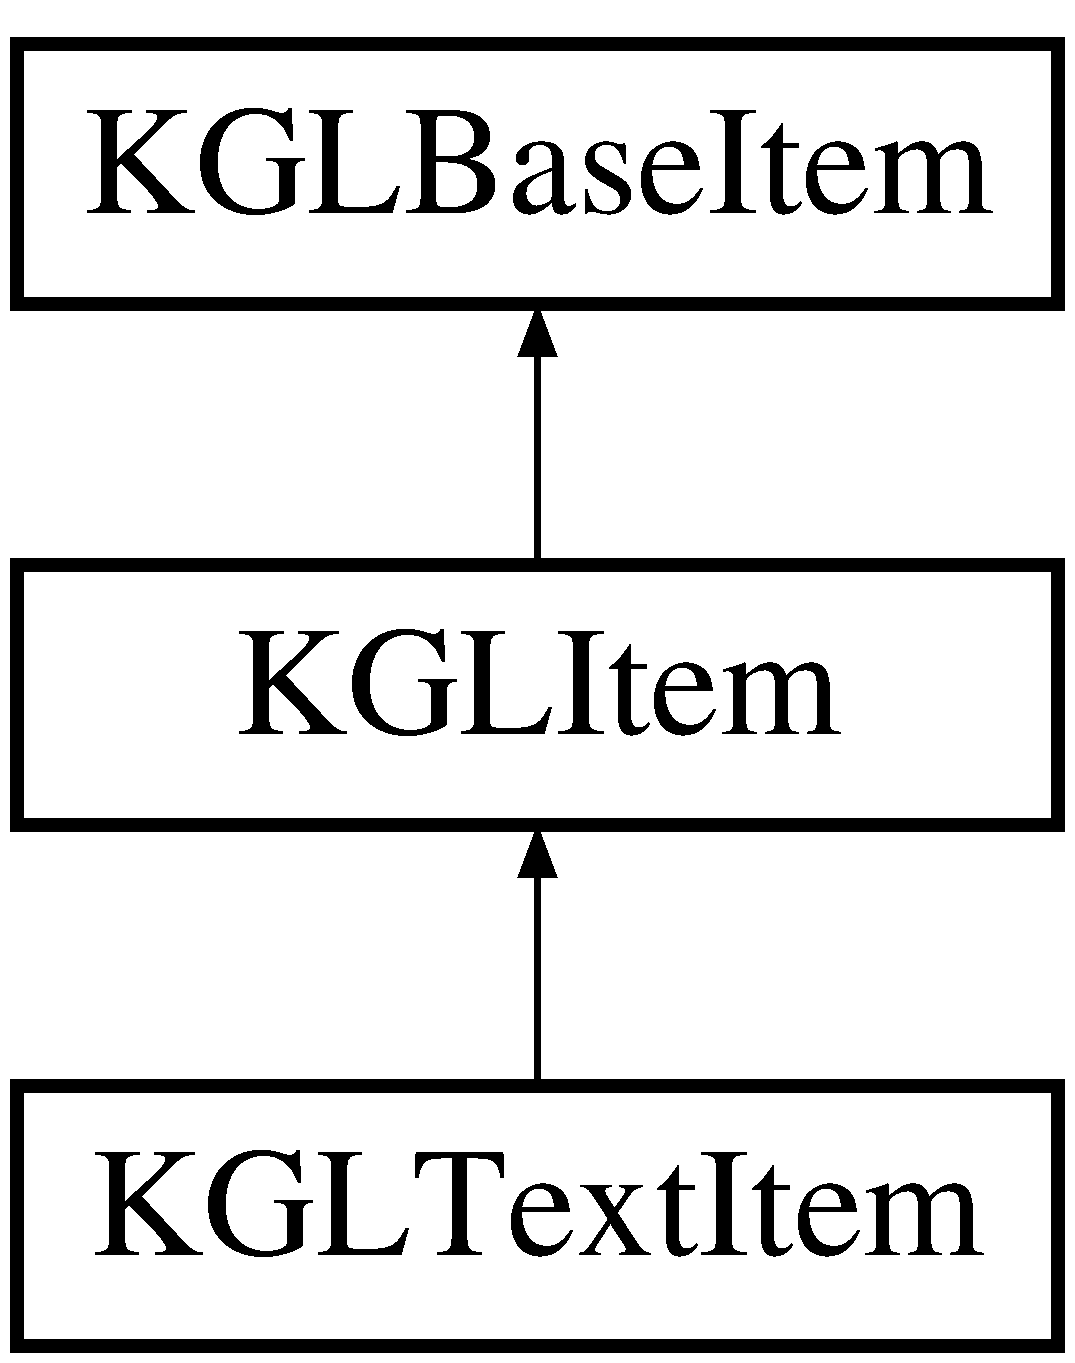
\includegraphics[height=3cm]{class_k_g_l_text_item}
\end{center}
\end{figure}
\subsection*{Public Member Functions}
\begin{CompactItemize}
\item 
\hyperlink{class_k_g_l_text_item_cad71e3ee962c1fdeb5378dc3c4fa0fd}{KGLTextItem} (const QRectF \&rectangle, const QString \&text, \hyperlink{class_k_g_l_engine}{KGLEngine} $\ast$parent=0)
\item 
void \hyperlink{class_k_g_l_text_item_330ab08d8e04a30433439ef60ce82537}{createTexture} ()
\item 
QString \hyperlink{class_k_g_l_text_item_e747fea09561a8d87b464bd304eb8f9c}{text} () const 
\item 
void \hyperlink{class_k_g_l_text_item_7977d97cfd7480c0d5915803e259719c}{setText} (const QString \&text)
\end{CompactItemize}


\subsection{Detailed Description}
This class provides an item that is used to display text. 

\subsection{Constructor \& Destructor Documentation}
\hypertarget{class_k_g_l_text_item_cad71e3ee962c1fdeb5378dc3c4fa0fd}{
\index{KGLTextItem@{KGLTextItem}!KGLTextItem@{KGLTextItem}}
\index{KGLTextItem@{KGLTextItem}!KGLTextItem@{KGLTextItem}}
\subsubsection[{KGLTextItem}]{\setlength{\rightskip}{0pt plus 5cm}KGLTextItem::KGLTextItem (const QRectF \& {\em rectangle}, \/  const QString \& {\em text}, \/  {\bf KGLEngine} $\ast$ {\em parent} = {\tt 0})}}
\label{class_k_g_l_text_item_cad71e3ee962c1fdeb5378dc3c4fa0fd}




\subsection{Member Function Documentation}
\hypertarget{class_k_g_l_text_item_330ab08d8e04a30433439ef60ce82537}{
\index{KGLTextItem@{KGLTextItem}!createTexture@{createTexture}}
\index{createTexture@{createTexture}!KGLTextItem@{KGLTextItem}}
\subsubsection[{createTexture}]{\setlength{\rightskip}{0pt plus 5cm}void KGLTextItem::createTexture ()}}
\label{class_k_g_l_text_item_330ab08d8e04a30433439ef60ce82537}


\hypertarget{class_k_g_l_text_item_7977d97cfd7480c0d5915803e259719c}{
\index{KGLTextItem@{KGLTextItem}!setText@{setText}}
\index{setText@{setText}!KGLTextItem@{KGLTextItem}}
\subsubsection[{setText}]{\setlength{\rightskip}{0pt plus 5cm}void KGLTextItem::setText (const QString \& {\em text})\hspace{0.3cm}{\tt  \mbox{[}inline\mbox{]}}}}
\label{class_k_g_l_text_item_7977d97cfd7480c0d5915803e259719c}


\hypertarget{class_k_g_l_text_item_e747fea09561a8d87b464bd304eb8f9c}{
\index{KGLTextItem@{KGLTextItem}!text@{text}}
\index{text@{text}!KGLTextItem@{KGLTextItem}}
\subsubsection[{text}]{\setlength{\rightskip}{0pt plus 5cm}QString KGLTextItem::text () const\hspace{0.3cm}{\tt  \mbox{[}inline\mbox{]}}}}
\label{class_k_g_l_text_item_e747fea09561a8d87b464bd304eb8f9c}




The documentation for this class was generated from the following files:\begin{CompactItemize}
\item 
/home/sacha/programmation/gluon/kgl/\hyperlink{kgltextitem_8h}{kgltextitem.h}\item 
/home/sacha/programmation/gluon/kgl/\hyperlink{kgltextitem_8cpp}{kgltextitem.cpp}\end{CompactItemize}

\hypertarget{class_k_g_l_texture}{
\section{KGLTexture Class Reference}
\label{class_k_g_l_texture}\index{KGLTexture@{KGLTexture}}
}
{\tt \#include $<$kgltexture.h$>$}

\subsection*{Public Member Functions}
\begin{CompactItemize}
\item 
\hyperlink{class_k_g_l_texture_36b9b3b9bdaeb08e62886b2bf573a41d}{KGLTexture} ()
\item 
\hyperlink{class_k_g_l_texture_c03f57e6b9a2eeefe61011150a4d86ae}{KGLTexture} (const QString \&fileName)
\item 
\hyperlink{class_k_g_l_texture_48c33d3bc28adcc229c8fee5b96c887d}{KGLTexture} (const QImage \&img)
\item 
\hyperlink{class_k_g_l_texture_14a6af5eb6b31f6ce1fad224fdfe828f}{KGLTexture} (const QPixmap \&pix)
\item 
void \hyperlink{class_k_g_l_texture_4f144c01153ec97b0a7e4f457ebe8f06}{setGLTexture} (const GLuint \&t)
\item 
\hyperlink{class_k_g_l_texture_c4b477f122904517bd16cc6d55e9a5e3}{$\sim$KGLTexture} ()
\item 
void \hyperlink{class_k_g_l_texture_ca185912b1f981310404c4be89dd9d52}{bind} ()
\item 
void \hyperlink{class_k_g_l_texture_27e01b57c2af3331eb0295a4ba38bc9c}{unBind} ()
\item 
void \hyperlink{class_k_g_l_texture_7526a64329b83b21af1908860a9f1c0d}{load} (const QImage \&img, int width=0, int height=0)
\item 
GLuint \hyperlink{class_k_g_l_texture_f6699b639b1c5b5c8ba71040961a1ac3}{gltexture} ()
\item 
QImage \hyperlink{class_k_g_l_texture_d8819075431c2c07c4e606565a072a8d}{getQImage} ()
\item 
QSizeF \hyperlink{class_k_g_l_texture_0ce53b8e563c610c0611c7635f885049}{dim} ()
\item 
void \hyperlink{class_k_g_l_texture_7af343304d1b4abf0409e79486aeaa28}{setTranslate} (QPointF t)
\item 
void \hyperlink{class_k_g_l_texture_80402ae0c478ae9186747fb6f7b1a0b0}{setRotate} (float r)
\item 
void \hyperlink{class_k_g_l_texture_dc79d610ddba188a39f4072e8ab9d274}{setScale} (QPointF s)
\item 
void \hyperlink{class_k_g_l_texture_10abdae695fa96ced2ea46a873c6f058}{translate} (QPointF t)
\item 
void \hyperlink{class_k_g_l_texture_638e961fda83c028eb6b9295d1298fdc}{rotate} (float r)
\item 
void \hyperlink{class_k_g_l_texture_4a7059c7c0001c7d758b9bbb91d71525}{scale} (QPointF s)
\item 
void \hyperlink{class_k_g_l_texture_67cf0613953a0d7949e85f39c30d2594}{updateTransform} ()
\end{CompactItemize}
\subsection*{Protected Member Functions}
\begin{CompactItemize}
\item 
void \hyperlink{class_k_g_l_texture_8ce2976f7a178e059436696412b58d24}{init} ()
\end{CompactItemize}


\subsection{Constructor \& Destructor Documentation}
\hypertarget{class_k_g_l_texture_36b9b3b9bdaeb08e62886b2bf573a41d}{
\index{KGLTexture@{KGLTexture}!KGLTexture@{KGLTexture}}
\index{KGLTexture@{KGLTexture}!KGLTexture@{KGLTexture}}
\subsubsection[{KGLTexture}]{\setlength{\rightskip}{0pt plus 5cm}KGLTexture::KGLTexture ()}}
\label{class_k_g_l_texture_36b9b3b9bdaeb08e62886b2bf573a41d}


\hypertarget{class_k_g_l_texture_c03f57e6b9a2eeefe61011150a4d86ae}{
\index{KGLTexture@{KGLTexture}!KGLTexture@{KGLTexture}}
\index{KGLTexture@{KGLTexture}!KGLTexture@{KGLTexture}}
\subsubsection[{KGLTexture}]{\setlength{\rightskip}{0pt plus 5cm}KGLTexture::KGLTexture (const QString \& {\em fileName})}}
\label{class_k_g_l_texture_c03f57e6b9a2eeefe61011150a4d86ae}


\hypertarget{class_k_g_l_texture_48c33d3bc28adcc229c8fee5b96c887d}{
\index{KGLTexture@{KGLTexture}!KGLTexture@{KGLTexture}}
\index{KGLTexture@{KGLTexture}!KGLTexture@{KGLTexture}}
\subsubsection[{KGLTexture}]{\setlength{\rightskip}{0pt plus 5cm}KGLTexture::KGLTexture (const QImage \& {\em img})}}
\label{class_k_g_l_texture_48c33d3bc28adcc229c8fee5b96c887d}


\hypertarget{class_k_g_l_texture_14a6af5eb6b31f6ce1fad224fdfe828f}{
\index{KGLTexture@{KGLTexture}!KGLTexture@{KGLTexture}}
\index{KGLTexture@{KGLTexture}!KGLTexture@{KGLTexture}}
\subsubsection[{KGLTexture}]{\setlength{\rightskip}{0pt plus 5cm}KGLTexture::KGLTexture (const QPixmap \& {\em pix})}}
\label{class_k_g_l_texture_14a6af5eb6b31f6ce1fad224fdfe828f}


\hypertarget{class_k_g_l_texture_c4b477f122904517bd16cc6d55e9a5e3}{
\index{KGLTexture@{KGLTexture}!$\sim$KGLTexture@{$\sim$KGLTexture}}
\index{$\sim$KGLTexture@{$\sim$KGLTexture}!KGLTexture@{KGLTexture}}
\subsubsection[{$\sim$KGLTexture}]{\setlength{\rightskip}{0pt plus 5cm}KGLTexture::$\sim$KGLTexture ()}}
\label{class_k_g_l_texture_c4b477f122904517bd16cc6d55e9a5e3}




\subsection{Member Function Documentation}
\hypertarget{class_k_g_l_texture_ca185912b1f981310404c4be89dd9d52}{
\index{KGLTexture@{KGLTexture}!bind@{bind}}
\index{bind@{bind}!KGLTexture@{KGLTexture}}
\subsubsection[{bind}]{\setlength{\rightskip}{0pt plus 5cm}void KGLTexture::bind ()}}
\label{class_k_g_l_texture_ca185912b1f981310404c4be89dd9d52}


\hypertarget{class_k_g_l_texture_0ce53b8e563c610c0611c7635f885049}{
\index{KGLTexture@{KGLTexture}!dim@{dim}}
\index{dim@{dim}!KGLTexture@{KGLTexture}}
\subsubsection[{dim}]{\setlength{\rightskip}{0pt plus 5cm}QSizeF KGLTexture::dim ()\hspace{0.3cm}{\tt  \mbox{[}inline\mbox{]}}}}
\label{class_k_g_l_texture_0ce53b8e563c610c0611c7635f885049}


\hypertarget{class_k_g_l_texture_d8819075431c2c07c4e606565a072a8d}{
\index{KGLTexture@{KGLTexture}!getQImage@{getQImage}}
\index{getQImage@{getQImage}!KGLTexture@{KGLTexture}}
\subsubsection[{getQImage}]{\setlength{\rightskip}{0pt plus 5cm}QImage KGLTexture::getQImage ()\hspace{0.3cm}{\tt  \mbox{[}inline\mbox{]}}}}
\label{class_k_g_l_texture_d8819075431c2c07c4e606565a072a8d}


\hypertarget{class_k_g_l_texture_f6699b639b1c5b5c8ba71040961a1ac3}{
\index{KGLTexture@{KGLTexture}!gltexture@{gltexture}}
\index{gltexture@{gltexture}!KGLTexture@{KGLTexture}}
\subsubsection[{gltexture}]{\setlength{\rightskip}{0pt plus 5cm}GLuint KGLTexture::gltexture ()\hspace{0.3cm}{\tt  \mbox{[}inline\mbox{]}}}}
\label{class_k_g_l_texture_f6699b639b1c5b5c8ba71040961a1ac3}


\hypertarget{class_k_g_l_texture_8ce2976f7a178e059436696412b58d24}{
\index{KGLTexture@{KGLTexture}!init@{init}}
\index{init@{init}!KGLTexture@{KGLTexture}}
\subsubsection[{init}]{\setlength{\rightskip}{0pt plus 5cm}void KGLTexture::init ()\hspace{0.3cm}{\tt  \mbox{[}protected\mbox{]}}}}
\label{class_k_g_l_texture_8ce2976f7a178e059436696412b58d24}


\hypertarget{class_k_g_l_texture_7526a64329b83b21af1908860a9f1c0d}{
\index{KGLTexture@{KGLTexture}!load@{load}}
\index{load@{load}!KGLTexture@{KGLTexture}}
\subsubsection[{load}]{\setlength{\rightskip}{0pt plus 5cm}void KGLTexture::load (const QImage \& {\em img}, \/  int {\em width} = {\tt 0}, \/  int {\em height} = {\tt 0})}}
\label{class_k_g_l_texture_7526a64329b83b21af1908860a9f1c0d}


\hypertarget{class_k_g_l_texture_638e961fda83c028eb6b9295d1298fdc}{
\index{KGLTexture@{KGLTexture}!rotate@{rotate}}
\index{rotate@{rotate}!KGLTexture@{KGLTexture}}
\subsubsection[{rotate}]{\setlength{\rightskip}{0pt plus 5cm}void KGLTexture::rotate (float {\em r})\hspace{0.3cm}{\tt  \mbox{[}inline\mbox{]}}}}
\label{class_k_g_l_texture_638e961fda83c028eb6b9295d1298fdc}


\hypertarget{class_k_g_l_texture_4a7059c7c0001c7d758b9bbb91d71525}{
\index{KGLTexture@{KGLTexture}!scale@{scale}}
\index{scale@{scale}!KGLTexture@{KGLTexture}}
\subsubsection[{scale}]{\setlength{\rightskip}{0pt plus 5cm}void KGLTexture::scale (QPointF {\em s})\hspace{0.3cm}{\tt  \mbox{[}inline\mbox{]}}}}
\label{class_k_g_l_texture_4a7059c7c0001c7d758b9bbb91d71525}


\hypertarget{class_k_g_l_texture_4f144c01153ec97b0a7e4f457ebe8f06}{
\index{KGLTexture@{KGLTexture}!setGLTexture@{setGLTexture}}
\index{setGLTexture@{setGLTexture}!KGLTexture@{KGLTexture}}
\subsubsection[{setGLTexture}]{\setlength{\rightskip}{0pt plus 5cm}void KGLTexture::setGLTexture (const GLuint \& {\em t})\hspace{0.3cm}{\tt  \mbox{[}inline\mbox{]}}}}
\label{class_k_g_l_texture_4f144c01153ec97b0a7e4f457ebe8f06}


\hypertarget{class_k_g_l_texture_80402ae0c478ae9186747fb6f7b1a0b0}{
\index{KGLTexture@{KGLTexture}!setRotate@{setRotate}}
\index{setRotate@{setRotate}!KGLTexture@{KGLTexture}}
\subsubsection[{setRotate}]{\setlength{\rightskip}{0pt plus 5cm}void KGLTexture::setRotate (float {\em r})\hspace{0.3cm}{\tt  \mbox{[}inline\mbox{]}}}}
\label{class_k_g_l_texture_80402ae0c478ae9186747fb6f7b1a0b0}


\hypertarget{class_k_g_l_texture_dc79d610ddba188a39f4072e8ab9d274}{
\index{KGLTexture@{KGLTexture}!setScale@{setScale}}
\index{setScale@{setScale}!KGLTexture@{KGLTexture}}
\subsubsection[{setScale}]{\setlength{\rightskip}{0pt plus 5cm}void KGLTexture::setScale (QPointF {\em s})\hspace{0.3cm}{\tt  \mbox{[}inline\mbox{]}}}}
\label{class_k_g_l_texture_dc79d610ddba188a39f4072e8ab9d274}


\hypertarget{class_k_g_l_texture_7af343304d1b4abf0409e79486aeaa28}{
\index{KGLTexture@{KGLTexture}!setTranslate@{setTranslate}}
\index{setTranslate@{setTranslate}!KGLTexture@{KGLTexture}}
\subsubsection[{setTranslate}]{\setlength{\rightskip}{0pt plus 5cm}void KGLTexture::setTranslate (QPointF {\em t})\hspace{0.3cm}{\tt  \mbox{[}inline\mbox{]}}}}
\label{class_k_g_l_texture_7af343304d1b4abf0409e79486aeaa28}


\hypertarget{class_k_g_l_texture_10abdae695fa96ced2ea46a873c6f058}{
\index{KGLTexture@{KGLTexture}!translate@{translate}}
\index{translate@{translate}!KGLTexture@{KGLTexture}}
\subsubsection[{translate}]{\setlength{\rightskip}{0pt plus 5cm}void KGLTexture::translate (QPointF {\em t})\hspace{0.3cm}{\tt  \mbox{[}inline\mbox{]}}}}
\label{class_k_g_l_texture_10abdae695fa96ced2ea46a873c6f058}


\hypertarget{class_k_g_l_texture_27e01b57c2af3331eb0295a4ba38bc9c}{
\index{KGLTexture@{KGLTexture}!unBind@{unBind}}
\index{unBind@{unBind}!KGLTexture@{KGLTexture}}
\subsubsection[{unBind}]{\setlength{\rightskip}{0pt plus 5cm}void KGLTexture::unBind ()}}
\label{class_k_g_l_texture_27e01b57c2af3331eb0295a4ba38bc9c}


\hypertarget{class_k_g_l_texture_67cf0613953a0d7949e85f39c30d2594}{
\index{KGLTexture@{KGLTexture}!updateTransform@{updateTransform}}
\index{updateTransform@{updateTransform}!KGLTexture@{KGLTexture}}
\subsubsection[{updateTransform}]{\setlength{\rightskip}{0pt plus 5cm}void KGLTexture::updateTransform ()}}
\label{class_k_g_l_texture_67cf0613953a0d7949e85f39c30d2594}




The documentation for this class was generated from the following files:\begin{CompactItemize}
\item 
/home/sacha/programmation/gluon/kgl/\hyperlink{kgltexture_8h}{kgltexture.h}\item 
/home/sacha/programmation/gluon/kgl/\hyperlink{kgltexture_8cpp}{kgltexture.cpp}\end{CompactItemize}

\hypertarget{class_k_g_l_vertex_shader}{
\section{KGLVertexShader Class Reference}
\label{class_k_g_l_vertex_shader}\index{KGLVertexShader@{KGLVertexShader}}
}
{\tt \#include $<$kglshader.h$>$}

Inheritance diagram for KGLVertexShader::\begin{figure}[H]
\begin{center}
\leavevmode
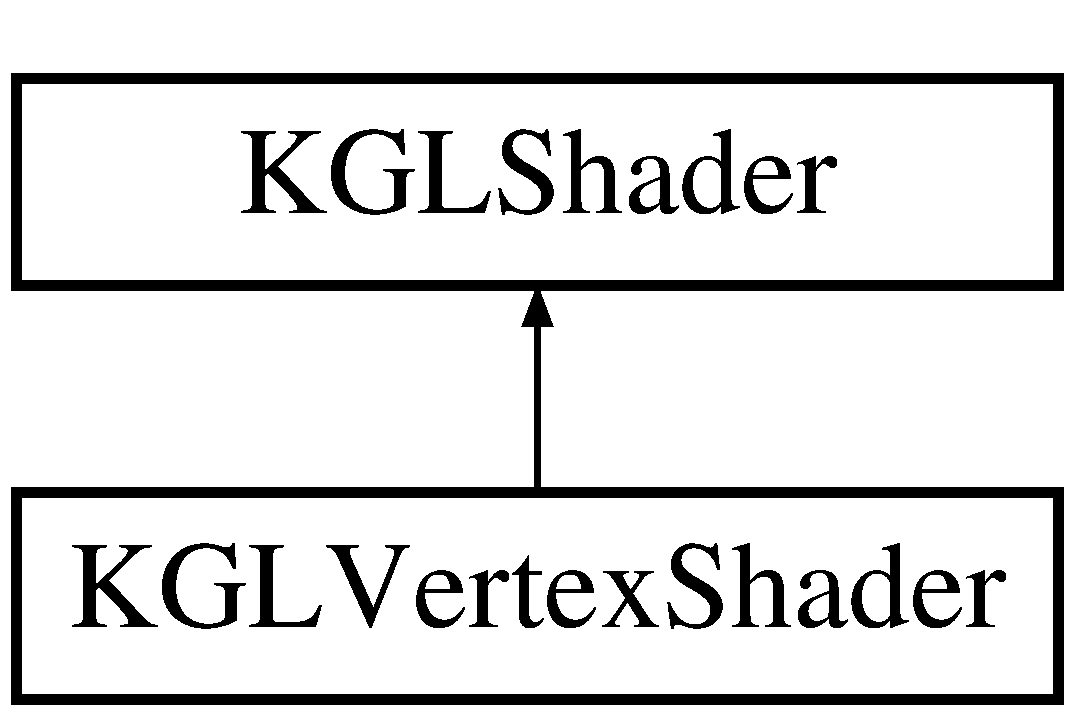
\includegraphics[height=2cm]{class_k_g_l_vertex_shader}
\end{center}
\end{figure}
\subsection*{Public Member Functions}
\begin{CompactItemize}
\item 
\hyperlink{class_k_g_l_vertex_shader_7d4f6727d65757daafbabb4d6b229529}{KGLVertexShader} ()
\item 
\hyperlink{class_k_g_l_vertex_shader_b344fad22cc637f30d0380372fd4a5ec}{KGLVertexShader} (const QString \&filename)
\end{CompactItemize}


\subsection{Detailed Description}
Vertex shader subclass, so you needn't pass the type=GL\_\-VERTEX\_\-SHADER parameter to Shader constructor yourself. 

\subsection{Constructor \& Destructor Documentation}
\hypertarget{class_k_g_l_vertex_shader_7d4f6727d65757daafbabb4d6b229529}{
\index{KGLVertexShader@{KGLVertexShader}!KGLVertexShader@{KGLVertexShader}}
\index{KGLVertexShader@{KGLVertexShader}!KGLVertexShader@{KGLVertexShader}}
\subsubsection[{KGLVertexShader}]{\setlength{\rightskip}{0pt plus 5cm}KGLVertexShader::KGLVertexShader ()}}
\label{class_k_g_l_vertex_shader_7d4f6727d65757daafbabb4d6b229529}


\hypertarget{class_k_g_l_vertex_shader_b344fad22cc637f30d0380372fd4a5ec}{
\index{KGLVertexShader@{KGLVertexShader}!KGLVertexShader@{KGLVertexShader}}
\index{KGLVertexShader@{KGLVertexShader}!KGLVertexShader@{KGLVertexShader}}
\subsubsection[{KGLVertexShader}]{\setlength{\rightskip}{0pt plus 5cm}KGLVertexShader::KGLVertexShader (const QString \& {\em filename})}}
\label{class_k_g_l_vertex_shader_b344fad22cc637f30d0380372fd4a5ec}




The documentation for this class was generated from the following files:\begin{CompactItemize}
\item 
/home/sacha/programmation/gluon/kgl/\hyperlink{kglshader_8h}{kglshader.h}\item 
/home/sacha/programmation/gluon/kgl/\hyperlink{kglshader_8cpp}{kglshader.cpp}\end{CompactItemize}

\hypertarget{class_k_g_l_view}{
\section{KGLView Class Reference}
\label{class_k_g_l_view}\index{KGLView@{KGLView}}
}
{\tt \#include $<$kglview.h$>$}

\subsection*{Public Slots}
\begin{CompactItemize}
\item 
virtual void \hyperlink{class_k_g_l_view_793fefddaec50bf299834893ea4a1f91}{nextFrame} ()
\item 
void \hyperlink{class_k_g_l_view_ca124634504e74e91e9d0a00c485c388}{calculFps} ()
\item 
void \hyperlink{class_k_g_l_view_14ed2a52d8843f27bef96b16d4b44c82}{goFullScreen} ()
\item 
void \hyperlink{class_k_g_l_view_996e019a804dcf51749ea900cc02cb83}{leaveFullScreen} ()
\end{CompactItemize}
\subsection*{Public Member Functions}
\begin{CompactItemize}
\item 
\hyperlink{class_k_g_l_view_8ea742580ef43e3fc2dae57c6c49702b}{KGLView} (QSize size, float frameRate, QWidget $\ast$parent=0)
\item 
\hyperlink{class_k_g_l_view_b9286be5ea42882a1bc74e0d09911e0d}{KGLView} (\hyperlink{class_k_g_l_engine}{KGLEngine} $\ast$engine, QWidget $\ast$parent=0)
\item 
\hyperlink{class_k_g_l_view_986c271786b4615af0e6f49e9de8c58d}{KGLView} (QWidget $\ast$parent=0)
\item 
\hyperlink{class_k_g_l_view_78519d715936803fdec2fad8f1d3c7a3}{$\sim$KGLView} ()
\item 
void \hyperlink{class_k_g_l_view_61cfd521e7544d61d7531b29702f9833}{setEngine} (\hyperlink{class_k_g_l_engine}{KGLEngine} $\ast$engine)
\item 
\hyperlink{class_k_g_l_engine}{KGLEngine} $\ast$ \hyperlink{class_k_g_l_view_e426a41ab8a5565bf7bfd861f05cfb46}{engine} ()
\item 
void \hyperlink{class_k_g_l_view_3efd71e05da0e8ee7410ced9f1061090}{start} ()
\item 
void \hyperlink{class_k_g_l_view_bfe4d0dd939222de9c9d4aa8c091b302}{stop} ()
\item 
void \hyperlink{class_k_g_l_view_65ccc66131b6682f5fce7166cb5a4f53}{setFrameRate} (int f)
\item 
void \hyperlink{class_k_g_l_view_841482c1c522ea0fd6d0cbb7f8515613}{setOrthoView} (QRectF \&rect)
\item 
void \hyperlink{class_k_g_l_view_ffc9ca060284bb6f24f2c415710f7b35}{setOrthoView} (const float \&left, const float \&right, const float \&bottom, const float \&top)
\item 
QPointF \hyperlink{class_k_g_l_view_b5d64f06b3602a0ca6ff41d71fc65aa3}{mapToGL} (const QPointF \&p)
\item 
QPointF \hyperlink{class_k_g_l_view_7afa395fcb499b10cd3303e9dede9cef}{mapFromGL} (const QPointF \&p)
\item 
\hyperlink{class_k_g_l_screen_config}{KGLScreenConfig} $\ast$ \hyperlink{class_k_g_l_view_ead550d304e10d08fdaa06416b53d7cf}{screenConfig} ()
\item 
void \hyperlink{class_k_g_l_view_ec41126c626102bf54b1188714fc4a4f}{setMode} (GLenum mode)
\item 
void \hyperlink{class_k_g_l_view_f8263dcf540805c60d724c50e539075f}{setAxisShow} (bool b)
\item 
bool \hyperlink{class_k_g_l_view_865bf8ed1692292d820f13b2321e799d}{isAxisShow} ()
\item 
void \hyperlink{class_k_g_l_view_f9d4eb0a56f1554b348e346cd2342af3}{setInfoShow} (bool b)
\item 
bool \hyperlink{class_k_g_l_view_369ac3eaa08535c8b333d6b8c3793ea1}{isInfoShow} ()
\item 
bool \hyperlink{class_k_g_l_view_c2cc43b86ba6526450d7e9fa3403a484}{isExtensionSupported} (QString name)
\item 
bool \hyperlink{class_k_g_l_view_c1f4d61a7d289074b048ff5791bb3eb5}{isShaderSupported} ()
\item 
float \hyperlink{class_k_g_l_view_ced2f61bddfddf00dba43091176b60ec}{fps} ()
\item 
void \hyperlink{class_k_g_l_view_90318195b5d7d7b03b8d0f21e1993495}{drawRepere} (float scalex, float scaley)
\item 
void \hyperlink{class_k_g_l_view_ed5b1c5deb70a6fe75698d6bf13de0d5}{drawInfo} ()
\item 
void \hyperlink{class_k_g_l_view_f51f913a1902dbc506e4a070cb3e3058}{drawGLItems} ()
\end{CompactItemize}
\subsection*{Protected Member Functions}
\begin{CompactItemize}
\item 
void \hyperlink{class_k_g_l_view_0f69b4842403e72541e2486ea8d289dd}{saveResolution} ()
\item 
bool \hyperlink{class_k_g_l_view_da553856497a8a6b062c1cdf73a3748e}{initGlew} ()
\item 
void \hyperlink{class_k_g_l_view_50930df9b82dba12bc784823a4b9f1f9}{init} ()
\item 
void \hyperlink{class_k_g_l_view_02a6477b2bd3345fea3a2e55e181475a}{initializeGL} ()
\item 
void \hyperlink{class_k_g_l_view_1599a4d77e626cc204f565031ae5bf81}{resizeGL} (int w, int h)
\item 
void \hyperlink{class_k_g_l_view_46018bb23711a3ae7ce5dc37b46302bb}{paintGL} ()
\end{CompactItemize}


\subsection{Constructor \& Destructor Documentation}
\hypertarget{class_k_g_l_view_8ea742580ef43e3fc2dae57c6c49702b}{
\index{KGLView@{KGLView}!KGLView@{KGLView}}
\index{KGLView@{KGLView}!KGLView@{KGLView}}
\subsubsection[{KGLView}]{\setlength{\rightskip}{0pt plus 5cm}KGLView::KGLView (QSize {\em size}, \/  float {\em frameRate}, \/  QWidget $\ast$ {\em parent} = {\tt 0})\hspace{0.3cm}{\tt  \mbox{[}explicit\mbox{]}}}}
\label{class_k_g_l_view_8ea742580ef43e3fc2dae57c6c49702b}


\hypertarget{class_k_g_l_view_b9286be5ea42882a1bc74e0d09911e0d}{
\index{KGLView@{KGLView}!KGLView@{KGLView}}
\index{KGLView@{KGLView}!KGLView@{KGLView}}
\subsubsection[{KGLView}]{\setlength{\rightskip}{0pt plus 5cm}KGLView::KGLView ({\bf KGLEngine} $\ast$ {\em engine}, \/  QWidget $\ast$ {\em parent} = {\tt 0})\hspace{0.3cm}{\tt  \mbox{[}explicit\mbox{]}}}}
\label{class_k_g_l_view_b9286be5ea42882a1bc74e0d09911e0d}


\hypertarget{class_k_g_l_view_986c271786b4615af0e6f49e9de8c58d}{
\index{KGLView@{KGLView}!KGLView@{KGLView}}
\index{KGLView@{KGLView}!KGLView@{KGLView}}
\subsubsection[{KGLView}]{\setlength{\rightskip}{0pt plus 5cm}KGLView::KGLView (QWidget $\ast$ {\em parent} = {\tt 0})\hspace{0.3cm}{\tt  \mbox{[}explicit\mbox{]}}}}
\label{class_k_g_l_view_986c271786b4615af0e6f49e9de8c58d}


\hypertarget{class_k_g_l_view_78519d715936803fdec2fad8f1d3c7a3}{
\index{KGLView@{KGLView}!$\sim$KGLView@{$\sim$KGLView}}
\index{$\sim$KGLView@{$\sim$KGLView}!KGLView@{KGLView}}
\subsubsection[{$\sim$KGLView}]{\setlength{\rightskip}{0pt plus 5cm}KGLView::$\sim$KGLView ()}}
\label{class_k_g_l_view_78519d715936803fdec2fad8f1d3c7a3}




\subsection{Member Function Documentation}
\hypertarget{class_k_g_l_view_ca124634504e74e91e9d0a00c485c388}{
\index{KGLView@{KGLView}!calculFps@{calculFps}}
\index{calculFps@{calculFps}!KGLView@{KGLView}}
\subsubsection[{calculFps}]{\setlength{\rightskip}{0pt plus 5cm}void KGLView::calculFps ()\hspace{0.3cm}{\tt  \mbox{[}inline, slot\mbox{]}}}}
\label{class_k_g_l_view_ca124634504e74e91e9d0a00c485c388}


\hypertarget{class_k_g_l_view_f51f913a1902dbc506e4a070cb3e3058}{
\index{KGLView@{KGLView}!drawGLItems@{drawGLItems}}
\index{drawGLItems@{drawGLItems}!KGLView@{KGLView}}
\subsubsection[{drawGLItems}]{\setlength{\rightskip}{0pt plus 5cm}void KGLView::drawGLItems ()}}
\label{class_k_g_l_view_f51f913a1902dbc506e4a070cb3e3058}


\hypertarget{class_k_g_l_view_ed5b1c5deb70a6fe75698d6bf13de0d5}{
\index{KGLView@{KGLView}!drawInfo@{drawInfo}}
\index{drawInfo@{drawInfo}!KGLView@{KGLView}}
\subsubsection[{drawInfo}]{\setlength{\rightskip}{0pt plus 5cm}void KGLView::drawInfo ()}}
\label{class_k_g_l_view_ed5b1c5deb70a6fe75698d6bf13de0d5}


\hypertarget{class_k_g_l_view_90318195b5d7d7b03b8d0f21e1993495}{
\index{KGLView@{KGLView}!drawRepere@{drawRepere}}
\index{drawRepere@{drawRepere}!KGLView@{KGLView}}
\subsubsection[{drawRepere}]{\setlength{\rightskip}{0pt plus 5cm}void KGLView::drawRepere (float {\em scalex}, \/  float {\em scaley})}}
\label{class_k_g_l_view_90318195b5d7d7b03b8d0f21e1993495}


\hypertarget{class_k_g_l_view_e426a41ab8a5565bf7bfd861f05cfb46}{
\index{KGLView@{KGLView}!engine@{engine}}
\index{engine@{engine}!KGLView@{KGLView}}
\subsubsection[{engine}]{\setlength{\rightskip}{0pt plus 5cm}{\bf KGLEngine}$\ast$ KGLView::engine ()\hspace{0.3cm}{\tt  \mbox{[}inline\mbox{]}}}}
\label{class_k_g_l_view_e426a41ab8a5565bf7bfd861f05cfb46}


\hypertarget{class_k_g_l_view_ced2f61bddfddf00dba43091176b60ec}{
\index{KGLView@{KGLView}!fps@{fps}}
\index{fps@{fps}!KGLView@{KGLView}}
\subsubsection[{fps}]{\setlength{\rightskip}{0pt plus 5cm}float KGLView::fps ()\hspace{0.3cm}{\tt  \mbox{[}inline\mbox{]}}}}
\label{class_k_g_l_view_ced2f61bddfddf00dba43091176b60ec}


\hypertarget{class_k_g_l_view_14ed2a52d8843f27bef96b16d4b44c82}{
\index{KGLView@{KGLView}!goFullScreen@{goFullScreen}}
\index{goFullScreen@{goFullScreen}!KGLView@{KGLView}}
\subsubsection[{goFullScreen}]{\setlength{\rightskip}{0pt plus 5cm}void KGLView::goFullScreen ()\hspace{0.3cm}{\tt  \mbox{[}slot\mbox{]}}}}
\label{class_k_g_l_view_14ed2a52d8843f27bef96b16d4b44c82}


\hypertarget{class_k_g_l_view_50930df9b82dba12bc784823a4b9f1f9}{
\index{KGLView@{KGLView}!init@{init}}
\index{init@{init}!KGLView@{KGLView}}
\subsubsection[{init}]{\setlength{\rightskip}{0pt plus 5cm}void KGLView::init ()\hspace{0.3cm}{\tt  \mbox{[}protected\mbox{]}}}}
\label{class_k_g_l_view_50930df9b82dba12bc784823a4b9f1f9}


\hypertarget{class_k_g_l_view_da553856497a8a6b062c1cdf73a3748e}{
\index{KGLView@{KGLView}!initGlew@{initGlew}}
\index{initGlew@{initGlew}!KGLView@{KGLView}}
\subsubsection[{initGlew}]{\setlength{\rightskip}{0pt plus 5cm}bool KGLView::initGlew ()\hspace{0.3cm}{\tt  \mbox{[}protected\mbox{]}}}}
\label{class_k_g_l_view_da553856497a8a6b062c1cdf73a3748e}


\hypertarget{class_k_g_l_view_02a6477b2bd3345fea3a2e55e181475a}{
\index{KGLView@{KGLView}!initializeGL@{initializeGL}}
\index{initializeGL@{initializeGL}!KGLView@{KGLView}}
\subsubsection[{initializeGL}]{\setlength{\rightskip}{0pt plus 5cm}void KGLView::initializeGL ()\hspace{0.3cm}{\tt  \mbox{[}protected\mbox{]}}}}
\label{class_k_g_l_view_02a6477b2bd3345fea3a2e55e181475a}


\hypertarget{class_k_g_l_view_865bf8ed1692292d820f13b2321e799d}{
\index{KGLView@{KGLView}!isAxisShow@{isAxisShow}}
\index{isAxisShow@{isAxisShow}!KGLView@{KGLView}}
\subsubsection[{isAxisShow}]{\setlength{\rightskip}{0pt plus 5cm}bool KGLView::isAxisShow ()\hspace{0.3cm}{\tt  \mbox{[}inline\mbox{]}}}}
\label{class_k_g_l_view_865bf8ed1692292d820f13b2321e799d}


\hypertarget{class_k_g_l_view_c2cc43b86ba6526450d7e9fa3403a484}{
\index{KGLView@{KGLView}!isExtensionSupported@{isExtensionSupported}}
\index{isExtensionSupported@{isExtensionSupported}!KGLView@{KGLView}}
\subsubsection[{isExtensionSupported}]{\setlength{\rightskip}{0pt plus 5cm}bool KGLView::isExtensionSupported (QString {\em name})\hspace{0.3cm}{\tt  \mbox{[}inline\mbox{]}}}}
\label{class_k_g_l_view_c2cc43b86ba6526450d7e9fa3403a484}


\hypertarget{class_k_g_l_view_369ac3eaa08535c8b333d6b8c3793ea1}{
\index{KGLView@{KGLView}!isInfoShow@{isInfoShow}}
\index{isInfoShow@{isInfoShow}!KGLView@{KGLView}}
\subsubsection[{isInfoShow}]{\setlength{\rightskip}{0pt plus 5cm}bool KGLView::isInfoShow ()\hspace{0.3cm}{\tt  \mbox{[}inline\mbox{]}}}}
\label{class_k_g_l_view_369ac3eaa08535c8b333d6b8c3793ea1}


\hypertarget{class_k_g_l_view_c1f4d61a7d289074b048ff5791bb3eb5}{
\index{KGLView@{KGLView}!isShaderSupported@{isShaderSupported}}
\index{isShaderSupported@{isShaderSupported}!KGLView@{KGLView}}
\subsubsection[{isShaderSupported}]{\setlength{\rightskip}{0pt plus 5cm}bool KGLView::isShaderSupported ()\hspace{0.3cm}{\tt  \mbox{[}inline\mbox{]}}}}
\label{class_k_g_l_view_c1f4d61a7d289074b048ff5791bb3eb5}


\hypertarget{class_k_g_l_view_996e019a804dcf51749ea900cc02cb83}{
\index{KGLView@{KGLView}!leaveFullScreen@{leaveFullScreen}}
\index{leaveFullScreen@{leaveFullScreen}!KGLView@{KGLView}}
\subsubsection[{leaveFullScreen}]{\setlength{\rightskip}{0pt plus 5cm}void KGLView::leaveFullScreen ()\hspace{0.3cm}{\tt  \mbox{[}inline, slot\mbox{]}}}}
\label{class_k_g_l_view_996e019a804dcf51749ea900cc02cb83}


\hypertarget{class_k_g_l_view_7afa395fcb499b10cd3303e9dede9cef}{
\index{KGLView@{KGLView}!mapFromGL@{mapFromGL}}
\index{mapFromGL@{mapFromGL}!KGLView@{KGLView}}
\subsubsection[{mapFromGL}]{\setlength{\rightskip}{0pt plus 5cm}QPointF KGLView::mapFromGL (const QPointF \& {\em p})\hspace{0.3cm}{\tt  \mbox{[}inline\mbox{]}}}}
\label{class_k_g_l_view_7afa395fcb499b10cd3303e9dede9cef}


\hypertarget{class_k_g_l_view_b5d64f06b3602a0ca6ff41d71fc65aa3}{
\index{KGLView@{KGLView}!mapToGL@{mapToGL}}
\index{mapToGL@{mapToGL}!KGLView@{KGLView}}
\subsubsection[{mapToGL}]{\setlength{\rightskip}{0pt plus 5cm}QPointF KGLView::mapToGL (const QPointF \& {\em p})\hspace{0.3cm}{\tt  \mbox{[}inline\mbox{]}}}}
\label{class_k_g_l_view_b5d64f06b3602a0ca6ff41d71fc65aa3}


\hypertarget{class_k_g_l_view_793fefddaec50bf299834893ea4a1f91}{
\index{KGLView@{KGLView}!nextFrame@{nextFrame}}
\index{nextFrame@{nextFrame}!KGLView@{KGLView}}
\subsubsection[{nextFrame}]{\setlength{\rightskip}{0pt plus 5cm}void KGLView::nextFrame ()\hspace{0.3cm}{\tt  \mbox{[}virtual, slot\mbox{]}}}}
\label{class_k_g_l_view_793fefddaec50bf299834893ea4a1f91}


\hypertarget{class_k_g_l_view_46018bb23711a3ae7ce5dc37b46302bb}{
\index{KGLView@{KGLView}!paintGL@{paintGL}}
\index{paintGL@{paintGL}!KGLView@{KGLView}}
\subsubsection[{paintGL}]{\setlength{\rightskip}{0pt plus 5cm}void KGLView::paintGL ()\hspace{0.3cm}{\tt  \mbox{[}protected\mbox{]}}}}
\label{class_k_g_l_view_46018bb23711a3ae7ce5dc37b46302bb}


\hypertarget{class_k_g_l_view_1599a4d77e626cc204f565031ae5bf81}{
\index{KGLView@{KGLView}!resizeGL@{resizeGL}}
\index{resizeGL@{resizeGL}!KGLView@{KGLView}}
\subsubsection[{resizeGL}]{\setlength{\rightskip}{0pt plus 5cm}void KGLView::resizeGL (int {\em w}, \/  int {\em h})\hspace{0.3cm}{\tt  \mbox{[}protected\mbox{]}}}}
\label{class_k_g_l_view_1599a4d77e626cc204f565031ae5bf81}


\hypertarget{class_k_g_l_view_0f69b4842403e72541e2486ea8d289dd}{
\index{KGLView@{KGLView}!saveResolution@{saveResolution}}
\index{saveResolution@{saveResolution}!KGLView@{KGLView}}
\subsubsection[{saveResolution}]{\setlength{\rightskip}{0pt plus 5cm}void KGLView::saveResolution ()\hspace{0.3cm}{\tt  \mbox{[}protected\mbox{]}}}}
\label{class_k_g_l_view_0f69b4842403e72541e2486ea8d289dd}


\hypertarget{class_k_g_l_view_ead550d304e10d08fdaa06416b53d7cf}{
\index{KGLView@{KGLView}!screenConfig@{screenConfig}}
\index{screenConfig@{screenConfig}!KGLView@{KGLView}}
\subsubsection[{screenConfig}]{\setlength{\rightskip}{0pt plus 5cm}{\bf KGLScreenConfig}$\ast$ KGLView::screenConfig ()\hspace{0.3cm}{\tt  \mbox{[}inline\mbox{]}}}}
\label{class_k_g_l_view_ead550d304e10d08fdaa06416b53d7cf}


\hypertarget{class_k_g_l_view_f8263dcf540805c60d724c50e539075f}{
\index{KGLView@{KGLView}!setAxisShow@{setAxisShow}}
\index{setAxisShow@{setAxisShow}!KGLView@{KGLView}}
\subsubsection[{setAxisShow}]{\setlength{\rightskip}{0pt plus 5cm}void KGLView::setAxisShow (bool {\em b})\hspace{0.3cm}{\tt  \mbox{[}inline\mbox{]}}}}
\label{class_k_g_l_view_f8263dcf540805c60d724c50e539075f}


\hypertarget{class_k_g_l_view_61cfd521e7544d61d7531b29702f9833}{
\index{KGLView@{KGLView}!setEngine@{setEngine}}
\index{setEngine@{setEngine}!KGLView@{KGLView}}
\subsubsection[{setEngine}]{\setlength{\rightskip}{0pt plus 5cm}void KGLView::setEngine ({\bf KGLEngine} $\ast$ {\em engine})\hspace{0.3cm}{\tt  \mbox{[}inline\mbox{]}}}}
\label{class_k_g_l_view_61cfd521e7544d61d7531b29702f9833}


\hypertarget{class_k_g_l_view_65ccc66131b6682f5fce7166cb5a4f53}{
\index{KGLView@{KGLView}!setFrameRate@{setFrameRate}}
\index{setFrameRate@{setFrameRate}!KGLView@{KGLView}}
\subsubsection[{setFrameRate}]{\setlength{\rightskip}{0pt plus 5cm}void KGLView::setFrameRate (int {\em f})\hspace{0.3cm}{\tt  \mbox{[}inline\mbox{]}}}}
\label{class_k_g_l_view_65ccc66131b6682f5fce7166cb5a4f53}


\hypertarget{class_k_g_l_view_f9d4eb0a56f1554b348e346cd2342af3}{
\index{KGLView@{KGLView}!setInfoShow@{setInfoShow}}
\index{setInfoShow@{setInfoShow}!KGLView@{KGLView}}
\subsubsection[{setInfoShow}]{\setlength{\rightskip}{0pt plus 5cm}void KGLView::setInfoShow (bool {\em b})\hspace{0.3cm}{\tt  \mbox{[}inline\mbox{]}}}}
\label{class_k_g_l_view_f9d4eb0a56f1554b348e346cd2342af3}


\hypertarget{class_k_g_l_view_ec41126c626102bf54b1188714fc4a4f}{
\index{KGLView@{KGLView}!setMode@{setMode}}
\index{setMode@{setMode}!KGLView@{KGLView}}
\subsubsection[{setMode}]{\setlength{\rightskip}{0pt plus 5cm}void KGLView::setMode (GLenum {\em mode})\hspace{0.3cm}{\tt  \mbox{[}inline\mbox{]}}}}
\label{class_k_g_l_view_ec41126c626102bf54b1188714fc4a4f}


\hypertarget{class_k_g_l_view_ffc9ca060284bb6f24f2c415710f7b35}{
\index{KGLView@{KGLView}!setOrthoView@{setOrthoView}}
\index{setOrthoView@{setOrthoView}!KGLView@{KGLView}}
\subsubsection[{setOrthoView}]{\setlength{\rightskip}{0pt plus 5cm}void KGLView::setOrthoView (const float \& {\em left}, \/  const float \& {\em right}, \/  const float \& {\em bottom}, \/  const float \& {\em top})\hspace{0.3cm}{\tt  \mbox{[}inline\mbox{]}}}}
\label{class_k_g_l_view_ffc9ca060284bb6f24f2c415710f7b35}


\hypertarget{class_k_g_l_view_841482c1c522ea0fd6d0cbb7f8515613}{
\index{KGLView@{KGLView}!setOrthoView@{setOrthoView}}
\index{setOrthoView@{setOrthoView}!KGLView@{KGLView}}
\subsubsection[{setOrthoView}]{\setlength{\rightskip}{0pt plus 5cm}void KGLView::setOrthoView (QRectF \& {\em rect})\hspace{0.3cm}{\tt  \mbox{[}inline\mbox{]}}}}
\label{class_k_g_l_view_841482c1c522ea0fd6d0cbb7f8515613}


\hypertarget{class_k_g_l_view_3efd71e05da0e8ee7410ced9f1061090}{
\index{KGLView@{KGLView}!start@{start}}
\index{start@{start}!KGLView@{KGLView}}
\subsubsection[{start}]{\setlength{\rightskip}{0pt plus 5cm}void KGLView::start ()\hspace{0.3cm}{\tt  \mbox{[}inline\mbox{]}}}}
\label{class_k_g_l_view_3efd71e05da0e8ee7410ced9f1061090}


\hypertarget{class_k_g_l_view_bfe4d0dd939222de9c9d4aa8c091b302}{
\index{KGLView@{KGLView}!stop@{stop}}
\index{stop@{stop}!KGLView@{KGLView}}
\subsubsection[{stop}]{\setlength{\rightskip}{0pt plus 5cm}void KGLView::stop ()\hspace{0.3cm}{\tt  \mbox{[}inline\mbox{]}}}}
\label{class_k_g_l_view_bfe4d0dd939222de9c9d4aa8c091b302}




The documentation for this class was generated from the following files:\begin{CompactItemize}
\item 
/home/sacha/programmation/gluon/kgl/\hyperlink{kglview_8h}{kglview.h}\item 
/home/sacha/programmation/gluon/kgl/\hyperlink{kglview_8cpp}{kglview.cpp}\end{CompactItemize}

\chapter{File Documentation}
\hypertarget{fx_2kglshadowitem_8cpp}{
\section{/home/sacha/programmation/gluon/kgl/fx/kglshadowitem.cpp File Reference}
\label{fx_2kglshadowitem_8cpp}\index{/home/sacha/programmation/gluon/kgl/fx/kglshadowitem.cpp@{/home/sacha/programmation/gluon/kgl/fx/kglshadowitem.cpp}}
}
{\tt \#include \char`\"{}kglshadowitem.h\char`\"{}}\par
{\tt \#include $<$QDebug$>$}\par

\hypertarget{kglshadowitem_8cpp}{
\section{/home/sacha/programmation/gluon/kgl/kglshadowitem.cpp File Reference}
\label{kglshadowitem_8cpp}\index{/home/sacha/programmation/gluon/kgl/kglshadowitem.cpp@{/home/sacha/programmation/gluon/kgl/kglshadowitem.cpp}}
}
{\tt \#include \char`\"{}kglshadowitem.h\char`\"{}}\par
{\tt \#include $<$QDebug$>$}\par

\hypertarget{fx_2kglshadowitem_8h}{
\section{/home/sacha/programmation/gluon/kgl/fx/kglshadowitem.h File Reference}
\label{fx_2kglshadowitem_8h}\index{/home/sacha/programmation/gluon/kgl/fx/kglshadowitem.h@{/home/sacha/programmation/gluon/kgl/fx/kglshadowitem.h}}
}
{\tt \#include \char`\"{}kglitem.h\char`\"{}}\par
{\tt \#include \char`\"{}kglspriteitem.h\char`\"{}}\par
{\tt \#include $<$Eigen/Geometry$>$}\par
{\tt \#include $<$QtCore/QList$>$}\par
\subsection*{Classes}
\begin{CompactItemize}
\item 
class \hyperlink{class_k_g_l_shadow_item}{KGLShadowItem}
\end{CompactItemize}

\hypertarget{kglshadowitem_8h}{
\section{/home/sacha/programmation/gluon/kgl/kglshadowitem.h File Reference}
\label{kglshadowitem_8h}\index{/home/sacha/programmation/gluon/kgl/kglshadowitem.h@{/home/sacha/programmation/gluon/kgl/kglshadowitem.h}}
}
{\tt \#include \char`\"{}kglitem.h\char`\"{}}\par
{\tt \#include $<$Eigen/Geometry$>$}\par
{\tt \#include $<$QList$>$}\par
{\tt \#include $<$QTimer$>$}\par
\subsection*{Classes}
\begin{CompactItemize}
\item 
class \hyperlink{class_k_g_l_shadow_item}{KGLShadowItem}
\end{CompactItemize}

\hypertarget{kglanimitem_8cpp}{
\section{/home/sacha/programmation/gluon/kgl/kglanimitem.cpp File Reference}
\label{kglanimitem_8cpp}\index{/home/sacha/programmation/gluon/kgl/kglanimitem.cpp@{/home/sacha/programmation/gluon/kgl/kglanimitem.cpp}}
}
{\tt \#include \char`\"{}kglanimitem.h\char`\"{}}\par
{\tt \#include \char`\"{}kglengine2d.h\char`\"{}}\par
{\tt \#include $<$KDebug$>$}\par
{\tt \#include $<$QTimeLine$>$}\par

\hypertarget{kglanimitem_8h}{
\section{/home/sacha/programmation/gluon/kgl/kglanimitem.h File Reference}
\label{kglanimitem_8h}\index{/home/sacha/programmation/gluon/kgl/kglanimitem.h@{/home/sacha/programmation/gluon/kgl/kglanimitem.h}}
}
{\tt \#include \char`\"{}kglitem.h\char`\"{}}\par
\subsection*{Classes}
\begin{CompactItemize}
\item 
class \hyperlink{class_k_g_l_anim_item}{KGLAnimItem}
\end{CompactItemize}

\hypertarget{kglbaseitem_8cpp}{
\section{/home/sacha/programmation/gluon/kgl/kglbaseitem.cpp File Reference}
\label{kglbaseitem_8cpp}\index{/home/sacha/programmation/gluon/kgl/kglbaseitem.cpp@{/home/sacha/programmation/gluon/kgl/kglbaseitem.cpp}}
}
{\tt \#include \char`\"{}kglbaseitem.h\char`\"{}}\par
{\tt \#include $<$algorithm$>$}\par

\hypertarget{kglbaseitem_8h}{
\section{/home/sacha/programmation/gluon/kgl/kglbaseitem.h File Reference}
\label{kglbaseitem_8h}\index{/home/sacha/programmation/gluon/kgl/kglbaseitem.h@{/home/sacha/programmation/gluon/kgl/kglbaseitem.h}}
}
{\tt \#include $<$QObject$>$}\par
{\tt \#include $<$Eigen/Geometry$>$}\par
{\tt \#include $<$QRectF$>$}\par
{\tt \#include $<$QPolygonF$>$}\par
{\tt \#include $<$QTransform$>$}\par
{\tt \#include $<$QSizeF$>$}\par
{\tt \#include $<$QMatrix$>$}\par
{\tt \#include \char`\"{}kglpoint.h\char`\"{}}\par
\subsection*{Classes}
\begin{CompactItemize}
\item 
class \hyperlink{class_k_g_l_base_item}{KGLBaseItem}
\end{CompactItemize}
\subsection*{Functions}
\begin{CompactItemize}
\item 
const Eigen::Vector3d \hyperlink{kglbaseitem_8h_cc3cc019d4abc859354dae4591328283}{AXIS\_\-X} (1, 0, 0)
\item 
const Eigen::Vector3d \hyperlink{kglbaseitem_8h_5f0b852bfd4839bf9de2904a99ccd832}{AXIS\_\-Y} (0, 1, 0)
\item 
const Eigen::Vector3d \hyperlink{kglbaseitem_8h_06ef33c18d7a9c866ce9c2fc6e1b1720}{AXIS\_\-Z} (0, 0, 1)
\end{CompactItemize}


\subsection{Function Documentation}
\hypertarget{kglbaseitem_8h_cc3cc019d4abc859354dae4591328283}{
\index{kglbaseitem.h@{kglbaseitem.h}!AXIS\_\-X@{AXIS\_\-X}}
\index{AXIS\_\-X@{AXIS\_\-X}!kglbaseitem.h@{kglbaseitem.h}}
\subsubsection[{AXIS\_\-X}]{\setlength{\rightskip}{0pt plus 5cm}const Eigen::Vector3d AXIS\_\-X (1, \/  0, \/  0)}}
\label{kglbaseitem_8h_cc3cc019d4abc859354dae4591328283}


\hypertarget{kglbaseitem_8h_5f0b852bfd4839bf9de2904a99ccd832}{
\index{kglbaseitem.h@{kglbaseitem.h}!AXIS\_\-Y@{AXIS\_\-Y}}
\index{AXIS\_\-Y@{AXIS\_\-Y}!kglbaseitem.h@{kglbaseitem.h}}
\subsubsection[{AXIS\_\-Y}]{\setlength{\rightskip}{0pt plus 5cm}const Eigen::Vector3d AXIS\_\-Y (0, \/  1, \/  0)}}
\label{kglbaseitem_8h_5f0b852bfd4839bf9de2904a99ccd832}


\hypertarget{kglbaseitem_8h_06ef33c18d7a9c866ce9c2fc6e1b1720}{
\index{kglbaseitem.h@{kglbaseitem.h}!AXIS\_\-Z@{AXIS\_\-Z}}
\index{AXIS\_\-Z@{AXIS\_\-Z}!kglbaseitem.h@{kglbaseitem.h}}
\subsubsection[{AXIS\_\-Z}]{\setlength{\rightskip}{0pt plus 5cm}const Eigen::Vector3d AXIS\_\-Z (0, \/  0, \/  1)}}
\label{kglbaseitem_8h_06ef33c18d7a9c866ce9c2fc6e1b1720}



\hypertarget{kglboxitem_8cpp}{
\section{/home/sacha/programmation/gluon/kgl/kglboxitem.cpp File Reference}
\label{kglboxitem_8cpp}\index{/home/sacha/programmation/gluon/kgl/kglboxitem.cpp@{/home/sacha/programmation/gluon/kgl/kglboxitem.cpp}}
}
{\tt \#include \char`\"{}kglboxitem.h\char`\"{}}\par

\hypertarget{kglboxitem_8h}{
\section{/home/sacha/programmation/gluon/kgl/kglboxitem.h File Reference}
\label{kglboxitem_8h}\index{/home/sacha/programmation/gluon/kgl/kglboxitem.h@{/home/sacha/programmation/gluon/kgl/kglboxitem.h}}
}
{\tt \#include \char`\"{}kglitem.h\char`\"{}}\par
\subsection*{Classes}
\begin{CompactItemize}
\item 
class \hyperlink{class_k_g_l_box_item}{KGLBoxItem}
\end{CompactItemize}

\hypertarget{kglcircleitem_8cpp}{
\section{/home/sacha/programmation/gluon/kgl/kglcircleitem.cpp File Reference}
\label{kglcircleitem_8cpp}\index{/home/sacha/programmation/gluon/kgl/kglcircleitem.cpp@{/home/sacha/programmation/gluon/kgl/kglcircleitem.cpp}}
}
{\tt \#include \char`\"{}kglcircleitem.h\char`\"{}}\par
{\tt \#include $<$math.h$>$}\par

\hypertarget{kglcircleitem_8h}{
\section{/home/sacha/programmation/gluon/kgl/kglcircleitem.h File Reference}
\label{kglcircleitem_8h}\index{/home/sacha/programmation/gluon/kgl/kglcircleitem.h@{/home/sacha/programmation/gluon/kgl/kglcircleitem.h}}
}
{\tt \#include \char`\"{}kglitem.h\char`\"{}}\par
\subsection*{Classes}
\begin{CompactItemize}
\item 
class \hyperlink{class_k_g_l_circle_item}{KGLCircleItem}
\end{CompactItemize}

\hypertarget{kglcontaineritem_8cpp}{
\section{/home/sacha/programmation/gluon/kgl/kglcontaineritem.cpp File Reference}
\label{kglcontaineritem_8cpp}\index{/home/sacha/programmation/gluon/kgl/kglcontaineritem.cpp@{/home/sacha/programmation/gluon/kgl/kglcontaineritem.cpp}}
}
{\tt \#include \char`\"{}kglcontaineritem.h\char`\"{}}\par

\hypertarget{kglcontaineritem_8h}{
\section{/home/sacha/programmation/gluon/kgl/kglcontaineritem.h File Reference}
\label{kglcontaineritem_8h}\index{/home/sacha/programmation/gluon/kgl/kglcontaineritem.h@{/home/sacha/programmation/gluon/kgl/kglcontaineritem.h}}
}
{\tt \#include \char`\"{}kglitem.h\char`\"{}}\par
{\tt \#include \char`\"{}kglitemlist.h\char`\"{}}\par
{\tt \#include $<$QDataStream$>$}\par
{\tt \#include $<$KDE/KDebug$>$}\par
\subsection*{Classes}
\begin{CompactItemize}
\item 
class \hyperlink{class_k_g_l_container_item}{KGLContainerItem}
\end{CompactItemize}

\hypertarget{kglengine_8cpp}{
\section{/home/sacha/programmation/gluon/kgl/kglengine.cpp File Reference}
\label{kglengine_8cpp}\index{/home/sacha/programmation/gluon/kgl/kglengine.cpp@{/home/sacha/programmation/gluon/kgl/kglengine.cpp}}
}
{\tt \#include \char`\"{}kglengine.h\char`\"{}}\par
{\tt \#include $<$KDebug$>$}\par

\hypertarget{kglengine_8h}{
\section{/home/sacha/programmation/gluon/kgl/kglengine.h File Reference}
\label{kglengine_8h}\index{/home/sacha/programmation/gluon/kgl/kglengine.h@{/home/sacha/programmation/gluon/kgl/kglengine.h}}
}
{\tt \#include $<$QObject$>$}\par
{\tt \#include $<$QMap$>$}\par
{\tt \#include \char`\"{}kglbaseitem.h\char`\"{}}\par
{\tt \#include \char`\"{}kglitemlist.h\char`\"{}}\par
{\tt \#include \char`\"{}kglitem.h\char`\"{}}\par
{\tt \#include \char`\"{}kglboxitem.h\char`\"{}}\par
{\tt \#include \char`\"{}kgltextitem.h\char`\"{}}\par
\subsection*{Classes}
\begin{CompactItemize}
\item 
class \hyperlink{class_k_g_l_engine}{KGLEngine}
\end{CompactItemize}
\subsection*{Typedefs}
\begin{CompactItemize}
\item 
typedef QMap$<$ unsigned int, \hyperlink{class_k_g_l_item_list}{KGLItemList} $>$ \hyperlink{kglengine_8h_b80cbcec260e71c3207c42d7eba43da1}{IndexGroupMap}
\end{CompactItemize}


\subsection{Typedef Documentation}
\hypertarget{kglengine_8h_b80cbcec260e71c3207c42d7eba43da1}{
\index{kglengine.h@{kglengine.h}!IndexGroupMap@{IndexGroupMap}}
\index{IndexGroupMap@{IndexGroupMap}!kglengine.h@{kglengine.h}}
\subsubsection[{IndexGroupMap}]{\setlength{\rightskip}{0pt plus 5cm}typedef QMap$<$unsigned int, {\bf KGLItemList} $>$ {\bf IndexGroupMap}}}
\label{kglengine_8h_b80cbcec260e71c3207c42d7eba43da1}



\hypertarget{kglfullscreen_8cpp}{
\section{/home/sacha/programmation/gluon/kgl/kglfullscreen.cpp File Reference}
\label{kglfullscreen_8cpp}\index{/home/sacha/programmation/gluon/kgl/kglfullscreen.cpp@{/home/sacha/programmation/gluon/kgl/kglfullscreen.cpp}}
}
{\tt \#include \char`\"{}kglscreenconfig.h\char`\"{}}\par

\hypertarget{kglfullscreen_8h}{
\section{/home/sacha/programmation/gluon/kgl/kglfullscreen.h File Reference}
\label{kglfullscreen_8h}\index{/home/sacha/programmation/gluon/kgl/kglfullscreen.h@{/home/sacha/programmation/gluon/kgl/kglfullscreen.h}}
}
{\tt \#include $<$QObject$>$}\par
{\tt \#include $<$QStringList$>$}\par
{\tt \#include $<$X11/Xlib.h$>$}\par
{\tt \#include $<$X11/extensions/Xrandr.h$>$}\par
{\tt \#include $<$QX11Info$>$}\par
\subsection*{Classes}
\begin{CompactItemize}
\item 
class \hyperlink{class_k_g_l_screen_config}{KGLScreenConfig}
\end{CompactItemize}

\hypertarget{kglfx_8cpp}{
\section{/home/sacha/programmation/gluon/kgl/kglfx.cpp File Reference}
\label{kglfx_8cpp}\index{/home/sacha/programmation/gluon/kgl/kglfx.cpp@{/home/sacha/programmation/gluon/kgl/kglfx.cpp}}
}
{\tt \#include \char`\"{}kglfx.h\char`\"{}}\par

\hypertarget{kglfx_8h}{
\section{/home/sacha/programmation/gluon/kgl/kglfx.h File Reference}
\label{kglfx_8h}\index{/home/sacha/programmation/gluon/kgl/kglfx.h@{/home/sacha/programmation/gluon/kgl/kglfx.h}}
}
{\tt \#include \char`\"{}kglprogram.h\char`\"{}}\par
\subsection*{Classes}
\begin{CompactItemize}
\item 
class \hyperlink{class_k_g_l_fx}{KGLFx}
\item 
class \hyperlink{class_k_g_l_light_fx}{KGLLightFx}
\item 
class \hyperlink{class_k_g_l_blur_fx}{KGLBlurFx}
\item 
class \hyperlink{class_k_g_l_pixelate_fx}{KGLPixelateFx}
\end{CompactItemize}

\hypertarget{kglgriditem_8cpp}{
\section{/home/sacha/programmation/gluon/kgl/kglgriditem.cpp File Reference}
\label{kglgriditem_8cpp}\index{/home/sacha/programmation/gluon/kgl/kglgriditem.cpp@{/home/sacha/programmation/gluon/kgl/kglgriditem.cpp}}
}
{\tt \#include \char`\"{}kglgriditem.h\char`\"{}}\par
{\tt \#include $<$KDebug$>$}\par

\hypertarget{kglgriditem_8h}{
\section{/home/sacha/programmation/gluon/kgl/kglgriditem.h File Reference}
\label{kglgriditem_8h}\index{/home/sacha/programmation/gluon/kgl/kglgriditem.h@{/home/sacha/programmation/gluon/kgl/kglgriditem.h}}
}
{\tt \#include \char`\"{}kglitem.h\char`\"{}}\par
{\tt \#include $<$QSizeF$>$}\par
{\tt \#include $<$QList$>$}\par
\subsection*{Classes}
\begin{CompactItemize}
\item 
class \hyperlink{class_k_g_l_grid_item}{KGLGridItem}
\end{CompactItemize}

\hypertarget{kglintro_8cpp}{
\section{/home/sacha/programmation/gluon/kgl/kglintro.cpp File Reference}
\label{kglintro_8cpp}\index{/home/sacha/programmation/gluon/kgl/kglintro.cpp@{/home/sacha/programmation/gluon/kgl/kglintro.cpp}}
}
{\tt \#include \char`\"{}kglintro.h\char`\"{}}\par
{\tt \#include \char`\"{}kglspriteitem.h\char`\"{}}\par
{\tt \#include \char`\"{}kglengine2d.h\char`\"{}}\par
{\tt \#include \char`\"{}textureManaging/kgltexturemanager.h\char`\"{}}\par
{\tt \#include $<$QTimer$>$}\par

\hypertarget{kglintro_8h}{
\section{/home/sacha/programmation/gluon/kgl/kglintro.h File Reference}
\label{kglintro_8h}\index{/home/sacha/programmation/gluon/kgl/kglintro.h@{/home/sacha/programmation/gluon/kgl/kglintro.h}}
}
{\tt \#include \char`\"{}kglcontaineritem.h\char`\"{}}\par
\subsection*{Classes}
\begin{CompactItemize}
\item 
class \hyperlink{class_k_g_l_intro_item}{KGLIntroItem}
\end{CompactItemize}

\hypertarget{kglitem_8cpp}{
\section{/home/sacha/programmation/gluon/kgl/kglitem.cpp File Reference}
\label{kglitem_8cpp}\index{/home/sacha/programmation/gluon/kgl/kglitem.cpp@{/home/sacha/programmation/gluon/kgl/kglitem.cpp}}
}
{\tt \#include \char`\"{}kglitem.h\char`\"{}}\par
{\tt \#include $<$KDebug$>$}\par
{\tt \#include $<$iostream$>$}\par

\hypertarget{kglitem_8h}{
\section{/home/sacha/programmation/gluon/kgl/kglitem.h File Reference}
\label{kglitem_8h}\index{/home/sacha/programmation/gluon/kgl/kglitem.h@{/home/sacha/programmation/gluon/kgl/kglitem.h}}
}
{\tt \#include $<$GL/glew.h$>$}\par
{\tt \#include \char`\"{}kglbaseitem.h\char`\"{}}\par
{\tt \#include \char`\"{}kgltexture.h\char`\"{}}\par
{\tt \#include \char`\"{}kglprogram.h\char`\"{}}\par
\subsection*{Classes}
\begin{CompactItemize}
\item 
class \hyperlink{class_k_g_l_item}{KGLItem}
\end{CompactItemize}

\hypertarget{kglitemlist_8cpp}{
\section{/home/sacha/programmation/gluon/kgl/kglitemlist.cpp File Reference}
\label{kglitemlist_8cpp}\index{/home/sacha/programmation/gluon/kgl/kglitemlist.cpp@{/home/sacha/programmation/gluon/kgl/kglitemlist.cpp}}
}
{\tt \#include \char`\"{}kglitemlist.h\char`\"{}}\par

\hypertarget{kglitemlist_8h}{
\section{/home/sacha/programmation/gluon/kgl/kglitemlist.h File Reference}
\label{kglitemlist_8h}\index{/home/sacha/programmation/gluon/kgl/kglitemlist.h@{/home/sacha/programmation/gluon/kgl/kglitemlist.h}}
}
{\tt \#include $<$QtCore/QList$>$}\par
{\tt \#include \char`\"{}kglitem.h\char`\"{}}\par
\subsection*{Classes}
\begin{CompactItemize}
\item 
class \hyperlink{class_k_g_l_item_list}{KGLItemList}
\end{CompactItemize}

\hypertarget{kglparticlesitem_8cpp}{
\section{/home/sacha/programmation/gluon/kgl/kglparticlesitem.cpp File Reference}
\label{kglparticlesitem_8cpp}\index{/home/sacha/programmation/gluon/kgl/kglparticlesitem.cpp@{/home/sacha/programmation/gluon/kgl/kglparticlesitem.cpp}}
}
{\tt \#include \char`\"{}kglparticlesitem.h\char`\"{}}\par
{\tt \#include $<$KDebug$>$}\par
{\tt \#include $<$QDateTime$>$}\par
{\tt \#include $<$iostream$>$}\par

\hypertarget{kglparticlesitem_8h}{
\section{/home/sacha/programmation/gluon/kgl/kglparticlesitem.h File Reference}
\label{kglparticlesitem_8h}\index{/home/sacha/programmation/gluon/kgl/kglparticlesitem.h@{/home/sacha/programmation/gluon/kgl/kglparticlesitem.h}}
}
{\tt \#include \char`\"{}kgltexture.h\char`\"{}}\par
{\tt \#include \char`\"{}kglitem.h\char`\"{}}\par
\subsection*{Classes}
\begin{CompactItemize}
\item 
class \hyperlink{class_k_g_l_particle}{KGLParticle}
\item 
class \hyperlink{class_k_g_l_particles_item}{KGLParticlesItem}
\end{CompactItemize}

\hypertarget{kglphysicsengine_8cpp}{
\section{/home/sacha/programmation/gluon/kgl/kglphysicsengine.cpp File Reference}
\label{kglphysicsengine_8cpp}\index{/home/sacha/programmation/gluon/kgl/kglphysicsengine.cpp@{/home/sacha/programmation/gluon/kgl/kglphysicsengine.cpp}}
}
{\tt \#include \char`\"{}kglphysicsengine.h\char`\"{}}\par
{\tt \#include $<$KDebug$>$}\par

\hypertarget{kglphysicsengine_8h}{
\section{/home/sacha/programmation/gluon/kgl/kglphysicsengine.h File Reference}
\label{kglphysicsengine_8h}\index{/home/sacha/programmation/gluon/kgl/kglphysicsengine.h@{/home/sacha/programmation/gluon/kgl/kglphysicsengine.h}}
}
{\tt \#include $<$QList$>$}\par
{\tt \#include \char`\"{}kglengine.h\char`\"{}}\par
{\tt \#include \char`\"{}kgltextitem.h\char`\"{}}\par
{\tt \#include \char`\"{}kglphysicsitem.h\char`\"{}}\par
{\tt \#include \char`\"{}Box2D/Box2D.h\char`\"{}}\par
\subsection*{Classes}
\begin{CompactItemize}
\item 
class \hyperlink{class_k_g_l_physics_engine}{KGLPhysicsEngine}
\item 
class \hyperlink{class_k_g_l_contact_listener}{KGLContactListener}
\end{CompactItemize}

\hypertarget{kglphysicsitem_8cpp}{
\section{/home/sacha/programmation/gluon/kgl/kglphysicsitem.cpp File Reference}
\label{kglphysicsitem_8cpp}\index{/home/sacha/programmation/gluon/kgl/kglphysicsitem.cpp@{/home/sacha/programmation/gluon/kgl/kglphysicsitem.cpp}}
}
{\tt \#include \char`\"{}kglphysicsitem.h\char`\"{}}\par
{\tt \#include $<$KDebug$>$}\par

\hypertarget{kglphysicsitem_8h}{
\section{/home/sacha/programmation/gluon/kgl/kglphysicsitem.h File Reference}
\label{kglphysicsitem_8h}\index{/home/sacha/programmation/gluon/kgl/kglphysicsitem.h@{/home/sacha/programmation/gluon/kgl/kglphysicsitem.h}}
}
{\tt \#include \char`\"{}kglitem.h\char`\"{}}\par
{\tt \#include \char`\"{}Box2D/Box2D.h\char`\"{}}\par
{\tt \#include $<$KDebug$>$}\par
\subsection*{Classes}
\begin{CompactItemize}
\item 
class \hyperlink{class_k_g_l_physics_item}{KGLPhysicsItem}
\end{CompactItemize}

\hypertarget{kglpixmapitem_8cpp}{
\section{/home/sacha/programmation/gluon/kgl/kglpixmapitem.cpp File Reference}
\label{kglpixmapitem_8cpp}\index{/home/sacha/programmation/gluon/kgl/kglpixmapitem.cpp@{/home/sacha/programmation/gluon/kgl/kglpixmapitem.cpp}}
}
{\tt \#include \char`\"{}kglpixmapitem.h\char`\"{}}\par
{\tt \#include \char`\"{}kglengine.h\char`\"{}}\par
{\tt \#include $<$QtCore/QFile$>$}\par
{\tt \#include $<$KDebug$>$}\par
{\tt \#include $<$Eigen/Core$>$}\par

\hypertarget{kglpixmapitem_8h}{
\section{/home/sacha/programmation/gluon/kgl/kglpixmapitem.h File Reference}
\label{kglpixmapitem_8h}\index{/home/sacha/programmation/gluon/kgl/kglpixmapitem.h@{/home/sacha/programmation/gluon/kgl/kglpixmapitem.h}}
}
{\tt \#include $<$QPixmap$>$}\par
{\tt \#include \char`\"{}kglitem.h\char`\"{}}\par
{\tt \#include \char`\"{}kglboxitem.h\char`\"{}}\par
\subsection*{Classes}
\begin{CompactItemize}
\item 
class \hyperlink{class_k_g_l_pixmap_item}{KGLPixmapItem}
\end{CompactItemize}

\hypertarget{kglpoint_8cpp}{
\section{/home/sacha/programmation/gluon/kgl/kglpoint.cpp File Reference}
\label{kglpoint_8cpp}\index{/home/sacha/programmation/gluon/kgl/kglpoint.cpp@{/home/sacha/programmation/gluon/kgl/kglpoint.cpp}}
}
{\tt \#include \char`\"{}kglpoint.h\char`\"{}}\par
{\tt \#include $<$QDebug$>$}\par

\hypertarget{kglpoint_8h}{
\section{/home/sacha/programmation/gluon/kgl/kglpoint.h File Reference}
\label{kglpoint_8h}\index{/home/sacha/programmation/gluon/kgl/kglpoint.h@{/home/sacha/programmation/gluon/kgl/kglpoint.h}}
}
{\tt \#include $<$vector$>$}\par
{\tt \#include $<$QtGui/QColor$>$}\par
{\tt \#include $<$QtCore/QPointF$>$}\par
{\tt \#include $<$QList$>$}\par
{\tt \#include $<$QVector$>$}\par
\subsection*{Classes}
\begin{CompactItemize}
\item 
class \hyperlink{class_k_g_l_point}{KGLPoint}
\item 
class \hyperlink{class_k_g_l_point_list}{KGLPointList}
\end{CompactItemize}
\subsection*{Defines}
\begin{CompactItemize}
\item 
\#define \hyperlink{kglpoint_8h_1a8490fca21249ff0b3ce919099f69e5}{KGLPOINT\_\-PARAM\_\-NUMBER}~8
\end{CompactItemize}


\subsection{Define Documentation}
\hypertarget{kglpoint_8h_1a8490fca21249ff0b3ce919099f69e5}{
\index{kglpoint.h@{kglpoint.h}!KGLPOINT\_\-PARAM\_\-NUMBER@{KGLPOINT\_\-PARAM\_\-NUMBER}}
\index{KGLPOINT\_\-PARAM\_\-NUMBER@{KGLPOINT\_\-PARAM\_\-NUMBER}!kglpoint.h@{kglpoint.h}}
\subsubsection[{KGLPOINT\_\-PARAM\_\-NUMBER}]{\setlength{\rightskip}{0pt plus 5cm}\#define KGLPOINT\_\-PARAM\_\-NUMBER~8}}
\label{kglpoint_8h_1a8490fca21249ff0b3ce919099f69e5}



\hypertarget{kglpolygonitem_8cpp}{
\section{/home/sacha/programmation/gluon/kgl/kglpolygonitem.cpp File Reference}
\label{kglpolygonitem_8cpp}\index{/home/sacha/programmation/gluon/kgl/kglpolygonitem.cpp@{/home/sacha/programmation/gluon/kgl/kglpolygonitem.cpp}}
}
{\tt \#include \char`\"{}kglpolygonitem.h\char`\"{}}\par

\hypertarget{kglpolygonitem_8h}{
\section{/home/sacha/programmation/gluon/kgl/kglpolygonitem.h File Reference}
\label{kglpolygonitem_8h}\index{/home/sacha/programmation/gluon/kgl/kglpolygonitem.h@{/home/sacha/programmation/gluon/kgl/kglpolygonitem.h}}
}
{\tt \#include \char`\"{}kglitem.h\char`\"{}}\par
\subsection*{Classes}
\begin{CompactItemize}
\item 
class \hyperlink{class_k_g_l_polygon_item}{KGLPolygonItem}
\end{CompactItemize}

\hypertarget{kglprogram_8cpp}{
\section{/home/sacha/programmation/gluon/kgl/kglprogram.cpp File Reference}
\label{kglprogram_8cpp}\index{/home/sacha/programmation/gluon/kgl/kglprogram.cpp@{/home/sacha/programmation/gluon/kgl/kglprogram.cpp}}
}
{\tt \#include \char`\"{}kglprogram.h\char`\"{}}\par
{\tt \#include \char`\"{}kglshader.h\char`\"{}}\par
{\tt \#include $<$QList$>$}\par
{\tt \#include $<$QString$>$}\par
{\tt \#include $<$QHash$>$}\par
{\tt \#include $<$KDebug$>$}\par

\hypertarget{kglprogram_8h}{
\section{/home/sacha/programmation/gluon/kgl/kglprogram.h File Reference}
\label{kglprogram_8h}\index{/home/sacha/programmation/gluon/kgl/kglprogram.h@{/home/sacha/programmation/gluon/kgl/kglprogram.h}}
}
{\tt \#include $<$GL/glew.h$>$}\par
{\tt \#include \char`\"{}kglshader.h\char`\"{}}\par
{\tt \#include $<$Eigen/Core$>$}\par
\subsection*{Classes}
\begin{CompactItemize}
\item 
class \hyperlink{class_k_g_l_program}{KGLProgram}
\begin{CompactList}\small\item\em Program class. \item\end{CompactList}\end{CompactItemize}

\hypertarget{kglscreenconfig_8cpp}{
\section{/home/sacha/programmation/gluon/kgl/kglscreenconfig.cpp File Reference}
\label{kglscreenconfig_8cpp}\index{/home/sacha/programmation/gluon/kgl/kglscreenconfig.cpp@{/home/sacha/programmation/gluon/kgl/kglscreenconfig.cpp}}
}
{\tt \#include \char`\"{}kglscreenconfig.h\char`\"{}}\par
{\tt \#include $<$QX11Info$>$}\par

\hypertarget{kglscreenconfig_8h}{
\section{/home/sacha/programmation/gluon/kgl/kglscreenconfig.h File Reference}
\label{kglscreenconfig_8h}\index{/home/sacha/programmation/gluon/kgl/kglscreenconfig.h@{/home/sacha/programmation/gluon/kgl/kglscreenconfig.h}}
}
{\tt \#include $<$QObject$>$}\par
{\tt \#include $<$QStringList$>$}\par
{\tt \#include $<$QComboBox$>$}\par
{\tt \#include $<$QVBoxLayout$>$}\par
{\tt \#include $<$QDialogButtonBox$>$}\par
{\tt \#include $<$KDialog$>$}\par
{\tt \#include $<$KDebug$>$}\par
{\tt \#include $<$X11/Xlib.h$>$}\par
{\tt \#include $<$X11/Xproto.h$>$}\par
{\tt \#include $<$X11/extensions/Xrandr.h$>$}\par
\subsection*{Classes}
\begin{CompactItemize}
\item 
class \hyperlink{class_k_g_l_screen_config}{KGLScreenConfig}
\end{CompactItemize}
\subsection*{Defines}
\begin{CompactItemize}
\item 
\#define \hyperlink{kglscreenconfig_8h_7e125472d65b57f10905accbed140b99}{INT8}~\_\-X11INT8
\item 
\#define \hyperlink{kglscreenconfig_8h_ac92c5ec332dafe0abb24688dad1b795}{INT32}~\_\-X11INT32
\end{CompactItemize}


\subsection{Define Documentation}
\hypertarget{kglscreenconfig_8h_ac92c5ec332dafe0abb24688dad1b795}{
\index{kglscreenconfig.h@{kglscreenconfig.h}!INT32@{INT32}}
\index{INT32@{INT32}!kglscreenconfig.h@{kglscreenconfig.h}}
\subsubsection[{INT32}]{\setlength{\rightskip}{0pt plus 5cm}\#define INT32~\_\-X11INT32}}
\label{kglscreenconfig_8h_ac92c5ec332dafe0abb24688dad1b795}


\hypertarget{kglscreenconfig_8h_7e125472d65b57f10905accbed140b99}{
\index{kglscreenconfig.h@{kglscreenconfig.h}!INT8@{INT8}}
\index{INT8@{INT8}!kglscreenconfig.h@{kglscreenconfig.h}}
\subsubsection[{INT8}]{\setlength{\rightskip}{0pt plus 5cm}\#define INT8~\_\-X11INT8}}
\label{kglscreenconfig_8h_7e125472d65b57f10905accbed140b99}



\hypertarget{kglshader_8cpp}{
\section{/home/sacha/programmation/gluon/kgl/kglshader.cpp File Reference}
\label{kglshader_8cpp}\index{/home/sacha/programmation/gluon/kgl/kglshader.cpp@{/home/sacha/programmation/gluon/kgl/kglshader.cpp}}
}
{\tt \#include \char`\"{}kglshader.h\char`\"{}}\par
{\tt \#include $<$QFile$>$}\par
{\tt \#include $<$KDebug$>$}\par

\hypertarget{kglshader_8h}{
\section{/home/sacha/programmation/gluon/kgl/kglshader.h File Reference}
\label{kglshader_8h}\index{/home/sacha/programmation/gluon/kgl/kglshader.h@{/home/sacha/programmation/gluon/kgl/kglshader.h}}
}
{\tt \#include $<$GL/glew.h$>$}\par
\subsection*{Classes}
\begin{CompactItemize}
\item 
class \hyperlink{class_k_g_l_shader}{KGLShader}
\begin{CompactList}\small\item\em Shader class. \item\end{CompactList}\item 
class \hyperlink{class_k_g_l_vertex_shader}{KGLVertexShader}
\item 
class \hyperlink{class_k_g_l_fragment_shader}{KGLFragmentShader}
\end{CompactItemize}

\hypertarget{kgltextitem_8cpp}{
\section{/home/sacha/programmation/gluon/kgl/kgltextitem.cpp File Reference}
\label{kgltextitem_8cpp}\index{/home/sacha/programmation/gluon/kgl/kgltextitem.cpp@{/home/sacha/programmation/gluon/kgl/kgltextitem.cpp}}
}
{\tt \#include \char`\"{}kgltextitem.h\char`\"{}}\par
{\tt \#include $<$QString$>$}\par
{\tt \#include $<$QPainter$>$}\par

\hypertarget{kgltextitem_8h}{
\section{/home/sacha/programmation/gluon/kgl/kgltextitem.h File Reference}
\label{kgltextitem_8h}\index{/home/sacha/programmation/gluon/kgl/kgltextitem.h@{/home/sacha/programmation/gluon/kgl/kgltextitem.h}}
}
{\tt \#include $<$QFont$>$}\par
{\tt \#include $<$GL/glew.h$>$}\par
{\tt \#include \char`\"{}kglitem.h\char`\"{}}\par
\subsection*{Classes}
\begin{CompactItemize}
\item 
class \hyperlink{class_k_g_l_text_item}{KGLTextItem}
\end{CompactItemize}

\hypertarget{kgltexture_8cpp}{
\section{/home/sacha/programmation/gluon/kgl/kgltexture.cpp File Reference}
\label{kgltexture_8cpp}\index{/home/sacha/programmation/gluon/kgl/kgltexture.cpp@{/home/sacha/programmation/gluon/kgl/kgltexture.cpp}}
}
{\tt \#include \char`\"{}kgltexture.h\char`\"{}}\par
{\tt \#include $<$KDebug$>$}\par

\hypertarget{kgltexture_8h}{
\section{/home/sacha/programmation/gluon/kgl/kgltexture.h File Reference}
\label{kgltexture_8h}\index{/home/sacha/programmation/gluon/kgl/kgltexture.h@{/home/sacha/programmation/gluon/kgl/kgltexture.h}}
}
{\tt \#include $<$GL/glew.h$>$}\par
{\tt \#include $<$QPixmap$>$}\par
{\tt \#include $<$QImage$>$}\par
\subsection*{Classes}
\begin{CompactItemize}
\item 
class \hyperlink{class_k_g_l_texture}{KGLTexture}
\end{CompactItemize}

\hypertarget{kglview_8cpp}{
\section{/home/sacha/programmation/gluon/kgl/kglview.cpp File Reference}
\label{kglview_8cpp}\index{/home/sacha/programmation/gluon/kgl/kglview.cpp@{/home/sacha/programmation/gluon/kgl/kglview.cpp}}
}
{\tt \#include \char`\"{}kglview.h\char`\"{}}\par
{\tt \#include $<$KDebug$>$}\par

\hypertarget{kglview_8h}{
\section{/home/sacha/programmation/gluon/kgl/kglview.h File Reference}
\label{kglview_8h}\index{/home/sacha/programmation/gluon/kgl/kglview.h@{/home/sacha/programmation/gluon/kgl/kglview.h}}
}
{\tt \#include $<$GL/glew.h$>$}\par
{\tt \#include $<$KDebug$>$}\par
{\tt \#include $<$QGLWidget$>$}\par
{\tt \#include $<$QTimer$>$}\par
{\tt \#include $<$QDialog$>$}\par
{\tt \#include \char`\"{}kglengine.h\char`\"{}}\par
{\tt \#include \char`\"{}kglscreenconfig.h\char`\"{}}\par
\subsection*{Classes}
\begin{CompactItemize}
\item 
class \hyperlink{class_k_g_l_view}{KGLView}
\end{CompactItemize}

\printindex
\end{document}
